\documentclass[10pt,a4paper]{scrartcl}

%german language support
\usepackage[T1]{fontenc}
\usepackage[utf8]{inputenc}
\usepackage{lmodern}
\usepackage[ngerman]{babel}

%graphix & colour
\usepackage{graphicx}
\usepackage{color}

\usepackage{enumerate} %roman numeral enumeration

%fancy headers
\usepackage{fancyhdr} % Required for modifying headers and footers
\fancyhead[L]{\textsf{\rightmark}} % Top left header
\fancyhead[R]{\textsf{\leftmark}} % Top right header
\renewcommand{\headrulewidth}{1.4pt} % Rule under the header
\fancyfoot[C]{\textbf{\textsf{\thepage}}} % Bottom center footer
\renewcommand{\footrulewidth}{1.4pt} % Rule under the footer
\pagestyle{fancy} % Use the custom headers and footers throughout the document

\usepackage{longtable}
\usepackage{placeins}
\usepackage{multicol} % Required for splitting text into multiple columns

%custom command
\usepackage{tikz}
\newcommand{\liniert}[2][0.5cm]{% 
  \begin{tikzpicture}[gray]
  \path[use as bounding box](0,0)rectangle(\linewidth,-#2*#1-0.5\pgflinewidth); 
   \foreach \n in {1,...,#2}\draw(0 ,-#1*\n )--(\linewidth,-#1*\n ); 
  \end{tikzpicture}}

\title{Fechtfibel}
\author{Schwertspiel: Verein für traditionelle Kampfkunst in Dresden}

\begin{document}

\setlongtables
\setlength{\LTpre}{5pt}
\setlength{\LTpost}{0pt}
%\setting longtable dimensions

\maketitle

\newpage

\section*{Vorwort}

Die nachfolgenden Ausführungen dienen als Begleitlektüre für das Training im historischen Fechten mit dem langen Schwert bei Schwertspiel e.V., Verein für traditionelle Kampfkunst in Dresden. Sie richtet sich an alle Mitglieder des Vereins, besonders an die Teilnehmer:innen des Anfängertrainings.
\\
\\
Die Fechtfibel enthält grundlegende Leitlinien für ein konstruktives und respektvolles gemeinsames Fechten und Lernen, sowie grundlegendes Wissen zu Ausrüstung, Quellen und Fachvokabular. Das Kernstück bildet eine Auswahl an Fechtstücken, die in einem Lernkanon zusammengestellt wurden, um die wesentlichen Grundprinzipien des Fechtens zu verdeutlichen. Die dargestellten Stücke stellen deshalb kein vollständiges historisches Fechtbuch dar, und sind verschiedenen Quellen entlehnt.
\\
\\
Wir  freuen uns über konstruktive Kritik und wünschen viel Spaß beim Fechten.
\\
\\
\begin{center}
Die Autoren
\end{center}

\newpage

\tableofcontents

\newpage
 
\section{Grundlagen}

Bevor es ans Fechten geht, gilt es einen grundlegenden Rahmen abzustecken, auf den sich alle Fechtenden gleichermaßen beziehen können. Dies betrifft zum einen das Vokabular, sodass bei der Kommunikation untereinander keine Missverständisse entstehen. Es betrifft aber auch die Regeln zum Umgang miteinander und den Umgang mit den Fechtstücken, um zu gewährleisten, dass alle mit den gleichen Erwartungen trainieren können. Daher empfiehlt es sich, die nachfolgenden Kapitel aufmerksam zu lesen, auch wenn Einiges darin sicher bereits bekannt ist.

\subsection{Trainingsmaxime}

\subsubsection*{I. Keine Interpretation ist perfekt!}

Da sich HEMA – also Historical European Martial Arts (engl. für ”historisch-europäische Kampfkünste”) nicht in einer lebendigen Tradition bewegt, sind alle Interpretationen zwangsläufig Auslegungen einer Schrift- und/oder Bildquelle, die Ungenauigkeiten oder Fehler enthalten können. Es ist also nicht überprüfbar, wie gut eine gefundene Interpretation der Intention des Autors entspricht.
\\
\\
Als Anfänger:in ist es deshalb sinnvoll, zunächst den Erklärungen der Trainer:innen zu
folgen. Mit zunehmender Erfahrung (bei regulärem Trainingsbesuch nach ca. 1 Jahr) können
eigene Interpretationsversuche unternommen werden.
\\
\\
Wichtig ist: Unsere Interpretationen entwickeln sich ständig weiter. Wir probieren Dinge aus,
hinterfragen sie und passen sie an. Dieser Prozess hört nie auf, das Ergebnis ist daher nie
perfekt.

\subsubsection*{II. Passt die Stücke an euch an!}

Jeder Mensch bringt andere Voraussetzungen mit. Größe, Reichweite, Kraft, Beweglichkeit und Vorerfahrungen beeinflussen, wie eine Technik funktioniert.
\\
\\
Deshalb sollten die gezeigten Techniken der Trainer:innen nicht einfach kopiert werden, sondern die Fechtenden sollen lernen, diese für sich nutzbar zu machen. Die Grundprinzipien bleiben gleich, aber die genaue Ausführung kann von Person zu Person
unterschiedlich aussehen.
\\
\\
Mit genügend Erfahrung können auch eigene Interpretationen der Techniken entstehen.

\subsubsection*{III. Fechtstücke sind nicht universal!}

Die nachfolgend beschriebenen Fechtstücke zeigen exemplarisch bestimmte Prinzipien oder typische Situationen. Sie sind nicht als universelle Lösungen gedacht und sollten immer als Anwendung eines zugrundeliegenden Fechtprinzips aufgefasst werden.
\\
\\
Fechtende sollten versuchen nicht nur die Technik auswendig zu lernen, sondern verstehen, warum sie funktioniert. Das zugrunde liegende Prinzip ist oft wichtiger als die genaue Bewegung.

\subsubsection*{IV. Miss dich nicht an anderen!}

Historisches Fechten kann zwar wettkampforientiert sein, aber ein Vergleich mit anderen ist oft kontraproduktiv.
\\
\\
Achte darauf, wie du dich entwickelst, welche Fortschritte du machst und woran du noch arbeiten möchtest. Sich ständig mit anderen zu vergleichen, hilft für einen kontinuierlichen Lernprozess meistens nicht weiter.
\\
\\
Dies sollte sich auch im Umgang miteinander zeigen. Kommentare, die andere bewerten oder vergleichen, kommen oft anders an als beabsichtigt und können beispielsweise als abwertend aufgefasst werden. Stattdessen wollen wir offen, respektvoll und unterstützend miteinander umgehen: Das Training ist kein Wettkampf!
\\
\\
Das Training gibt die Möglichkeit, Fehler zuzugeben, Fragen zu stellen und gemeinsam besser zu werden.

\subsubsection*{V.  Du trägst dazu bei, dass Andere vorankommen!}

Fechten lernt man nicht allein. Gute und kooperative Trainingspartner:innen sind eine der wichtigsten Voraussetzungen für Fortschritt.
\\
\\
Jede Übung sollte fordern, aber nicht überfordern. Deshalb tragen alle Verantwortung dafür, eine gute Lernatmosphäre zu schaffen – für sich selbst und für andere.
\\
\\
Im Training sind alle gleichzeitig Lernende und Lehrende. Erfahrenere Fechter:innen sollten ihr Verhalten an das Niveau ihrer Partner:innen anpassen und ihnen ermöglichen, sinnvoll zu üben.
\\
\\
Als grobe Faustregel gilt: Eine Übung sollte oft gelingen, aber nicht immer. Wenn sie ungefähr in 70\% der Versuche erfolgreich ist, liegt die Schwierigkeit meist genau richtig, um den bestmöglichen Lernfortschritt zu bieten.

\newpage

\subsection{Sicherheit}

Sicherheit stellt aus offensichtlichen Gründen die höchste Priorität beim Training im historischen Fechten dar. Darüber hinaus ist Sicherheit aber auch Voraussetzung für effektives Training, denn verletzte Fechter:innen können nicht effektiv am Training teilnehmen. Trainieren mit übersteigerter Härte, mangelnder Kontrolle oder mangelnder Schutzausrüstung für schnellere Fortschritte ist also widersprüchlich.
\\
\\
Nichtsdestotrotz kann es zu Unfällen kommen. In diesem Fall sollten selbst leichte Verletzungen unmittelbar einem:einer Trainer:in und im Anschluss an das Training einem Mitglied des Vorstandes gemeldet werden. Dieser Nachweis ist insbesondere aus versicherungsrechtlichen Gründen erforderlich. Jede:r Fechter:in kann sich zudem jederzeit nach eigenem Empfinden selbst aus dem Training entfernen, wenn er:sie dies für sinnvoll hält. Trainieren trotz einer Verletzung stellt eine Gefahr für den:die Fechter:in selbst, sowie dessen Trainingspartner:in dar und ist keine effektive Weise, zu trainieren.
\\
\\
Im folgenden Abschnitt werden einige Regeln genannt, die ein sicheres Training gewährleisten sollen. Diese Regeln sollten als Referenz für sicheres Verhalten verstanden werden und ersetzen weder die Einschätzung eines:einer Trainer:in, noch sind sie eine völlige Schadenfreiheitsgarantie. Falls bezüglich der Sicherheit einer Übung oder ähnlichem Zweifel besteht, fragt unbedingt einen:eine Trainer:in!
\\
\\
\textbf{Regeln für sicheres Training}

\begin{enumerate} [I.]
\item Passt eure Geschwindigkeit eurer Fähigkeit, die Klinge zu kontrollieren an! Ihr solltet die Klinge auch im Hau noch stoppen können!
\item Passt eure Schutzausrüstung den verwendeten Schwertsimulatoren und der Übung an! Polsterschwerter und Plastikwaster können auch nur mit Maske verwendet werden, während Stahlschwerter für unkooperatives Training eine volle Schutzausrüstung benötigen.
\item Passt die Komplexität einer Übung dem:der unerfahreneren Fechter:in an! Ein:e überforderte:r Fechter:in macht häufiger Fehler und trägt nicht zu sicherem Verhalten bei. Kommuniziert klar, wenn ihr die Intensität der Übung anpassen möchtet.
\item Wendet nie mehr, als die notwendige Härte für eine Übung an! Eine hohe Härte ist für sehr wenige Übungen notwendig.
\item Nutzt die Schutzausrüstung, die ihr tragt möglichst optimal. Schlagt nie bewusst in Lücken der Schutzausrüstung!
\item Vermeidet Häue und Stiche in sensible Gegenden, wie den Schritt oder die Rippen, besonders wenn diese ungeschützt sind!
\item Seid immer transparent über Verletzungen, eure Fähigkeit, sicher zu trainieren oder andere Zweifel bezüglich der Sicherheit einer Übung!
\end{enumerate}

\newpage

\subsection{Ausrüstung}

Für den Einstieg ins Training genügt einfache Sportkleidung und ggf. Hallenschuhe. Je nach persönlicher Präferenz können auch dünne Fahrrad- oder Lederhandschuhe getragen werden.

\paragraph{Achtung!}
Konsultiert vor der Anschaffung von Ausrüstung unbedingt einen:eine Trainer:in, um teure Fehlkäufe zu vermeiden. Auch andere Vereinsmitglieder haben häufig wertvolle Erfahrung mit Herstellern und Ausrüstungsgegenständen.

\subsubsection*{\hspace{3.75cm}Empfohlene Ausrüstung Anfänger:}

\begin{longtable}{p{6.25cm}p{6.25cm}}
Leihausrüstung:
\begin{itemize}
 \item Fechtmaske
 \item Plastikschwert
 \item ggf. Stahlschwert/-feder
 \item ggf. Schutzhandschuhe
\end{itemize}

&

Erweiterte Ausrüstung zum Selbstkauf:
\begin{itemize}
 \item Fechtmaske (1600N, FIE Niveau 2)
 \item Stahlschwert/-feder (Flex von 12-13kg)
 \item HEMA-Schutzhandschuhe aus überlappenden, harten Elementen (Polsterhandschuhe sind nicht ausreichend)
 \item Halsschutz
\end{itemize}
\end{longtable}

\subsubsection*{\hspace{3.5cm}Empfohlene Ausrüstung Fortgeschrittene:}

\begin{longtable}{p{6.25cm}p{6.25cm}}
Mindestausrüstung zur Teilnahme:
\begin{itemize}
 \item Fechtmaske (1600N, Niveau 2)
 \item Stahlschwert/-feder
 \item HEMA-Schutzhandschuhe aus überlappenden, harten Elementen (Polsterhandschuhe sind nicht ausreichend)
 \item Fechtjacke (800N Stichschutz)
 \item Halsschutz
\end{itemize}

&

Empfohlene Ausrüstung für Sparring:
\begin{itemize}
 \item alle zuvor aufgeführten Gegenstände
 \item Fechthose ($\geq$ 350N Stichschutz)
 \item Tiefschutz
 \item Plastron
 \item Hinterkopfschutz für Fechtmaske
 \item Ellbogenschutz
 \item Ober- \& Unterarmschutz
 \item Knieschutz
 \item Schienbeinschutz (bestenfalls mit Schutz für Fußgelenke)
\end{itemize}
\end{longtable}

\subsubsection*{Worauf sollte ich achten?}

Um die Verletzungsgefahr gering zu halten, darf eure Ausrüstung nicht aus Metall sein oder keine größeren freiliegenden Metallteile haben (außer dem Gitter der Fechtmaske). Achtet grundsätzlich darauf, dass eure Ausrüstung zusammenpasst. Zum Beispiel kann der Unterarmschutz mit dem Handgelenkschutz der Handschuhe kollidieren. Zu viele (mehr als zwei) Lagen übereinander schränken die Beweglichkeit meist stark ein und können zu Wärmestau führen. Generell ist immer ein Kompromiss aus Schutz, Beweglichkeit und Wärmemanagement zu finden. Das Ziel kann je nach körperlichen Voraussetzungen und natürlich Trainings- bzw. Wettkampfmodus variieren. Den Schutzlevel variabel zu gestalten ist vorteilhaft, da verschiedene Trainingsmodi unterschiedliche Ausrüstung erfordern. Allerdings sollte jeder in der Lage sein, seine Ausrüstung ohne größere Hilfe in überschaubarer Zeit (ca. 5min) selbst anzulegen.
\\
\\
Es folgen einige Hinweise für die Ausrüstungswahl. Produktempfehlungen gibt es separat, da sich diese sich mit neuen Erfahrungen und neu verfügbaren Ausrüstungen schnell ändern können.

\newpage

\subsubsection*{Schuhe}

\begin{itemize}
    \item abriebfreie Hallenschuhe, möglichst mit heller Sohle und abgerundeten Hacken (aus modernem Fechtsport, Ringen oder anderen Hallensportarten)
\end{itemize}

\subsubsection*{Fechtmaske}

\begin{itemize}
    \item FIE 1600N Zertifizierung, Niveau 2
    \item Passform: Die Maske sollte unter dem Kinn eng anliegen, aber nicht schmerzhaft sein; Masken sind begrenzt verformbar, um sie individuell anzupassen.
    \item Masken sollten ein Stirnband als Schutz gegen das Hineinrutschen ins Schutzgitter besitzen.
    \item Das Unterziehen einer Polsterhaube aus dem Rugby ist möglich (mehr Schutz bei harten Treffern, eventuell größere Maske nötig).
\end{itemize}

\subsubsection*{Handschuhe}

\begin{itemize}
    \item Passform: Die Faust sollte in geschlossener Position entspannt sein und beide gängigen Griffweisen sollten bequem ausführbar sein. (Manche Huten und Positionen unterliegen selbstverständlich Einschränkungen)
    \item Die Handschuhe sollten aus überlappenden harten Elementen bestehen.
    \item Fingerhandschuhe sind immer ein Kompromiss in Dingen Sicherheit. In einzelnen Fällen \textbf{können} sie die Beweglichkeit der Finger verbessern. Tendentiell sind Fausthandschuhe allerdings immer sicherer. Zur Zeit sind keine auf dem Markt befindlichen Fingerhandschuhe für hartes Sparring empfehlenswert.
\end{itemize}

\subsubsection*{Halsschutz/Stechlatz:}

\begin{itemize}
    \item Passform: Der Halsschutz sollte unter der Fechtjacke eng am Hals anliegen, ohne die Atmung zu behindern oder den Träger zu würgen.
    \item Jeder Halsschutz muss harte Elemente am Kehlkopf besitzen.
    \item Den Halsschutz gibt es in Varianten ohne zusätzlichen Schutz, mit Stechlatz und mit Stechlatz und mit zusätzlichem Schlüsselbein-/Schulterschutz.
\end{itemize}

\newpage

\subsubsection*{Stahlschwert/Stahlfeder - Langes Schwert}

\paragraph{Achtung!}
Hier kann man wirklich viel falsch machen: Fragt unbedingt eure Trainer:innen! Wenn möglich wird zudem empfohlen, mögliche Modelle im Voraus persönlich zu testen. Fragt hierzu gerne im Verein rum, dort sind viele verschiedene Federn vertreten.

\paragraph{Dimensionen:}
\begin{itemize}
    \item Die Gesamtlänge sollte der Körpergröße angepasst sein (vom Boden bis etwa zwischen Brustbein und Brustwarze). Zu lange Schwerter können saubere Techniken behindern!
    \item Die Grifflänge sollte (inklusive Knauf) etwa zwischen 27 und 32 cm betragen. Längen über 34cm behindern vor allem Techniken des Ringens (am Schwert). Mit Handschuhen sollten dennoch beide Hände zwischen Kreuz und Knauf passen.
    \item Das Gewicht sollte sich bei ca. 1,4kg-1,5kg orientieren und nach persönlicher Präferenz drüber oder drunter liegen. Wichtig: Auch zu leichte Federn können das saubere Erlernen von Techniken behindern!
\end{itemize}

\paragraph{Sicherheit:}
\begin{itemize}
    \item Der Ort sollte umgeschlagen oder zumindest verdickt sein, um im Stich nicht gefährlich zu sein. Sicherheitsstandards tendieren zunehmend zum umgeschlagenen Ort.
    \item Die Schlagkante sollte mind. 2-3 mm nahe des Orts und zum Kreuz hin min 5 mm Dicke aufweisen und abgerundet sein.
    \item Das Schwert muss sich bei einer Belastung von ca. 12kg-13kg sichtlich durchbiegen, um Sicherheit im Stich zu gewährleisten.
    \item Knauf, Kreuz, Schilt und Klinge dürfen keine scharfen Kanten oder Ecken haben.
\end{itemize}

\paragraph{Konstruktion:}
\begin{itemize}
    \item Der Knauf sollte mit der Klinge vernietet sein. Geschraubte Verbindungen lösen sich leicht und können zum Bruch der Angel führen.
    \item Von Parierringen (Seitenringen) am Kreuz wird stark abgeraten. Sie behindern bestimmte Techniken und bieten ein Sicherheitsrisiko beim Ringen (fallen auf am Boden liegendes Schwert). Sie sind zudem in Wettkämpfen häufig nicht erlaubt.
\end{itemize}

\newpage

\subsubsection*{Fechtjacke}

\begin{itemize}
    \item 800N Stichfestigkeit (Stoff)
    \item Passform: Die Fechtjacke sollte gute Beweglichkeit bieten. Beide Arme sollten leicht über den Kopf zu heben sein und dabei die Unterkante der Jacke nicht signifikant heben. Der Klingenfang am Hals sollte nicht würgen.
    \item Gambesons erfüllen \textbf{nicht} die Anforderungen einer Fechtjacke (oft ohne Stichfang, keine 800N Stichfestigkeit und häufig Öffnung vorn).
    \item Der Verschluss sollte vorn bzw. seitlich ausreichend überlappen.
    \item Ein Stichfang am Hals (Stofftasche in die die Schwertspitze rutsch, wenn ein Stich unter Maske rutscht) wird stark empfohlen.
    \item Achtung: Stichfestigkeit sagt nichts über Polsterwirkung gegen stumpfe Gewalteinwirkung aus! Zusätzliche Protektoren und ein Plastron sind hierfür notwendig.
    \item Jacken mit guter Polsterung sind häufig schwer und schränken Beweglichkeit und Wärmeableitung ein. Schutz, Beweglichkeit und Wärmeabführung müssen abgewogen werden!
    \item Es gibt Jacken mit eingebauten Schutzelementen. Vorteile: kein mühsames Anlegen der Extrapanzerung, kein Abschnüren von Gliedmaßen durch Klettverschlüsse; Nachteile: möglicherweise unflexibel im Schutzgrad (nicht bei allen Übungen wird volle Rüstung gewünscht), bei Beschädigung schwer austauschbar
    \item Jacken sollten waschbar sein!
\end{itemize}

\subsubsection*{Hinterkopfschutz/Maskenüberzug}

\begin{itemize}
    \item Passform: Er sollte eng und sicher auf Maske sitzen, Sicht und Beweglichkeit aber nicht zu stark einschränken.
    \item Maskenüberzüge schützen Kopf \textbf{und} Maske.
\end{itemize}

\subsubsection*{Ellenbogen-/Unteram-/Knie-/Schienbeinschutz}

\begin{itemize}
    \item Alle Protektoren sollten harte Elemente enthalten, die bestenfalls überlappen.
    \item Es gibt Ellenbogenschutz für über und andere für unter die Fechtjacke.
\end{itemize}

\hfill
\\
Wichtig für Turnierfechtende:
\\
DDHF Regelwerk: https://www.ddhf.de/turniere/regelwerke/

\subsection{Allgemeine Lehre}

In europäischer Geschichtsschreibung tauchen immer wieder spezielle Formen des ritualisierten Zweikampfes auf. Deren Zwecke sind vielfältig und reichen von sportlichem Wettbewerb und persönlicher Freizeitgestaltung über gerichtliche Ergebnisfindung bis zu gewaltsamer, nicht-institutionalisierter Konfliktaustragung. Alle zu dieser Form des Zweikampfes gehörenden Disziplinen für den Kulturraum Europa werden unter dem Sammelbegriff HEMA (Historical European Martial Arts) zusammengefasst. Wir als historische Fechter:innen befassen uns mit dem speziellen Teilgebiet dieser, welches sich vor allem auf die Verwendung von Klingenwaffen, stumpfen Waffen (z.B. der halben Stange) sowie den waffenlosen Kampf (z.B. Ringen) fokussiert.

\subsubsection{Quellen}

Die heutige HEMA-Gemeinde befindet sich im engeren Sinne nicht in einer lebendigen Tradition. Es gibt also keine ununterbrochen praktizierte Überlieferung der mittelalterlichen/frühneuzeitlichen europäischen Kampfkünste. Der Grund hierfür liegt in der kontinuierten Weiterentwicklung der Waffen. Veränderungen in Waffe und Führungsweise bedingten sich gegenseitig und transformierten so beide nachhaltig. Dies kulminierte in der Redundanz des Schwertes sowohl im militärischen wie auch dem zivilen Kontext Anfang des 20.Jahrhunderts. Weiter überlebte die Kampfkunst nur in Form des modernen Sportfechtens, welches zwar technisch gesehen eine lebendige Tradition nachweisen kann, die sich bis ins Mittelalter zurück verfolgen lässt, mit der Kampfkunst dieser Zeit allerdings sehr wenig gemeinsam hat. Deshalb ist es für das Nachvollziehen der Lehre notwendig, auf die Quellen (z.B.: Schrift-, Bildquellen, erhaltene zeitgenössische Waffen und Ausrüstug, Grabsteine, Knochenfunde) aus Mittelalter und Früher Neuzeit zurückzugreifen.
\\
\\
Als ältestes in Europa erhaltenes Kampfbuch des Mittelalters gilt das sogenannte ''Tower Fechtbuch'', benannt nach seinem Aufbewahrungsort im Tower of London (oder auch I.33 nach seiner Inventarnummer). Es wurde wahrscheinlich von bayrischen Mönchen in den 1320ern geschrieben und beschreibt vornehmlich den Umgang mit Einhandschwert und Buckler (einem kleinen Faustschild). Für das Lange Schwert im europäischen Raum beginnt die schriftliche Überlieferung mit zwei grundlegenden Traditionssträngen zu Beginn des 15. Jahrhunderts: ''Fior di Battaglia'' (italienisch für ''Blume der Schlacht'', Inv. Nr.: Ms. M.383) von Fiore Furlano de'i Liberi und Johannes Liechtenauers Merkverse. Beide gelten heute als Begründer der jeweiligen Fechttraditionen (auch ''Schulen'') ihrer Sprachräume (italienisch und deutsch), welche bis heute als die wichtigsten Fechttraditionen für das Lange Schwert angesehen werden.
\\
\\
Für uns als Fechter:innen am Langen Schwert nach der deutschen Schule ist vor allem Liechtenauer relevant. Von ihm selbst sind keine Schriftzeugnisse bekannt, viele deutschsprachige Kampfbücher überliefern jedoch fechterische Merkverse, die auf ihn zurückgehen sollen und als verbindendes Element der Liechtenauerschen Tradition wirken. Da diese wohl ursprünglich auf Notizzetteln (sog. „zedel“) überliefert wurden, wurde dieser Begriff mit der Zeit zu einem Synonym für Liechtenauers Verslehre. Liechtenauers „zedel“ sollte eingeweihten Fechtern und Fechtlehrern als Gedankenstütze und zur Strukturierung des Unterrichts dienen und ist daher in einer für Außenstehende nur sehr schwer verständlichen Sprache voller Fachbegriffen und Verknappungen verfasst, welche ohne erläuternden Kommentar nicht zugänglich ist. Allerdings gibt es eine große Zahl an Werken späterer Fechtmeister, die sich explizit auf Liechtenauer beziehen, meist sogar eine Form der „zedel“ enthalten und diese mit Anmerkungen, sog. „Glossen“, kommentieren. Dies ist auch der Grund, aus dem er als Begründer einer deutschen Schule betrachtet werden kann. In diversen Werken wird Liechtenauer als Legende beschrieben: Er habe sein Wissen von Reisen durch alle Höfe Europas erlangt. Deshalb ist zum einen davon auszugehen, dass  bereits vor 1400 eine nicht niedergeschriebene, oder zumindest nicht schriftlich erhaltene, Fechtkultur bestand. Zum anderen aber auch, dass es sehr wahrscheinlich einen Austausch zwischen den Lehrenden gab. Selbiges wird auch dadurch gestützt, dass sich in beiden Schulen viele Stücke stark ähneln.
\\
\\
Im Anhang ist eine ausführliche Auflistung von Quellen in der Tradition Johann Liechtenauers zu finden. Für den hier präsentierten Kanon wird sich zumeist aus den Stücken eines anonymen Glossators (mitunter als „Pseudo-Peter von Danzig bezeichnet“) zu Liechtenauers Merkversen (Rom, Biblioteca dell'Accademia Nazionale dei Lincei e Corsiniana, Cod. 1449 (Standortnummer 44 A 8), datiert: 1452) für das Lange Schwert und Fabian von Auerswalds ''Ringer Kunst: funf und achtzig Stücke'' (Göttingen, Staats- und Universitätsbibliothek, 2° Cod. Ms. philos. 62, datiert: 1537) für das Ringen bedient. Des Weiteren ist für das Lange Schwert und das Ringen auch das in der SLUB in Dresden aufbewahrte Mscr.Dresd.C.487 zu nennen, welches größtenteils Sigmund Ringeck zugeschrieben wird. Weitere in der SLUB aufbewahrte Manuskripte befassen sich vorrangig mit dem Stoßfechten.

\subsubsection{Das Schwert}

\FloatBarrier

\begin{figure}
    \centering
    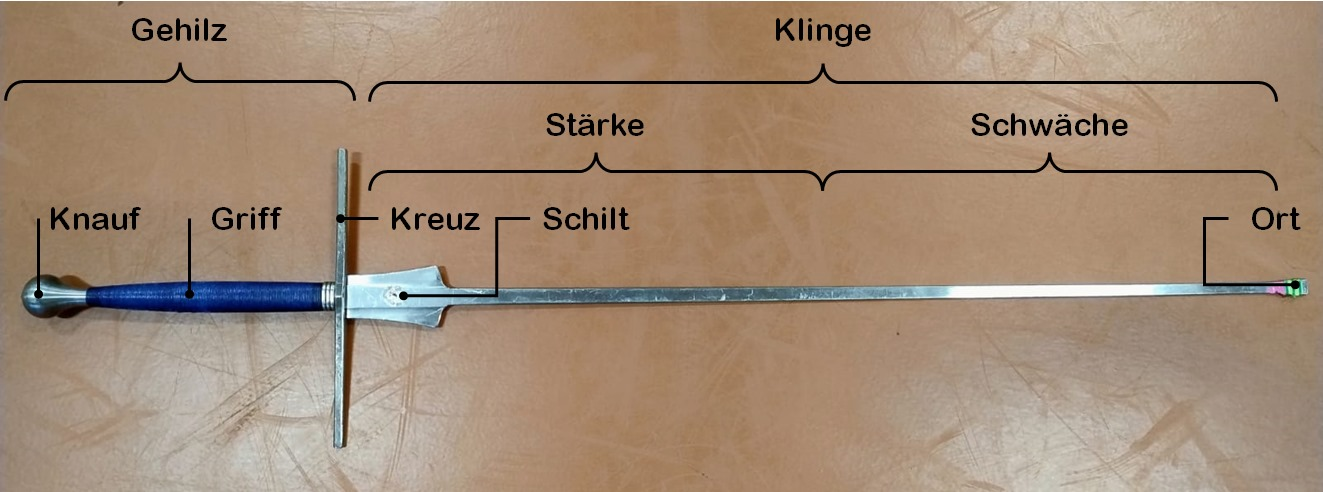
\includegraphics[scale=.35]{Nomenklatur.jpg}
    \caption{Die Nomenklatur des Schwertes}
    \label{fig:Schwert1}
\end{figure}

In \ref{fig:Schwert1} ist die Nomenklatur für das Schwert abgebildet. Die Klinge des Schwertes wird sowohl in Stärke und Schwäche, als auch in lange und kurze Schneide unterteilt. Beide Unterteilungen sind für die Bindungsarbeit wichtig und werden deshalb in den Kapiteln \ref{Bindung0} und \ref{Bindung1} ausführlich behandelt.

\FloatBarrier

\begin{figure}[ht!]
\minipage{0.38\textwidth}
  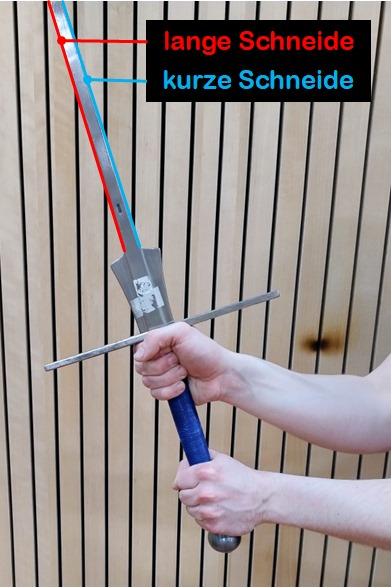
\includegraphics[width=\linewidth]{Hammergriff.jpg}
  \caption{Hammergriff}\label{fig:Hammergriff}
\endminipage\hfill
\minipage{0.38\textwidth}
  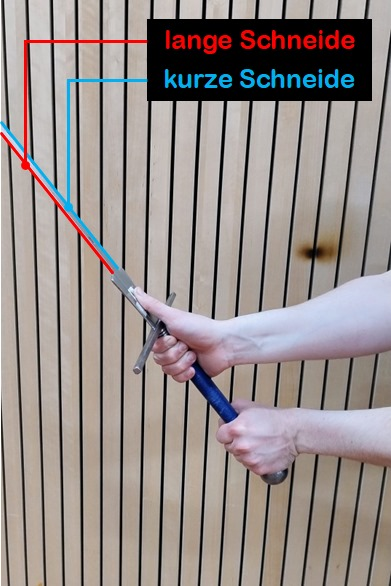
\includegraphics[width=\linewidth]{Daumengriff.jpg}
  \caption{Daumengriff}\label{fig:Daumengriff}
\endminipage\hfill
\end{figure}

Die Griffweise des Schwertes ist variabel. Die dominante Hand greift das Schwert am Griff, nahe des Kreuzes. Für diese Hand gibt es zwei grundlegende Griffweisen. Die erste kann als Hammergriff bezeichnet werden, bei dem bei dem die dominante Hand den Griff so greift, dass die Daumengabel in Linie mit dem Kreuz liegt. Die andere Griffweise heißt Daumengriff. Beim Daumengriff greift die dominante Hand den Griff so, dass der Daumen flach auf dem Kreuz oder Schilt liegt. Die zweite Hand umfasst in beiden Griffweisen den Griff im hinteren Drittel oder am Knauf und kann ihre Position verändern, sodass sich die Griffweise stets ergonomisch (niemals schmerzhaft!) anfühlt.
\\
\\
Die Unterteilung in Stärke und Schwäche richtet sich nach der Hebelwirkung, welche man mit der Klinge ausüben kann. Je länger der angewandte Lastarm wird, desto weniger Kraft kann man übertragen. Deshalb wird die Hälfte des Schwertes, welche weiter vom Hebelpunkt (dem Kreuz) entfernt ist, als Schwäche bezeichnet. Die näher am Kreuz gelegene Hälfte wird analog als Stärke bezeichnet. Das resultierende Kräfteverhältnis ist entscheidend für viele Fechtstücke.
\\
\\
Die Unterteilung in kurze und lange (manchmal ''wahre'' und ''falsche'') Schneide ist ebenfalls in der Bindungsarbeit wichtig und entspringt möglicherweise der Bezeichnung von Klingen (Säbel, Falchion), die tatsächlich zwei unterschiedlich lange Schneiden besitzen. Entsprechend der Griffweise dieser Waffen wird die Klinge, welche im Hammergriff in Richtung der Fingerknöchel zeigt stets als lange Schneide, und die Klinge welche in Richtung der Daumengabel zeigt als kurze Schneide bezeichnet. Im Daumengriff liegt die lange Schneide an den vordersten Fingerknöcheln, die kurze am Handrücken.

\subsubsection{Huten}

In der Tradition Liechtenauers werden vier Grundhaltungen unter dem Namen ''Hut'' (seltener Leger oder Lager) beschrieben. In diesen Huten schützt das Schwert jeweils einen klar definierten Bereich des Körpers, was dem Gegenüber nur begrenzte Möglichkeit gibt, durch eine direkte Aktion einen Treffer zu setzten. Gleichzeitig begünstigt die eigene Schwerthaltung manche Fechtstücke und erschwert andere. Das Wissen über die Möglichkeiten sowie Vor- und Nachteile der einzelnen Huten macht ein Gefecht berechenbarer und erleichtert den Eigenschutz. Es wird daher empfohlen, sich während des Gefechts dynamisch innerhalb dieser Huten zu bewegen und  diese als Anfangs- und Endpunkt der eignen Aktionen nutzen.
\\
\\
Liechtenauer und seine Anhänger unterscheiden also die vier grundlegenden Huten:
\enlargethispage{2\baselineskip}
\begin{itemize}
\item Vom Tag
\item Ochs
\item Pflug 
\item Alber (seltener Alba oder Olber) 
\end{itemize}

\hspace{1cm}
\\
Neben den Grundhuten werden später weitere Nebenhuten eingeführt (siehe Kap. \ref{Unten} und Kap. \ref{Wunder}), welche teils Übergangspositionen in Fechtstücken oder Ausgangsgangspunkt für spezielle Fechtstücke (meist in Tradition Liechtenauers aus der frühen Neuzeit) darstellen. 
Auch viele der Grundhuten können anhand der Schwertstellung weiter differenziert werden (Links / Rechts / Neutral). Wird in Texten keine Spezifizierung genannt, ist im Zweifel meist die neutrale oder rechte Variante gemeint.
\\
\\
Die Interpretation der Huten erfolgt größteils aus Bildquellen. Gemäß Maxime II sollte auch jeder für sich eine möglichst ergonomische und kraftsparende Auslegung finden. Nachfolgend ist jedoch eine kurze Bilderfolge der derzeitig prominentesten Interpretationen abgebildet.

\newpage

Als allgemeine Körperhaltung haben sich für alle Huten einige Gemeinsamkeiten etabliert.

\begin{itemize}
    \item Die Füße stehen etwas weiter als hüftweit, und zueinander etwa einen Gehschritt versetzt, um Gleichgewichtsverschiebungen schnell entgegentreten zu können.
    \item Beide Fußsohlen bleiben vollständig auf dem Boden.
 \item Wird das Schwert auf einer Seite gehalten, sollte stets der gegenüberliegende Fuß vorne stehen, um die Haubewegung besser unterstützen zu können.
 \item Der vordere Fuß zeigt zum Gegenüber (oder leicht nach außen), die hintere Fußspitze ist nach außen gedreht.
 \item Die Hüfte ist in den meisten Huten zum:zur Gegner:in ausgerichtet, sodass keine Hüftseite übermäßig zum Gegenüber zeigt. Außerdem ist sie leicht abgesenkt, sodass sich die Beine in eine minimale Hockbewegung begeben und dadurch leicht angespannt sind.
 \item Der Oberkörper ist gerade und leicht nach vorn gebeugt.
 \item Die Brustlinie richtet sich ebenfalls zum Gegnüber aus, sodass keine Schulter übermäßig zum:zur Gegner:in zeigt.
 \item Die Schultern sind leicht angespannt, sodass der Rücken keinen Buckel, aber auch kein Hohlkreuz bildet.
 \item Die Arme (speziell die Ellenbogen) bleiben nah am Körper, um kein Ziel zu bieten.
\end{itemize}

\newpage

\paragraph{Vom Tag}

\begin{figure}[ht!]
\minipage{0.32\textwidth}
  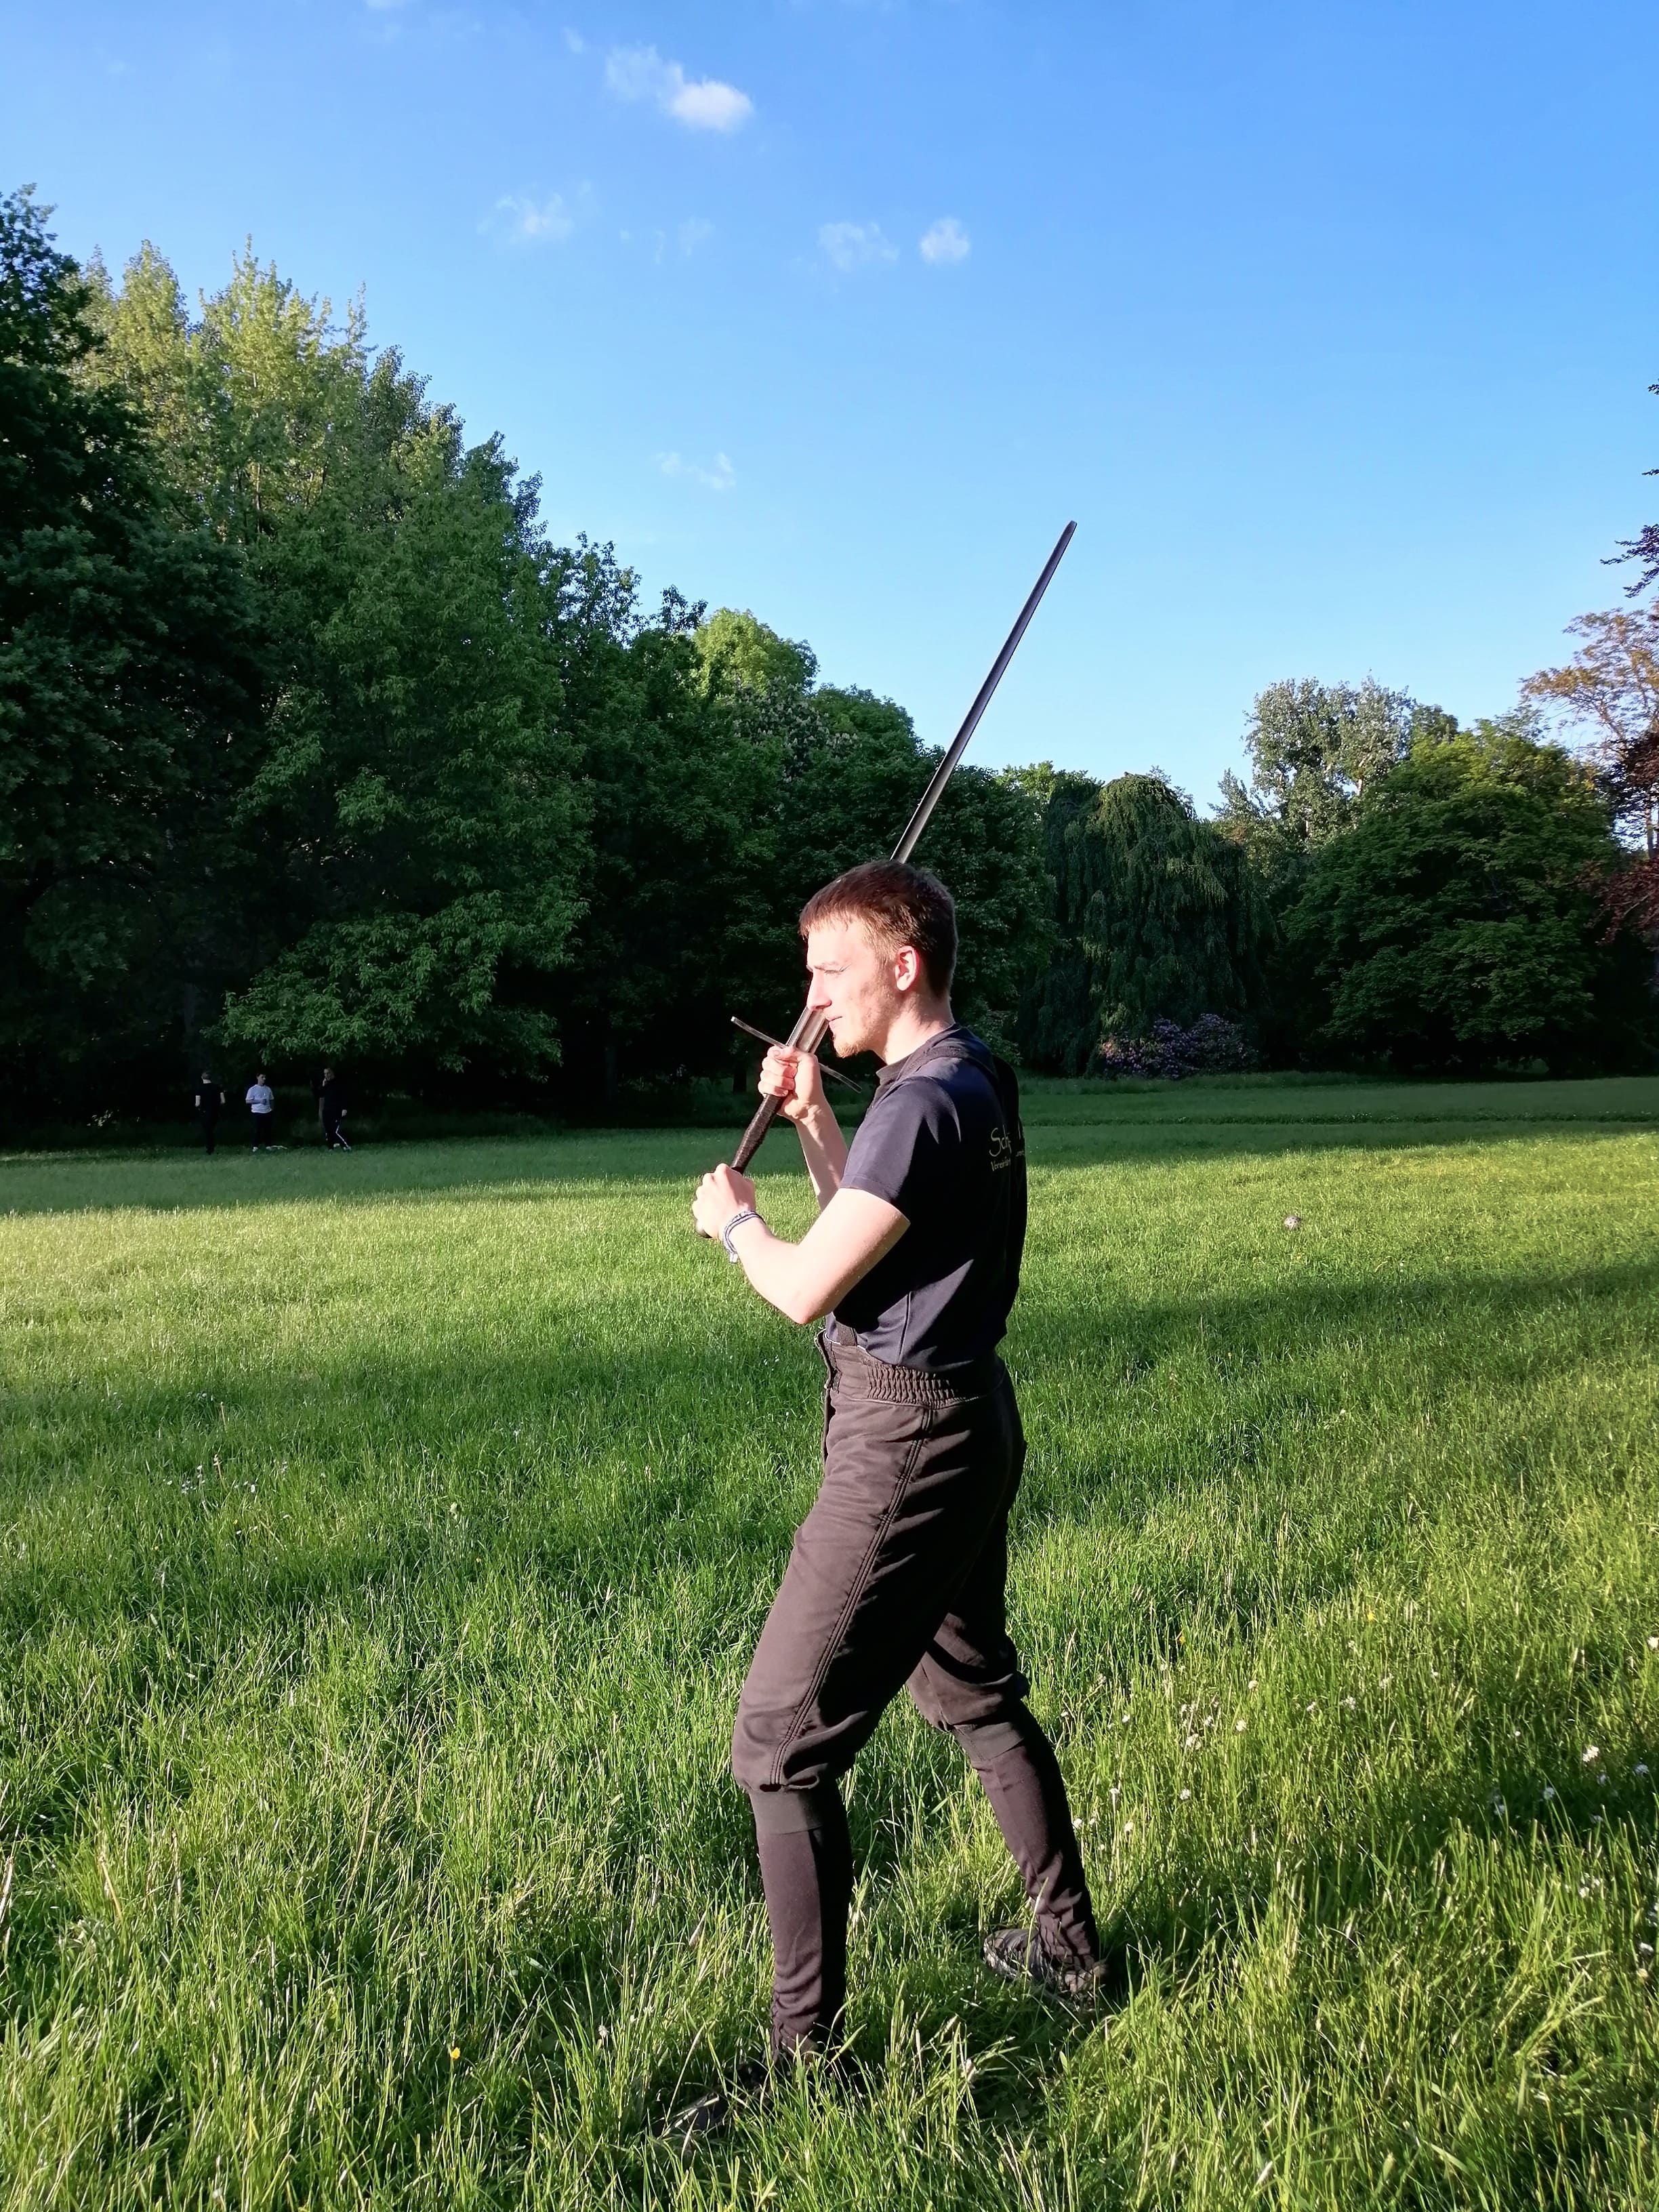
\includegraphics[width=\linewidth]{vonTag1.jpg}
  \caption{links}\label{fig:vt1}
\endminipage\hfill
\minipage{0.32\textwidth}
  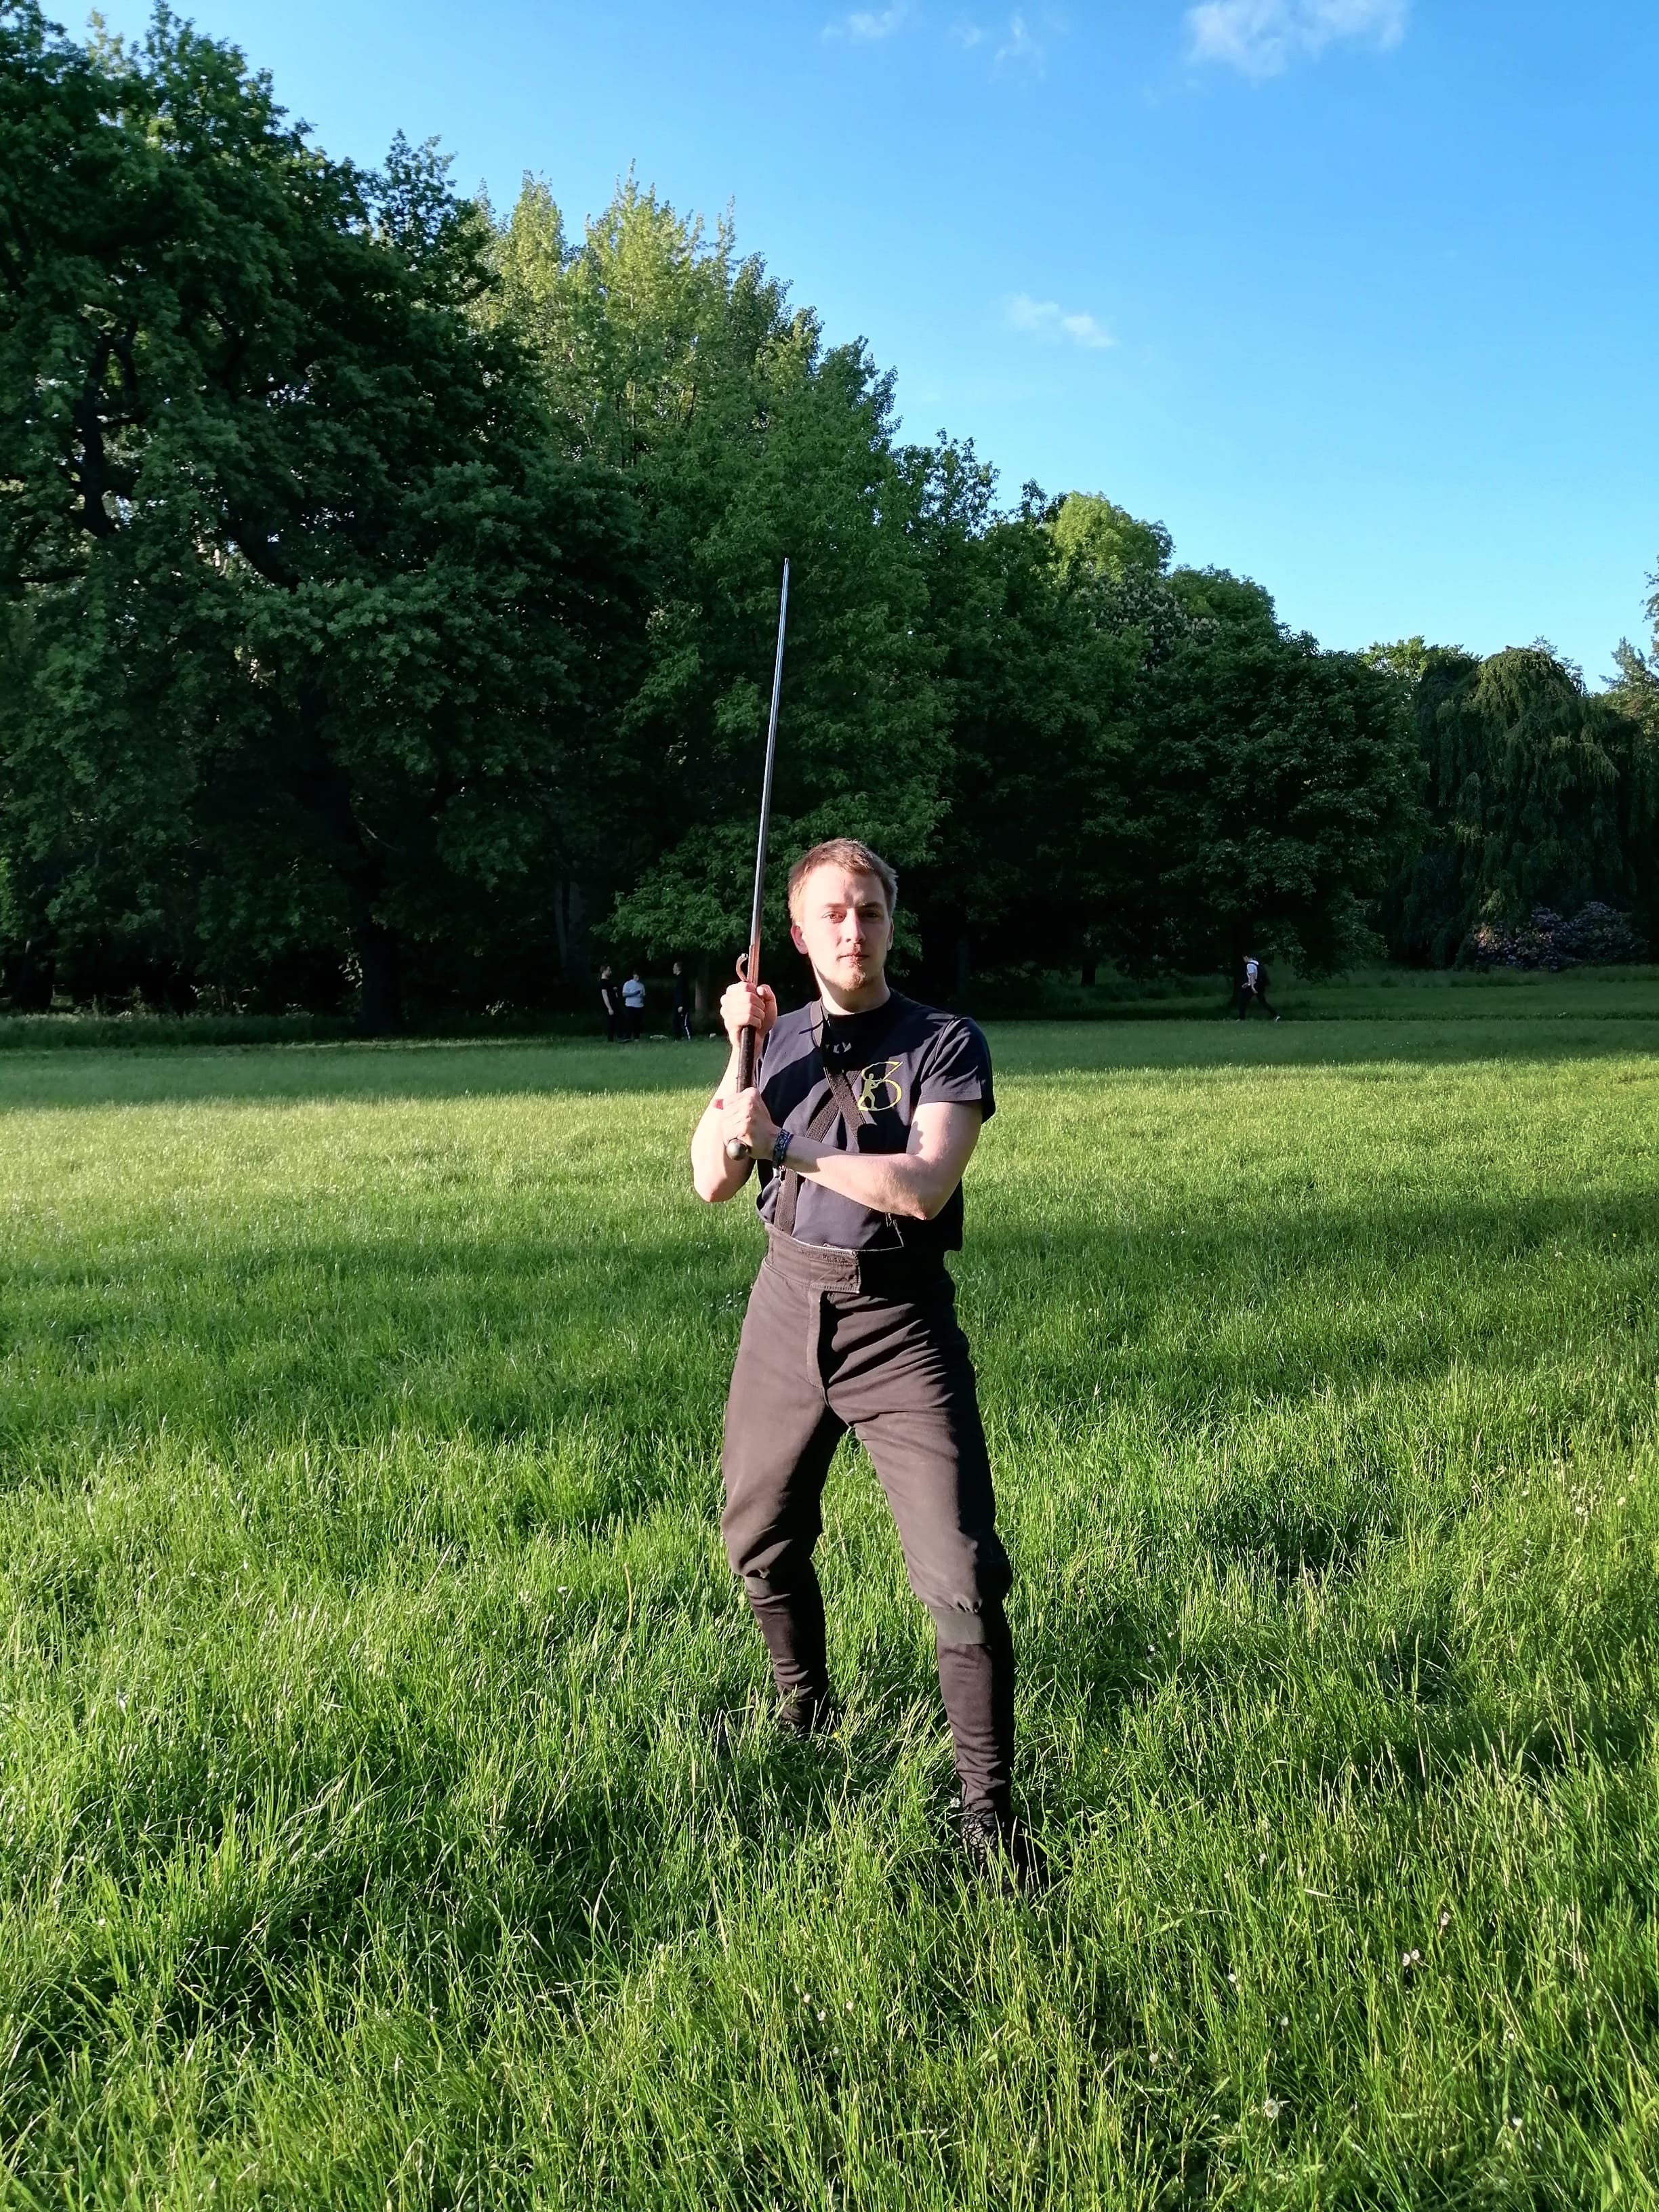
\includegraphics[width=\linewidth]{vonTag2.jpg}
  \caption{frontal}\label{fig:vt2}
\endminipage\hfill
\minipage{0.32\textwidth}%
  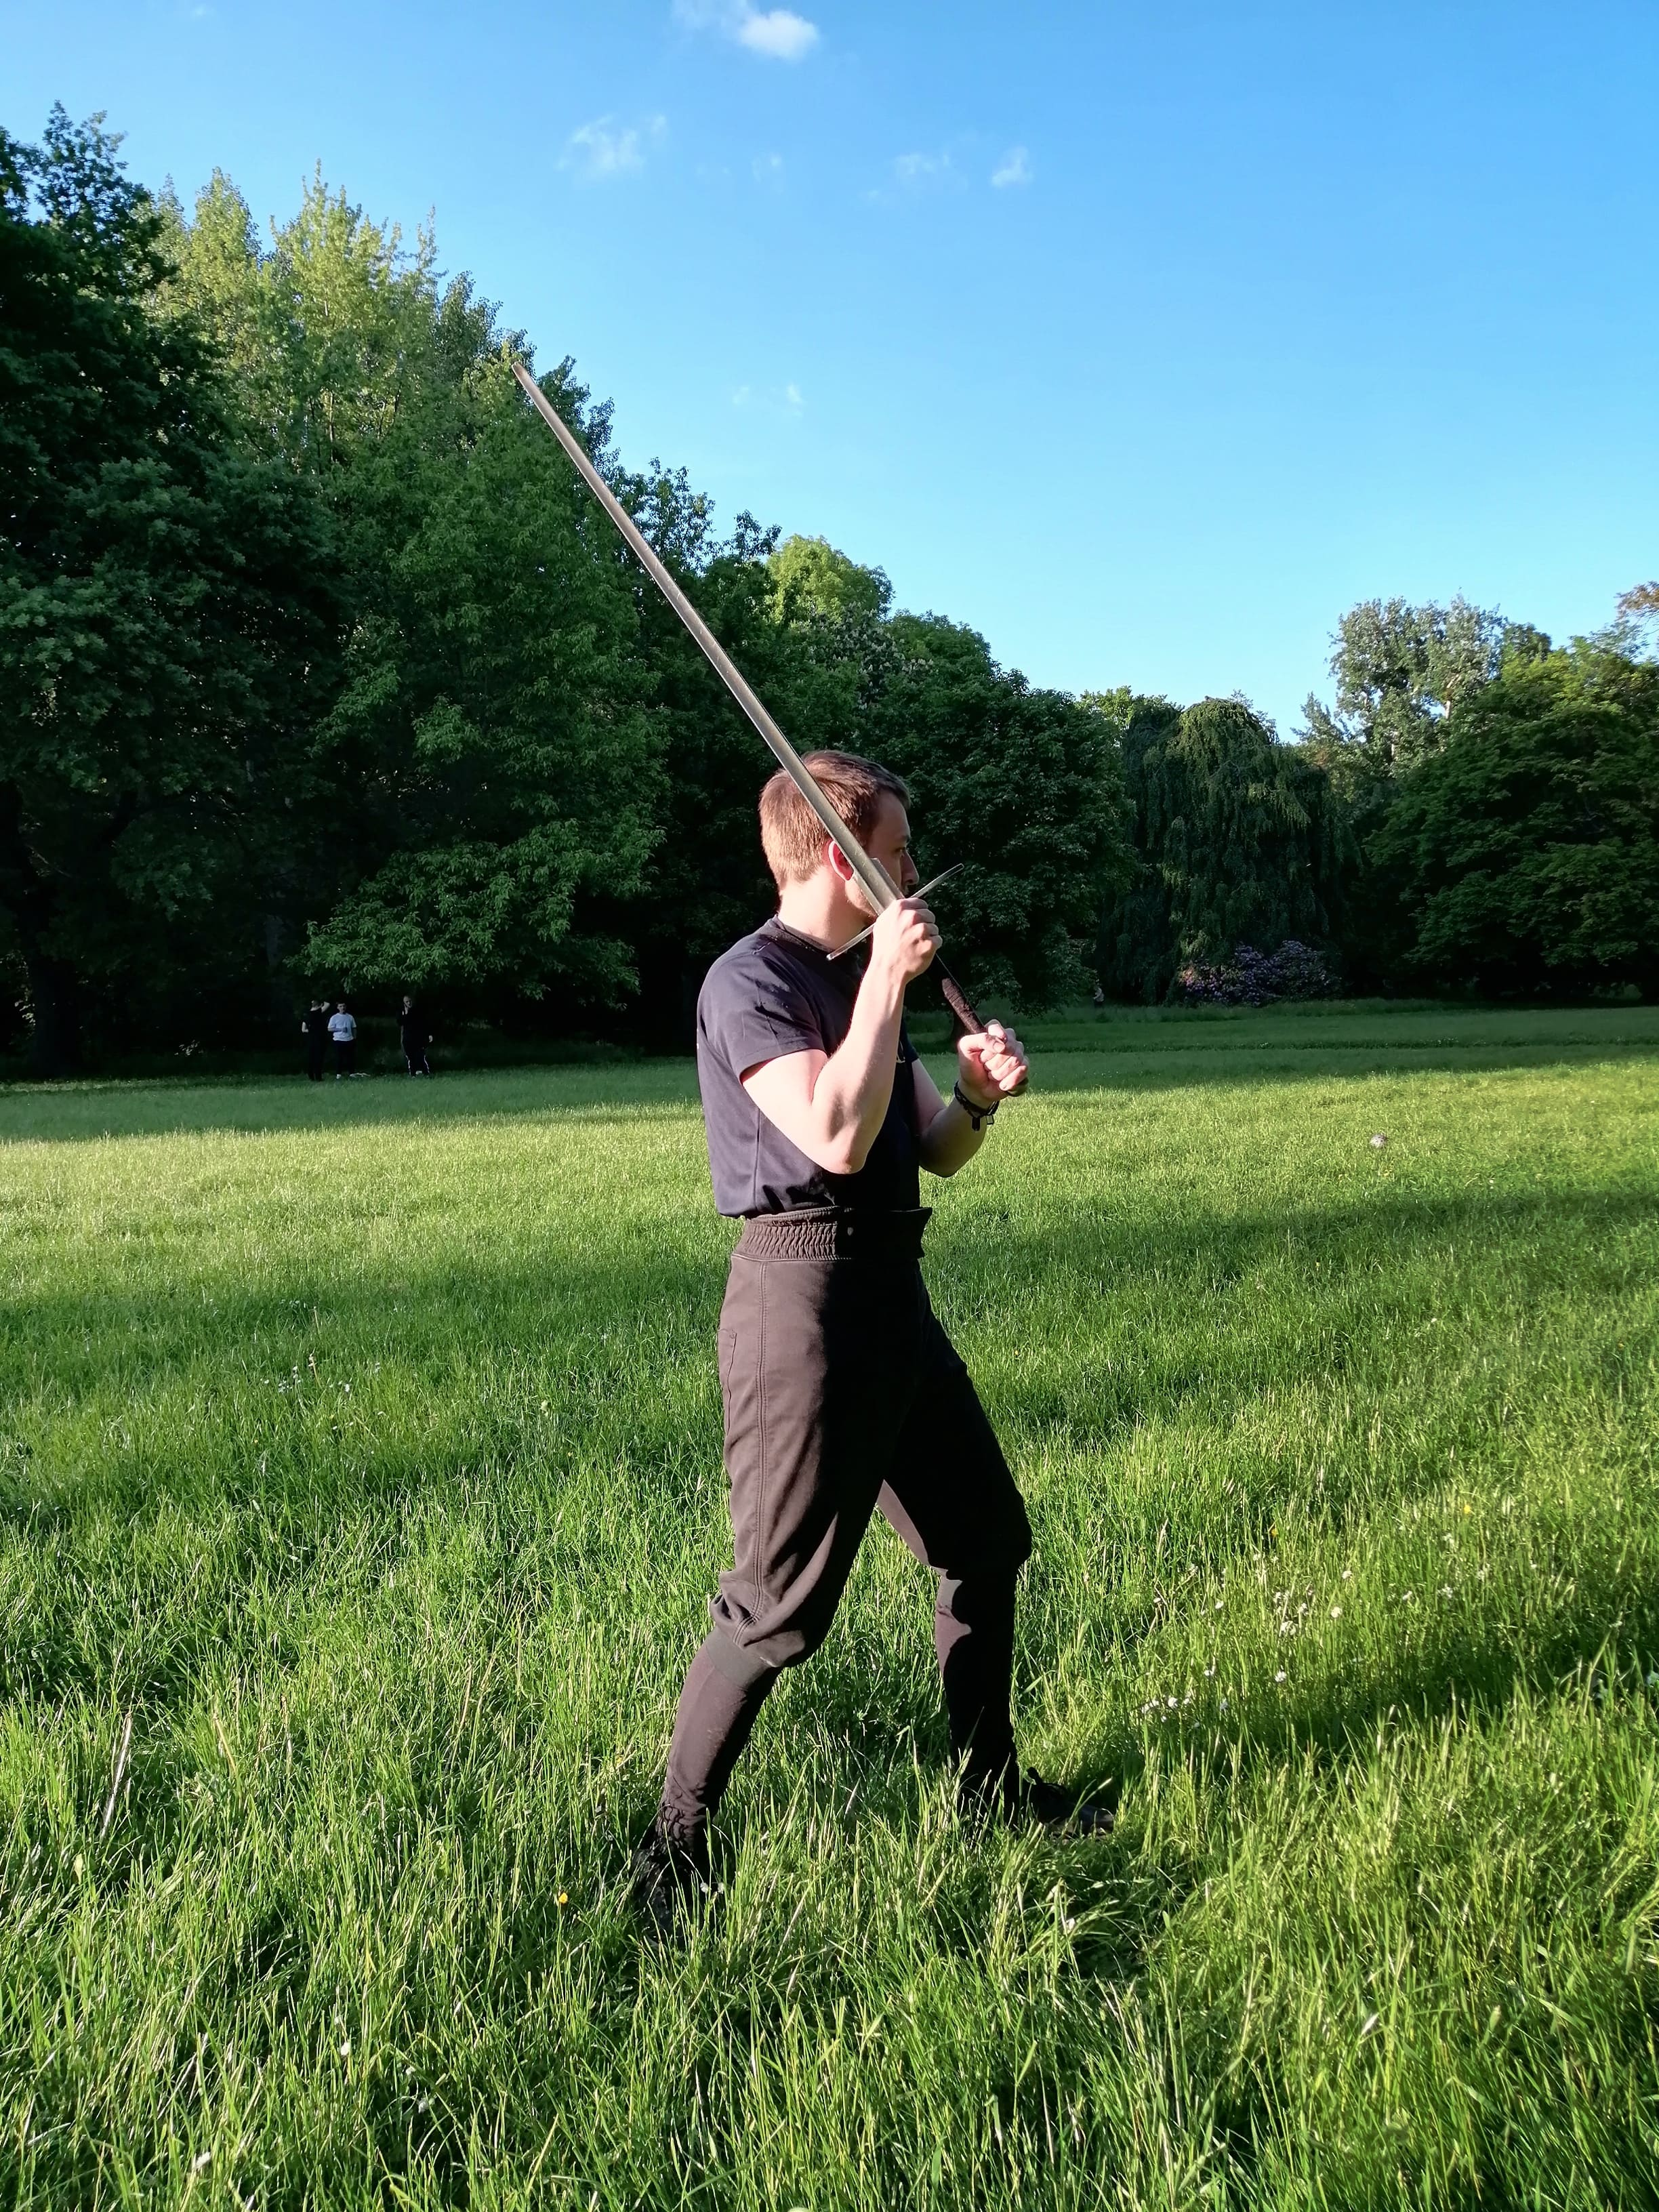
\includegraphics[width=\linewidth]{vonTag3.jpg}
  \caption{rechts}\label{fig:vt3}
\endminipage
\end{figure}

\FloatBarrier

Die Hut ''Vom Tag'' kann in drei Varianten unterteilt werden. Eine neutrale Position wird oft einfach ''Vom Tag'', seltener ''Vom Tag über Kopf'' genannt. Wird das Schwert auf einer Seite gehalten, fügt man dieser Seite den Namen hinzu ''Vom Tag, (Schulter) rechts / links''. Beide Seiten werden identisch ausgeführt, jedoch gespiegelt. Das Schwert wird vorzugsweise im Hammergriff gehalten.
\\
\hrule

\paragraph{Pflug}

\begin{figure}[ht!]
\minipage{0.32\textwidth}
  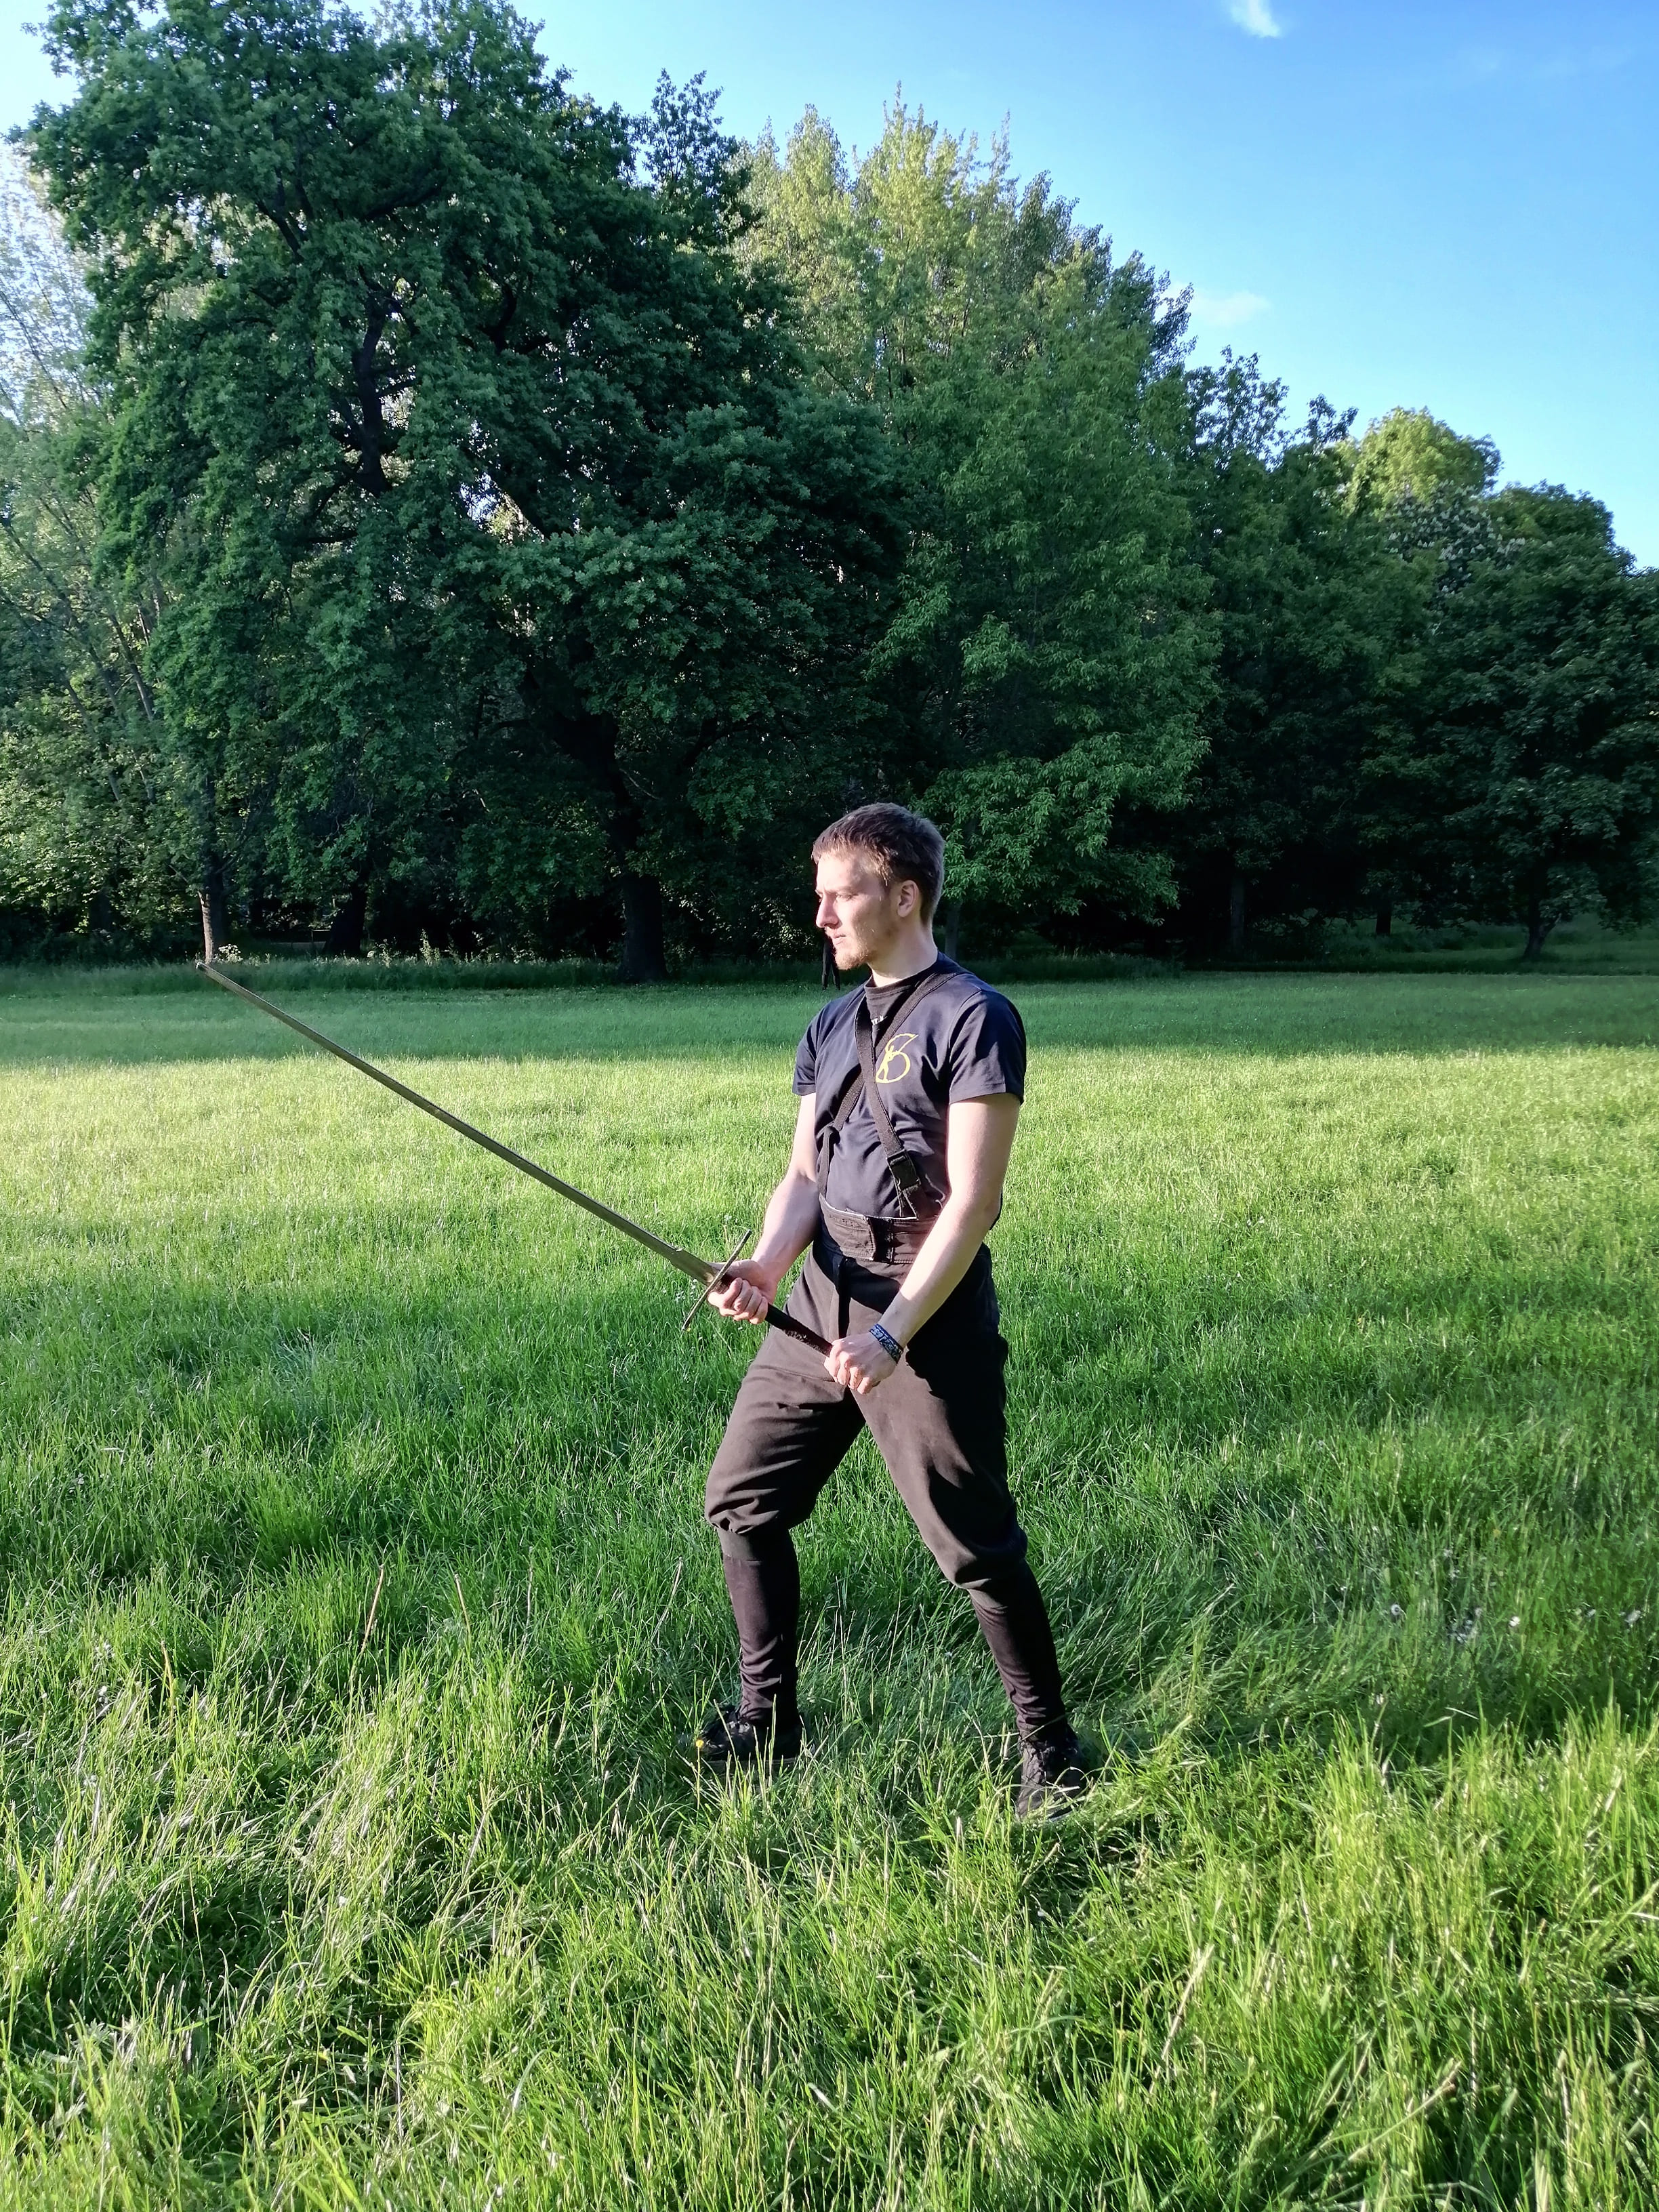
\includegraphics[width=\linewidth]{Pflug1.jpg}
  \caption{links}\label{fig:pflug1}
\endminipage\hfill
\minipage{0.32\textwidth}
  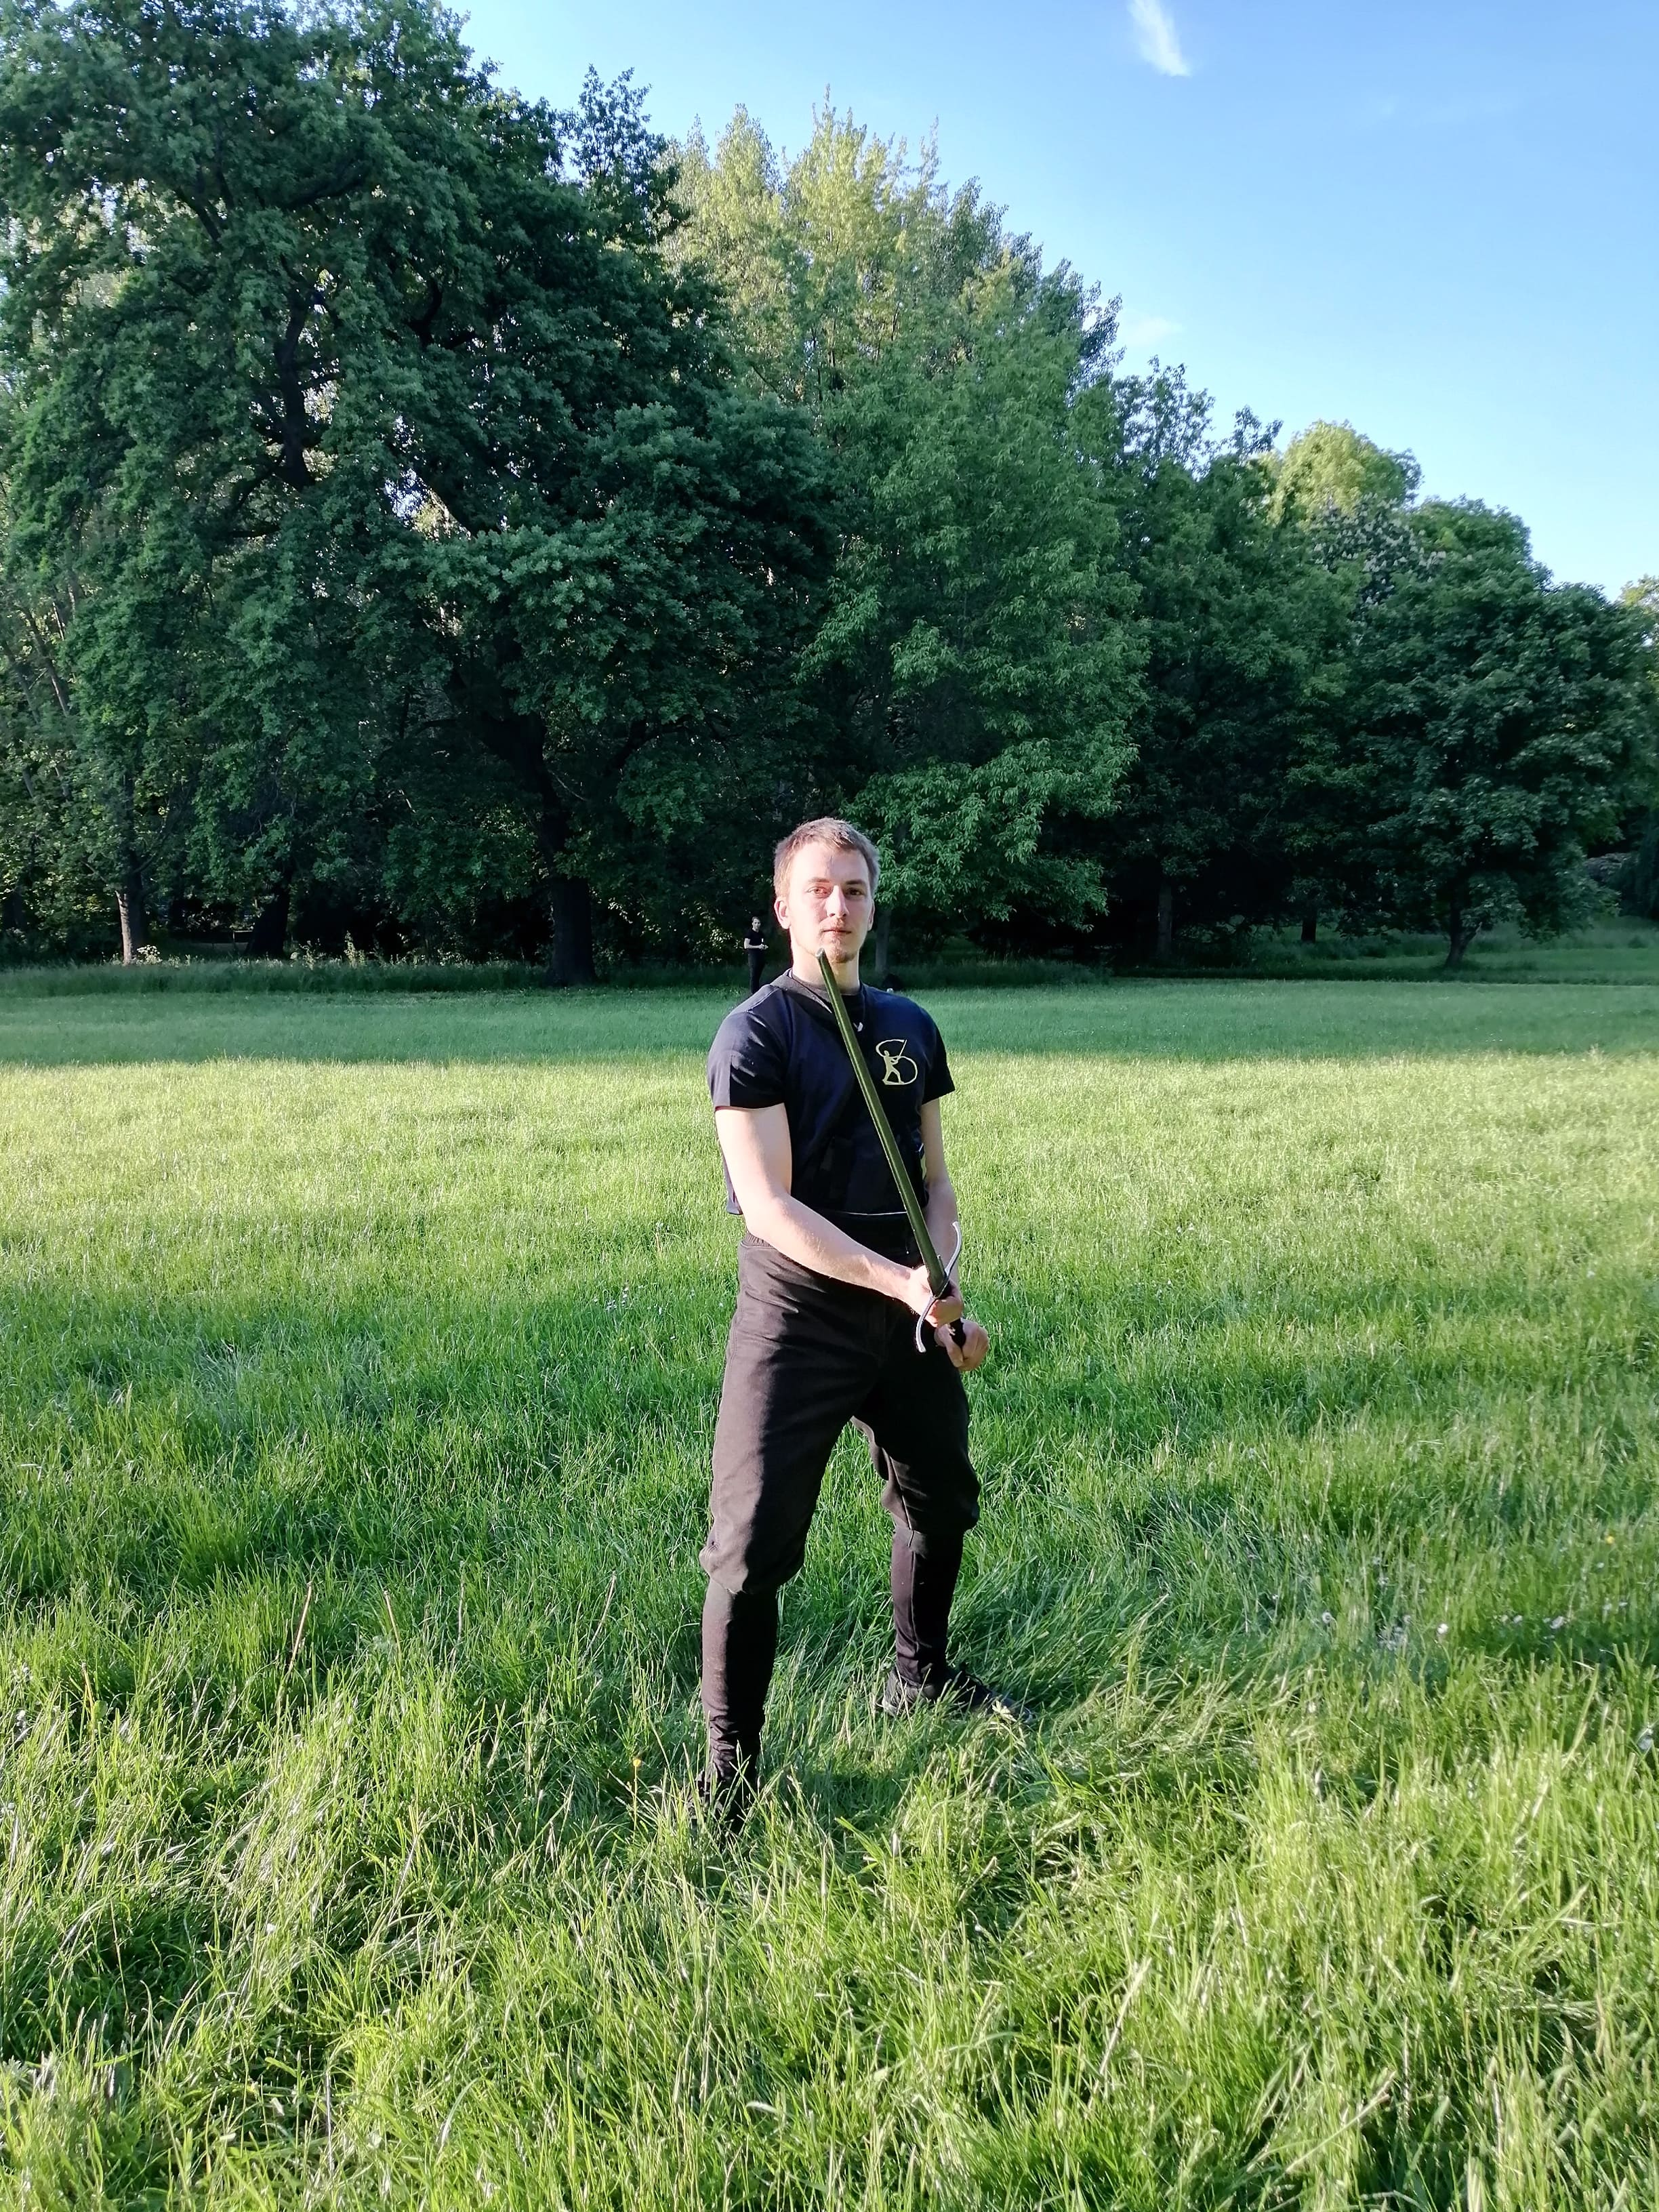
\includegraphics[width=\linewidth]{Pflug2.jpg}
  \caption{frontal}\label{fig:pflug2}
\endminipage\hfill
\minipage{0.32\textwidth}%
  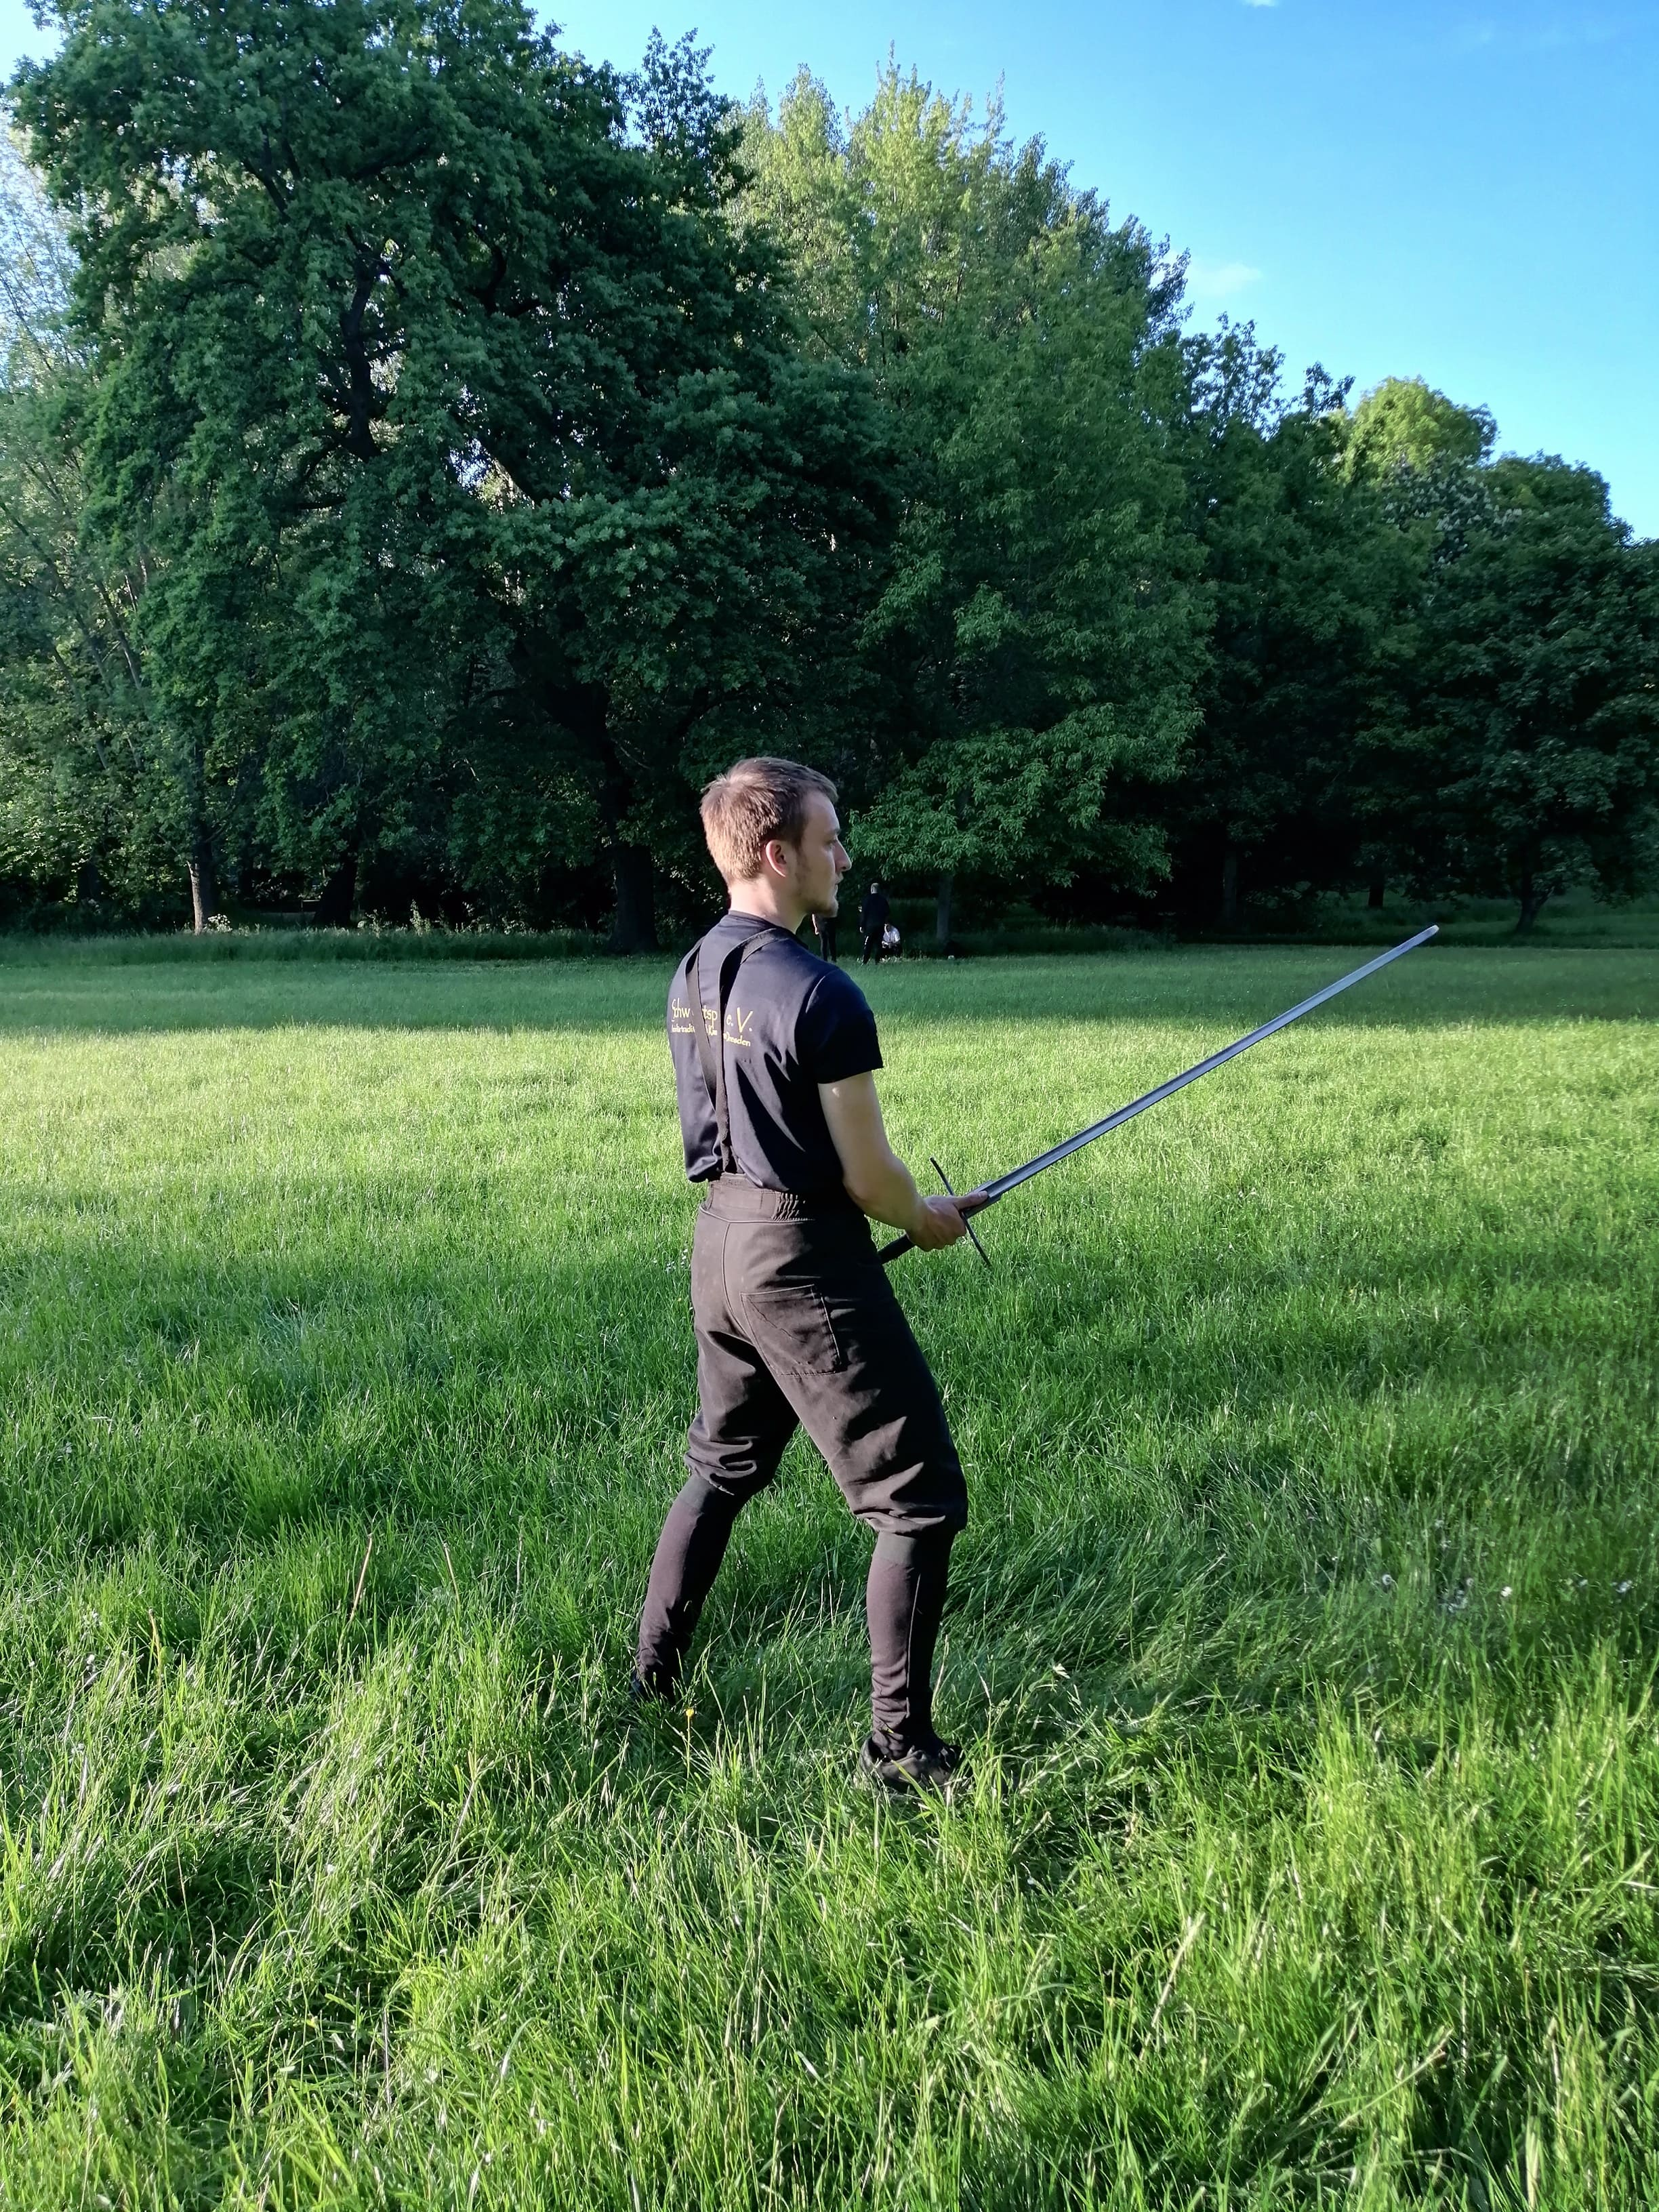
\includegraphics[width=\linewidth]{Pflug3.jpg}
  \caption{rechts}\label{fig:pflug3}
\endminipage
\end{figure}

\FloatBarrier

Die Hut ''Plfug'' wird ebenfalls in links und rechts unterschieden. Beide Seiten werden identisch ausgeführt, jedoch gespiegelt. Das Schwert wird oft im Daumengriff gehalten.

\clearpage

\paragraph{Ochs}

\begin{figure}[h!t]
\minipage{0.32\textwidth}
  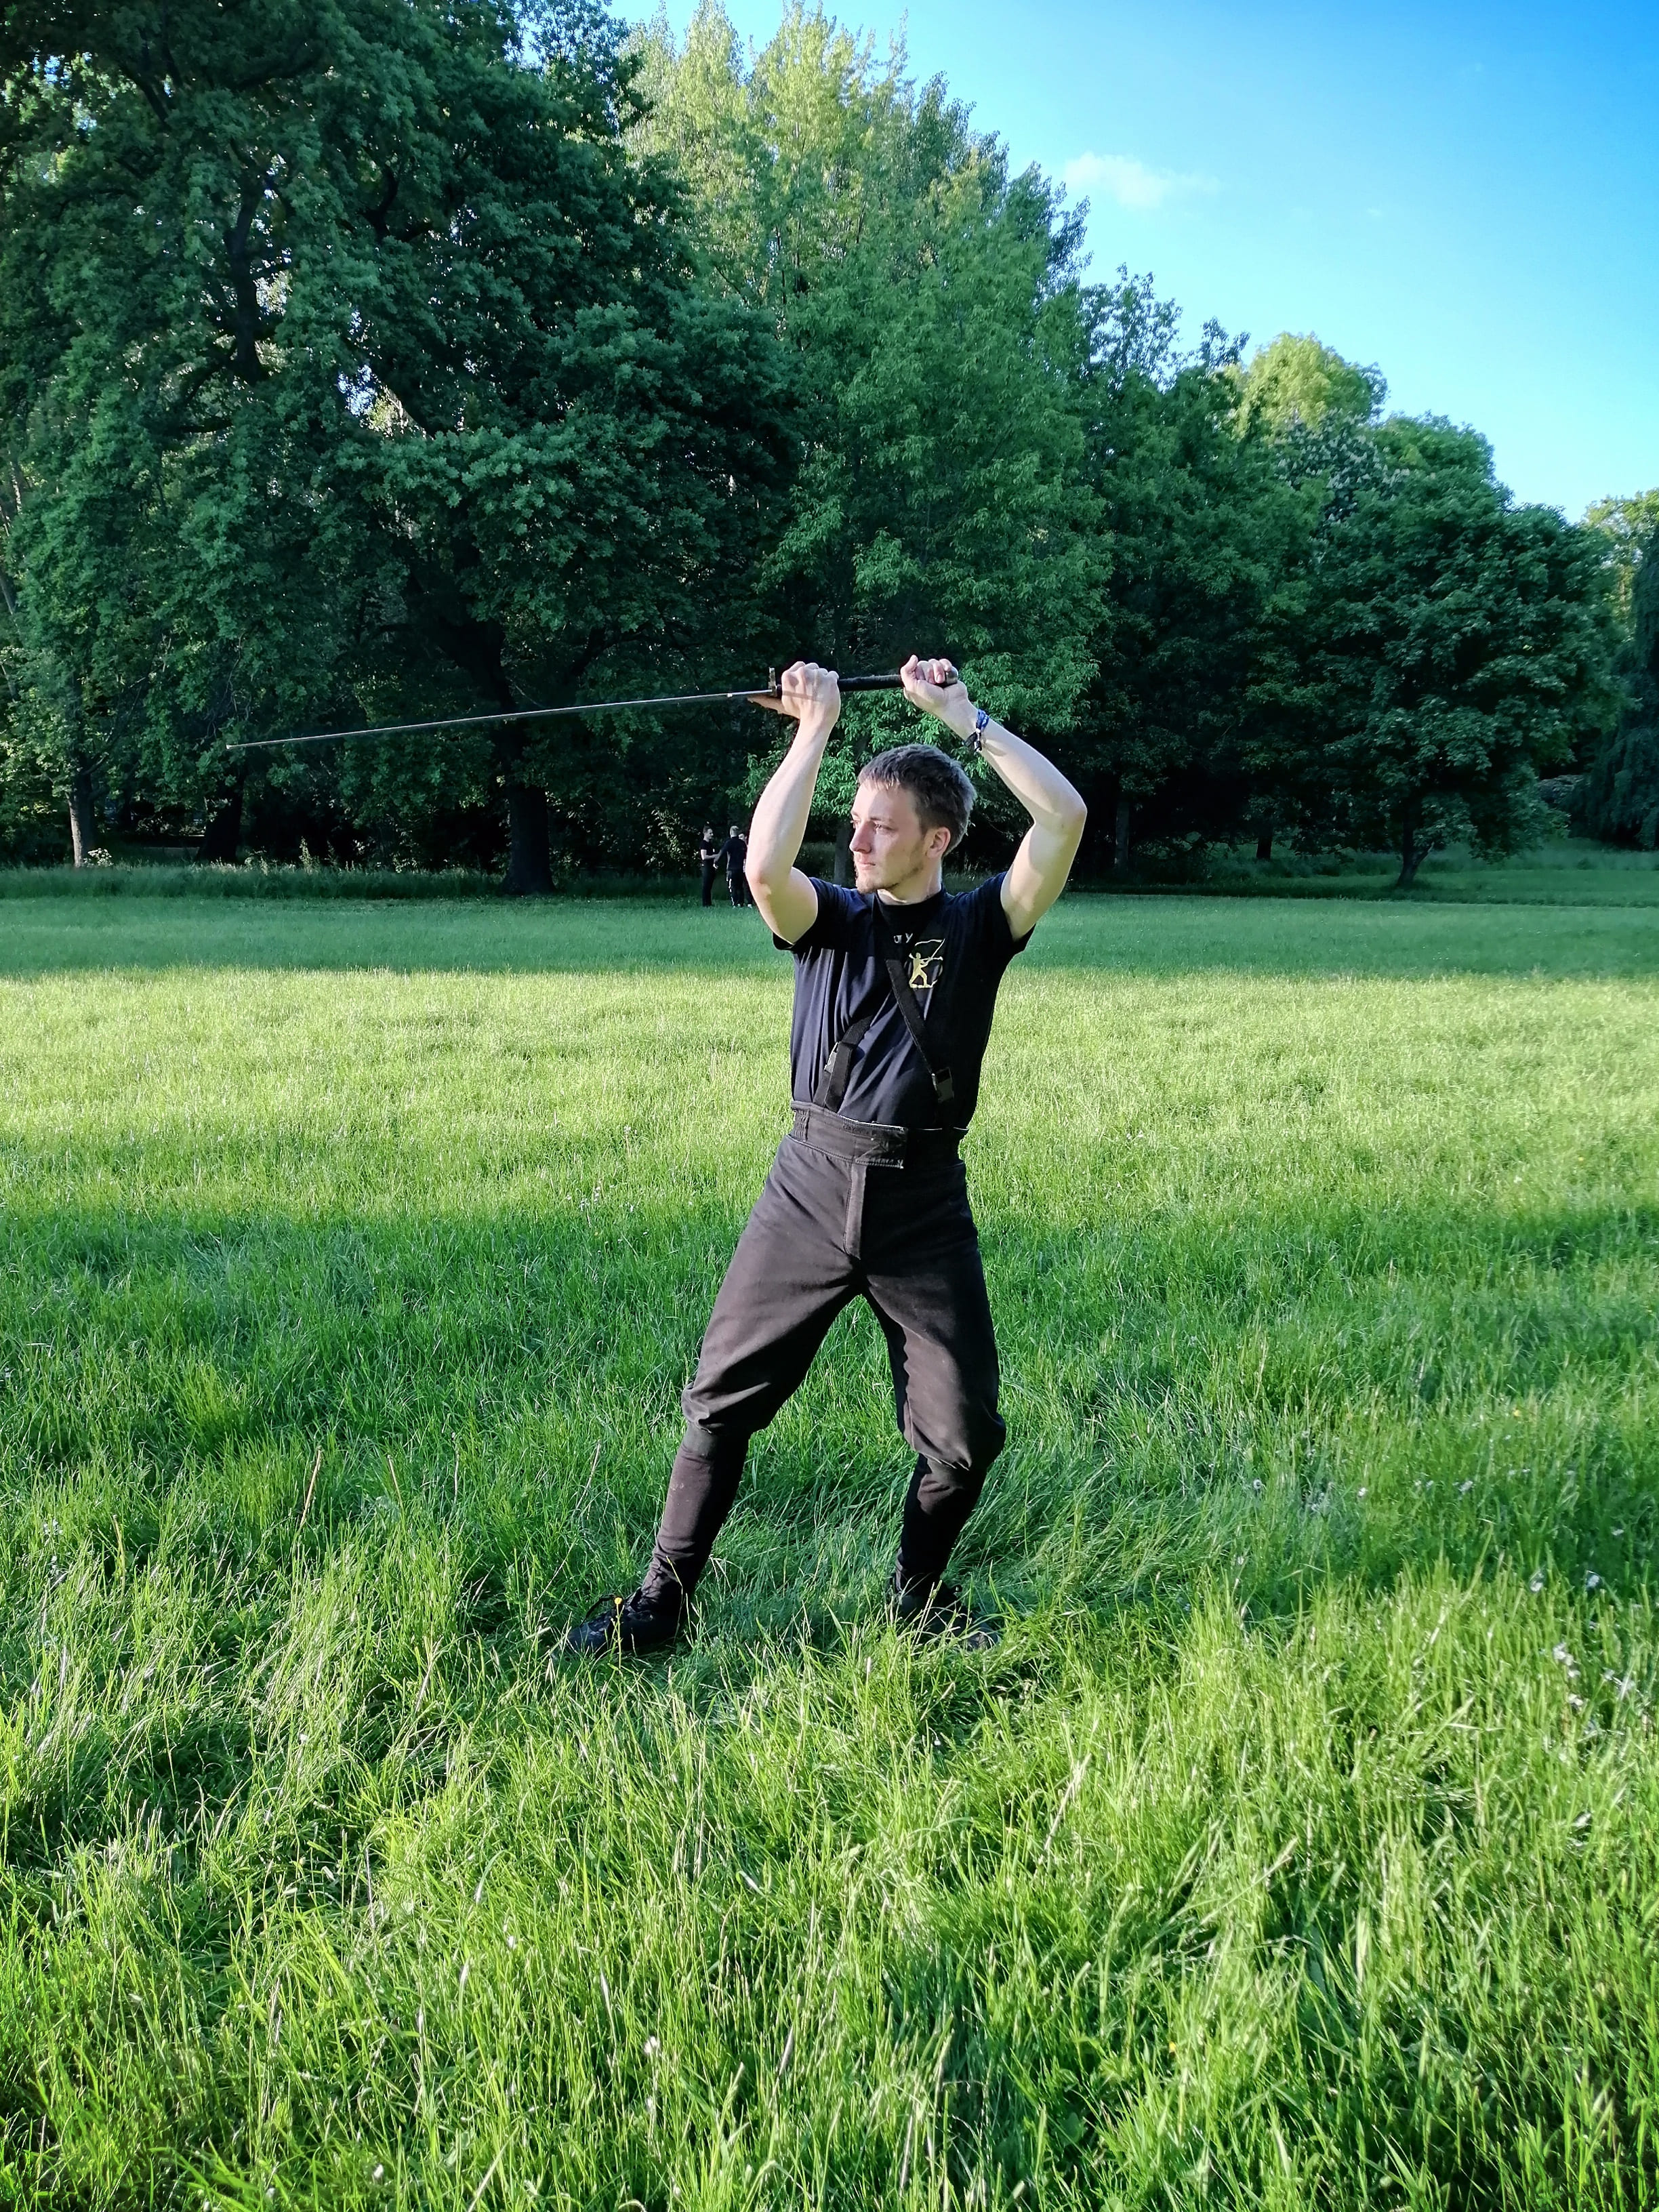
\includegraphics[width=\linewidth]{Ochs1.jpg}
  \caption{Ochs links}\label{fig:ochs1}
\endminipage\hfill
\minipage{0.32\textwidth}
  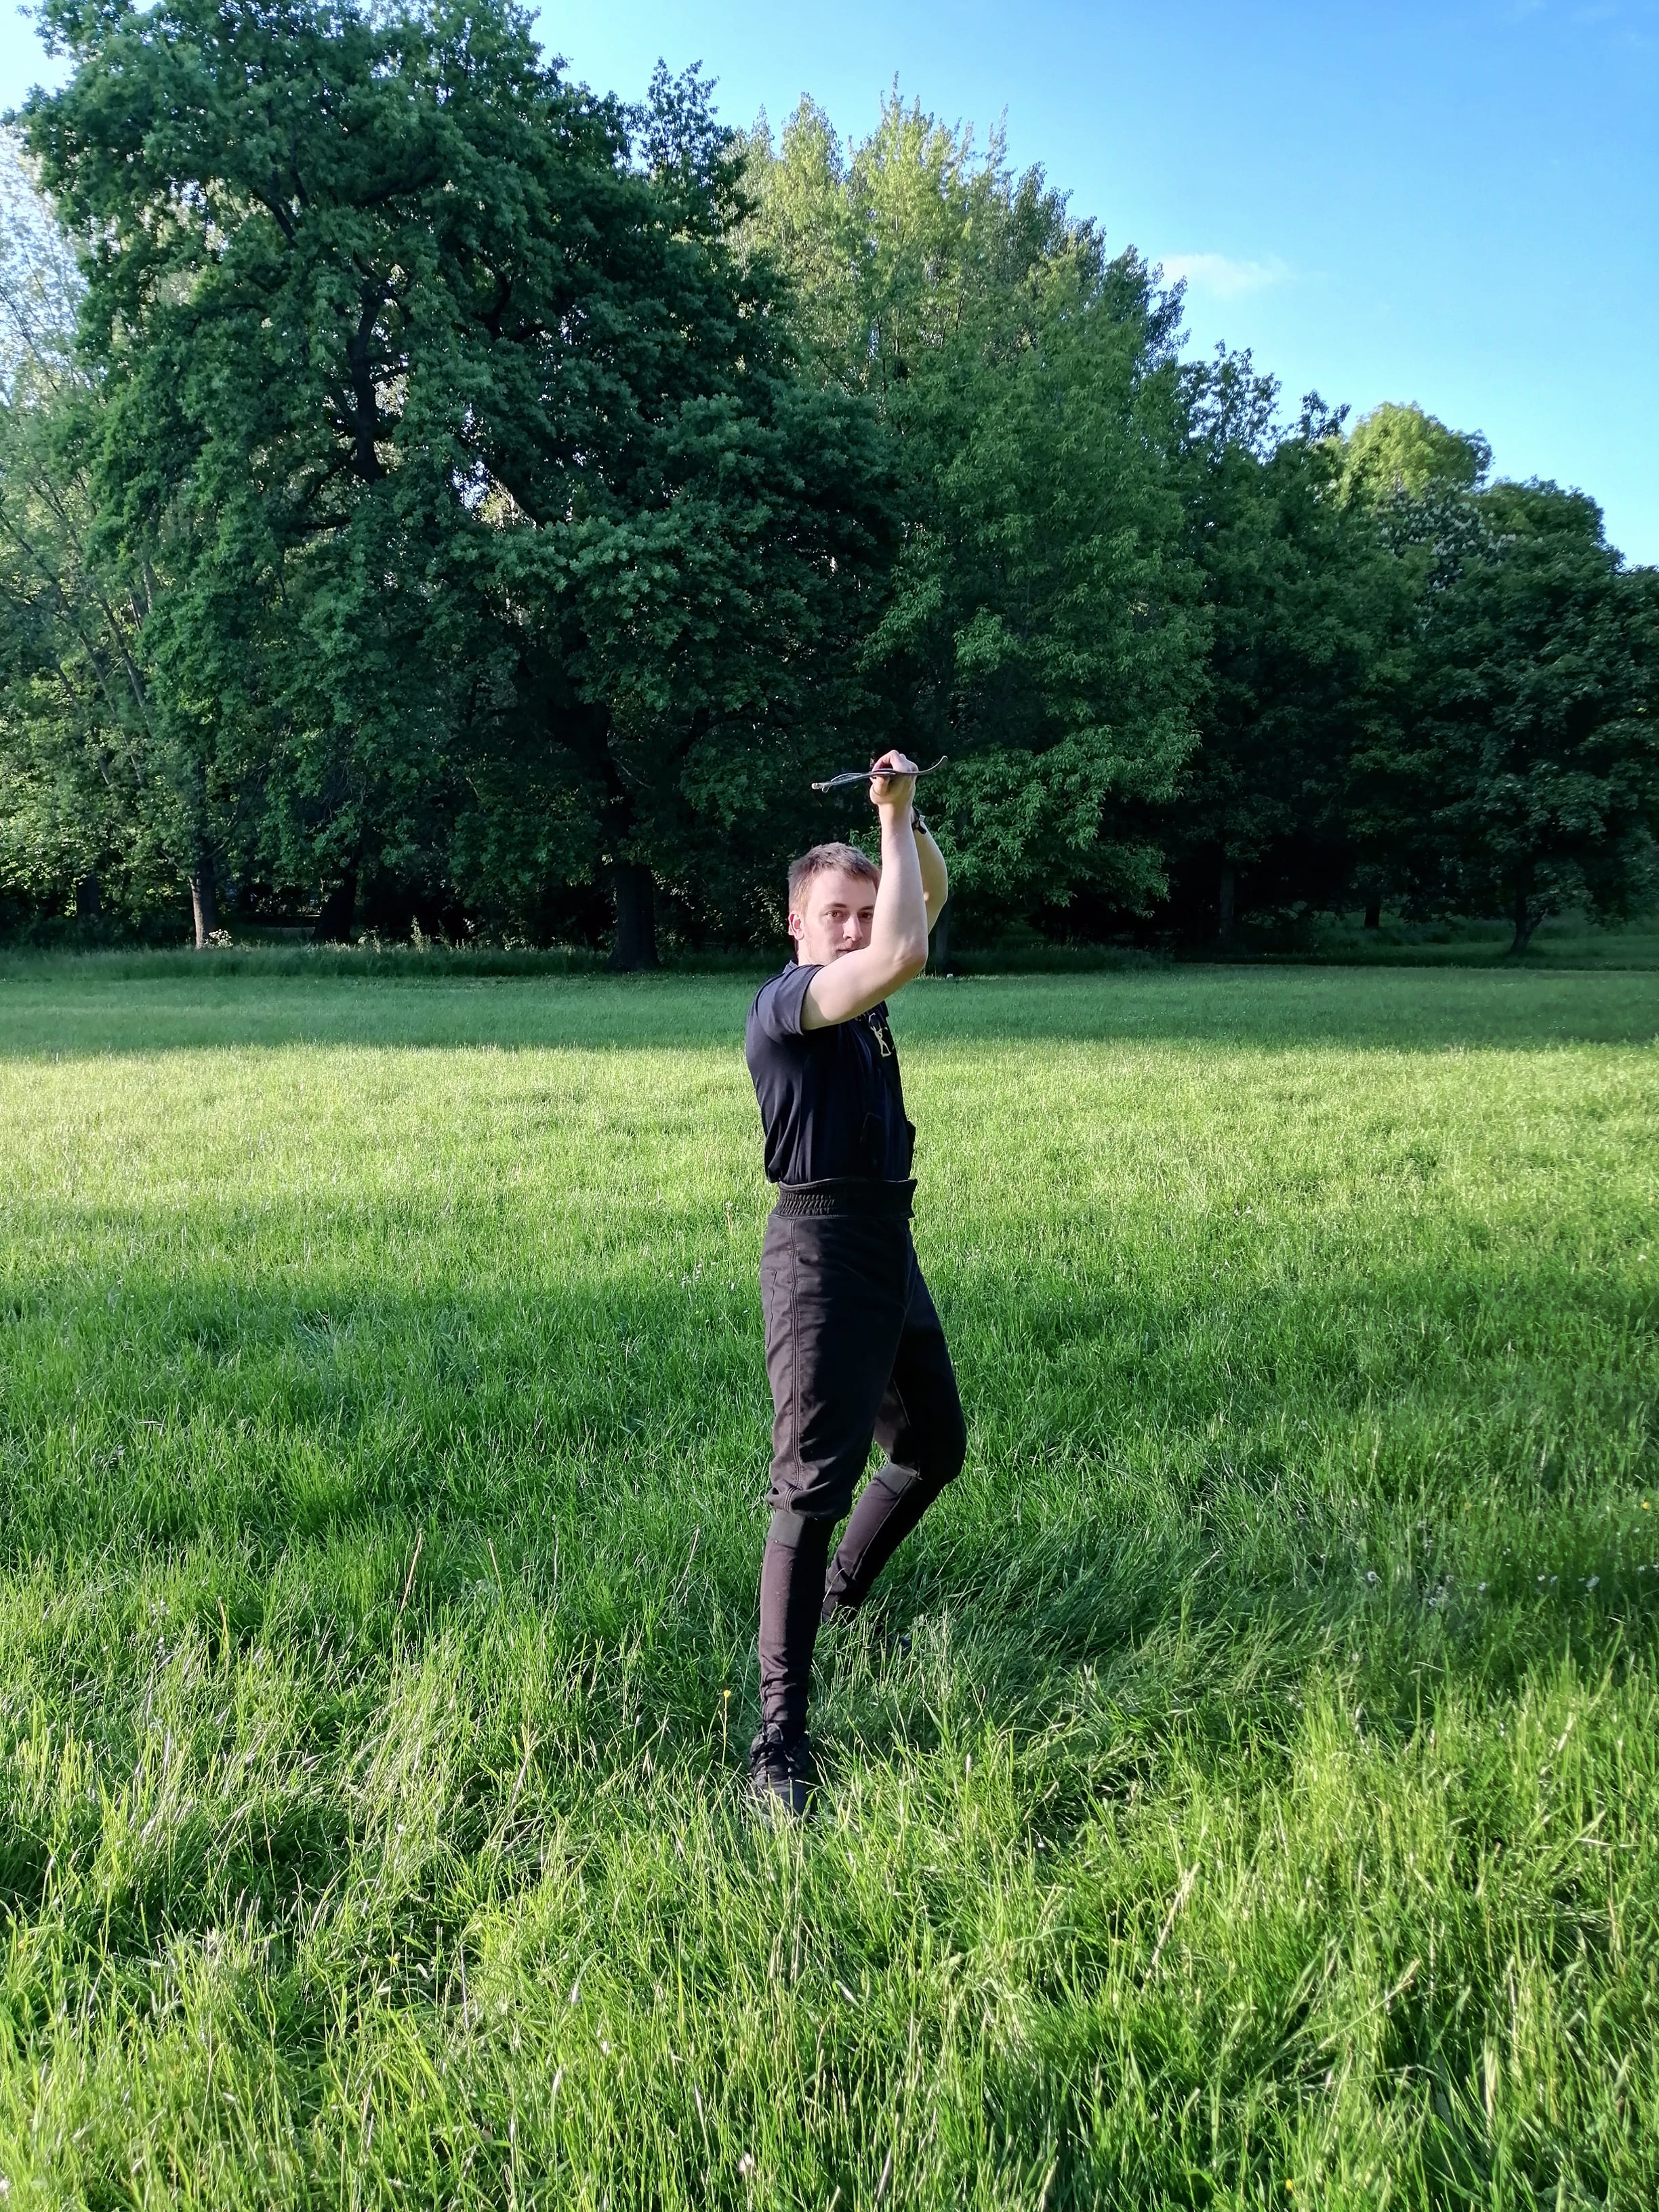
\includegraphics[width=\linewidth]{Ochs2.jpg}
  \caption{Ochs links}\label{fig:ochs2}
\endminipage\hfill
\minipage{0.32\textwidth}%
  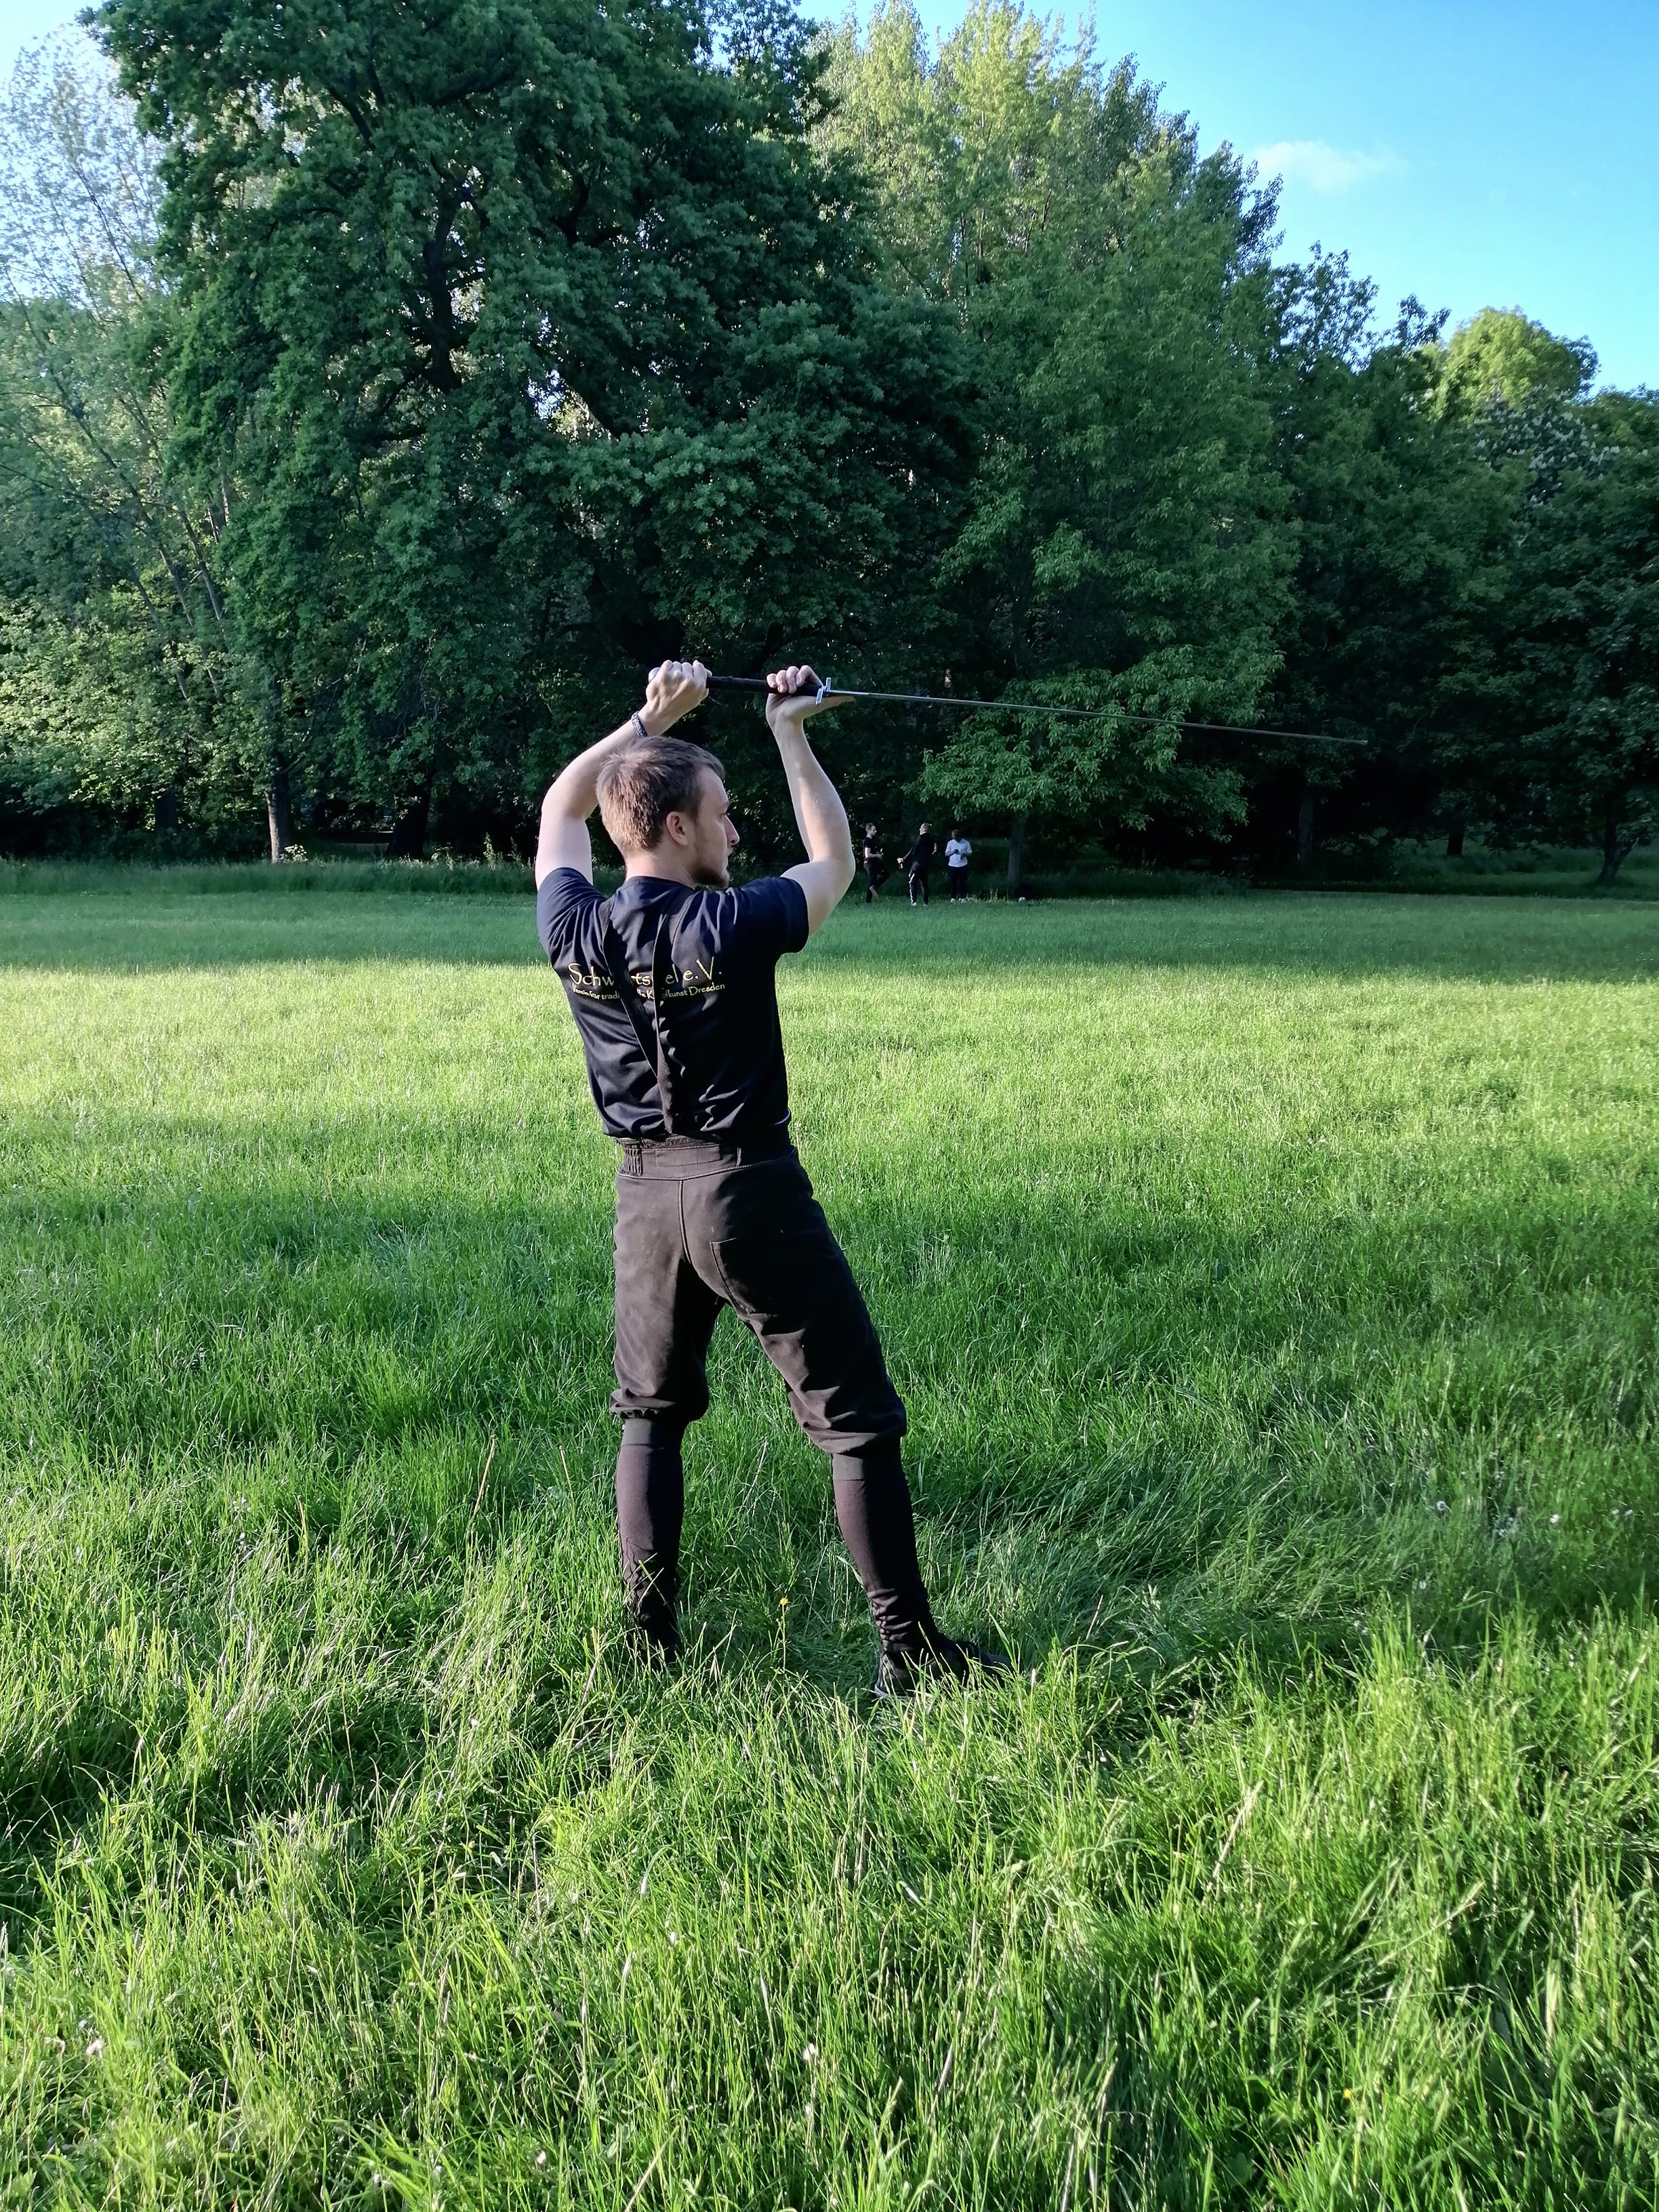
\includegraphics[width=\linewidth]{Ochs3.jpg}
  \caption{Ochs links}\label{fig:ochs3}
\endminipage
\end{figure}
\begin{figure}[ht!]
\minipage{0.32\textwidth}
  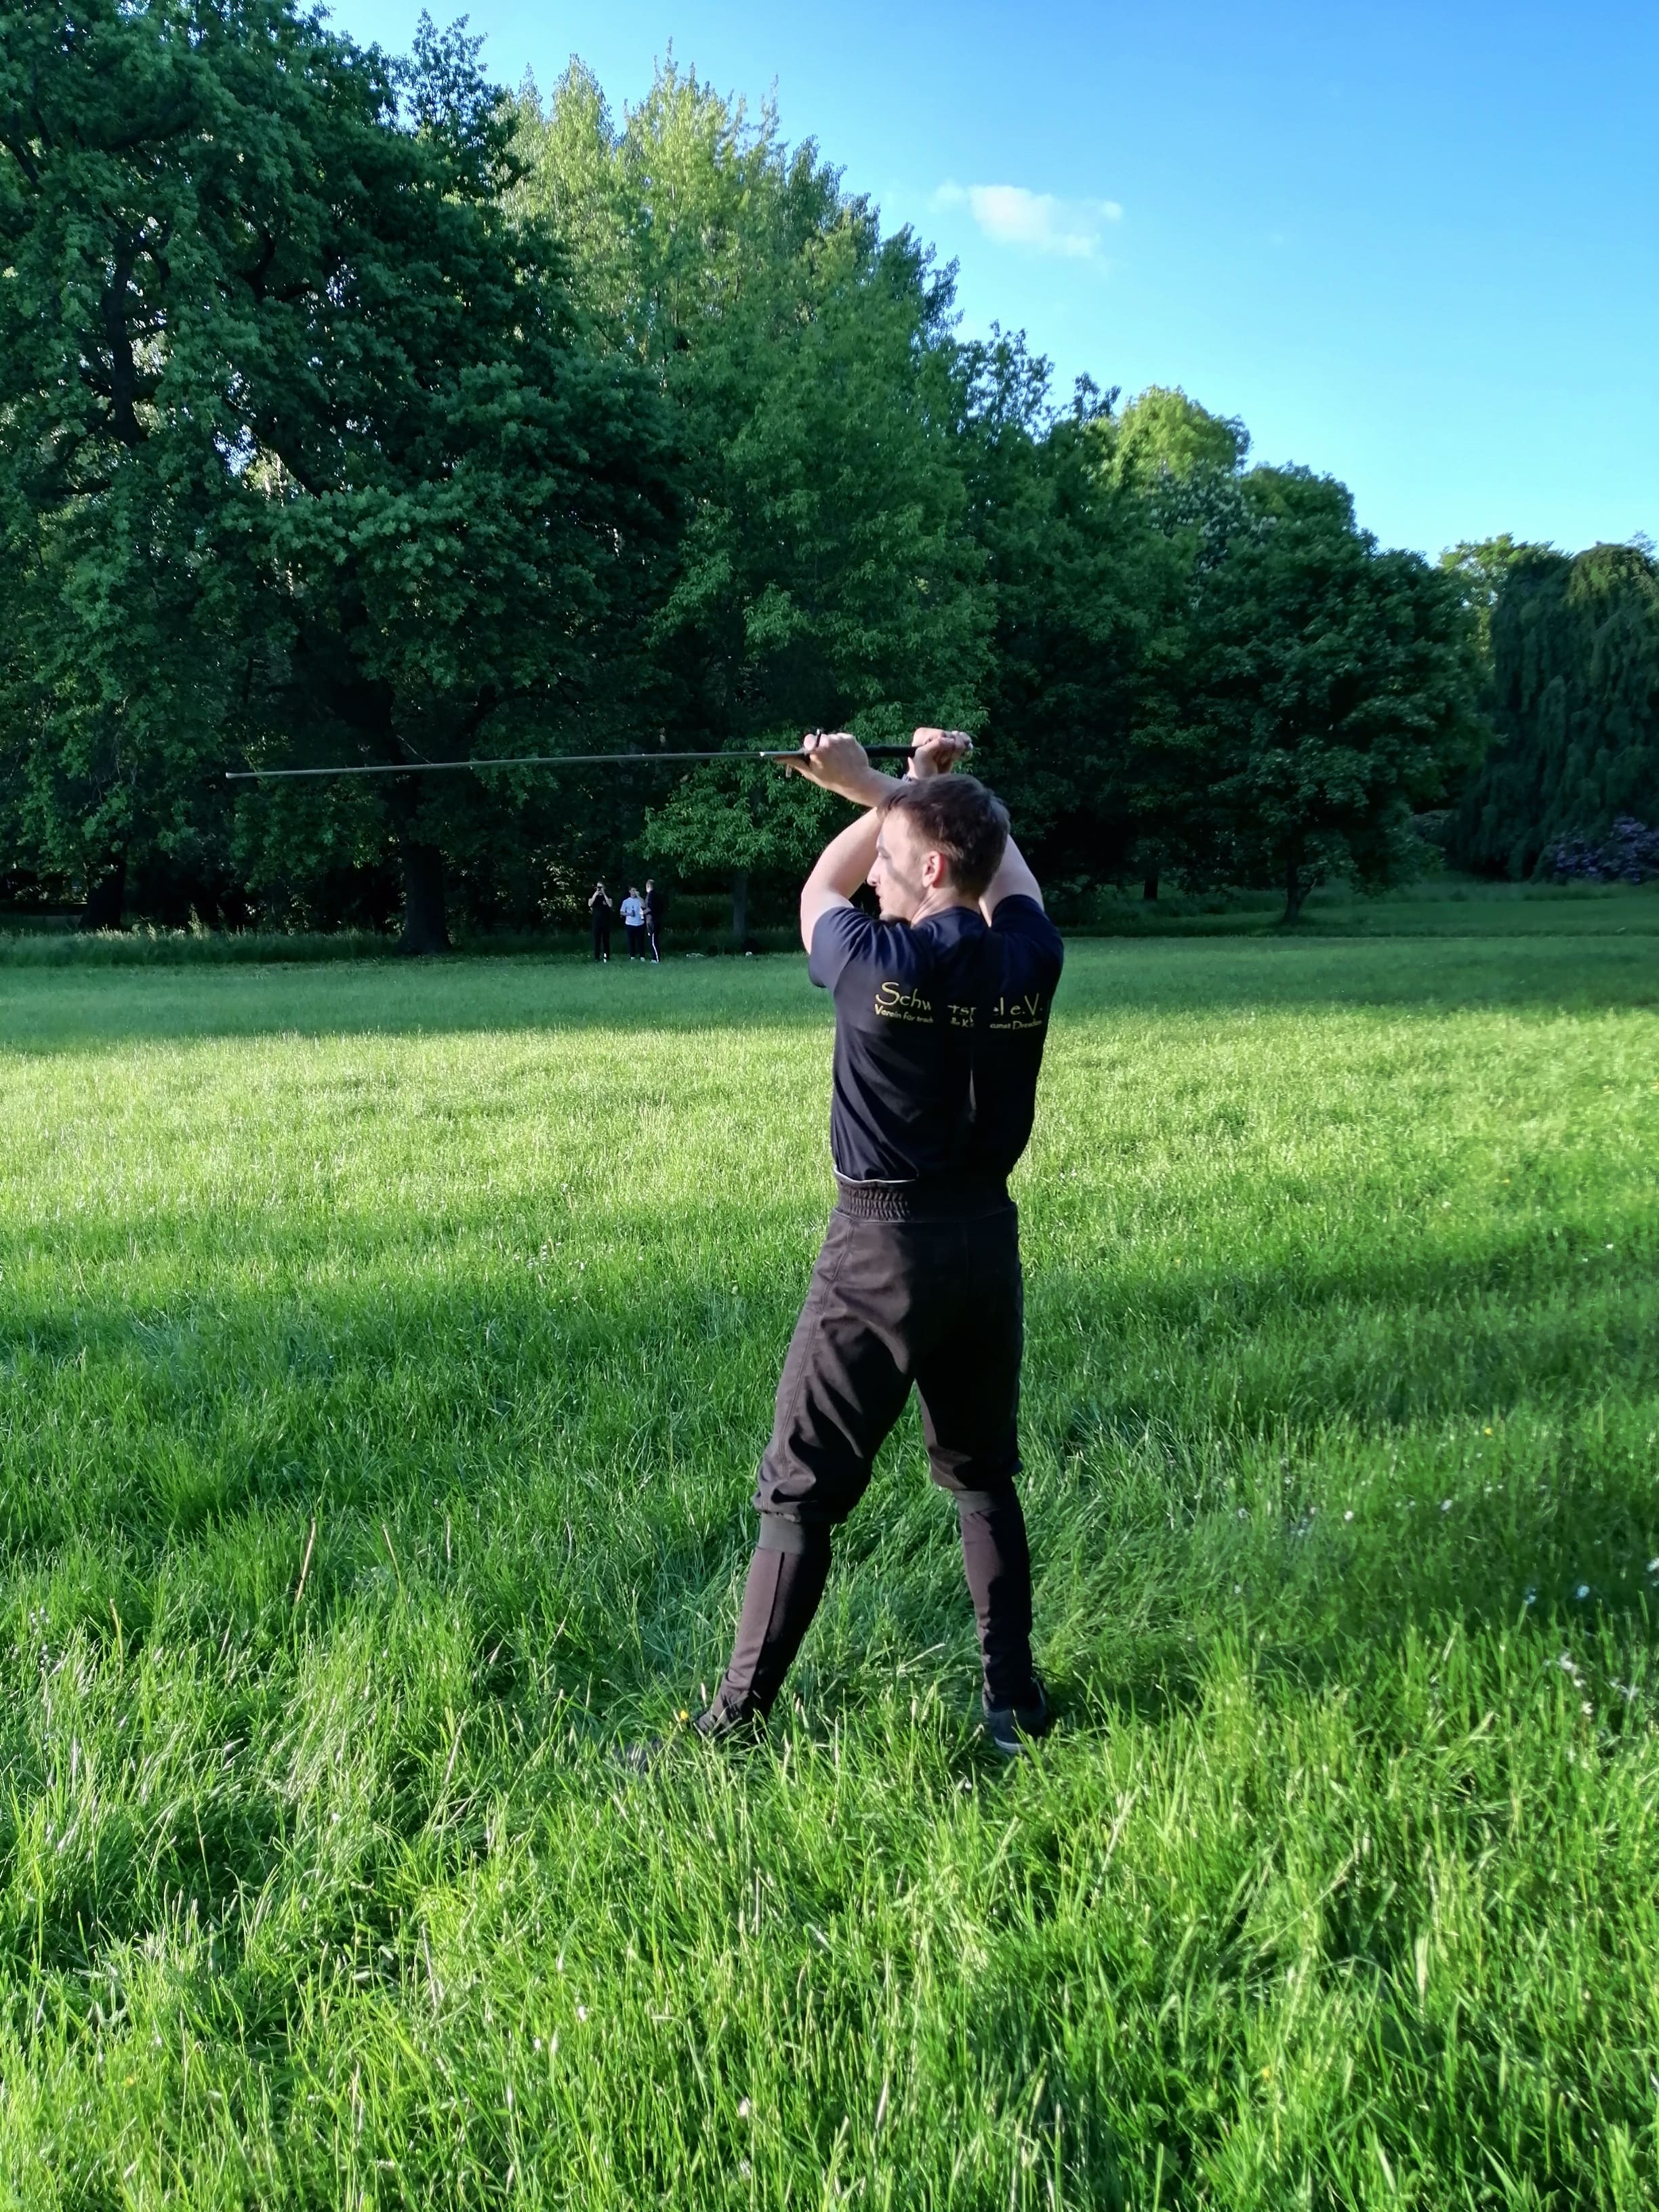
\includegraphics[width=\linewidth]{Ochs4.jpg}
  \caption{Ochs rechts}\label{fig:ochs4}
\endminipage\hfill
\minipage{0.32\textwidth}
  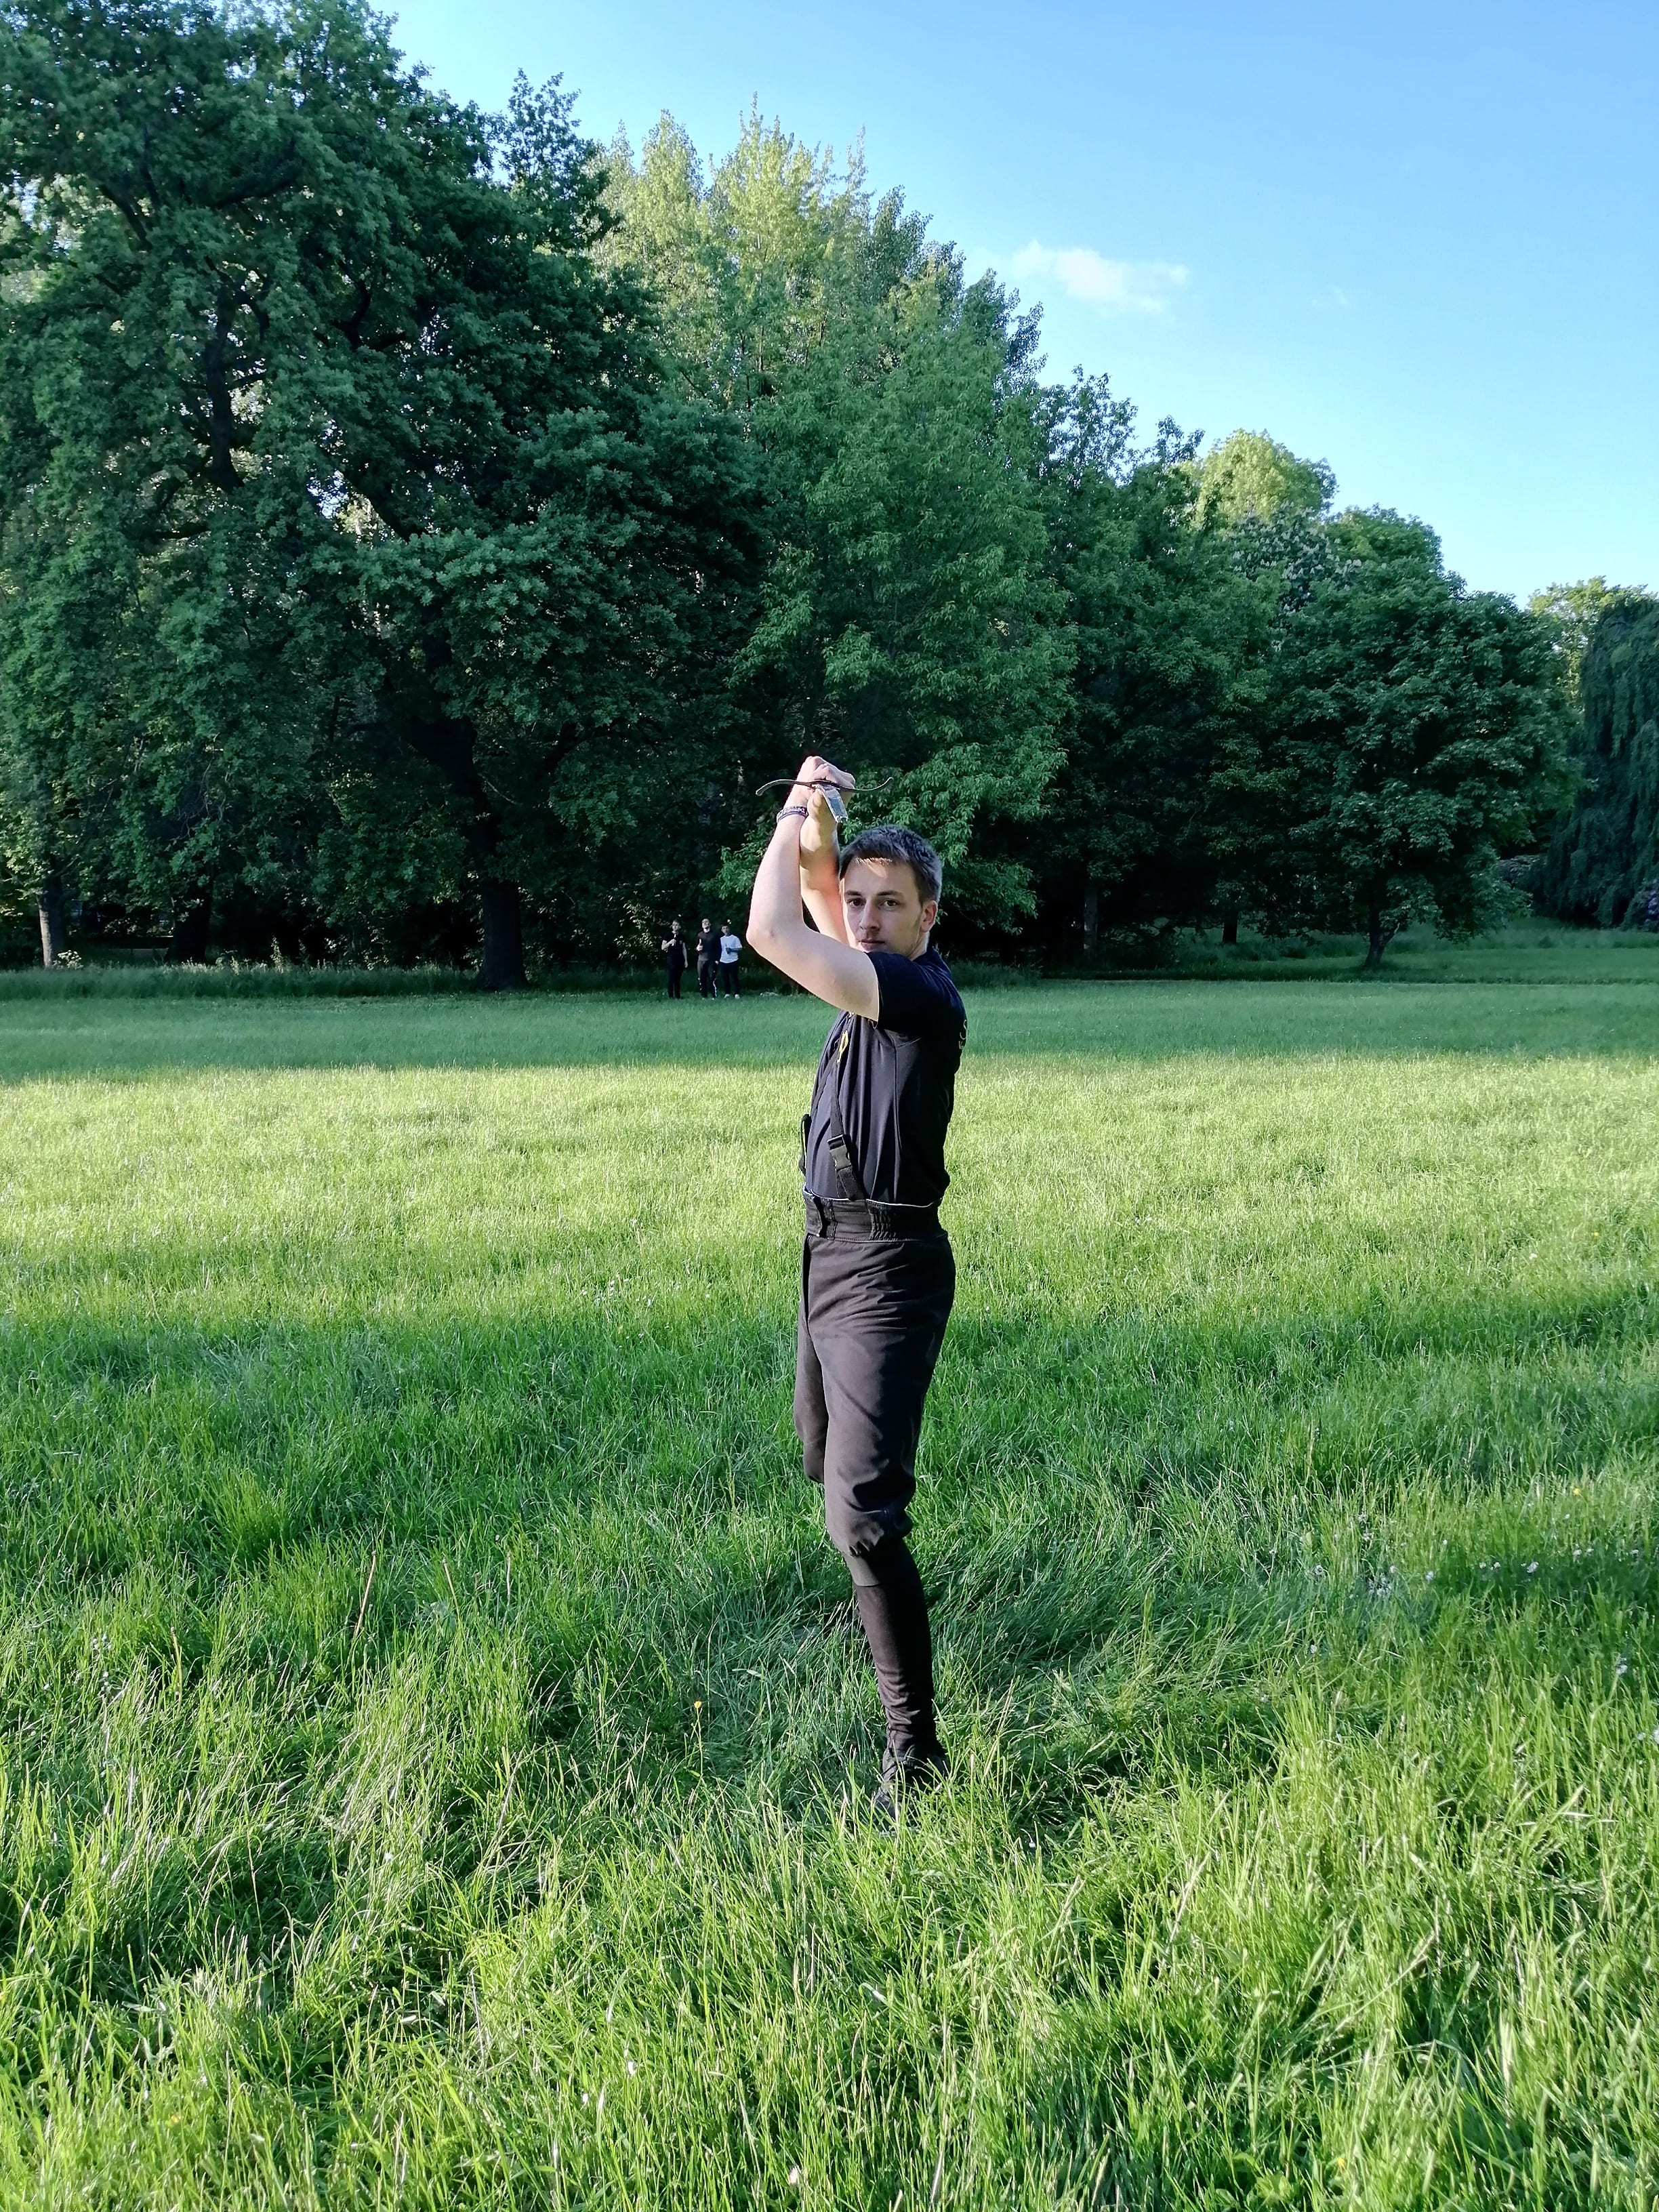
\includegraphics[width=\linewidth]{Ochs5.jpg}
  \caption{Ochs rechts}\label{fig:ochs5}
\endminipage\hfill
\minipage{0.32\textwidth}%
  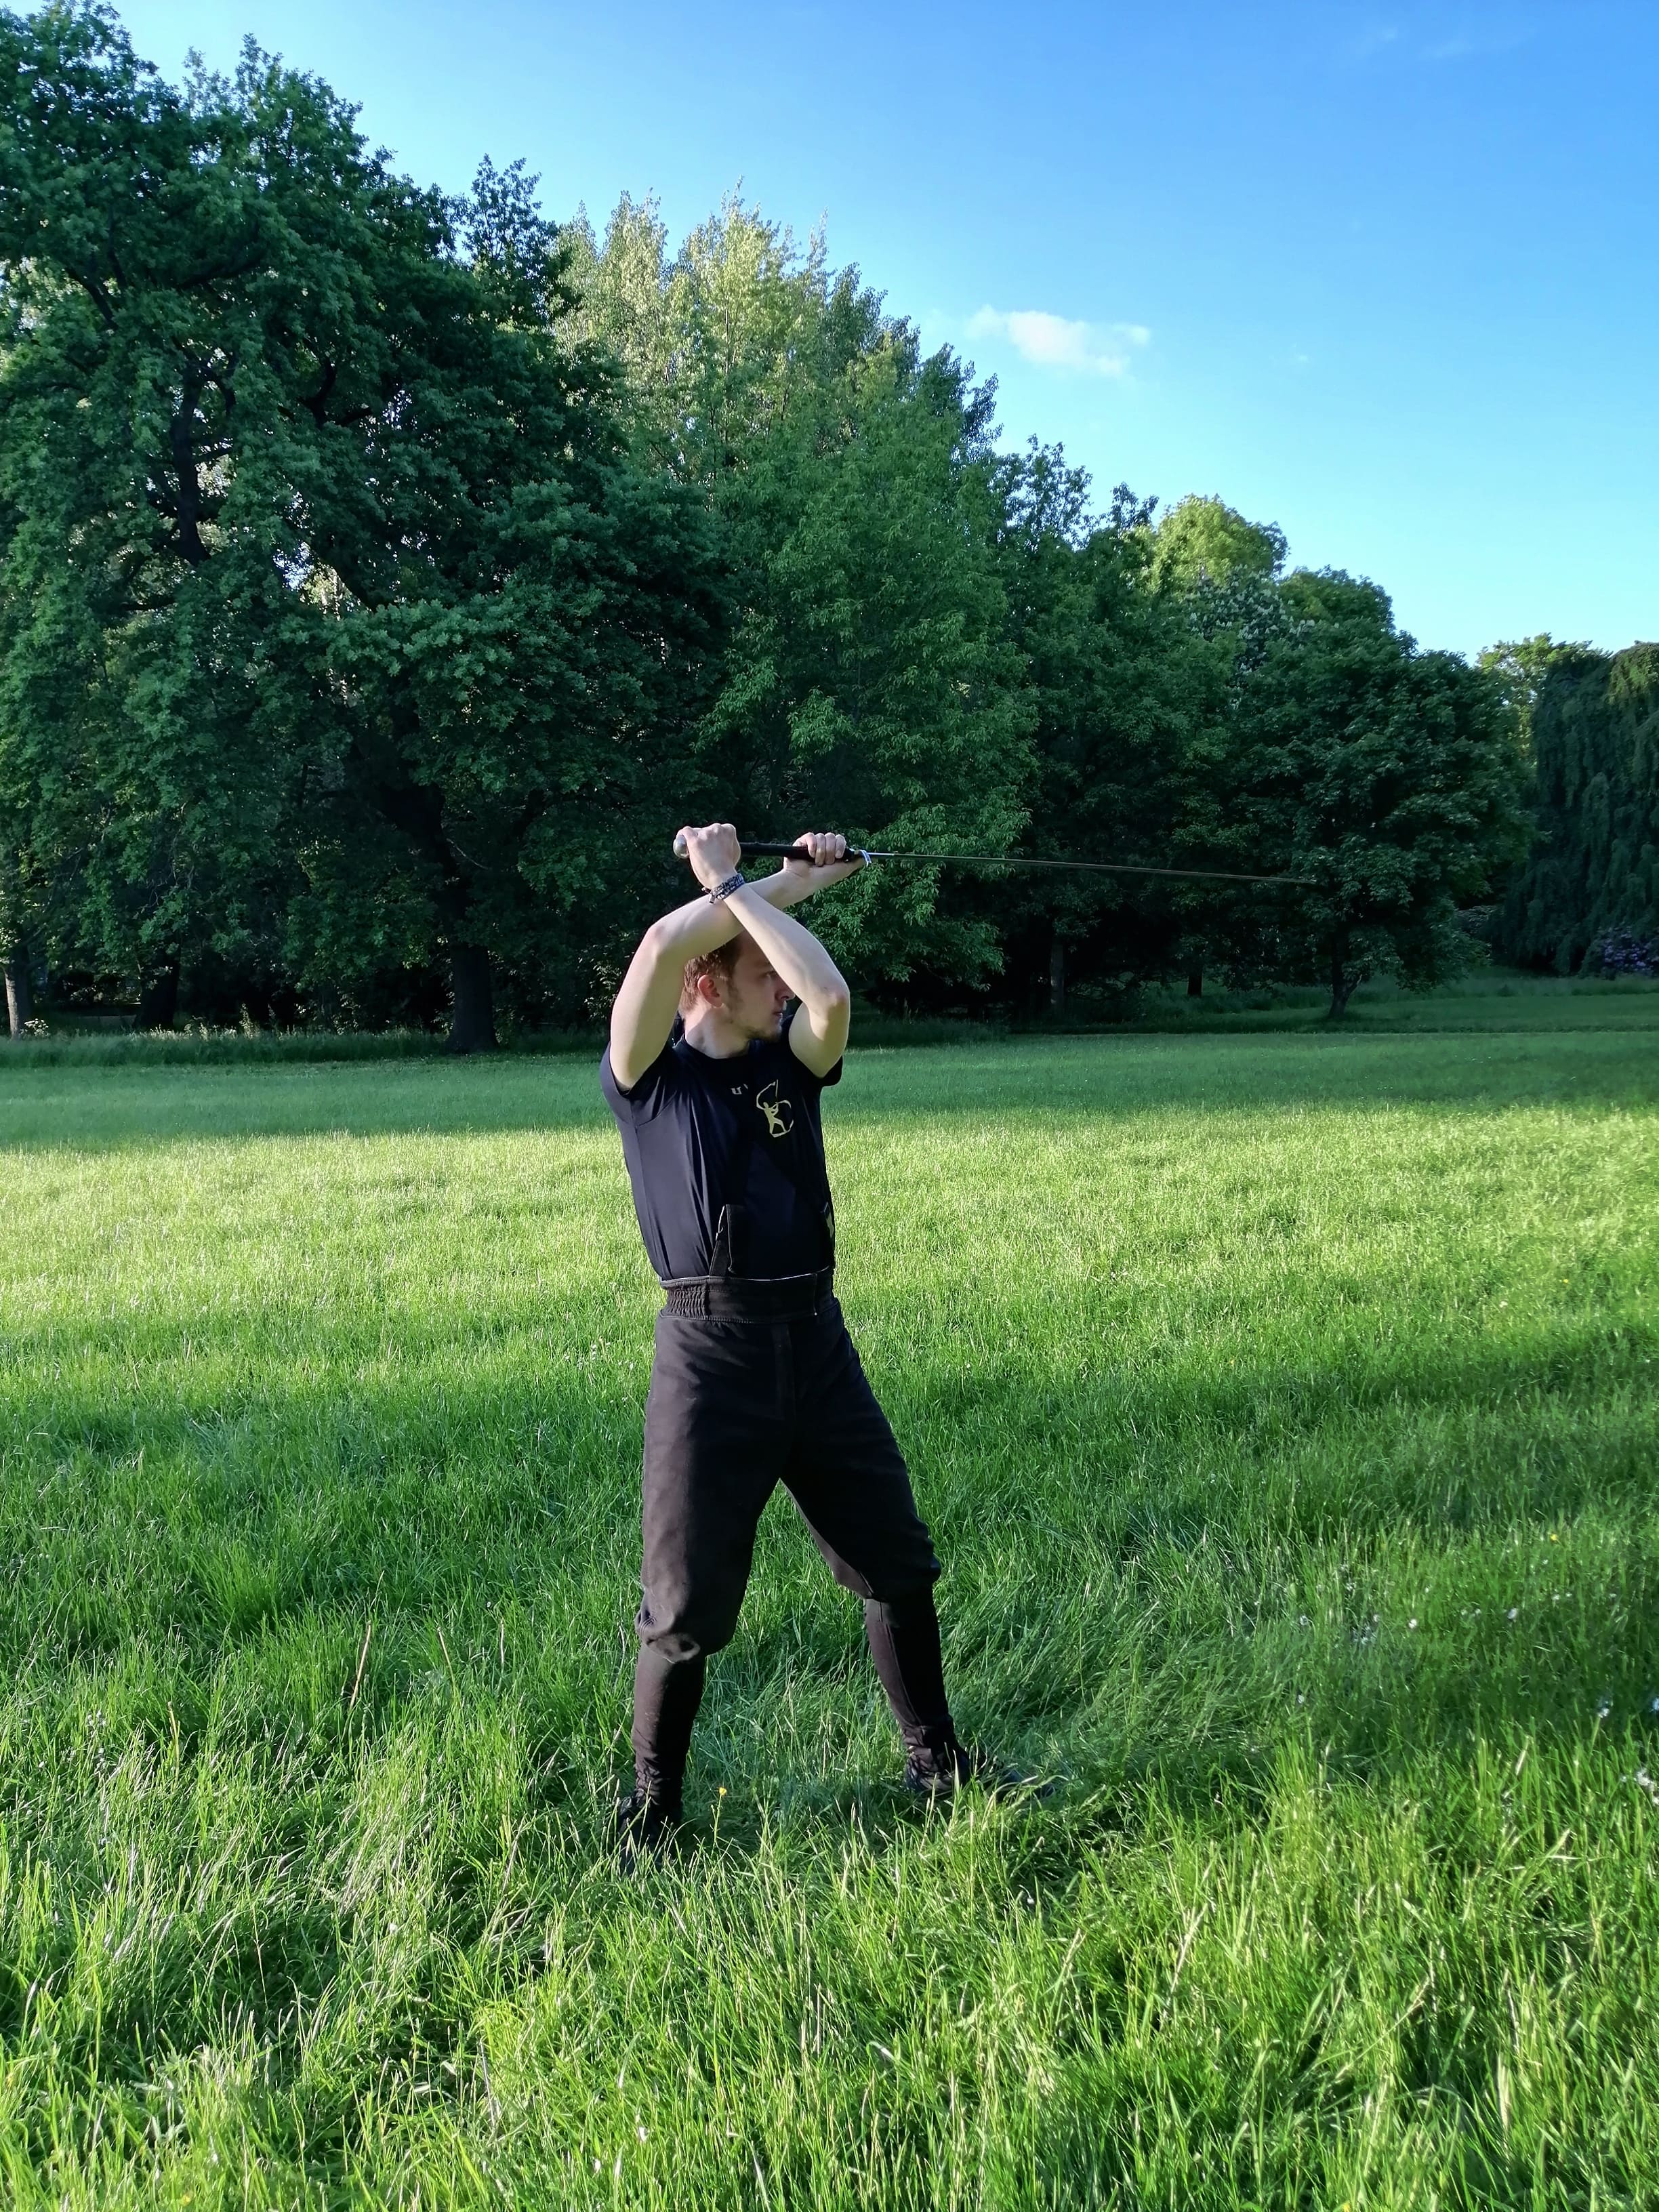
\includegraphics[width=\linewidth]{Ochs6.jpg}
  \caption{Ochs rechts}\label{fig:ochs6}
\endminipage
\end{figure}

Die Hut ''Ochs'' wird ebenfalls in links und rechts unterschieden. Die linke Seite unterscheidet sich von der Rechten in der Armhaltung: In der rechten Variante müssen (für Rechtshänder) die Arme gekreuzt werden, um das Schwert zu halten. Hierbei ist es wesentlich, dass die Handgelenke unter dem Schwert bleiben, um diese zu entlasten. Die Hände befinden sich etwas über Kopfhöhe. Der Ort ist zum Kopf oder Hals des Gegenübers gerichtet. Das Schwert wird im Daumengriff gehalten.

\newpage

\paragraph{Alber}

\begin{figure}[!ht]
\minipage{0.32\textwidth}
  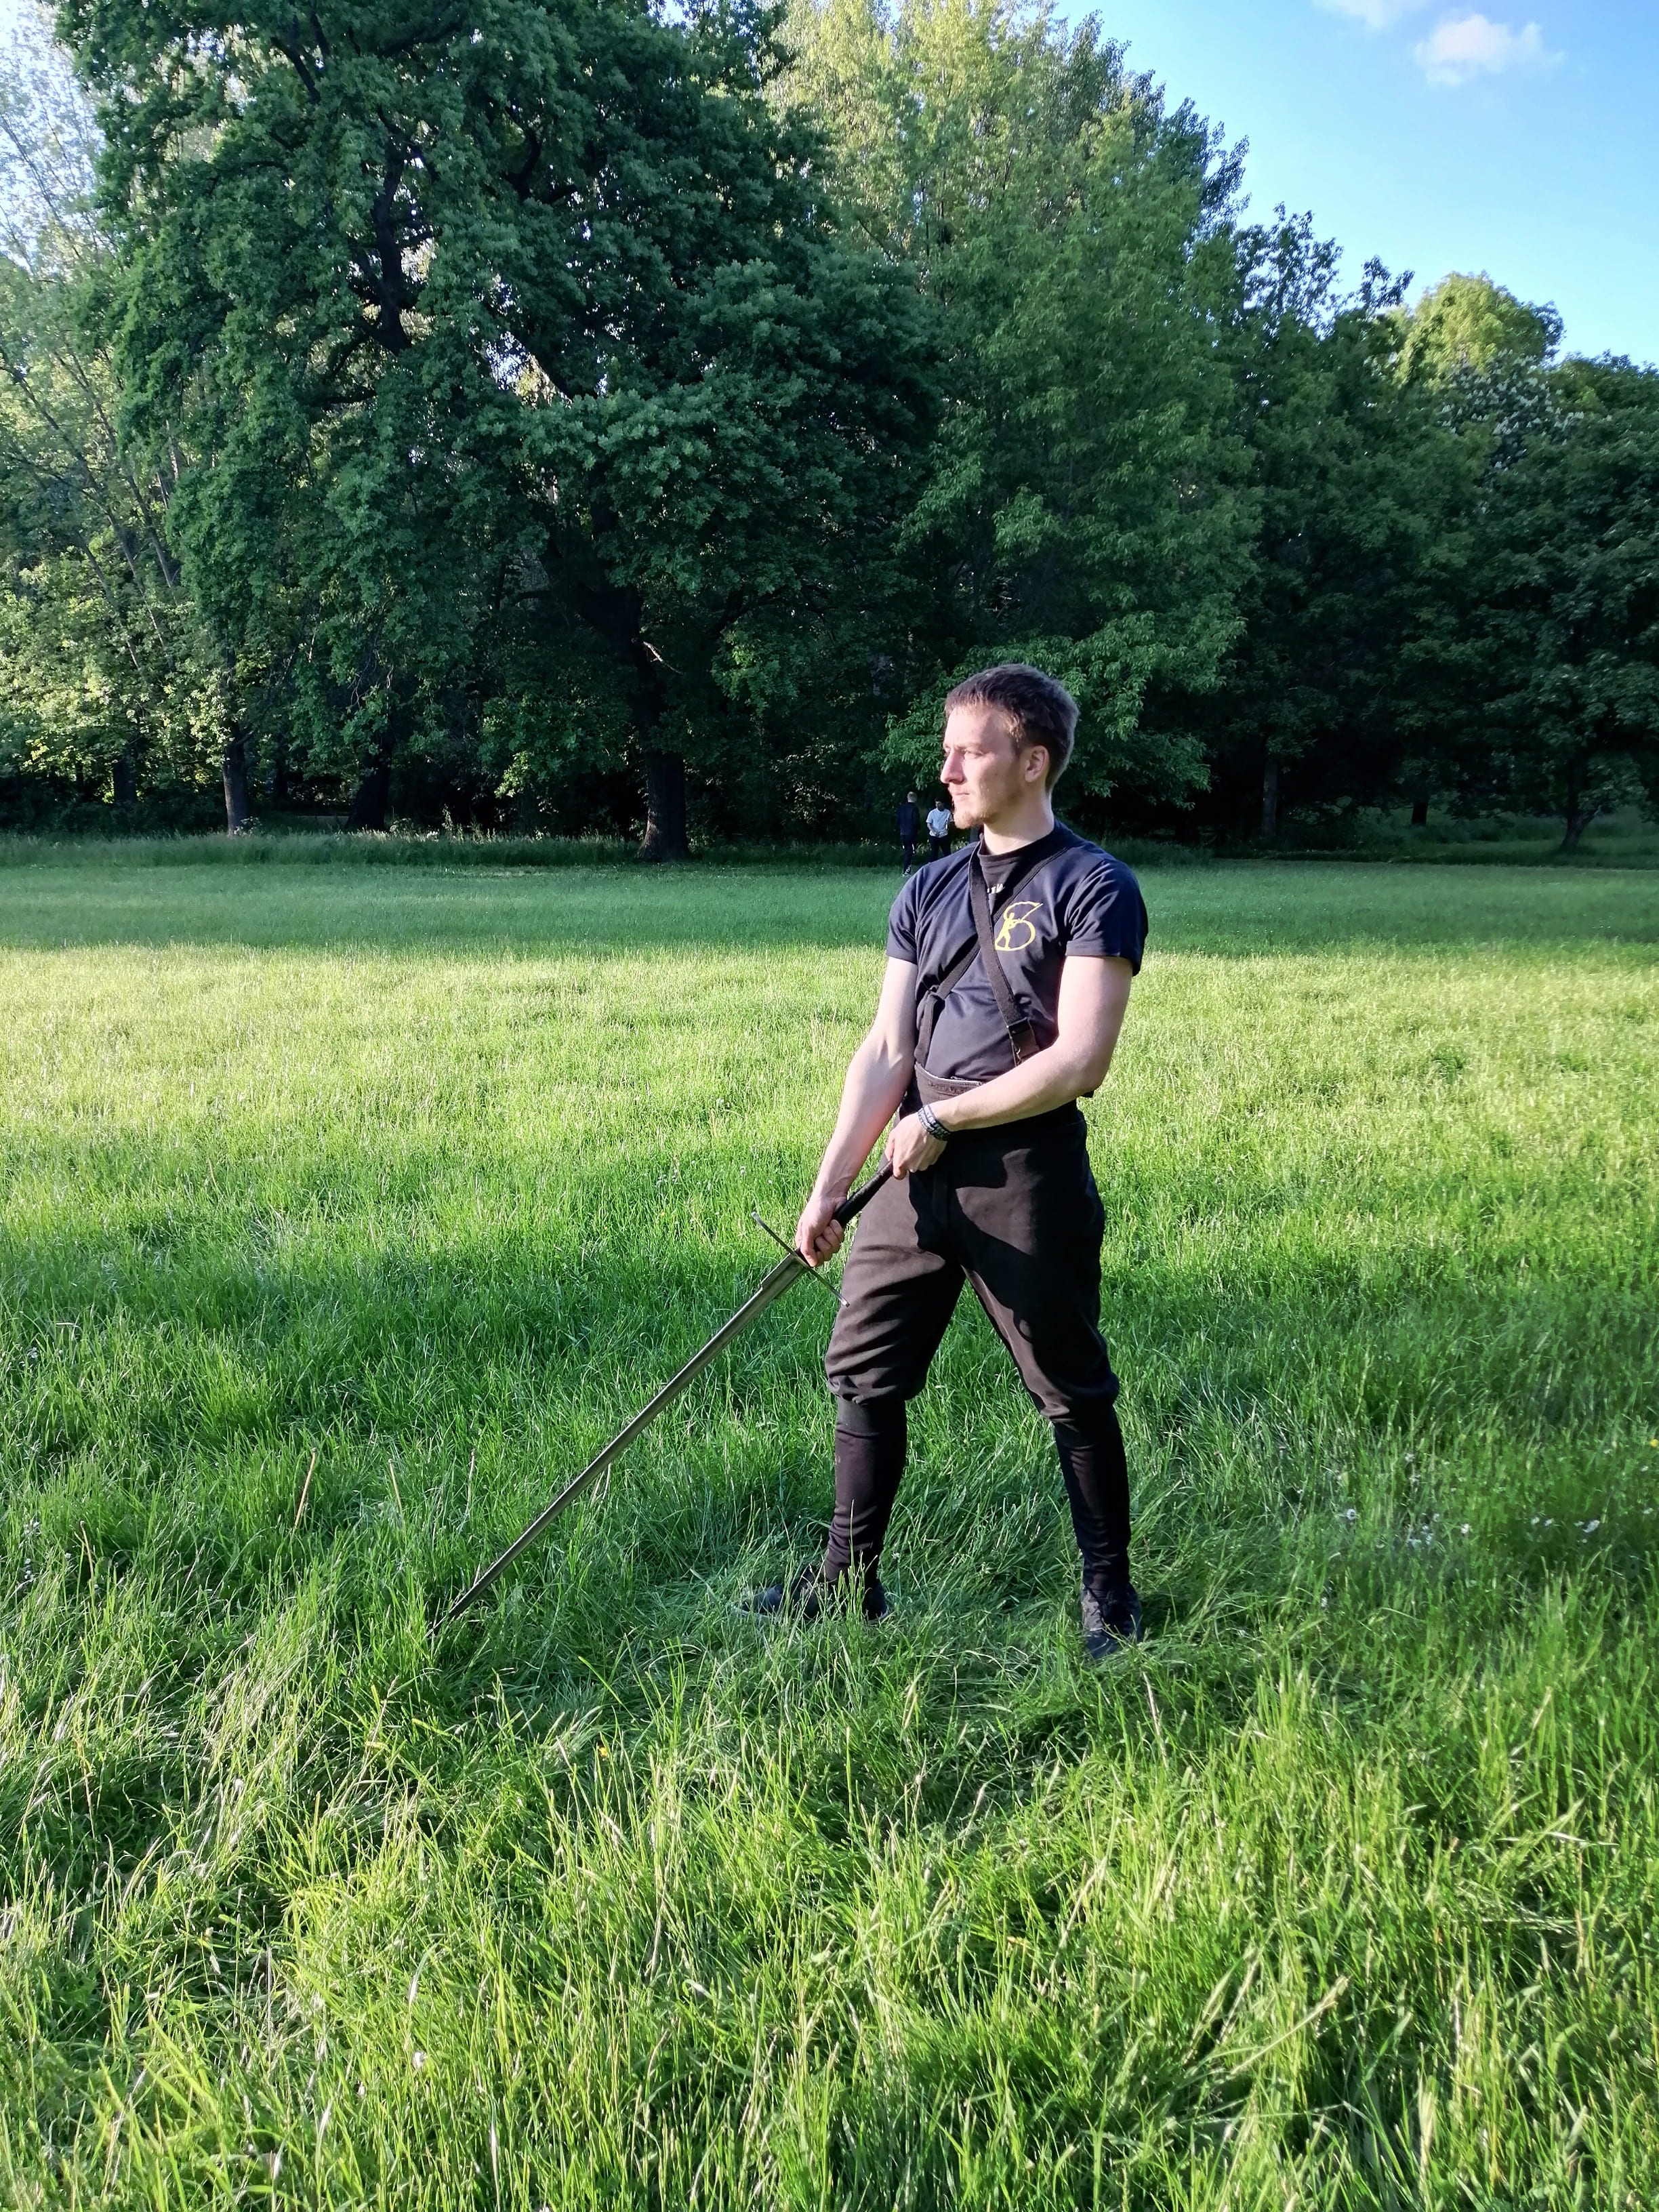
\includegraphics[width=\linewidth]{Alber1.jpg}
  \caption{links}\label{fig:alber1}
\endminipage\hfill
\minipage{0.32\textwidth}
  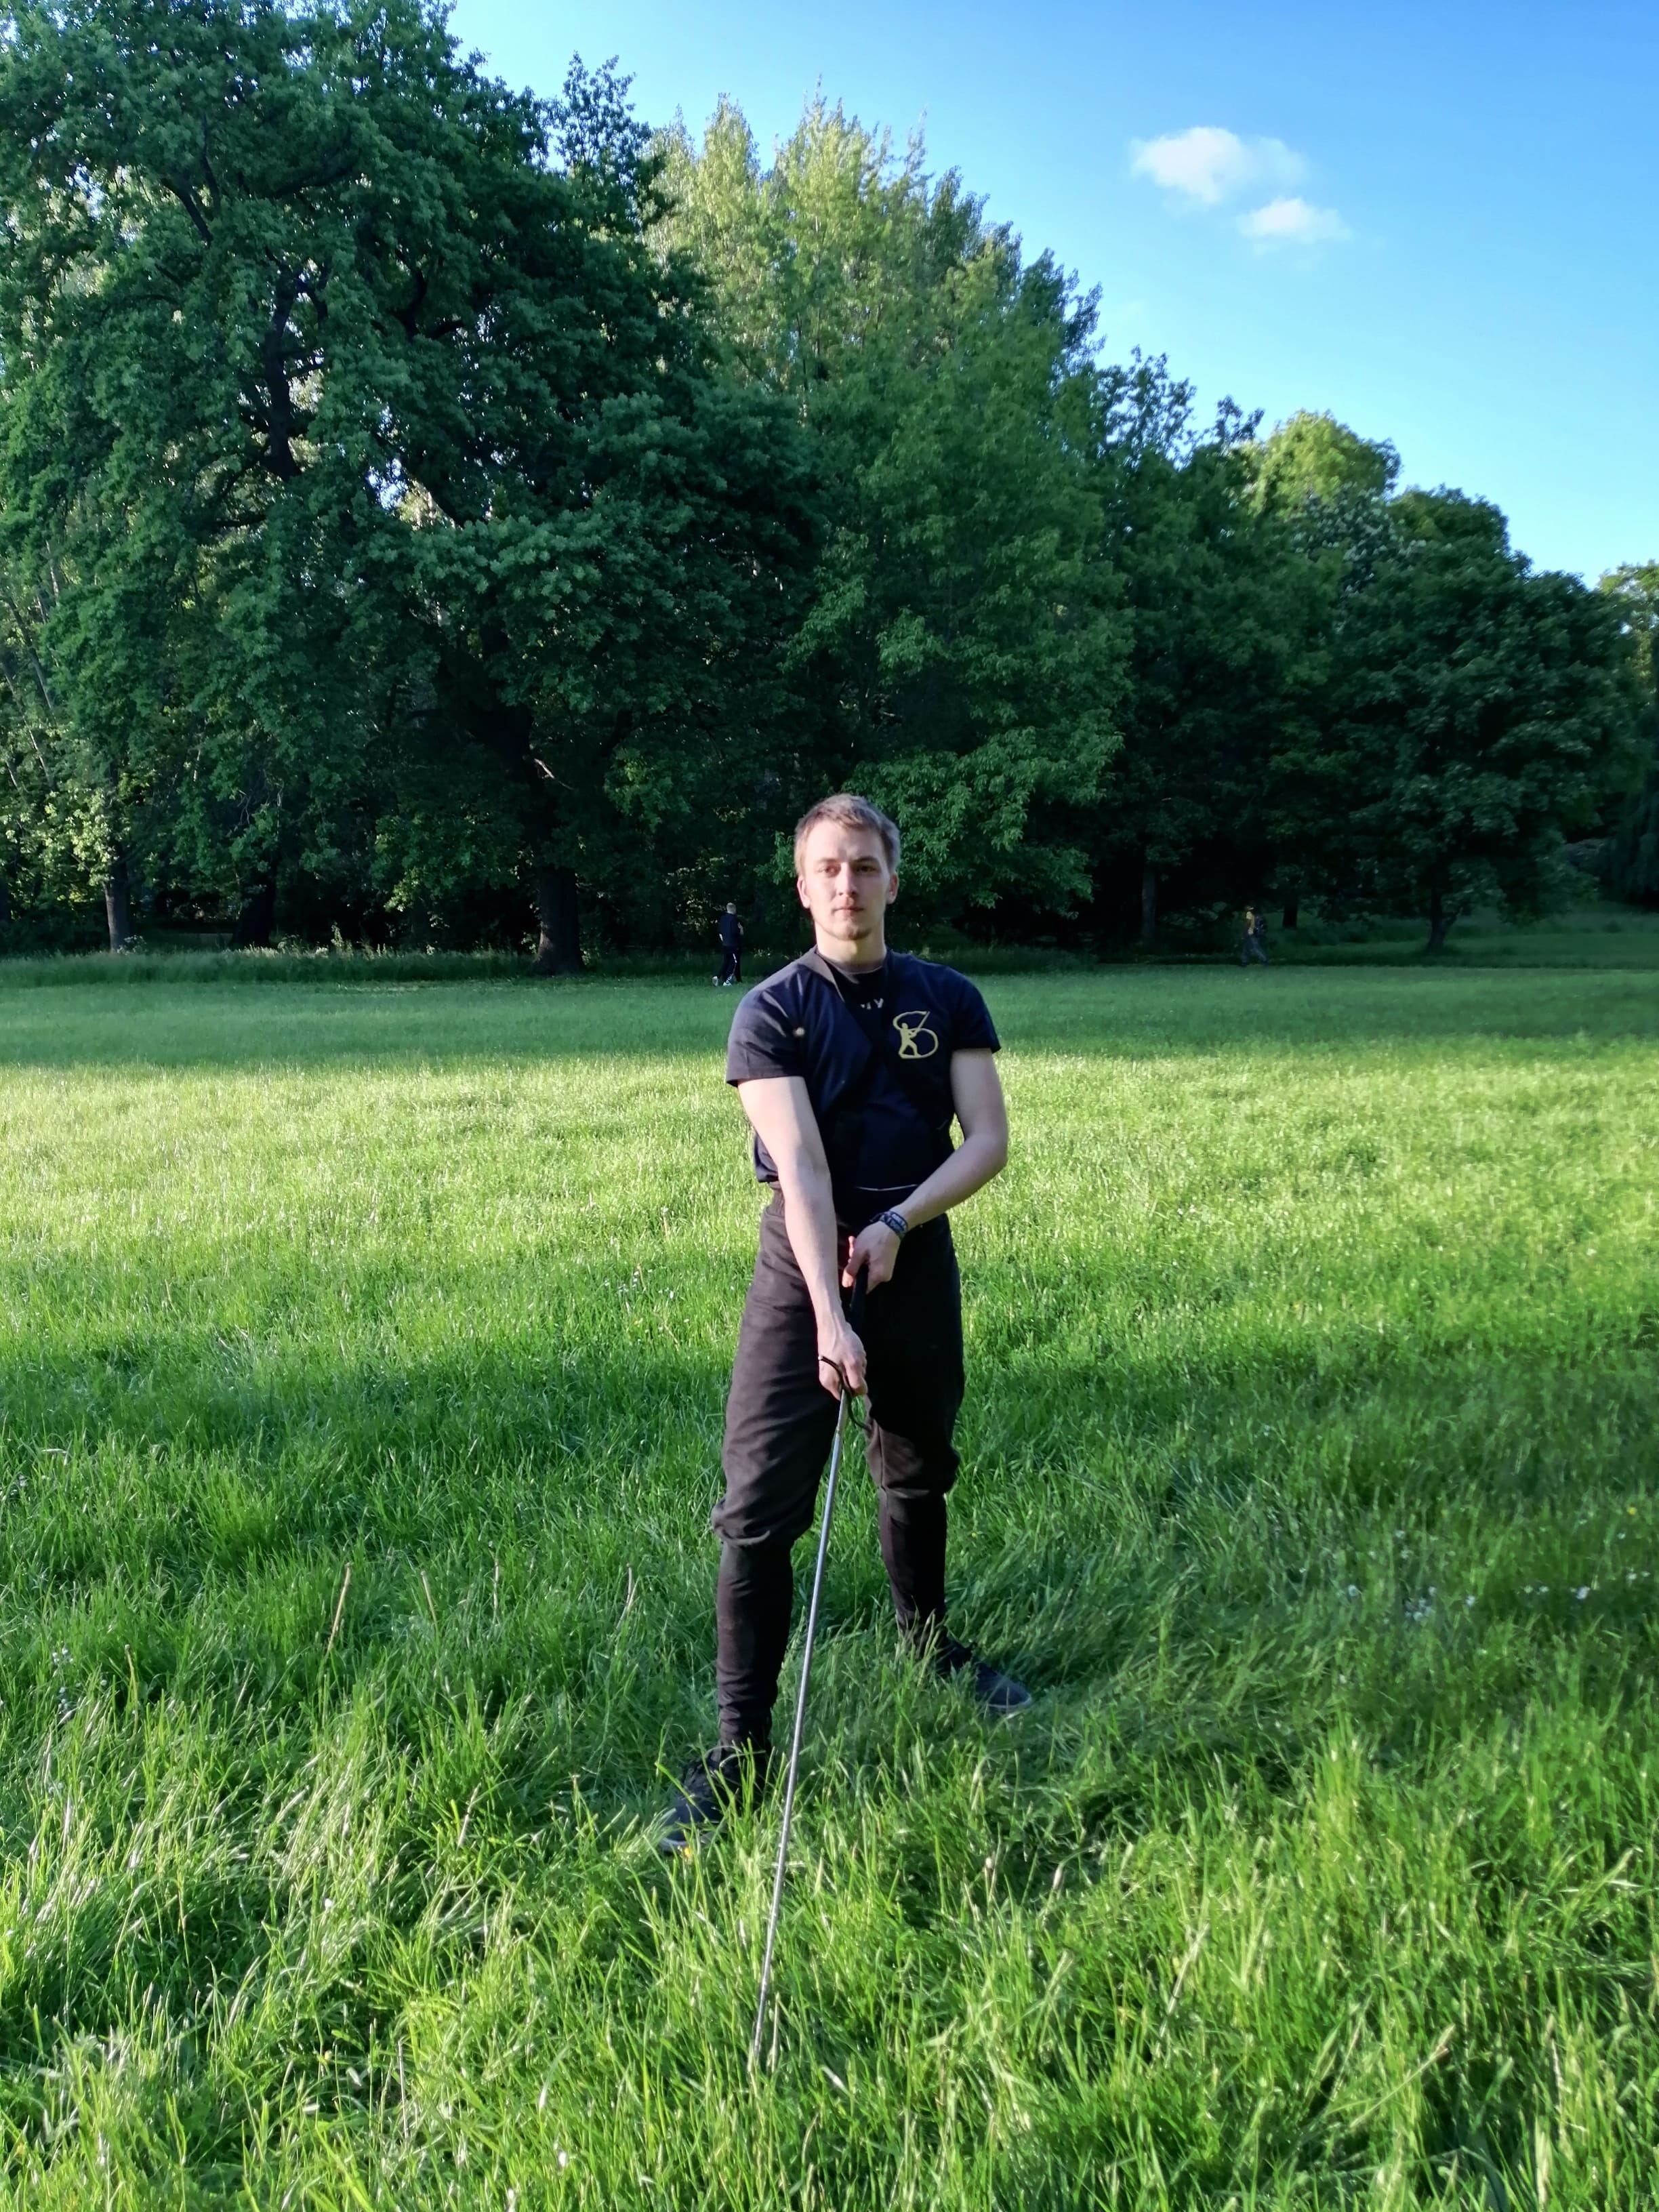
\includegraphics[width=\linewidth]{Alber2.jpg}
  \caption{frontal}\label{fig:alber2}
\endminipage\hfill
\minipage{0.32\textwidth}%
  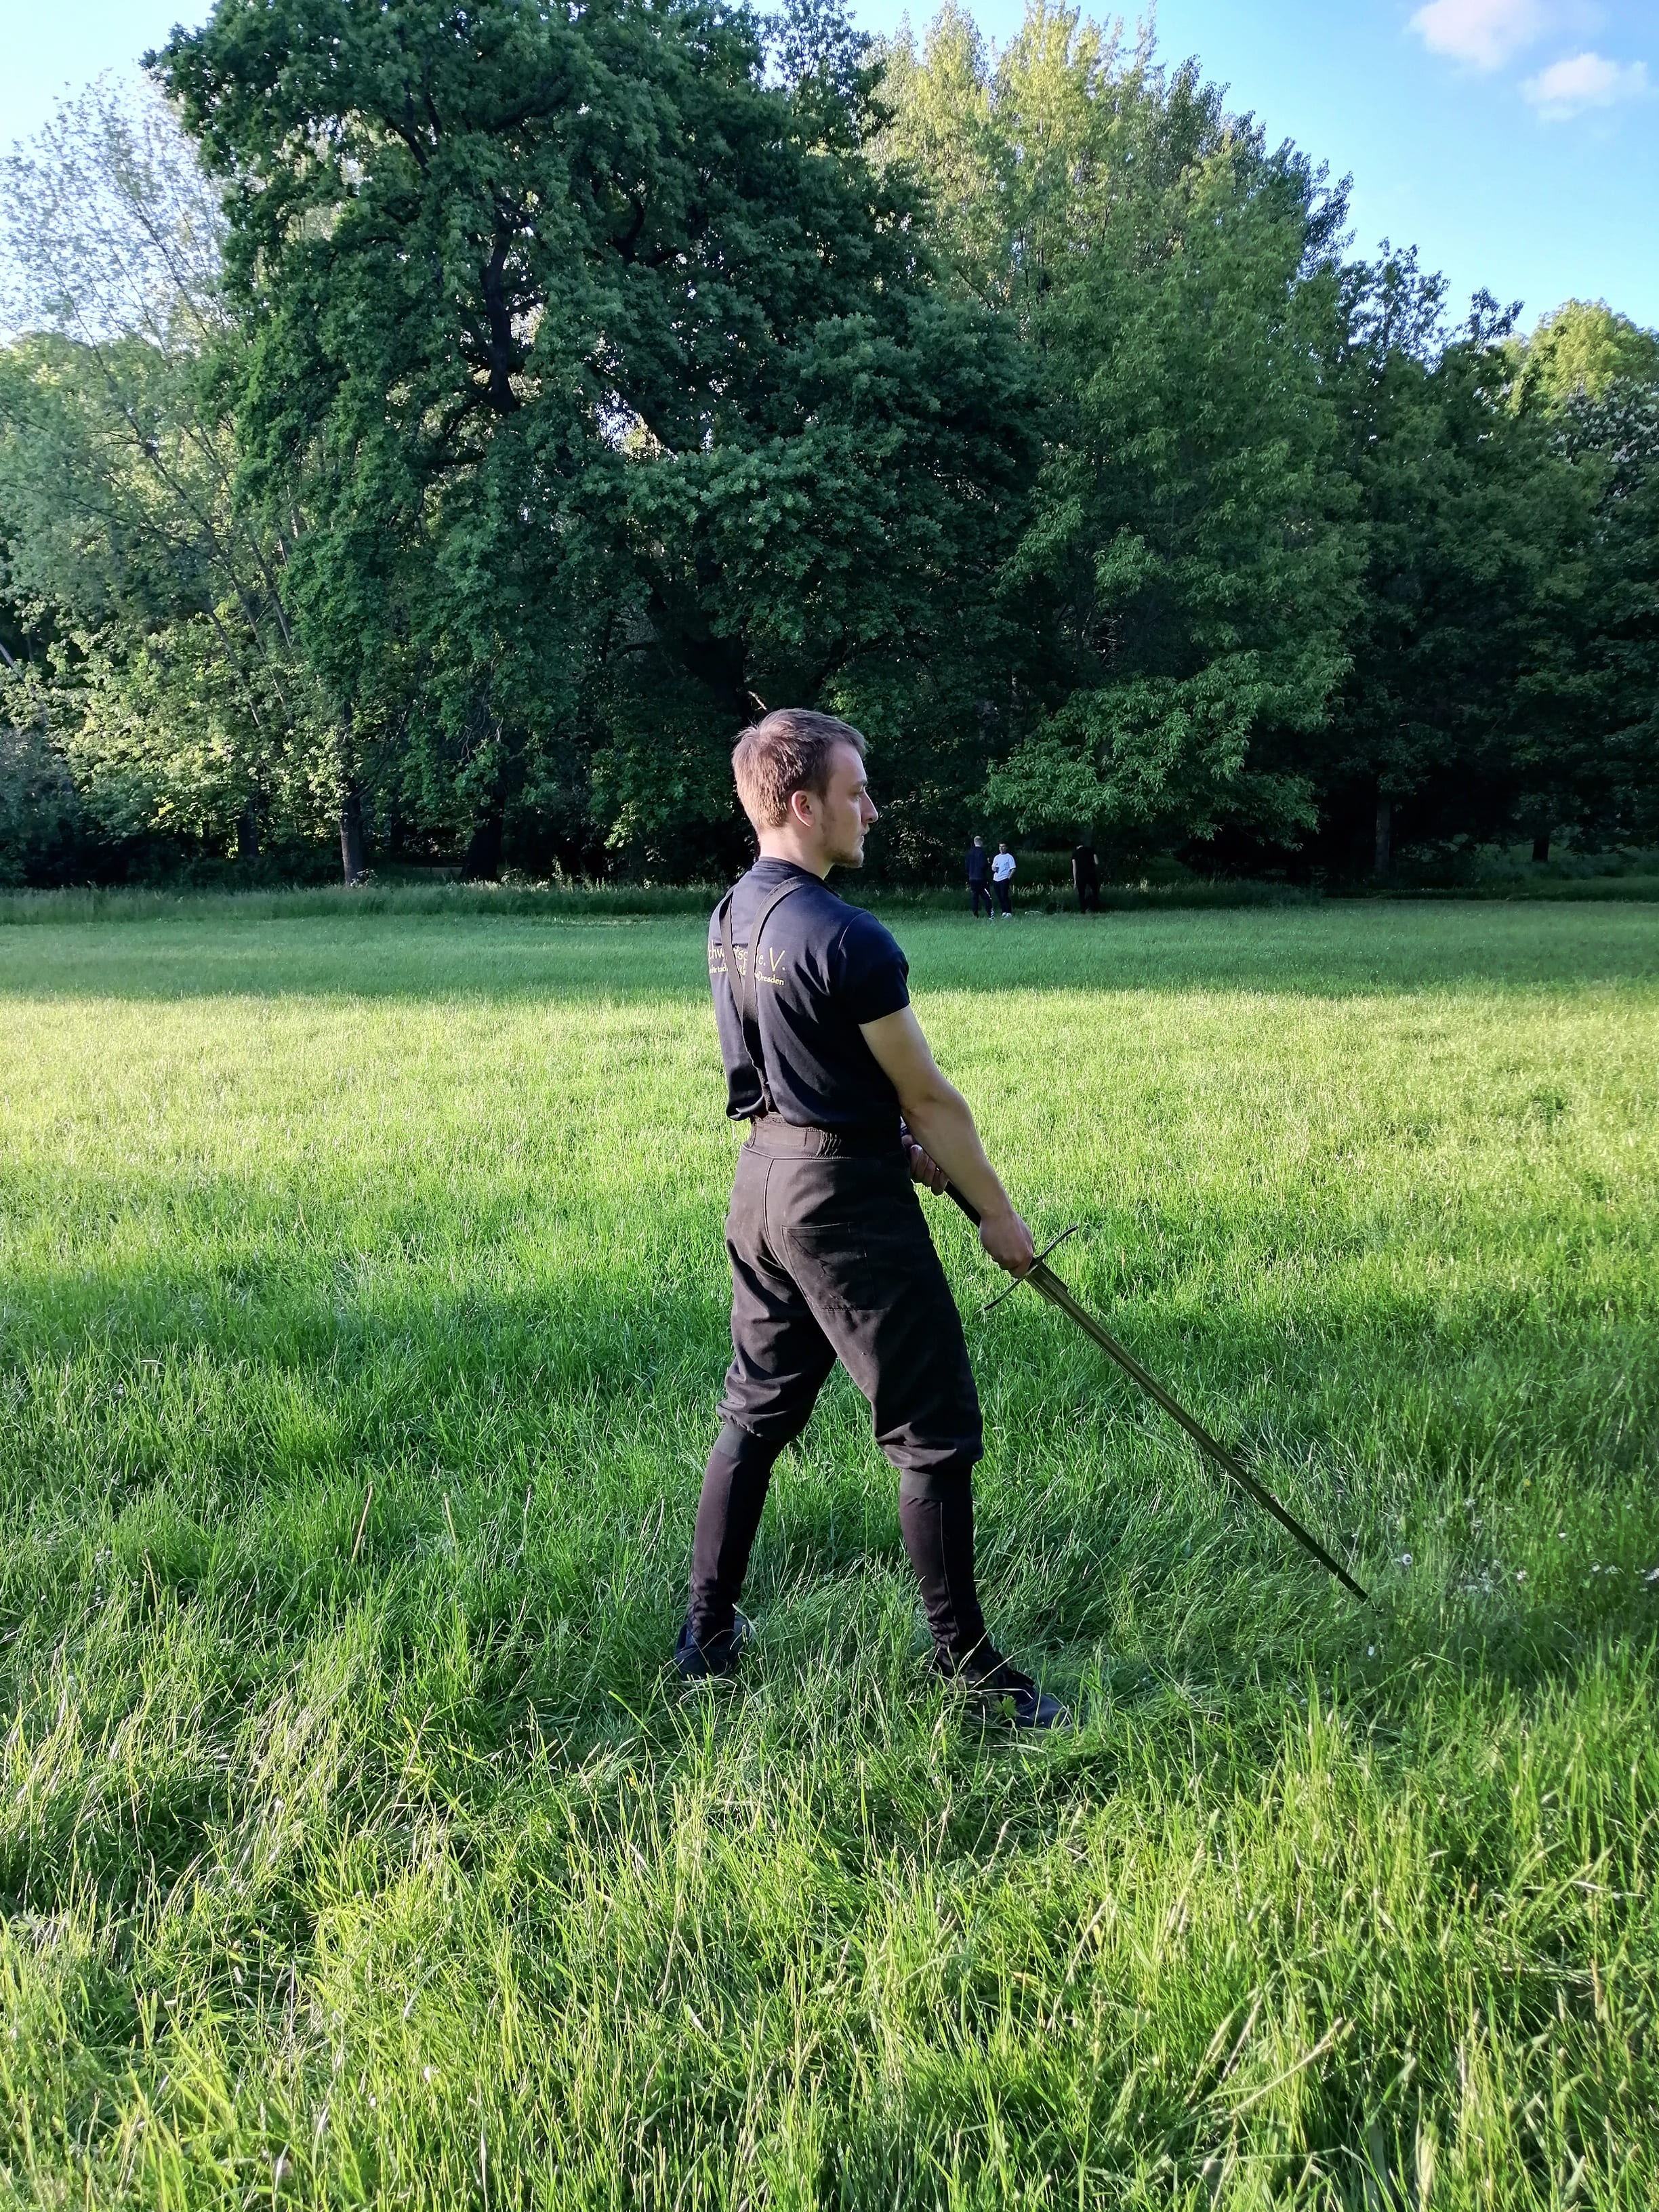
\includegraphics[width=\linewidth]{Alber3.jpg}
  \caption{rechts}\label{fig:alber3}
\endminipage
\end{figure}

Die Hut ''Alber'' kennt nur die neutrale Position. Daher kann die Fußstellung frei gewählt werden. Es empfiehlt sich, vorausschauend eine Fußstellung und Griffweise so zu wählen, dass sie die geplante Aktion unterstützen.
\\
\FloatBarrier
\hrule

\begin{figure}[!ht]
\minipage{0.5\textwidth}
  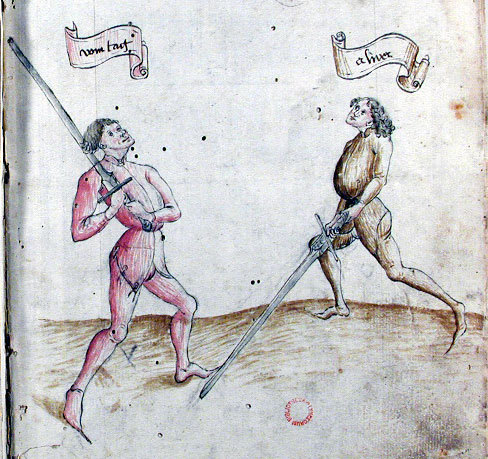
\includegraphics[width=\linewidth]{Haupthuten1.jpg}
  \caption{Vom Tag und Alber}\label{fig:haupthuten1}
\endminipage\hfill
\minipage{0.4\textwidth}
  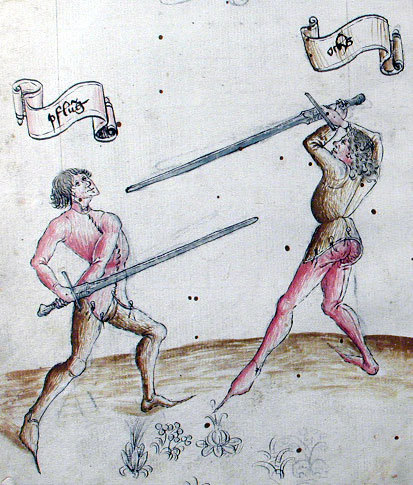
\includegraphics[width=\linewidth]{Haupthuten2.jpg}
  \caption{Ochs und Pflug}\label{fig:haupthuten2}
\endminipage\hfill
\end{figure}

\FloatBarrier

Die Darstellung der Huten im Codex 44 A 8, 1452

\newpage

\subsubsection{Blößen}

Das finale Ziel aller Aktionen im Fechten sollte es sein, das Gegenüber zu treffen, ohne dabei selbst getroffen zu werden. Dazu entstand sowohl in der italienischen, als auch in der deutschen Fechtart das Prinzip der ''Blößen''. Die Blößen beschreiben potentielle Ziele, welche nicht durch das Schwert geschützt werden. Das Wissen über die eigenen Blößen, die Blößen des Gegenübers und wie diese möglichst effizient zu schützen, bzw. zu erreichen sind, ist deshalb essentiell für alle Entscheidungen in einem Gefecht.
\\
\\
In einem Dresdner Manuskript\footnote{\hspace*{0.5ex}Dresden, SLUB, Mscr.Dresd.C.487, fol. 22v-23r, eigene Transkription und Übersetzung.} steht dazu:
\\
\\
(22v) Vier Blößen wisse zu nehmen, so schlägst Du gewisse, alle Vier. Ohne Zweifel, (egal) wie er sich gebärdet.
\\
\\
(22v-23r) Hier sollst Du Dir die vier Blößen an dem Mann merken, dass Du diesen immer zufechten sollst. Die erste Blöße ist die rechte Seite, die Andere ist die linke Seite, oberhalb des Gürtels des Mannes.
\\
\\
Die anderen Zwei sind die rechte und die linke Seite unterhalb des Gürtels. Diese Blößen nehmen eben wahr, in dem Zufechten. Mit welcher Blöße er sich gegen Dich entblößt. Diese greife künstlich ohne Gefahr an. Mit dem Einschießen des Langen Ortes, mit Nachreisen und sonst mit allen Gefechten. Und achte nicht darauf, wie er sich mit seinen Gefechten gegen Dich verhält.So fechtest Du sicher und schlägst Schläge daraus, die sehr trefflich sind und lässt ihn damit nicht zu seinen Stücken kommen.''

\begin{figure}
    \centering
    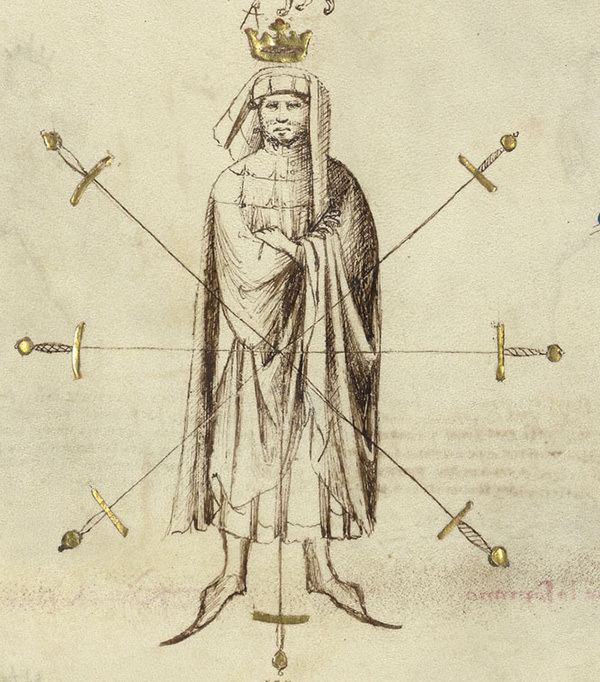
\includegraphics[scale=.27]{fiore-dei-liberi.jpeg}
    \caption{Darstellung der Blößen, ''Fior di Battaglia'' (MS Ludwig XV 13, 1404)}
    \label{fig:Blößen}
\end{figure}
   
% Quelle http://fechtfabrik.de/fiore-dei-liberi/
% unter  CopyLeft Lizenz 

\FloatBarrier

\newpage

\subsubsection{Mensur}

Der Abstand zum:zur Gegner:in wird allgemein als ''Mensur'' bezeichnet. Bestimmte Techniken erfordern eine bestimmte Mensur. Die Fähigkeit, Mensur einzuschätzen, sowie das Wissen darüber, welche Technik in welcher Situation optimal ist, sind Schlüssel zum erfolgreichen Fechten. Sie erlauben es, erfolgreich die Initiative zu ergreifen und machen das Gefecht berechenbarer.

\paragraph{Zufechtmensur}

\FloatBarrier

\begin{figure}[!ht]
    \centering
    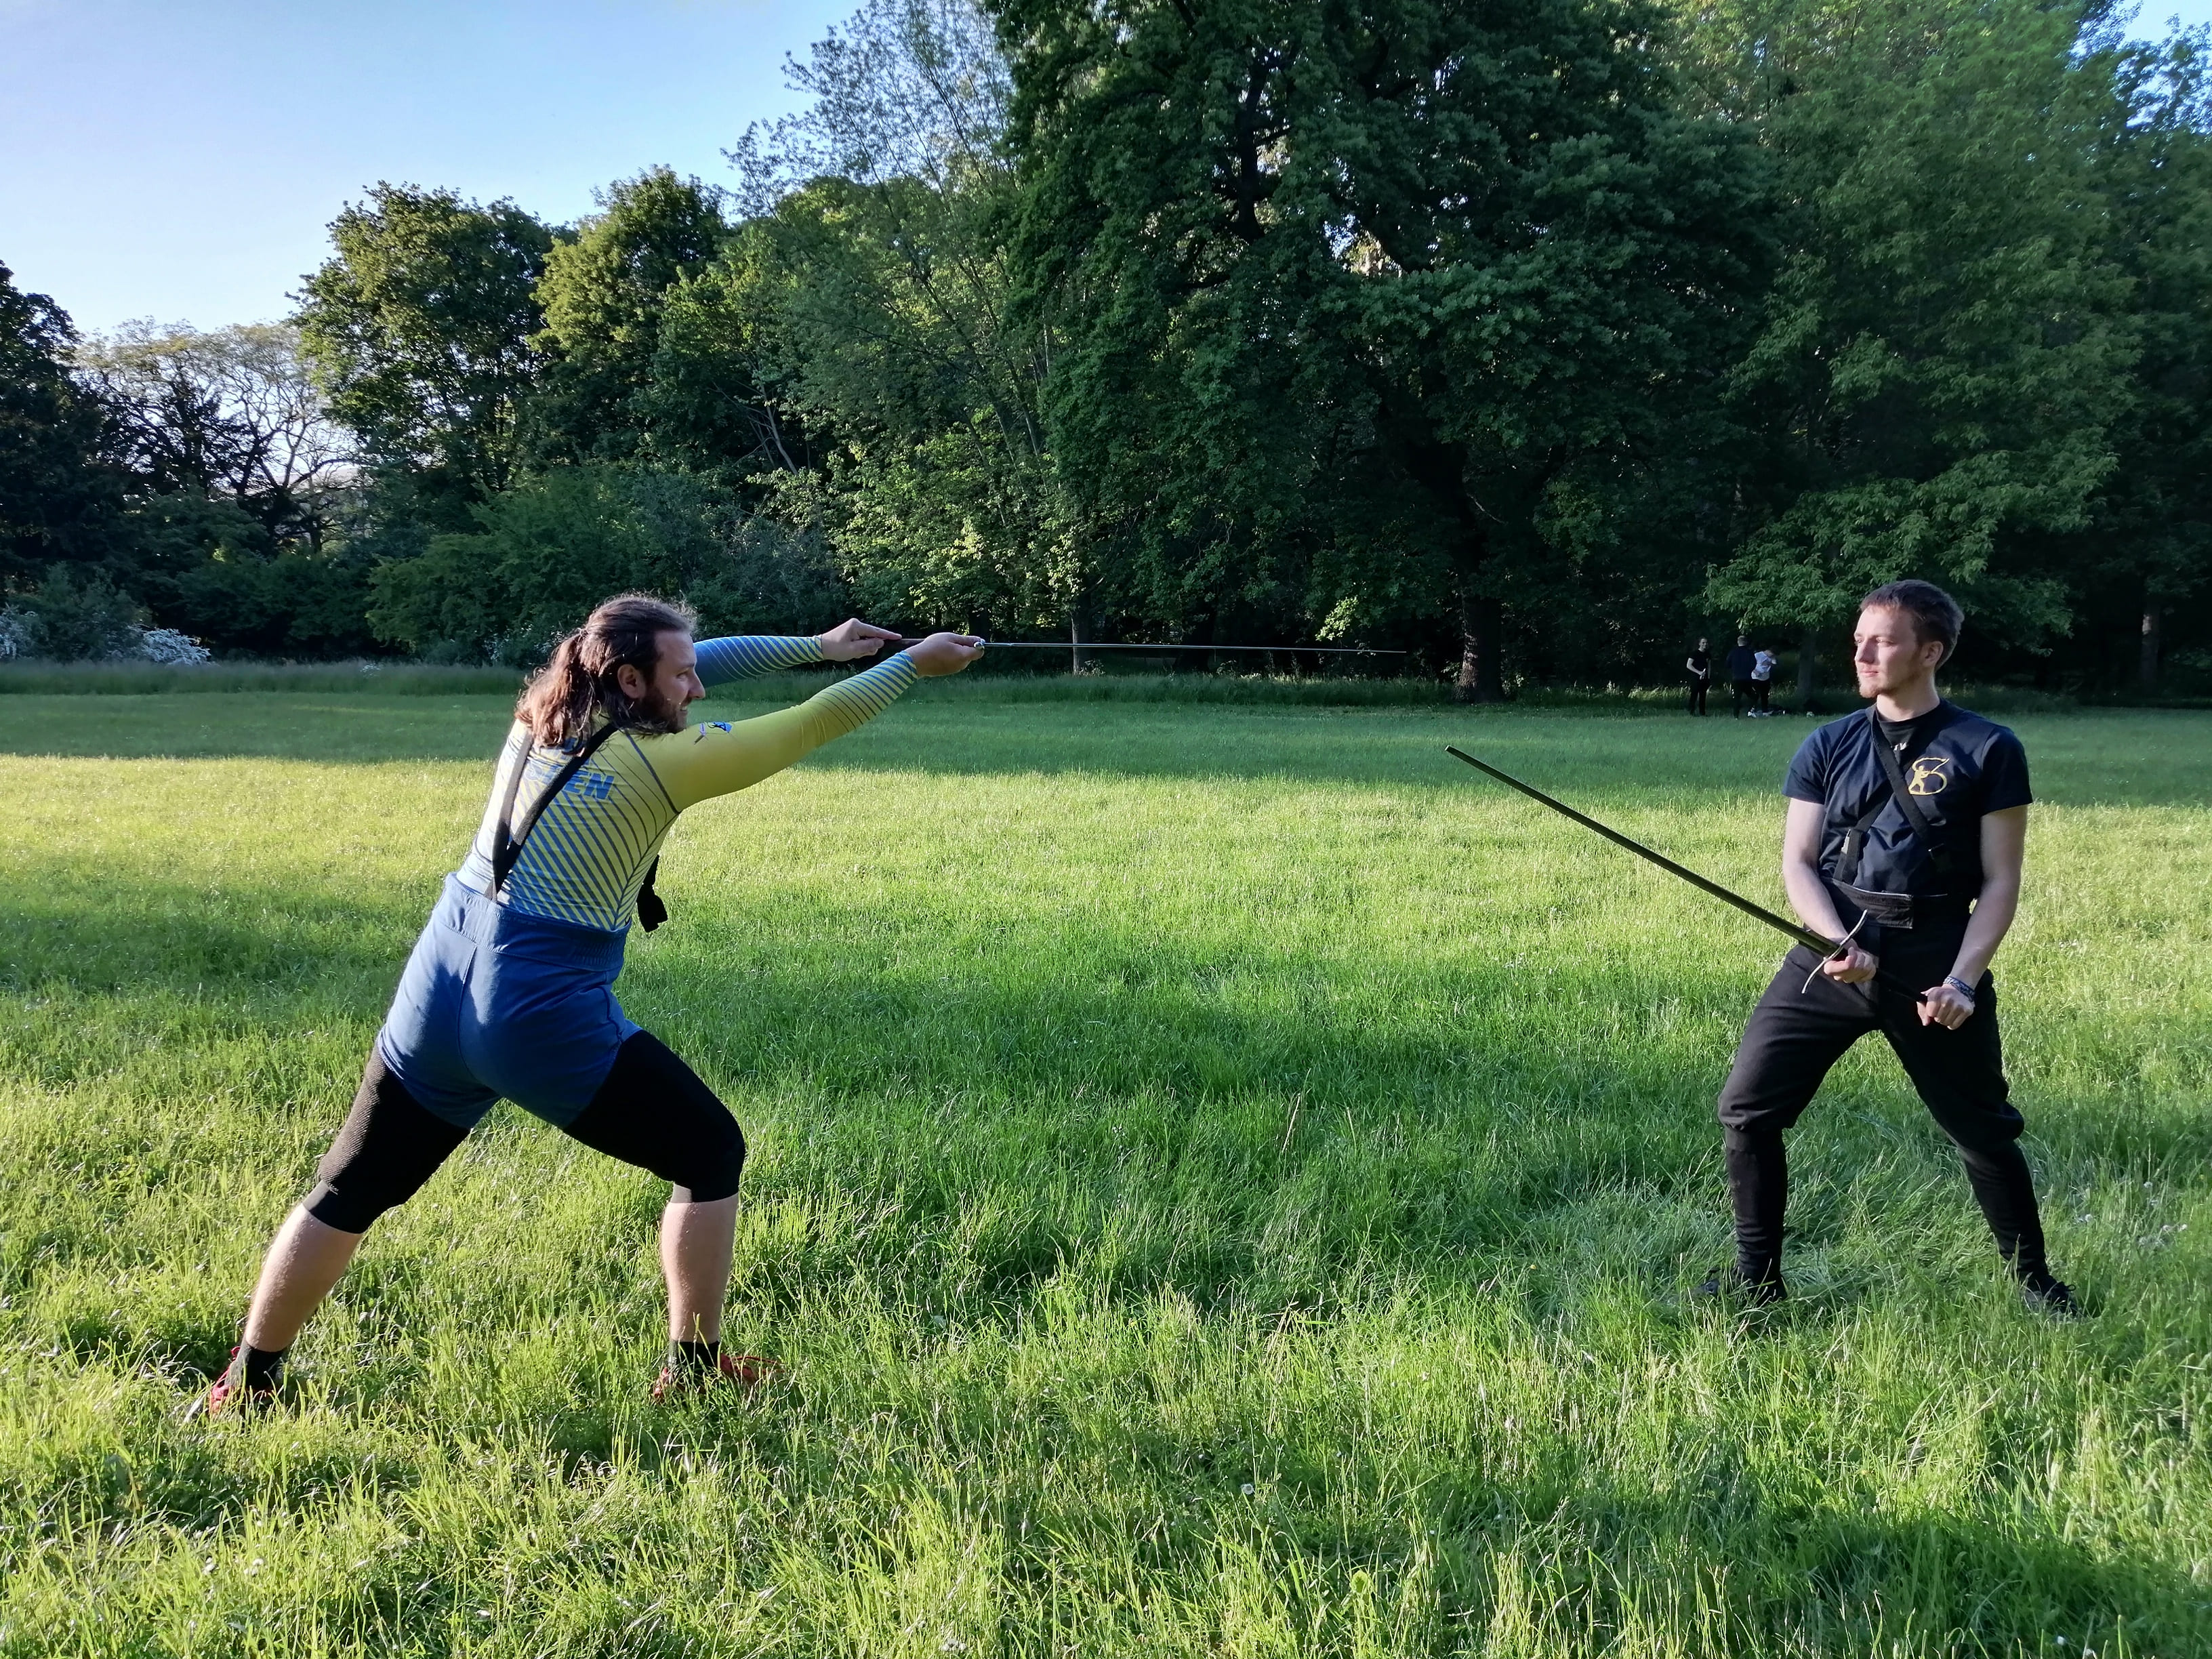
\includegraphics[scale=.075]{Weite2.jpg}
    \caption{Die Zufechtmensur}
    \label{fig:Zufechtmensur}
\end{figure}

Der:die Gegner:in kann mit der Klinge und nur einem Schritt erreicht werden.
\\
\FloatBarrier
\hrule
%\newpage

\paragraph{Kriegsmensur}

\FloatBarrier

\begin{figure}[!ht]
\minipage{0.45\textwidth}
  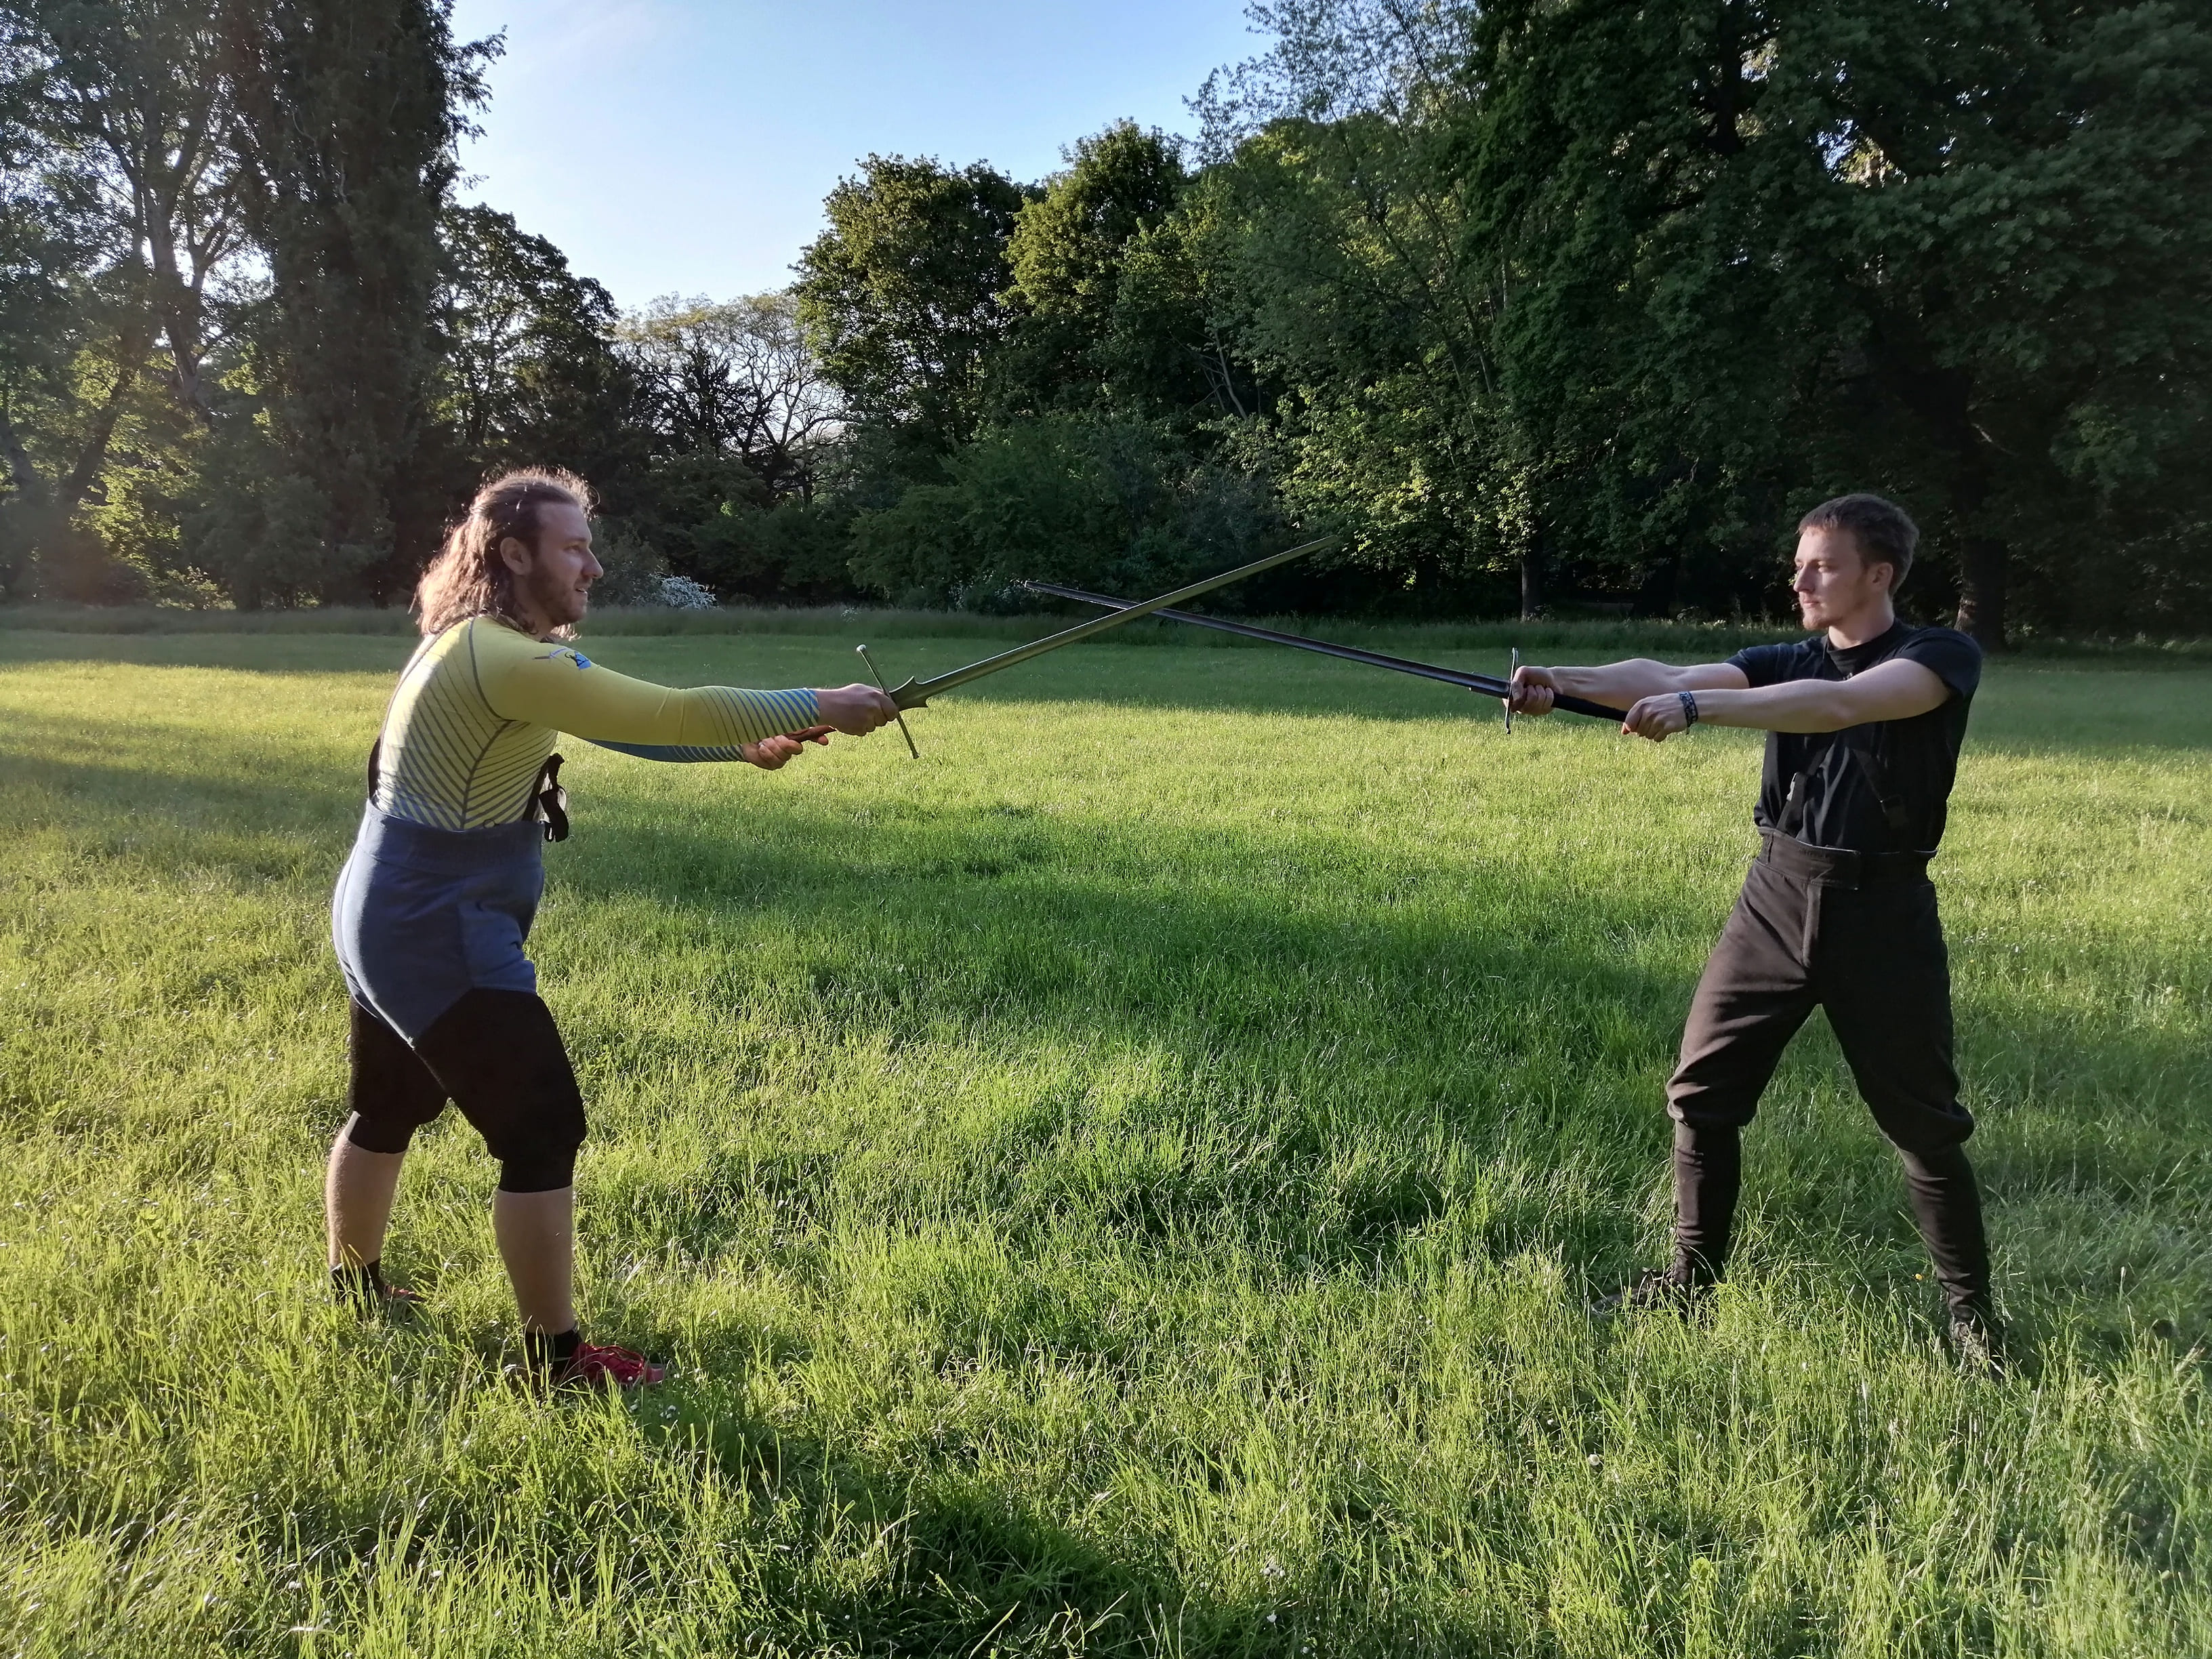
\includegraphics[width=\linewidth]{Langort.jpg}
  \caption{Eintritt in die Kriegsmensur}\label{fig:krieg1}
\endminipage\hfill
\minipage{0.45\textwidth}
  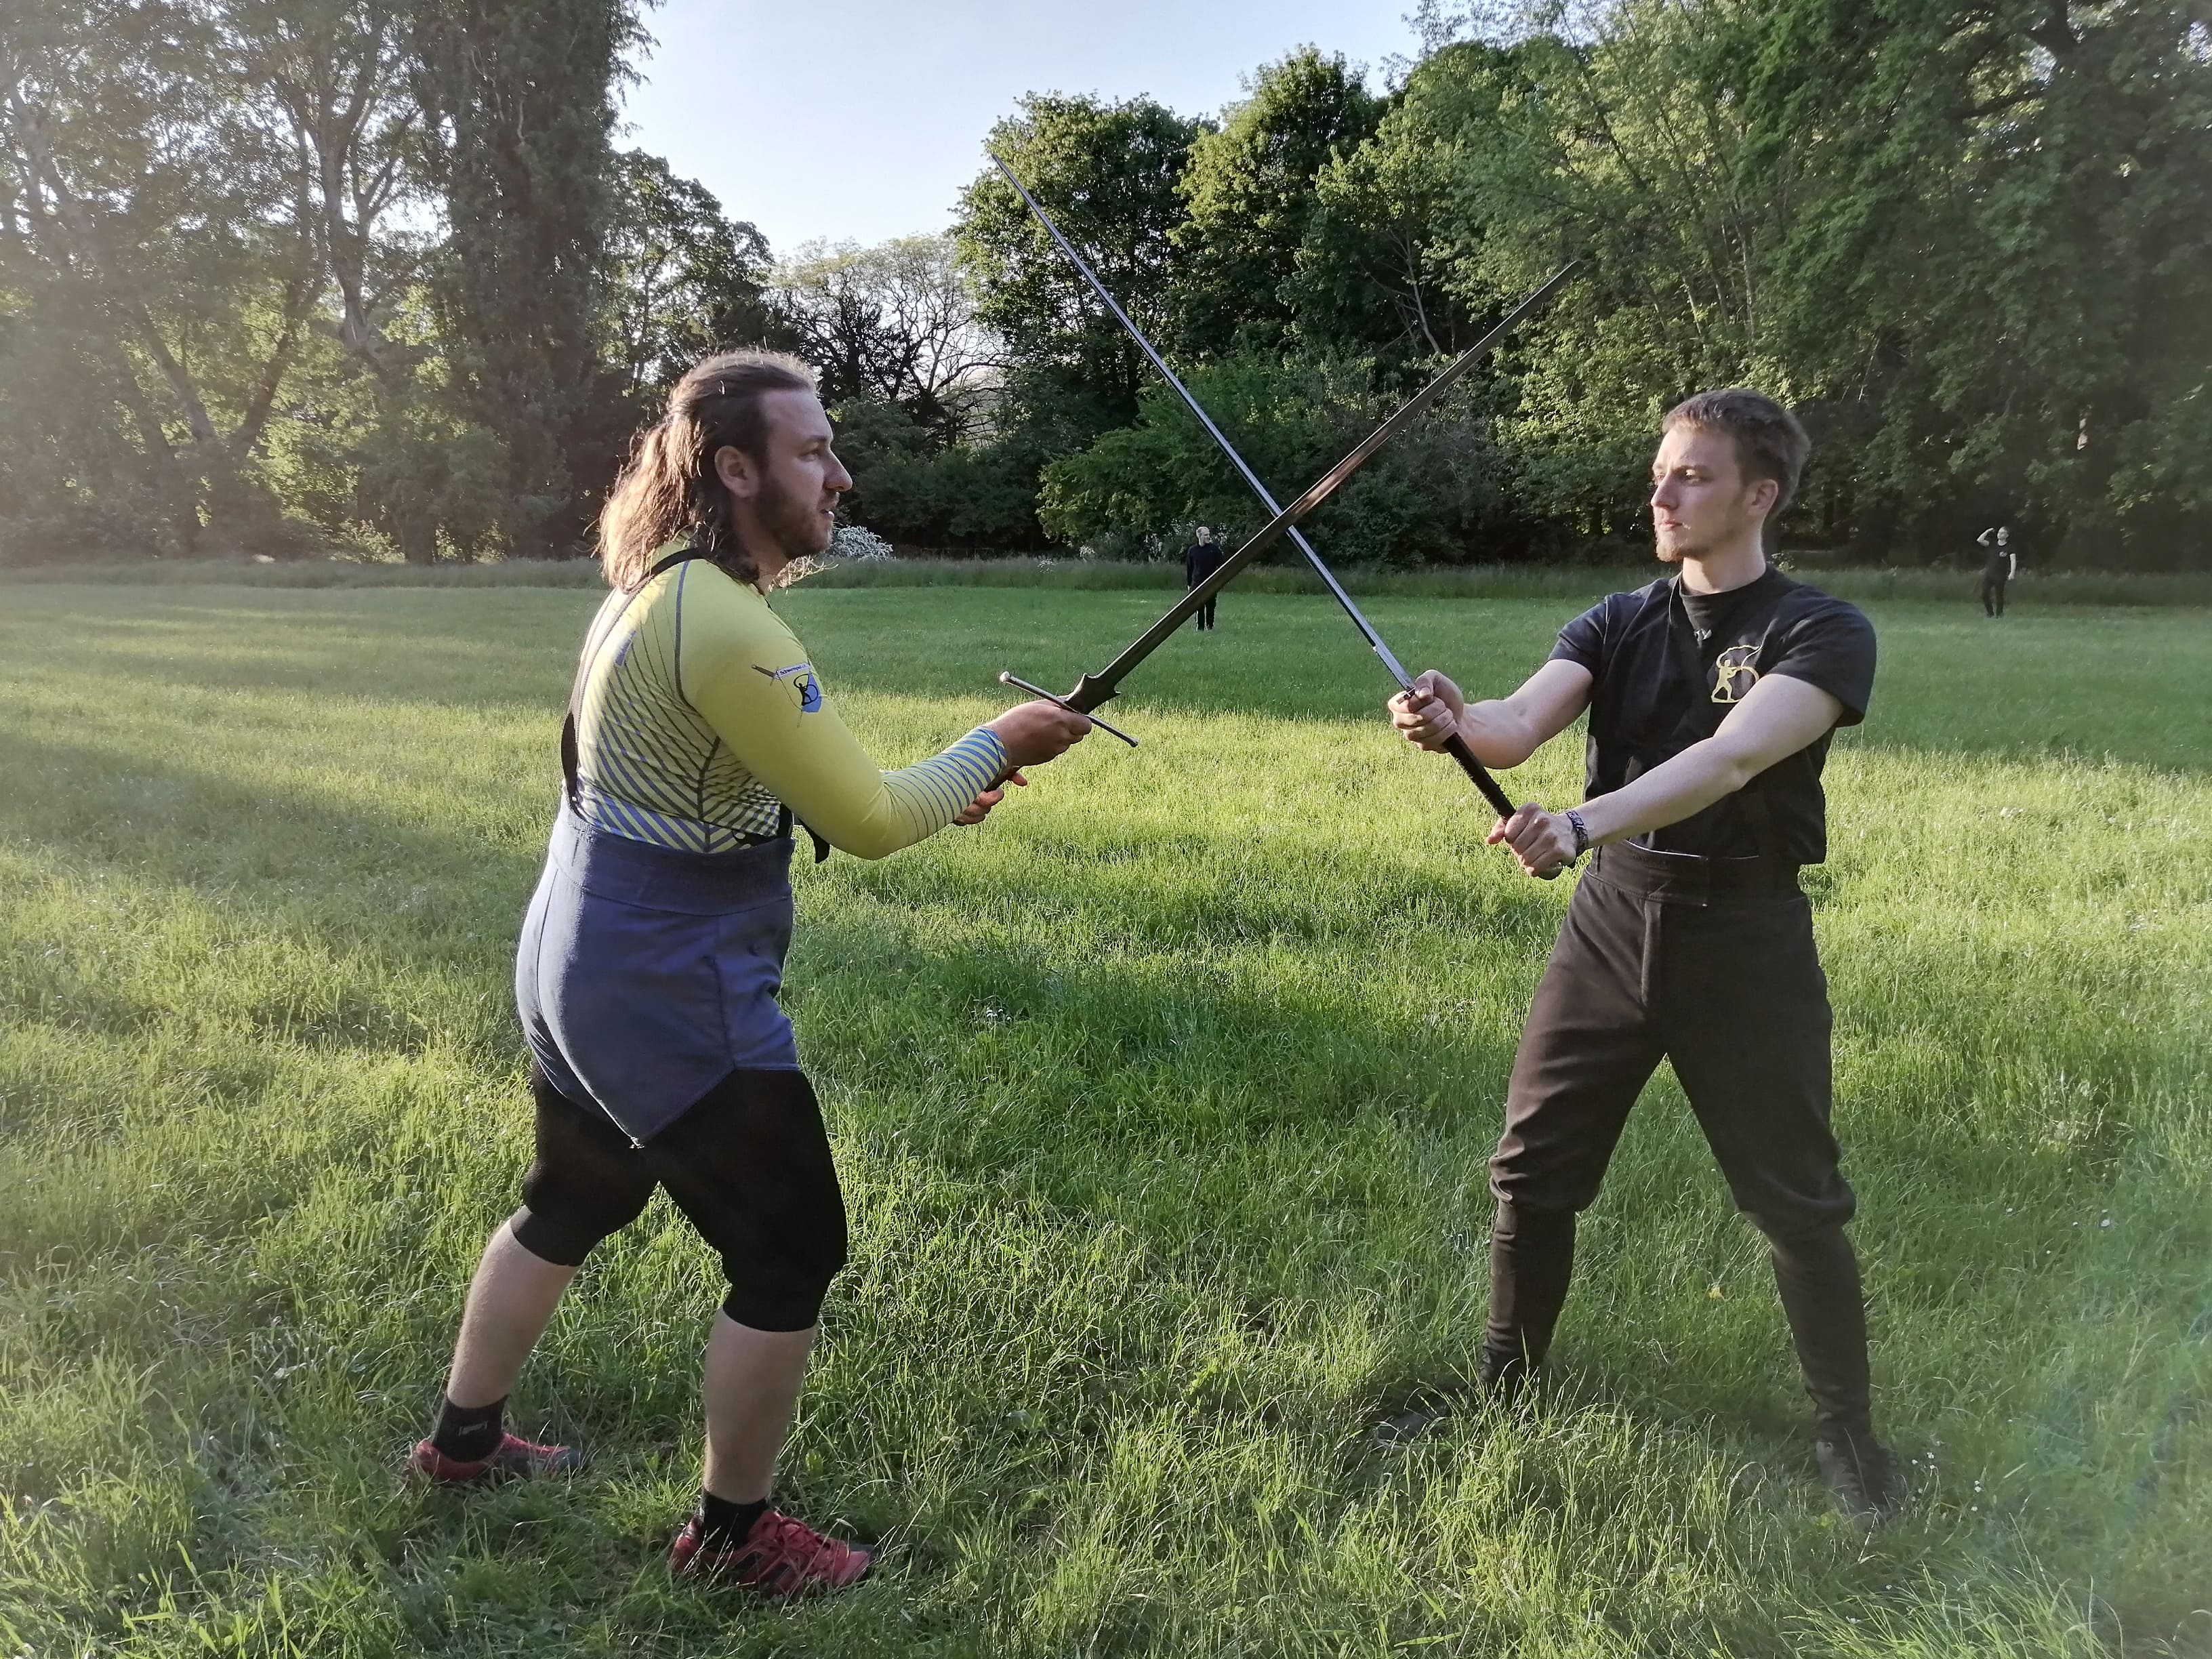
\includegraphics[width=\linewidth]{Schnitt1.jpg}
  \caption{Austritt aus der Kriegsmensur}\label{fig:krieg2}
\endminipage\hfill

\end{figure}

Das Gegenüber ist ohne Schritt erreichbar. Hier geschieht die Bindungsarbeit.

\FloatBarrier

\newpage

\paragraph{Ringmensur I: Das Armringen}

\begin{figure}[!ht]
    \centering
    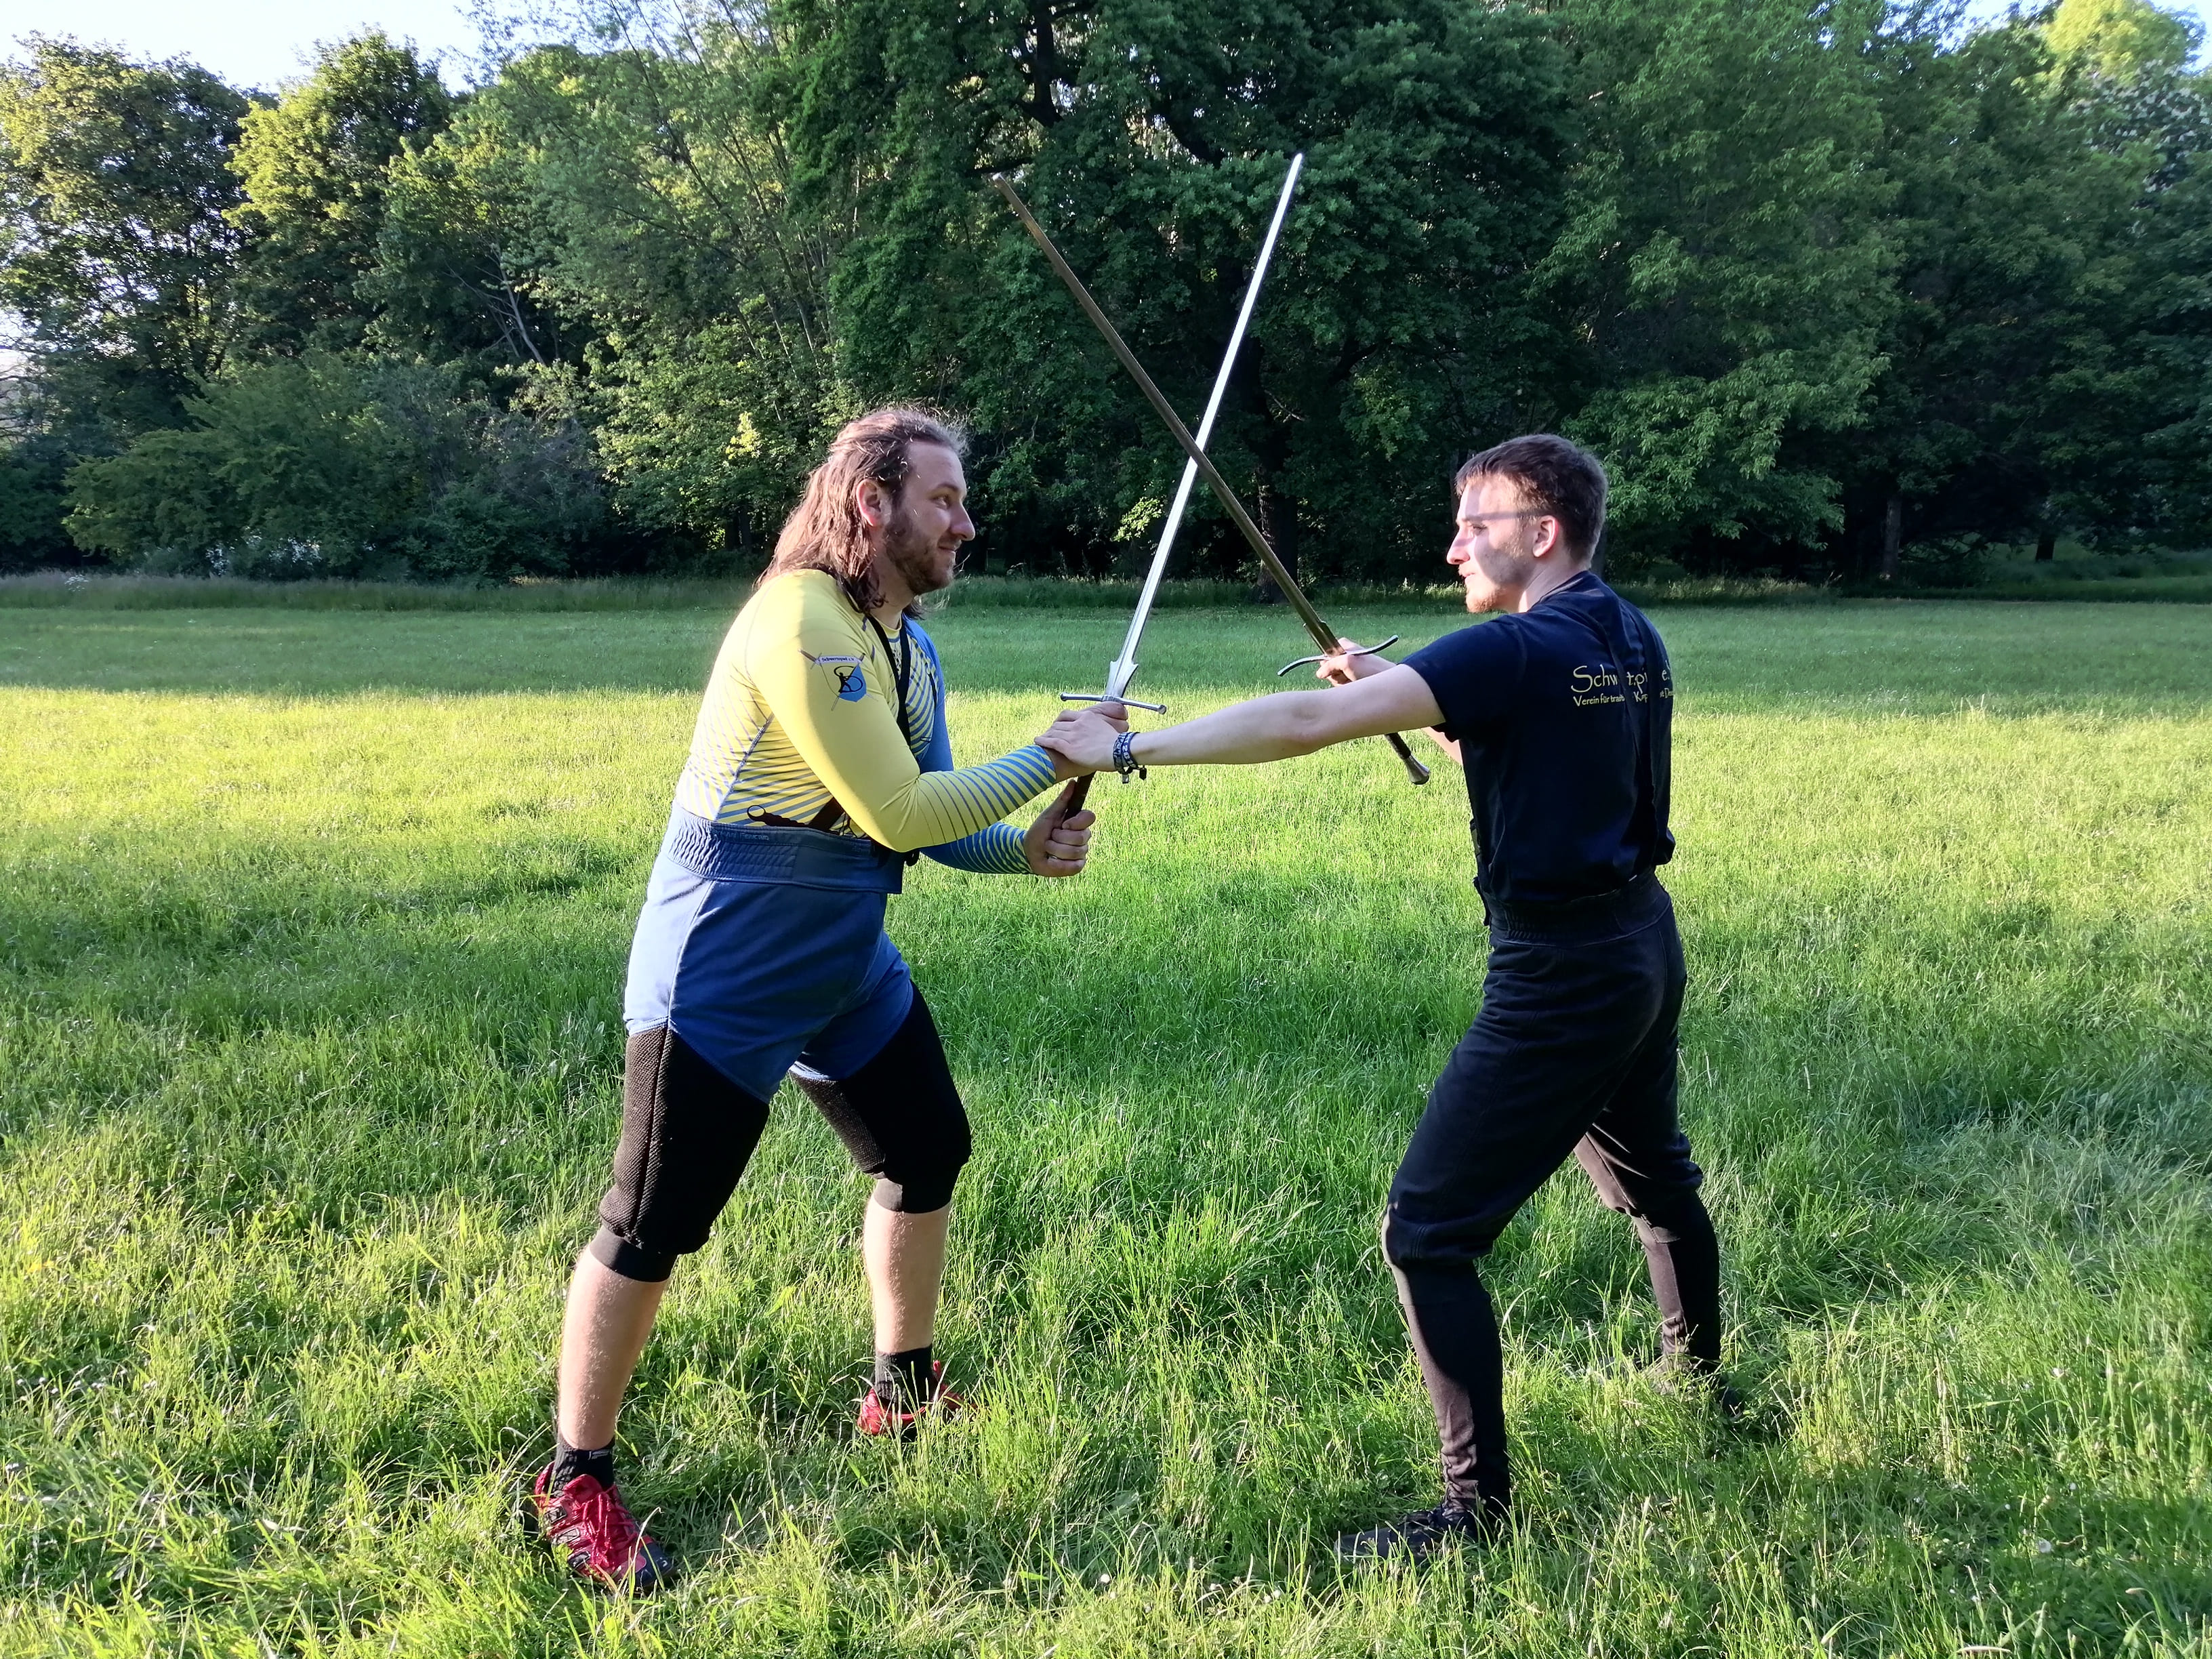
\includegraphics[scale=.075]{Eng1.jpg}
    \caption{Das Armringen}
    \label{fig:Armringen}
\end{figure}

Man erreicht mit der eignen Hand die Arme des Gegenübers. Armringen und Schwertnehmen sind möglich, weite Häue verlieren an Effekt.
\\
\hrule

\paragraph{Ringmensur II: Das Leibringen}

\begin{figure}[!ht]
    \centering
    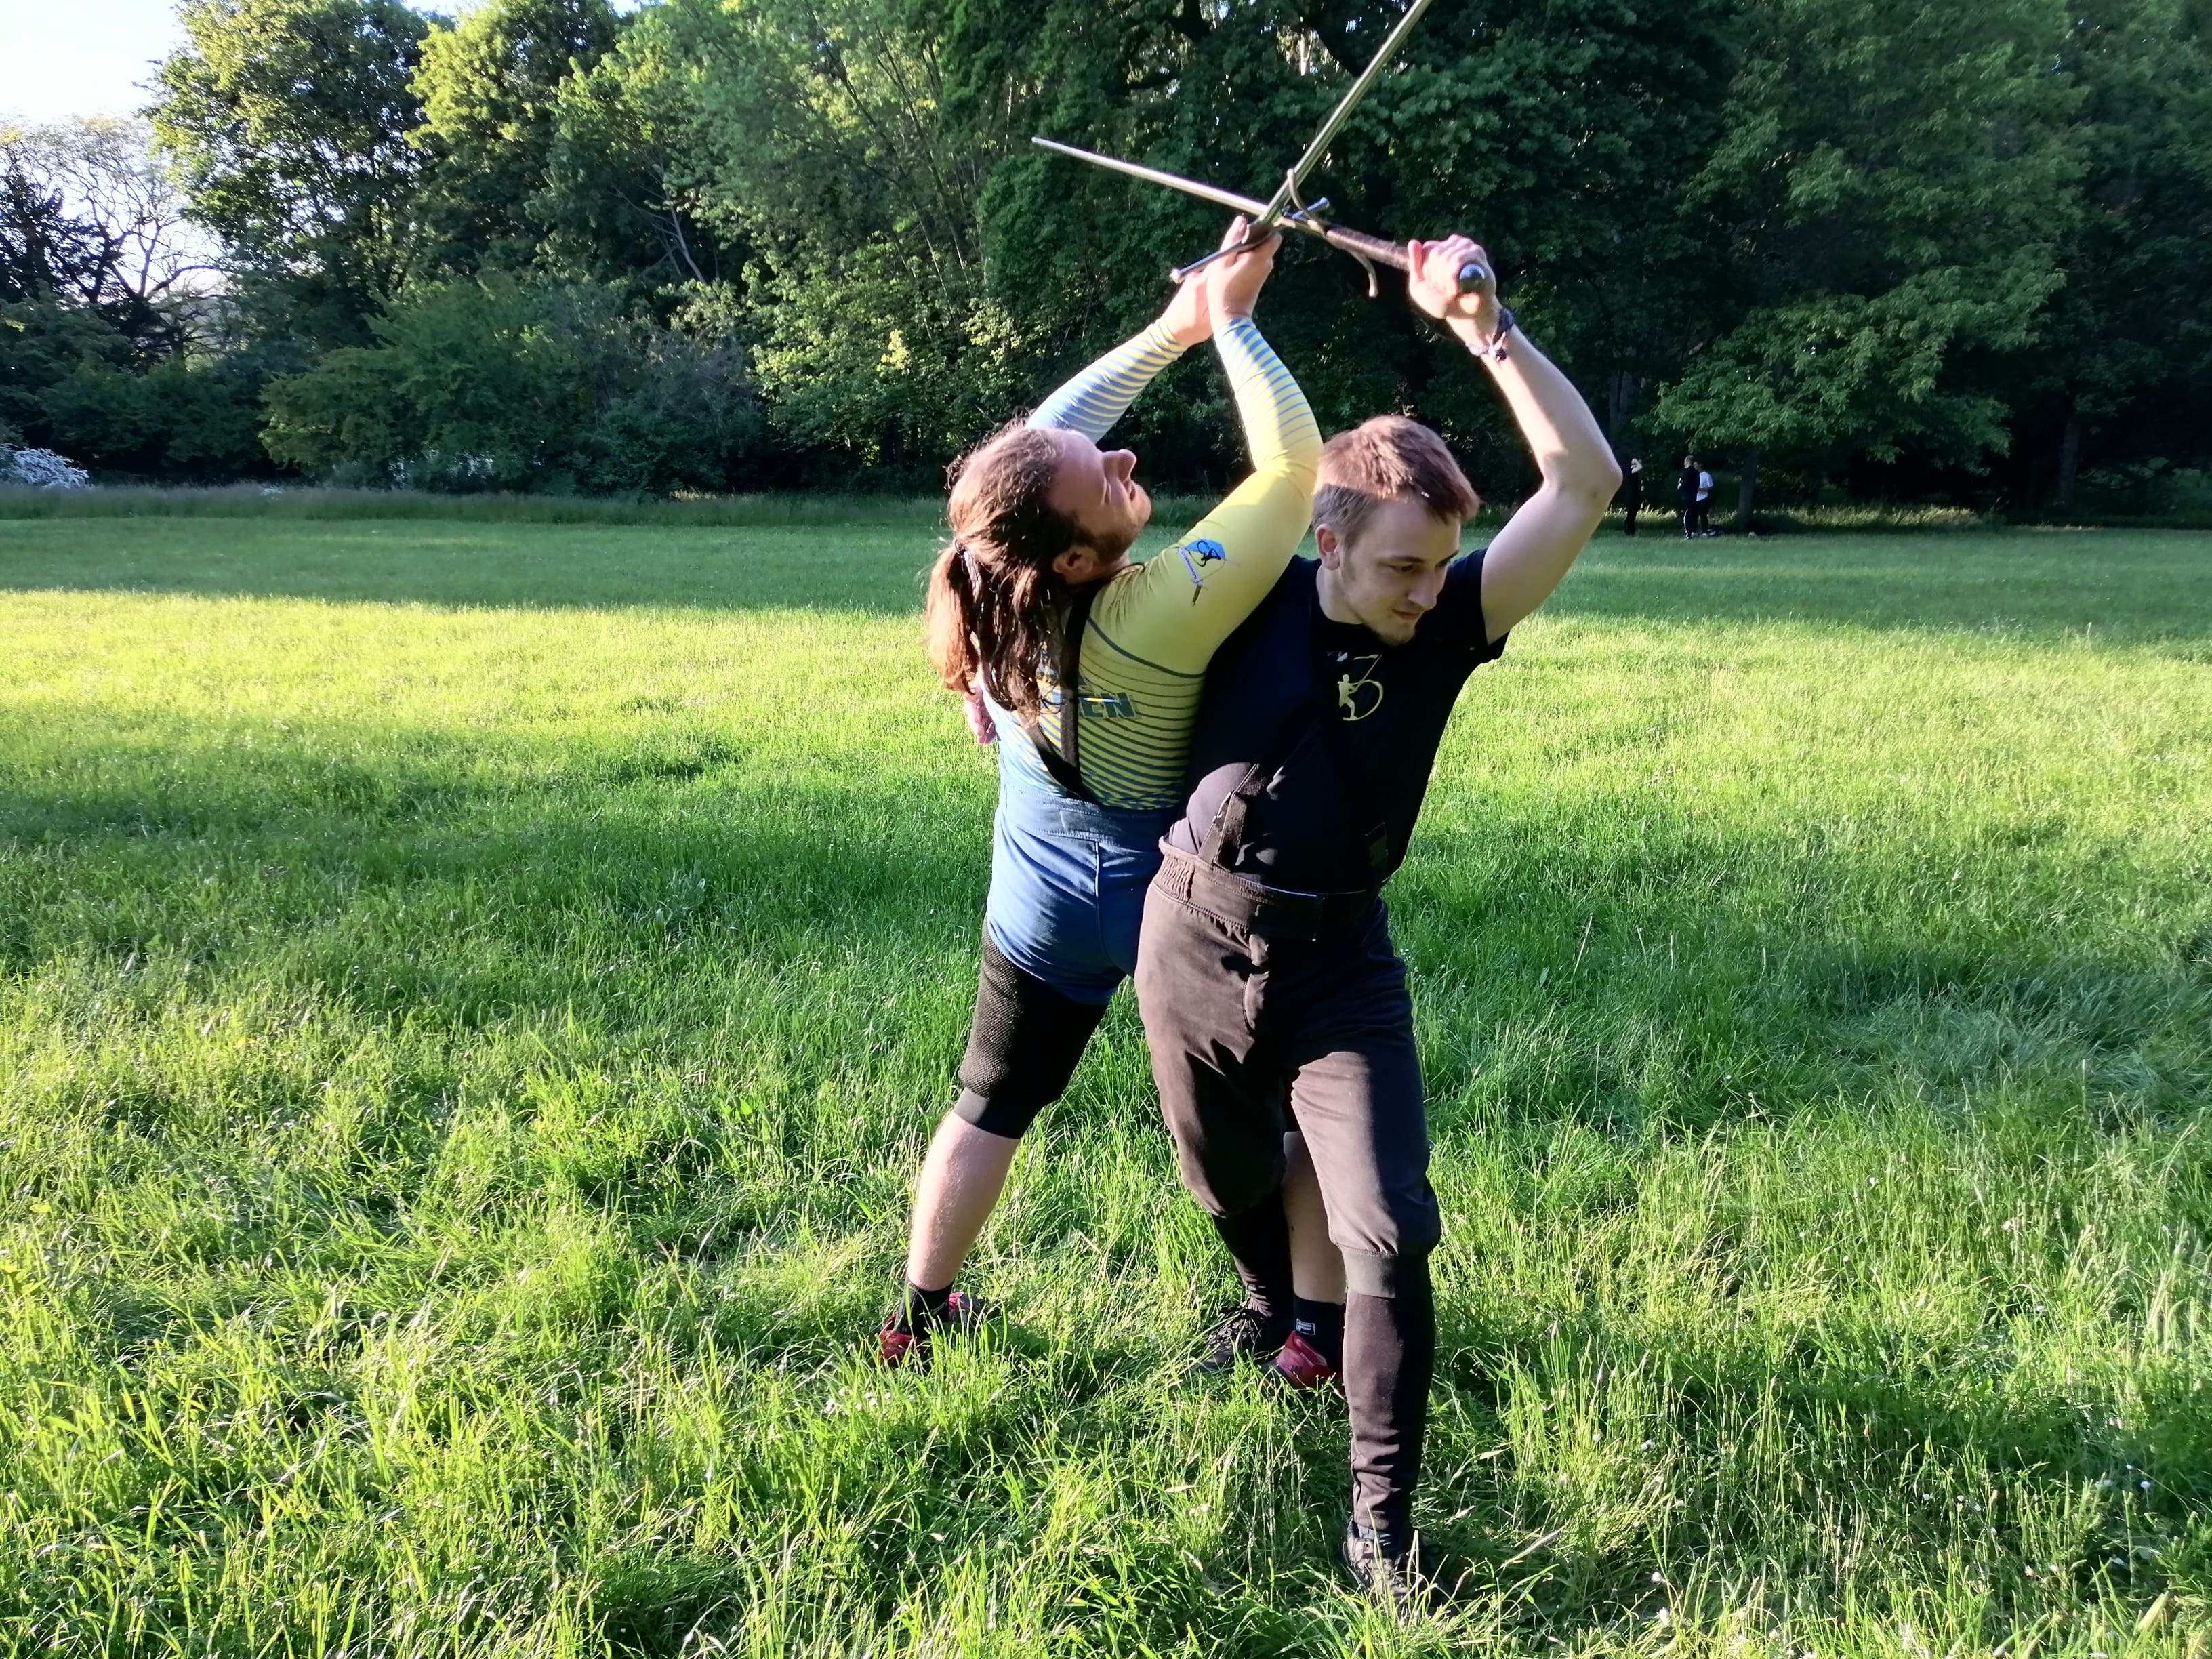
\includegraphics[scale=.075]{Ringe1.jpg}
    \caption{Das Leibringen}
    \label{fig:Leibringen}
\end{figure}

Der Körper des Gegenübers kann direkt angegriffen werden, Körperringstücke sind möglich.

\newpage

\subsubsection{Bindung}\label{Bindung0}

Die Bindung (oder das Band) beschreibt das Verhalten zweier sich berührender Klingen. Das Aufeinandertreffen der Klingen wird als Anbinden bezeichnet.
\\
\\
Lässt sich das Schwert des Gegenübers nach dem Aufeinandertreffen verdrücken, ist dies eine weiche oder schwache Bindung. Wird man hingegen selbst verdrückt oder kann das Schwert des Gegenübers selbst nicht bewegen, spricht man von einer harten oder starken Bindung.
\\
\\
Allgemein ist eine Bindung von oben über die Klinge des Gegners stärker. Eine Bindung mit Schneider auf Fläche hat in der Regel ebenfalls einen Vorteil.
\\
\\
Die Geometrie und das Kräfteverhältnis im Band werden zudem durch die Stelle der Anbindung bestimmt. Da scharfe Klingen in der Regel aneinenader haften (oder ''beißen''), erhält sich dieses Klingenverhältnis bis es aktiv aufgelöst oder geändert wird.
\\
\\
Liegt man mit der eigenen Schwäche in der Stärke des:der Gegner:in, hat diese:r einen starken Karftvorteil. Gleiches gilt auch umgekehrt.
\\
\\
Von einer ''neutralen Bindung'' wird gesprochen, wenn beide Klingen mittig und ohne erkennbaren geometrischen Vorteil anbinden.

\subsubsection{Vor, Nach und Indes}

Der Begriff ''Tempo'' beschreibt im historischen Fechten das zeitliche Verhältnis zweier Fechter:innen oder dient als ''zeitliche Einheit'' für fechterische Aktionen.
\\
\\
Besitzt man die Initiative und zwingt so den:die Gegner:in zum versetzen, so ficht man aus dem ''Vor''. Behält man das ''Vor'', so gibt man dem:der Gegner:in keine Möglichkeit, selbst Aktionen zu beginnen, so lange diese:r auf Eigenschutz achtet.
\\
\\
Muss man jedoch selbst auf einen Angriff reagieren, und ficht aus der Versatzung schnell zur nächsten Blöße, so bricht man das ''Vor'' des:der Gegner:in mit dem eigenen ''Nach''.
\\
\\
Das ''Indes'' liegt zwischen ''Vor'' und ''Nach''. Es beschreibt eine Aktion, die während der eines:einer Gegner:in ausgeführt wird.
\\
\\
Grundsätzlich ist es immer vorteilhaft, sich im ''Vor'' zu befinden, das heißt im Kampf die Initiative zu besitzen. Auf ein gegnerisches "Vor" wird im Idealfall mit einem eigenen "Indes" geantwortet, um dieses zu brechen.

\subsection{Fechterische Grundprinzipien} 

Alle von den Fechtmeistern beschriebenen Stücke folgen grundlegenden Prinzipien. Diese sind zwar meist nicht explizit beschrieben und doch ziehen sich ähnliche Muster, Annahmen und Regeln wie ein roter Faden über die Autoren und Bücher hinweg durch alle Quellen. Nachfolgend wurden deshalb einige Grundlegende Prinzipien zusammengetragen, welche alle Fechtenden für das Interpretieren neuer Stücke verinnerlichen und anwenden sollten. Häufig können diese Prinzipien auch als Ziele eines Fechtstücks begriffen werden. Sollen mehrere Ziele gleichzeitig erfüllt werden kann es natürlich vorkommen, dass ein Interessenkonfilkt bei der Erfüllung der Ziele entsteht. In diesem Falle sollte die Interpretation den bestmöglichen Kompromiss für die Erfüllung aller Ziele bieten.

\subsubsection{Eigenschutz}

Die meisten Quellen mit Bezug zum Langen Schwert oder zum Langen Messer befassen sich mit dem sogenannten „Blossfechten“ also dem Fechten ohne jegliche Schutzausrüstung. In diesem Kontext wird ein Treffer sehr wahrscheinlich fatale Konsequenzen für den Getroffen haben. Aus diesem Grund hat der Eigenschutz  immer höchste Priorität.
\\
\\
Eigenschutz kann durch mehrere Wege erreicht werden:

\begin{enumerate}[I.]
    \item Bewegung der eigenen Waffe zur Gefahrenquelle
    \item Bewegung der Füße/Beine um sich aus dem Gefahrenbereich (häufig der Schnittlinie eines Schwertes) zu bewegen, bspw. durch Austreten zur Seite
    \item Bewegung des Körpers um sich aus dem Gefahrenbereich zu bewegen, bspw. durch Verlagern des Oberkörpers hinter die Bewegungslinie des eigenen Schwertes
    \item Bewegung der gegnerische Waffe vom eigenen Körper weg; Dies kann durch eigene Motivation oder aber durch den:die Gegner:in selbst geschehen, bspw. wenn diese:r sich verschätzt
\end{enumerate}

\newpage

\subsubsection{Häue, Schnitte, Stiche - Die drei Wunder}

\paragraph{Häue}

Häue sind die klassischste und für viele die intuitivste Angriffsform mit dem langen Schwert. Ein effektiver Hau kann auch mit wenig Kraft geschlagen werden, sollte aber ausreichend Weg zur Beschleunigung ($\sim$30cm) haben, bevor er sein Ziel trifft. Ein Hau kann automatisch Selbstschutz herstellen, wenn er in die gedeckte Bindung geschlagen wird.
\\
\\
Oberhau:

\FloatBarrier

\begin{figure}[!htb]
\minipage{0.24\textwidth}
    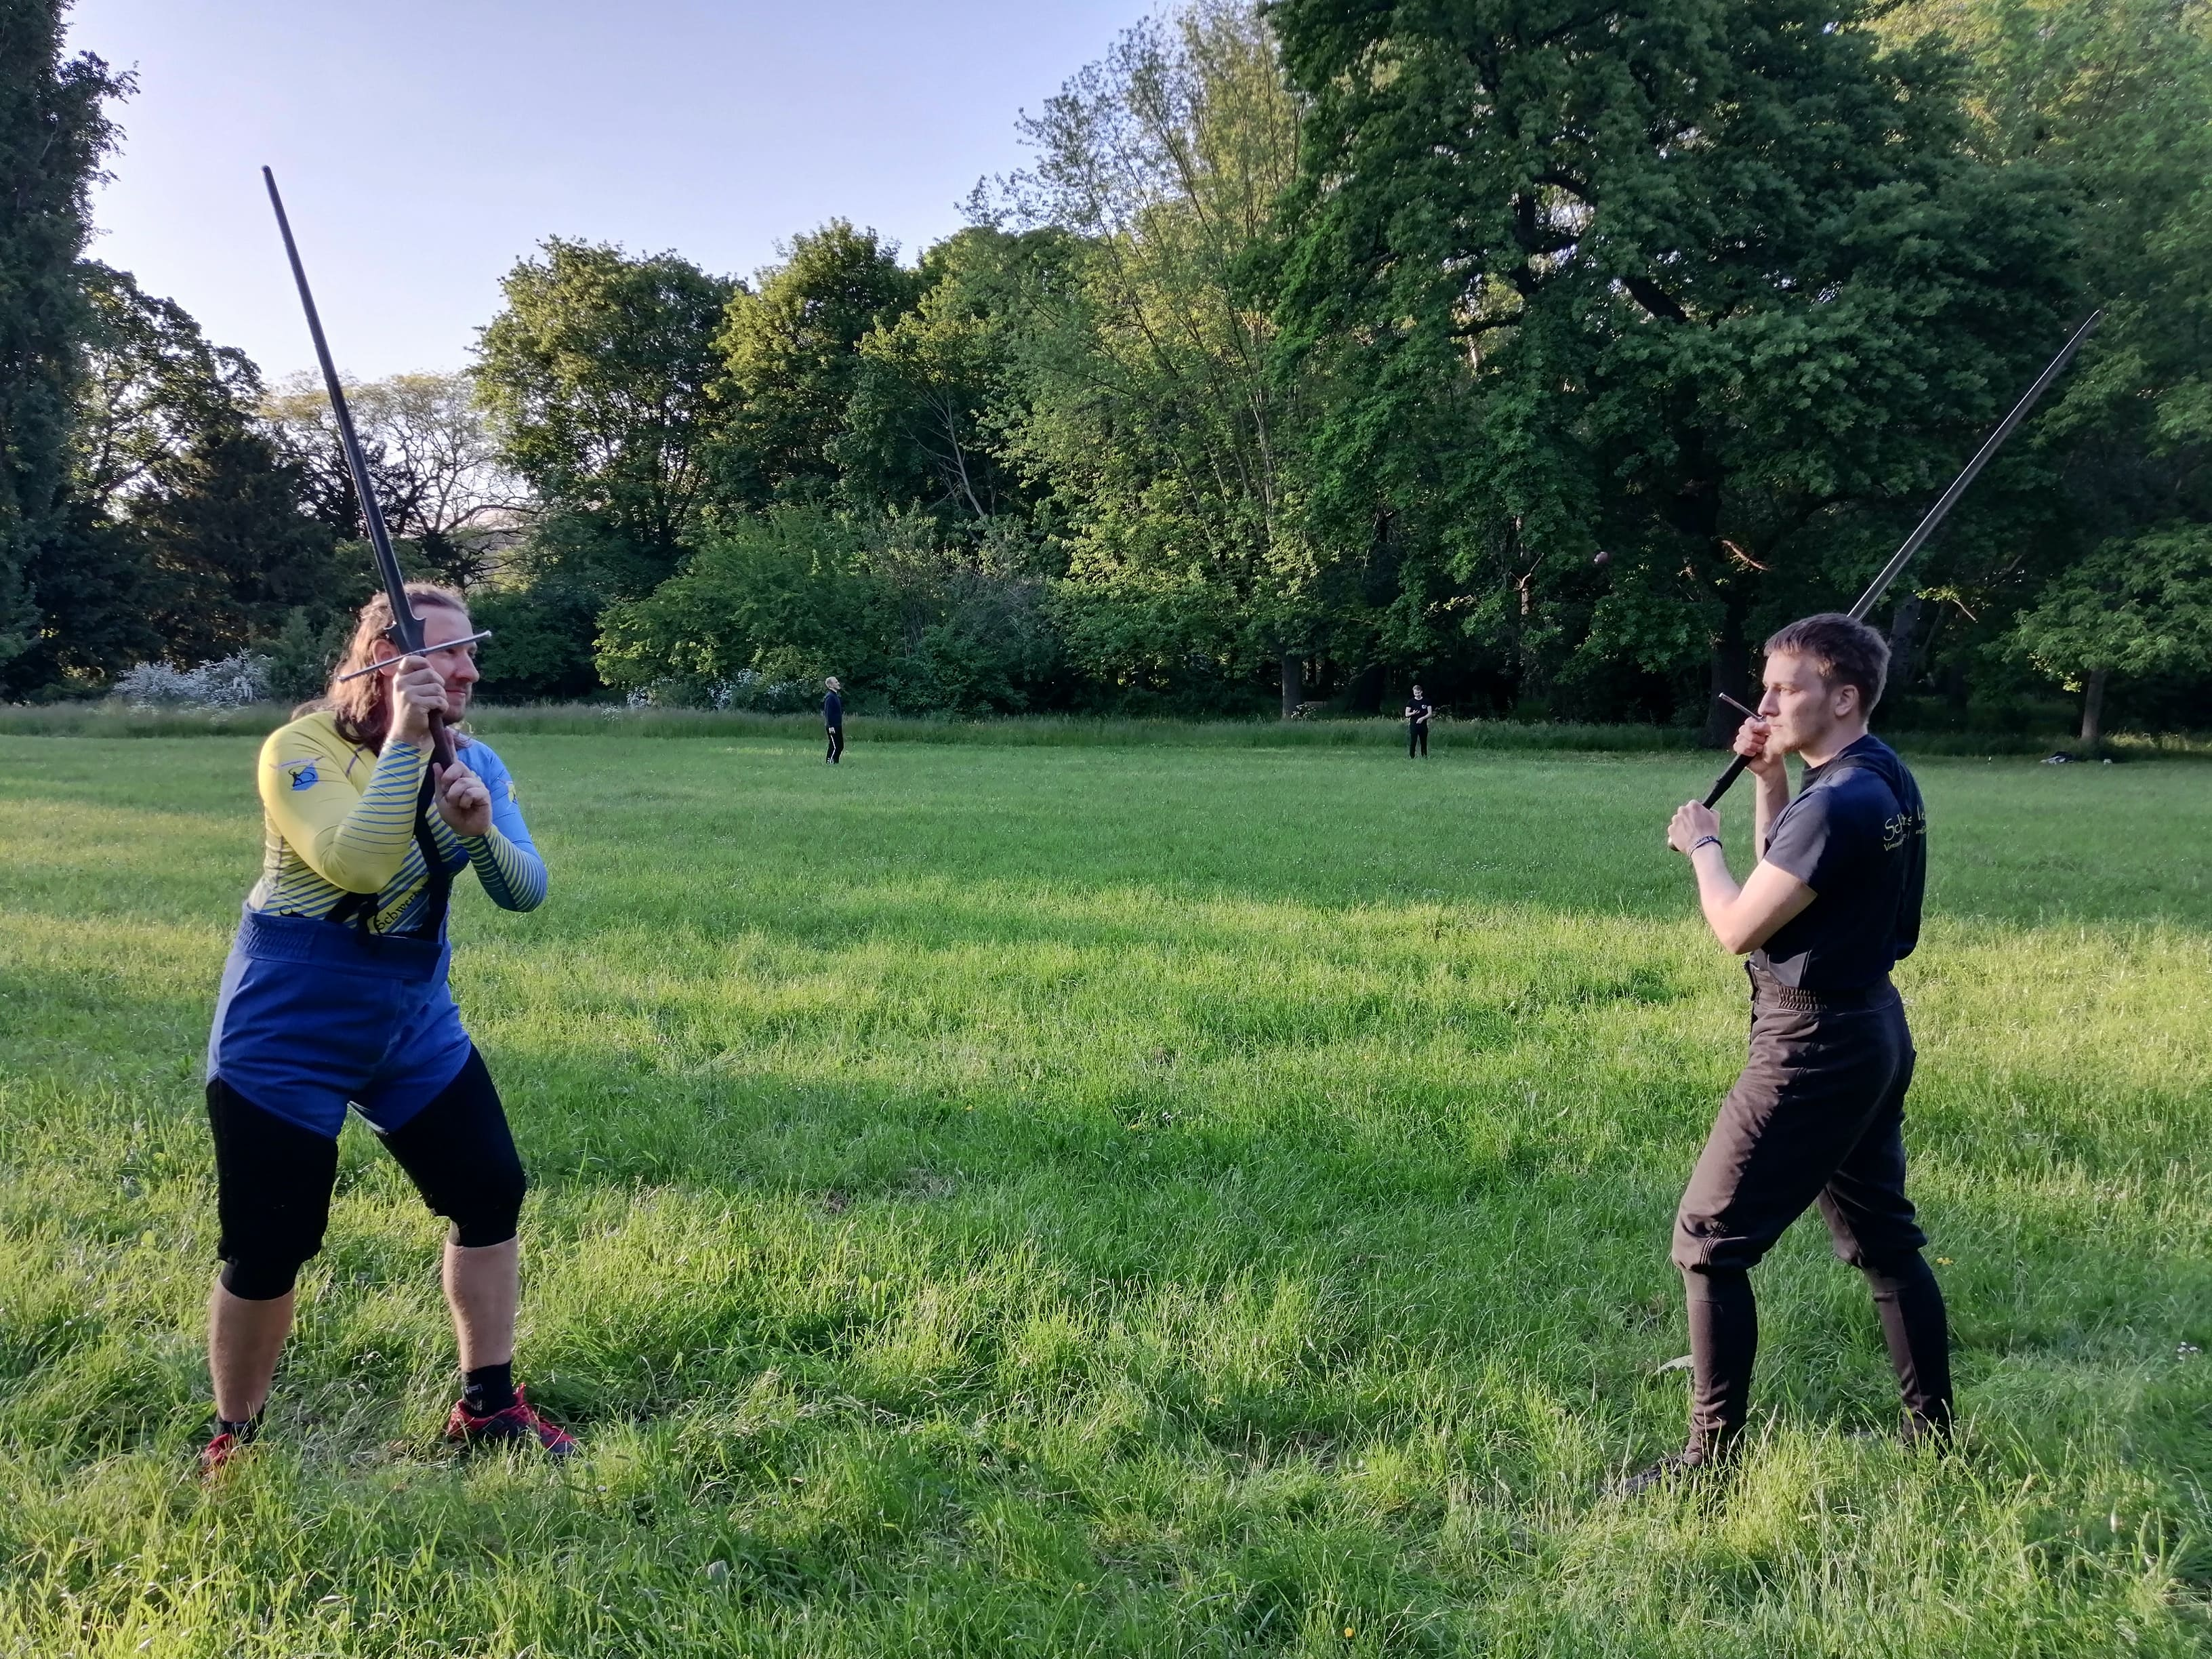
\includegraphics[width=\linewidth]{Oberhau1.jpg}
\endminipage\hfill
\minipage{0.24\textwidth}
    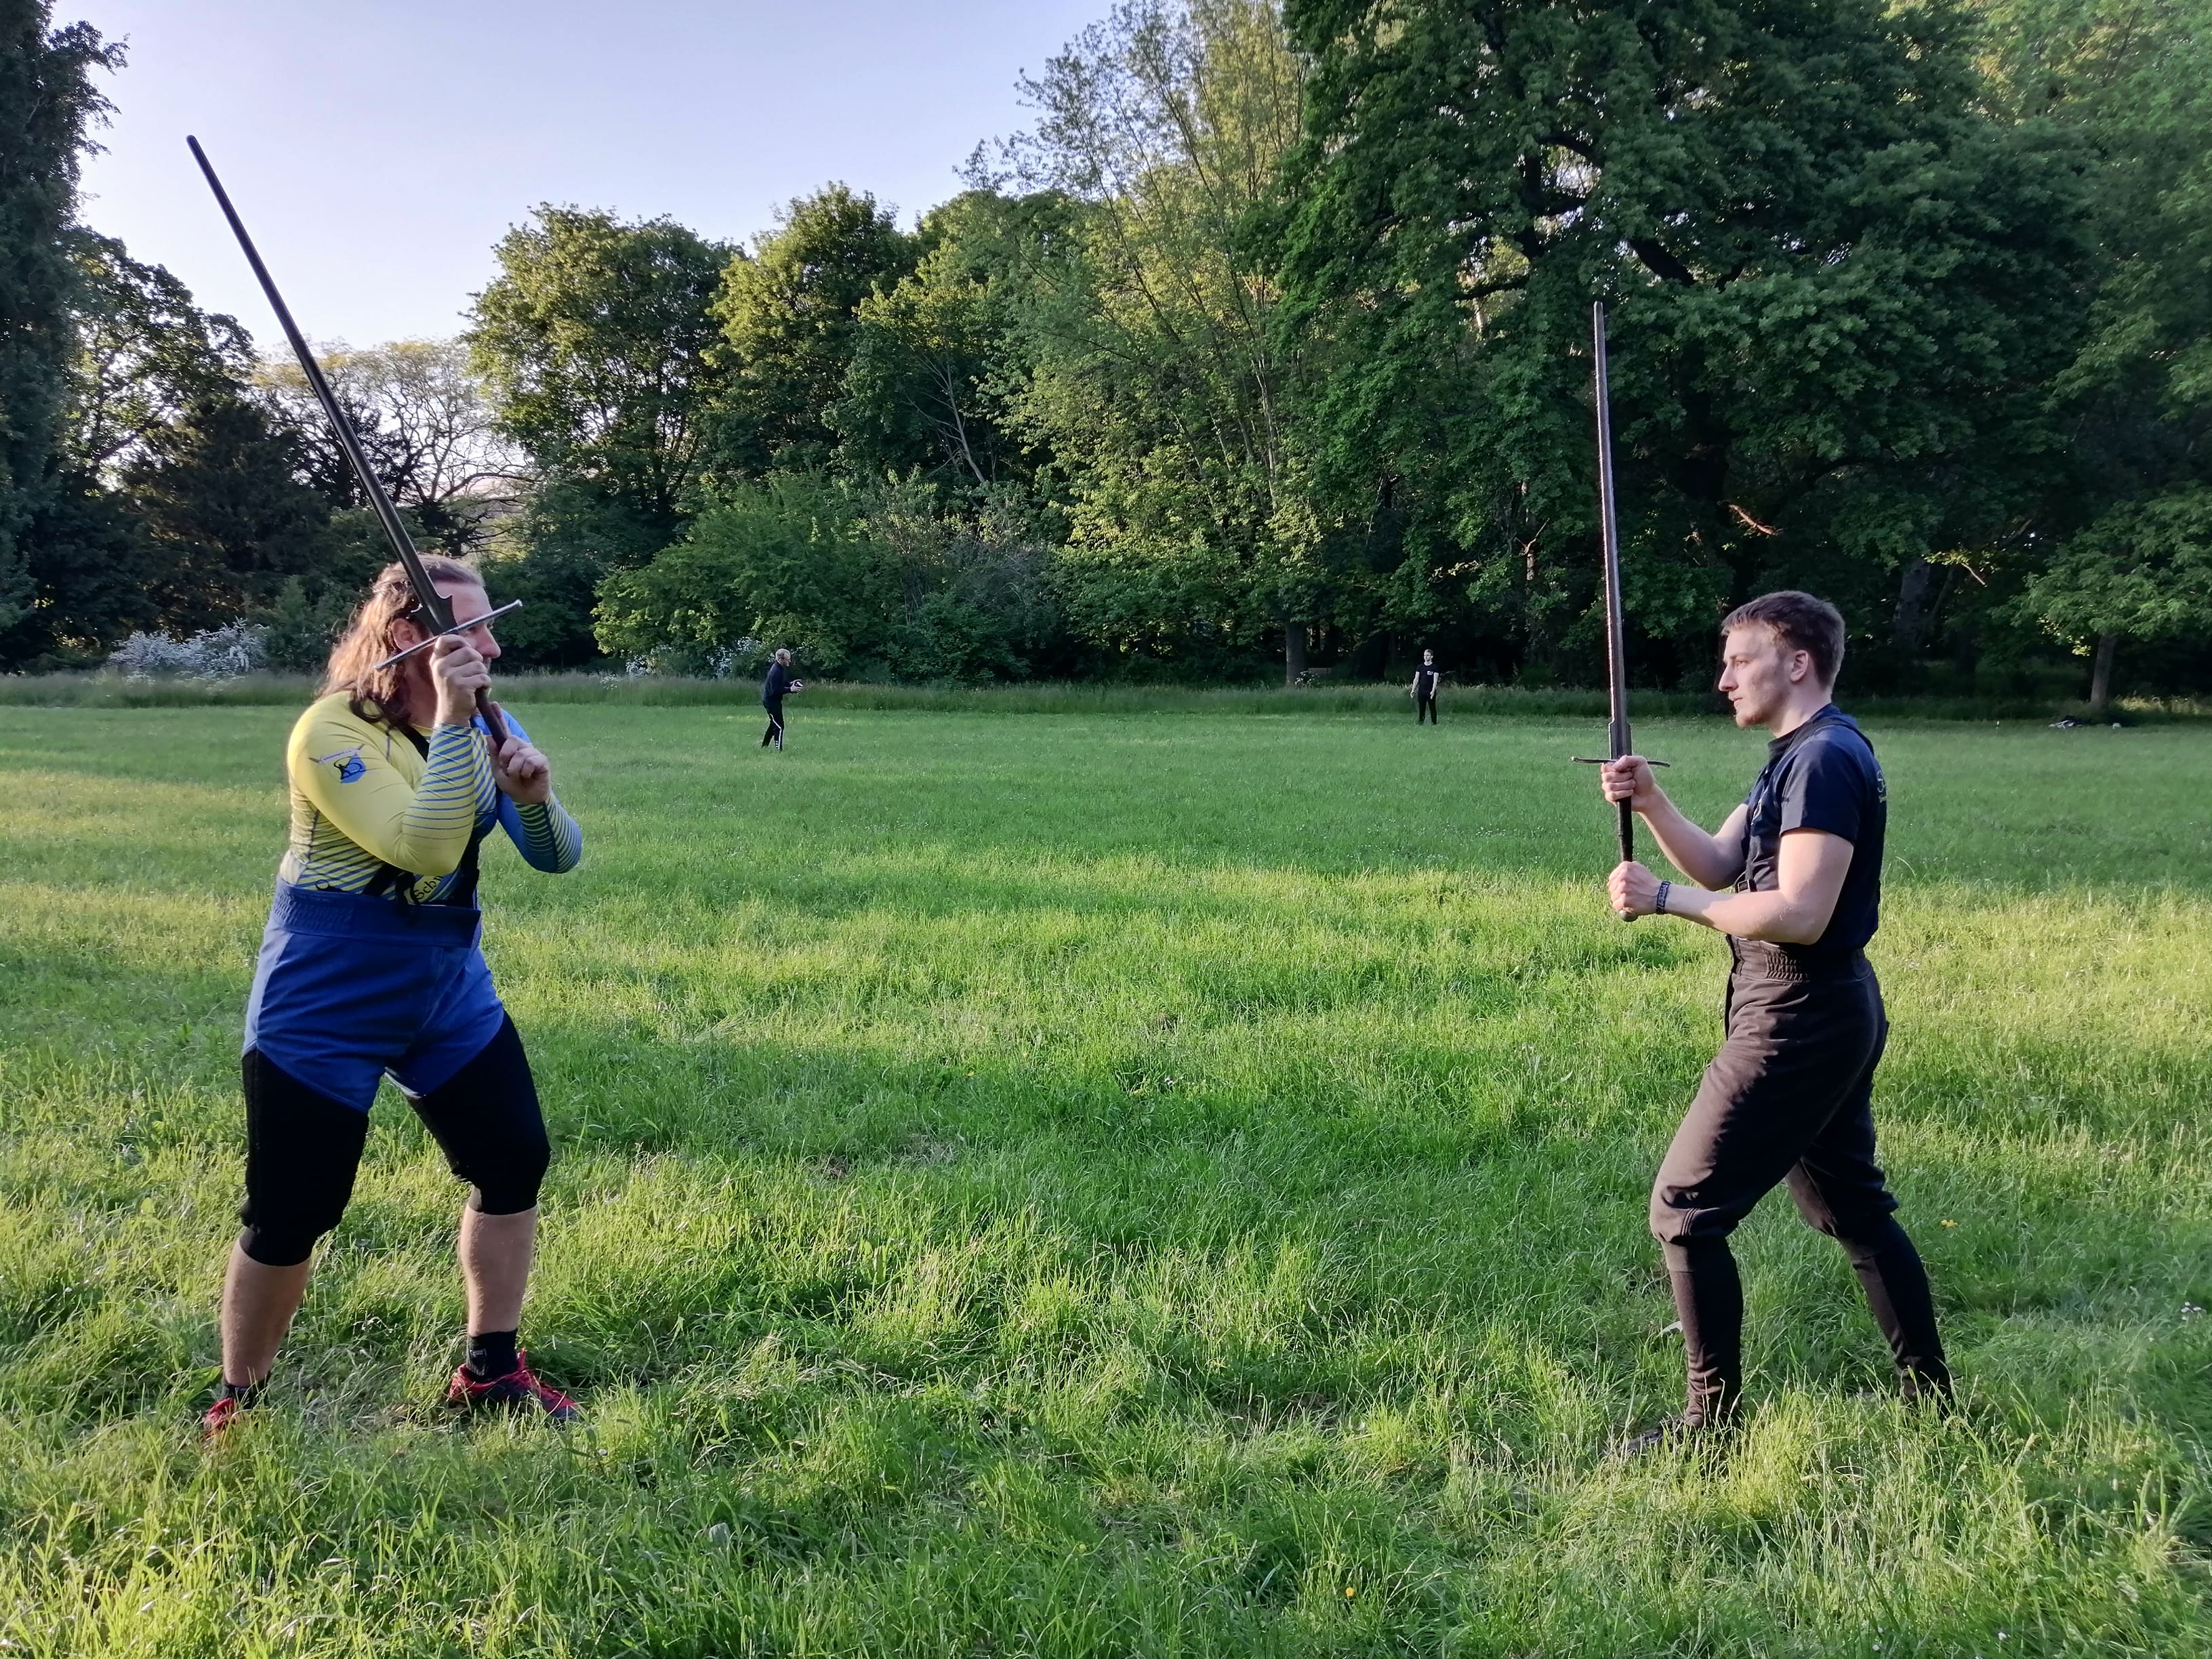
\includegraphics[width=\linewidth]{Oberhau2.jpg}
\endminipage\hfill
\minipage{0.24\textwidth}
    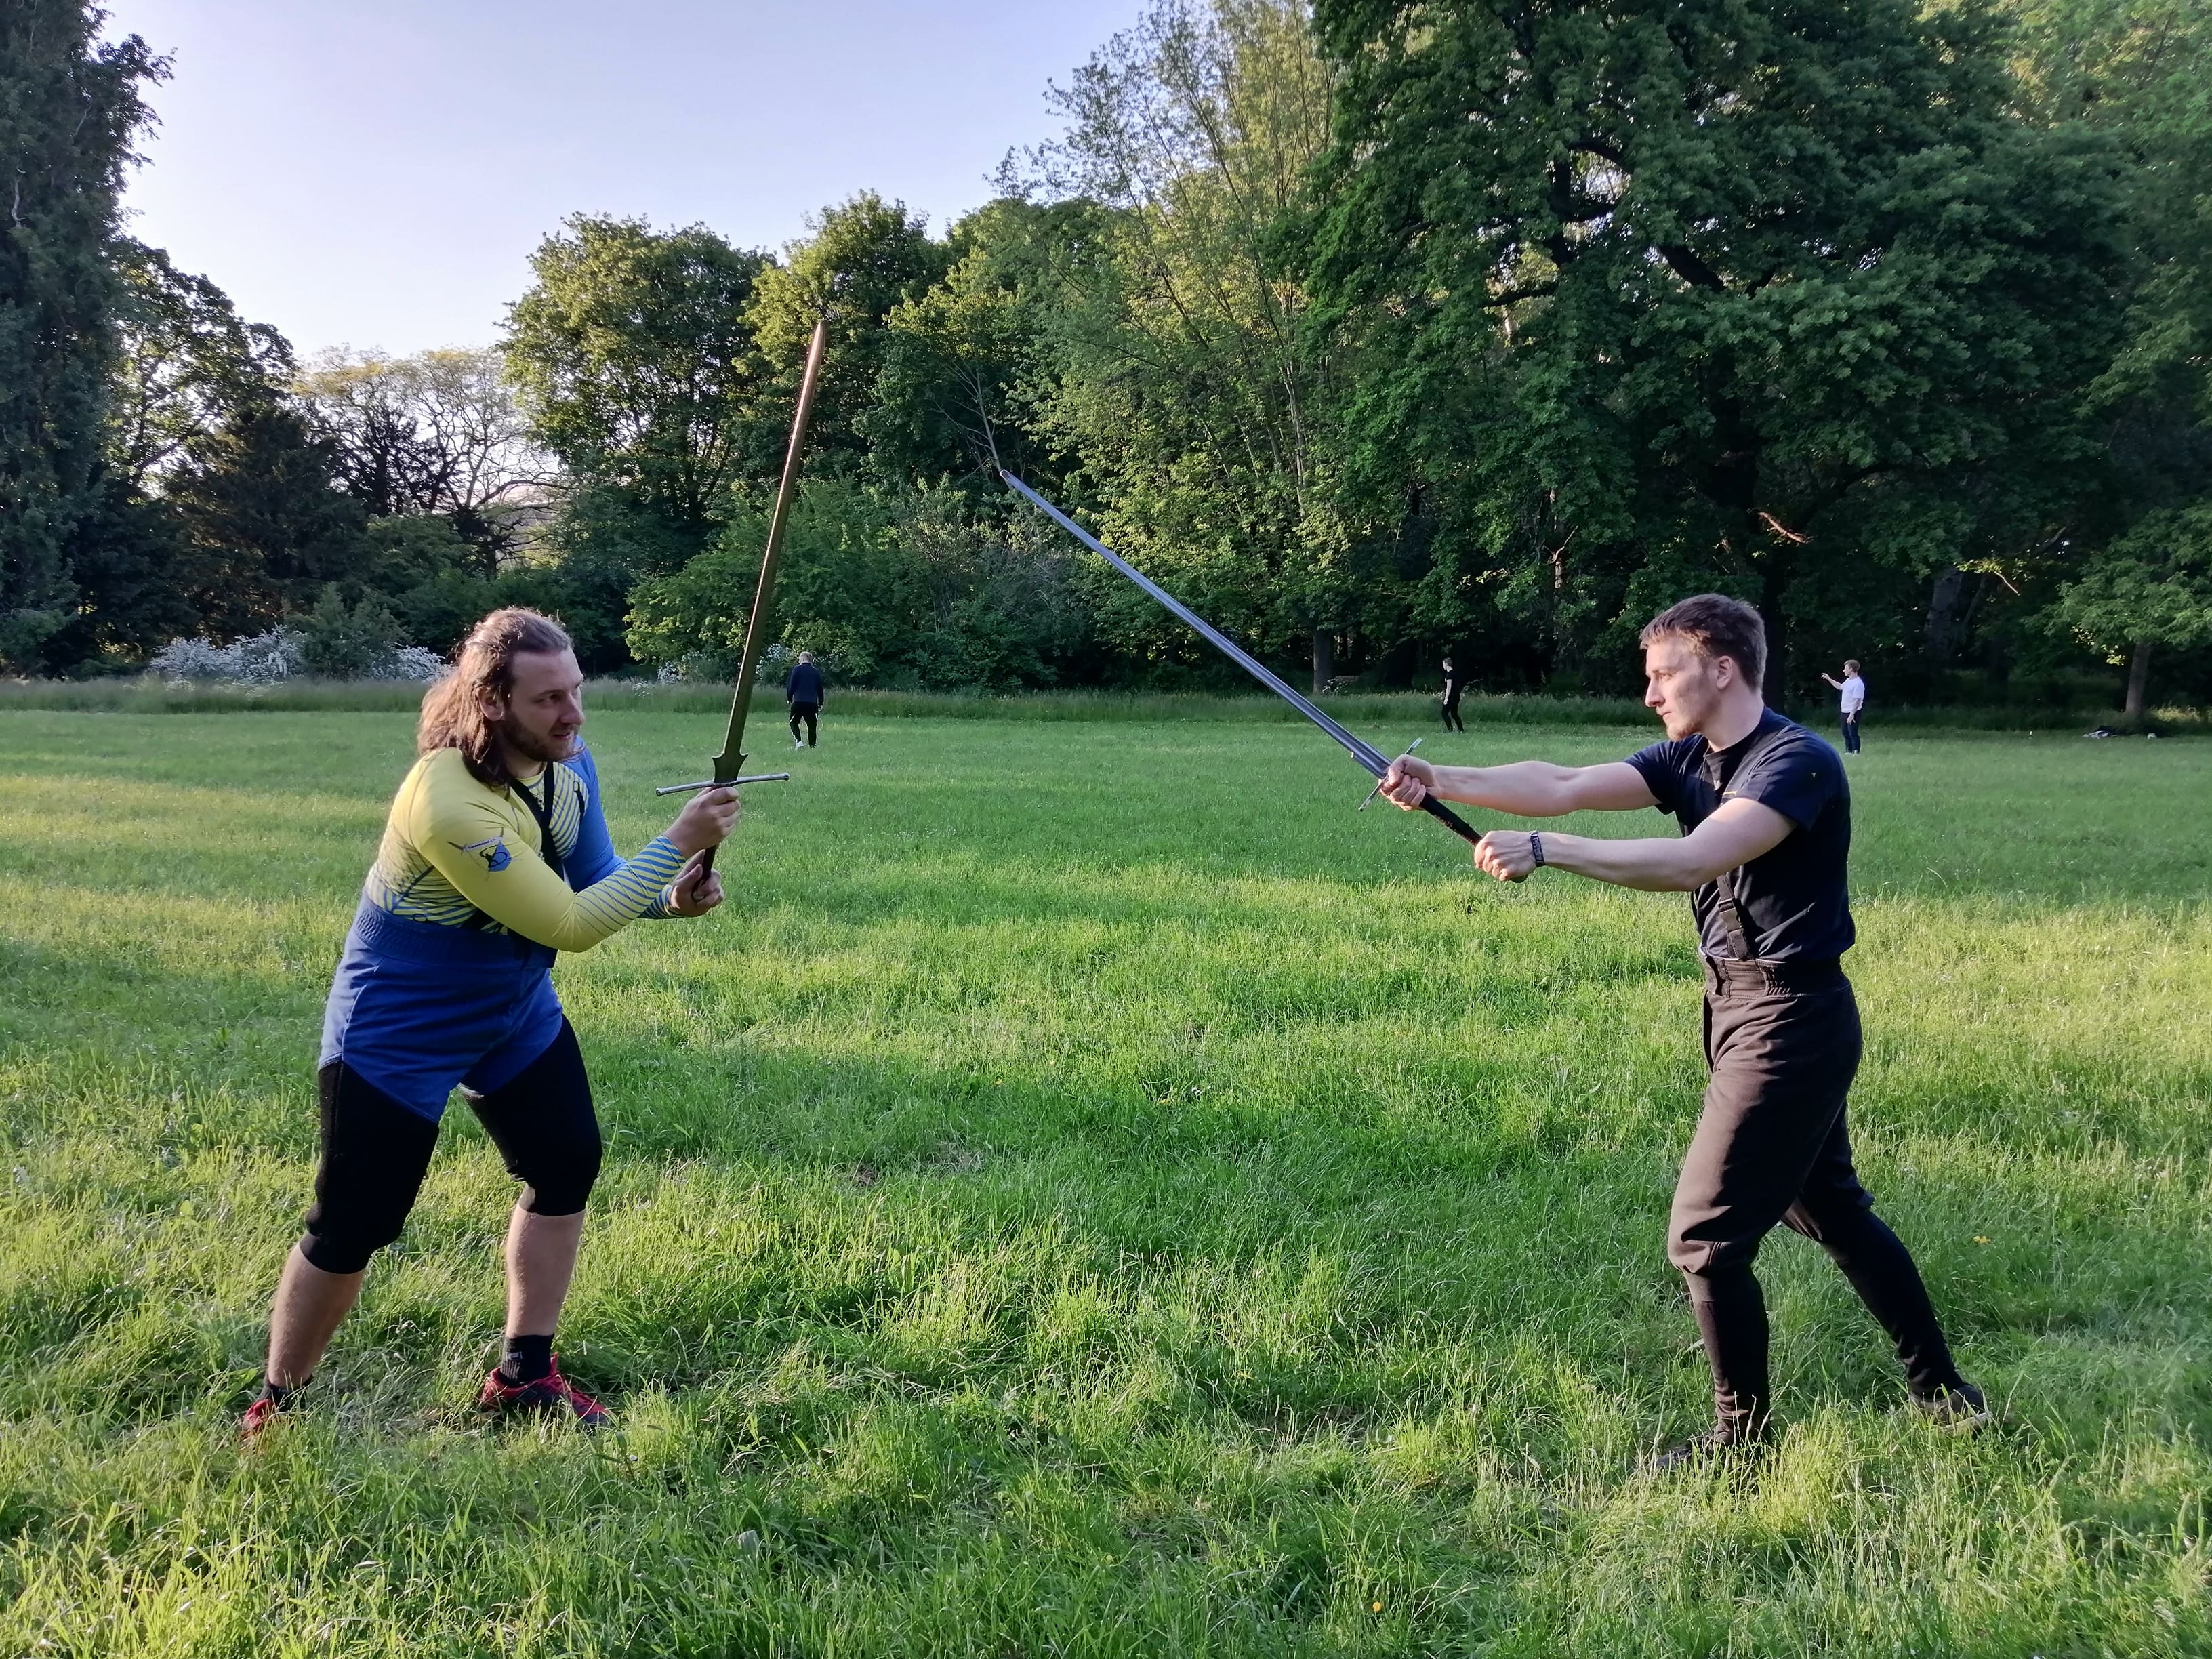
\includegraphics[width=\linewidth]{Oberhau3.jpg}
\endminipage\hfill
\minipage{0.24\textwidth}
    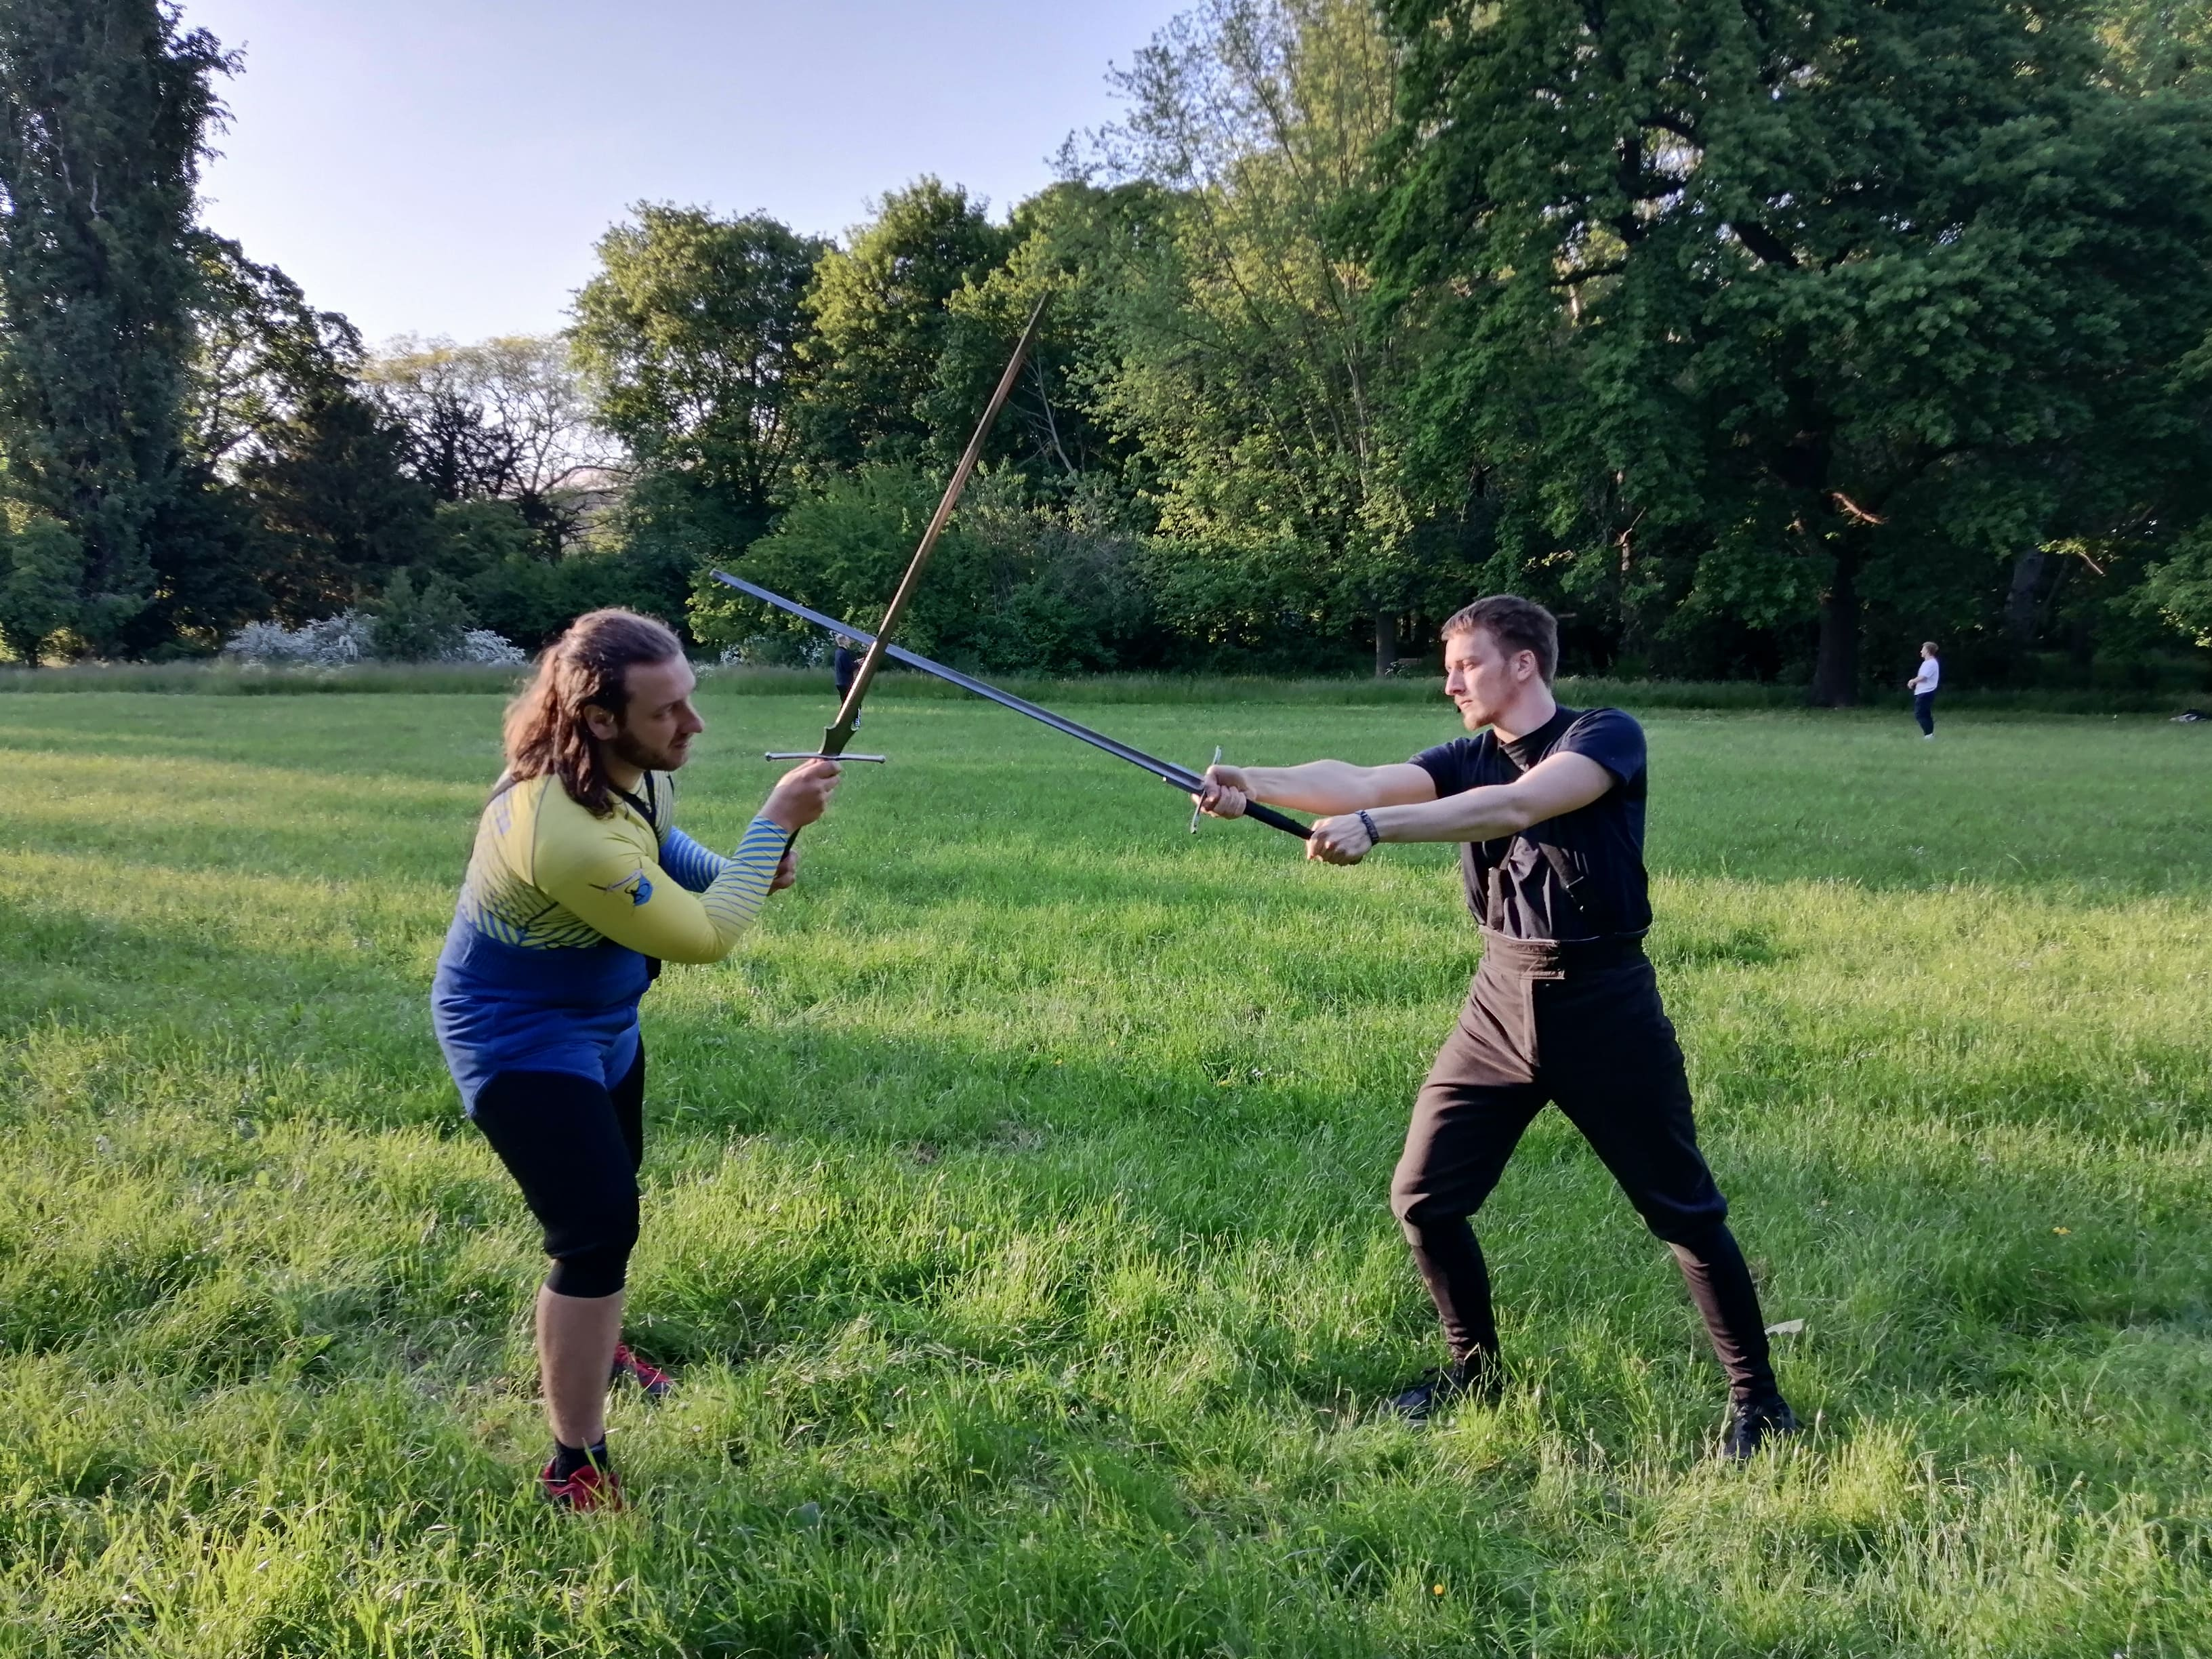
\includegraphics[width=\linewidth]{Oberhau4.jpg}
\endminipage
\end{figure}

\FloatBarrier
\hrule
\hfill
\\
Unterhau:

\FloatBarrier

\begin{figure}[!htb]
\minipage{0.24\textwidth}
    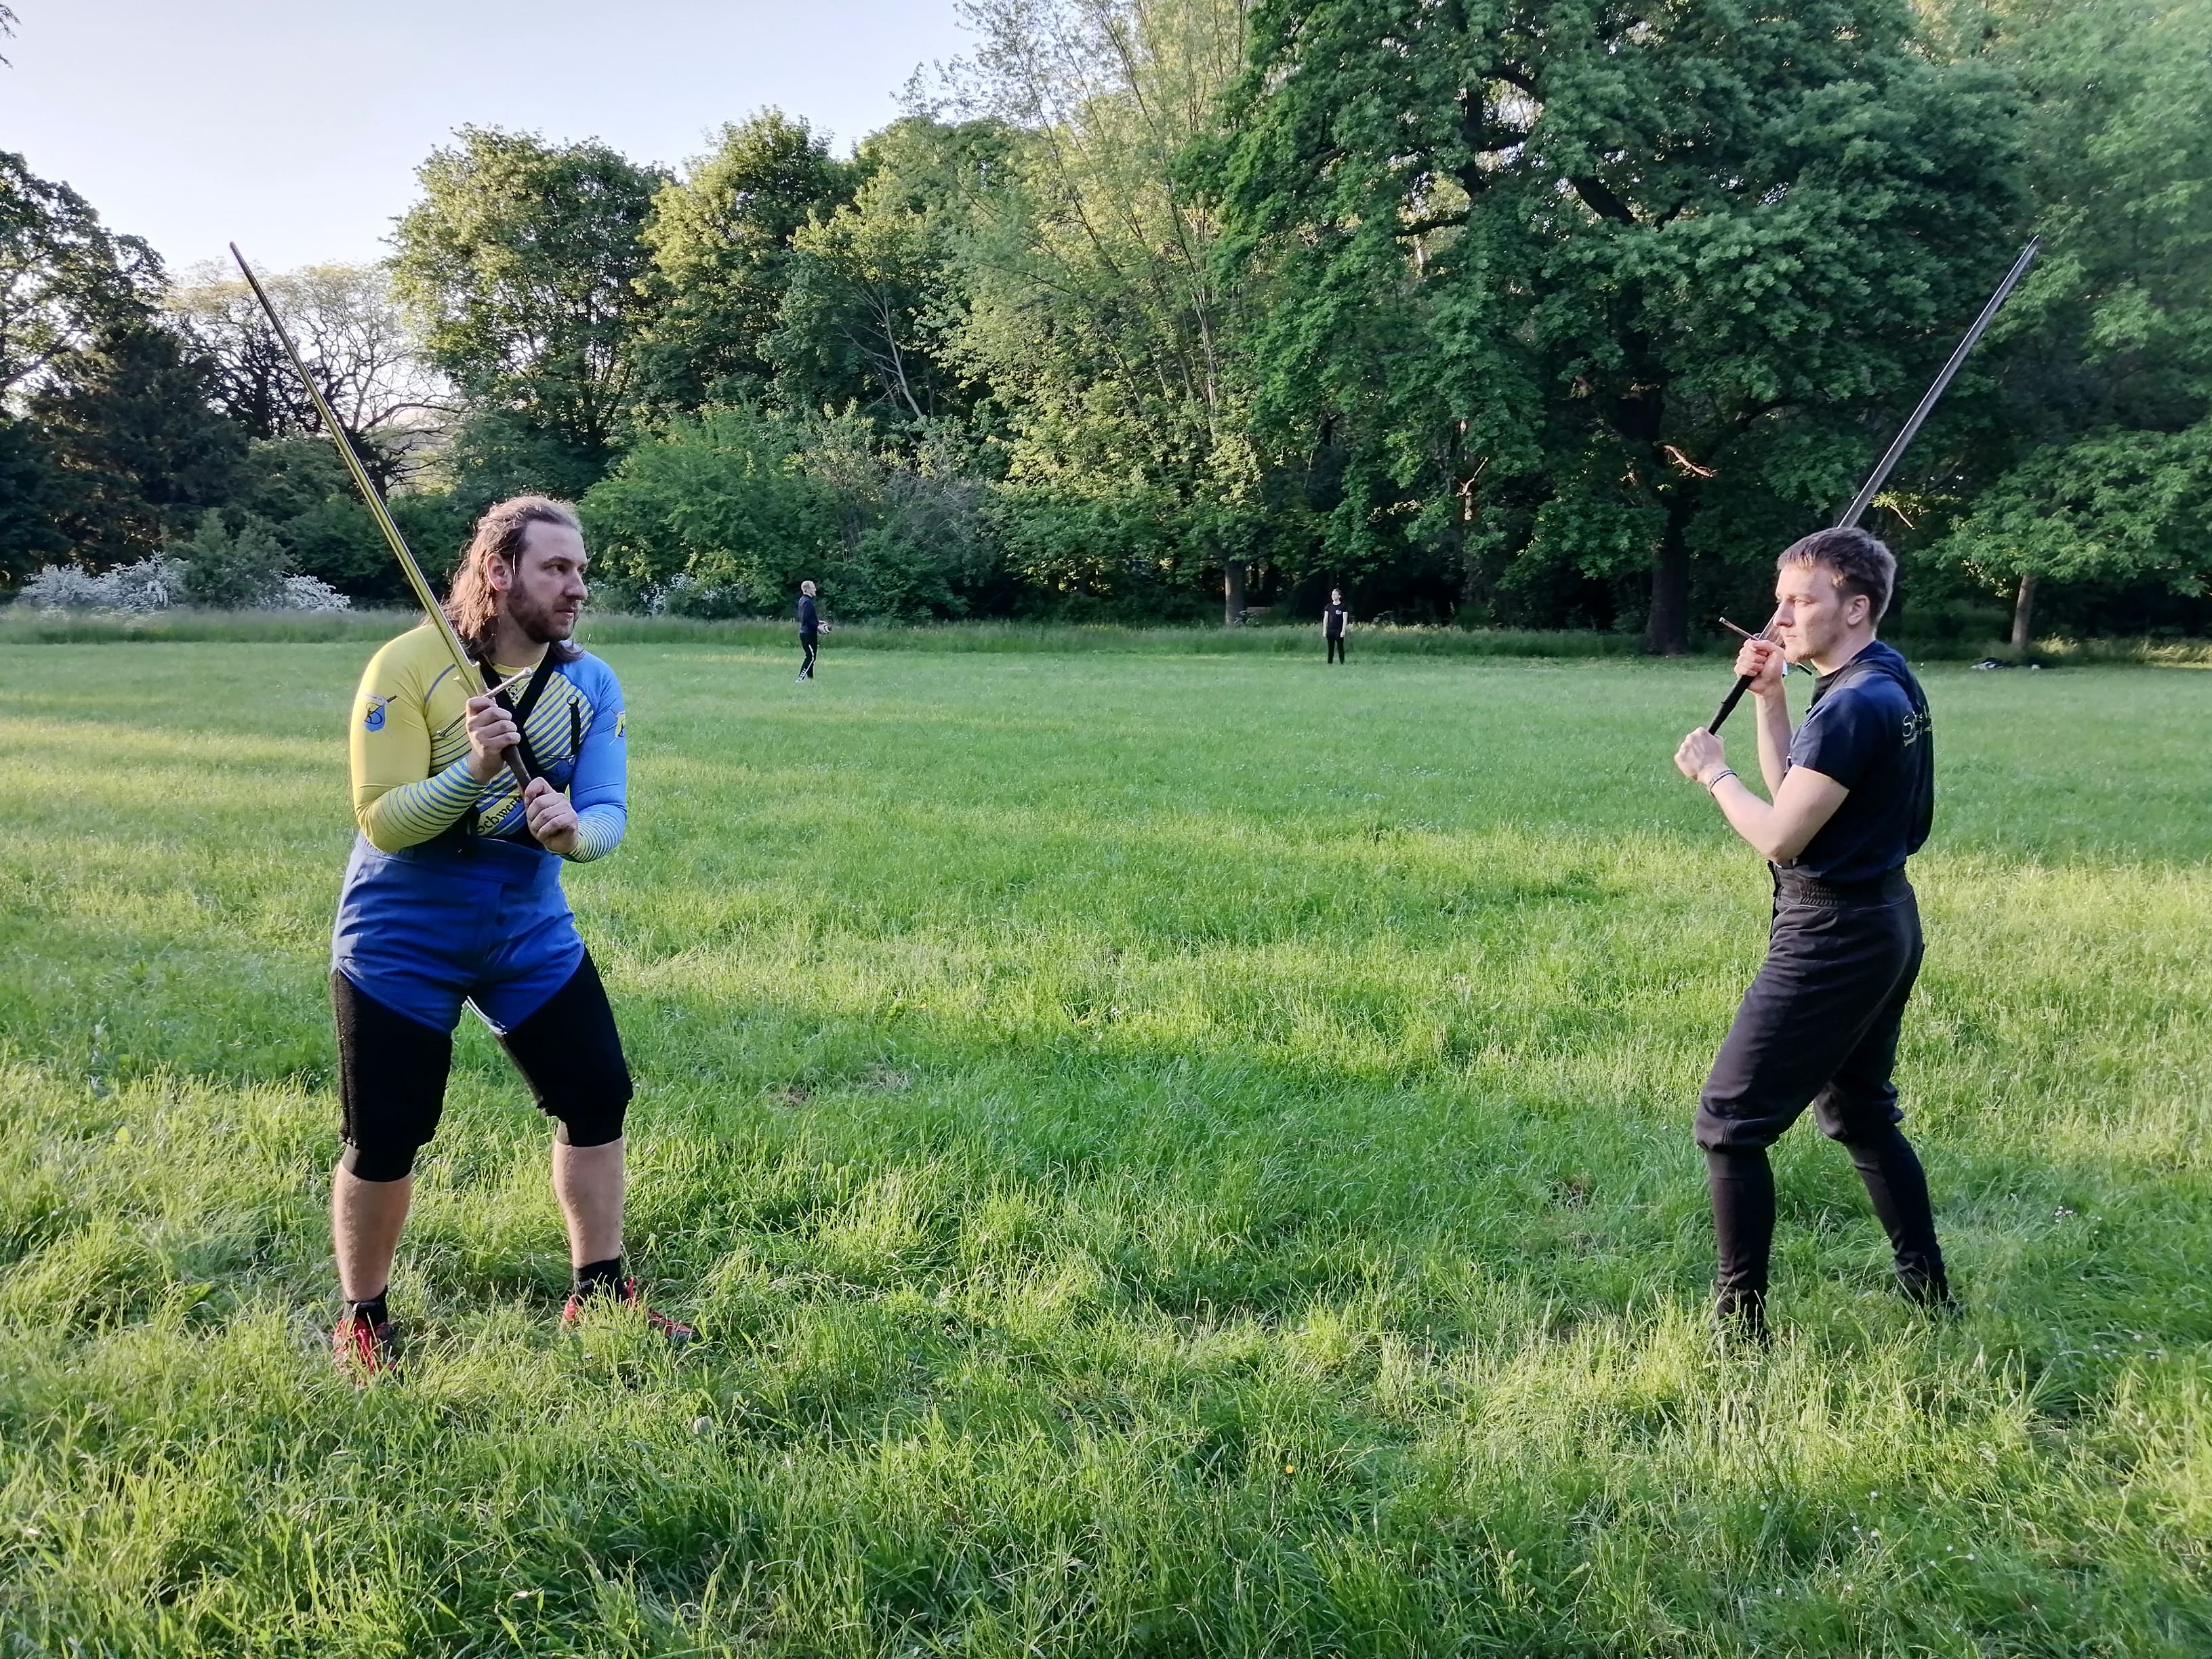
\includegraphics[width=\linewidth]{Unterhau1.jpg}
\endminipage\hfill
\minipage{0.24\textwidth}
    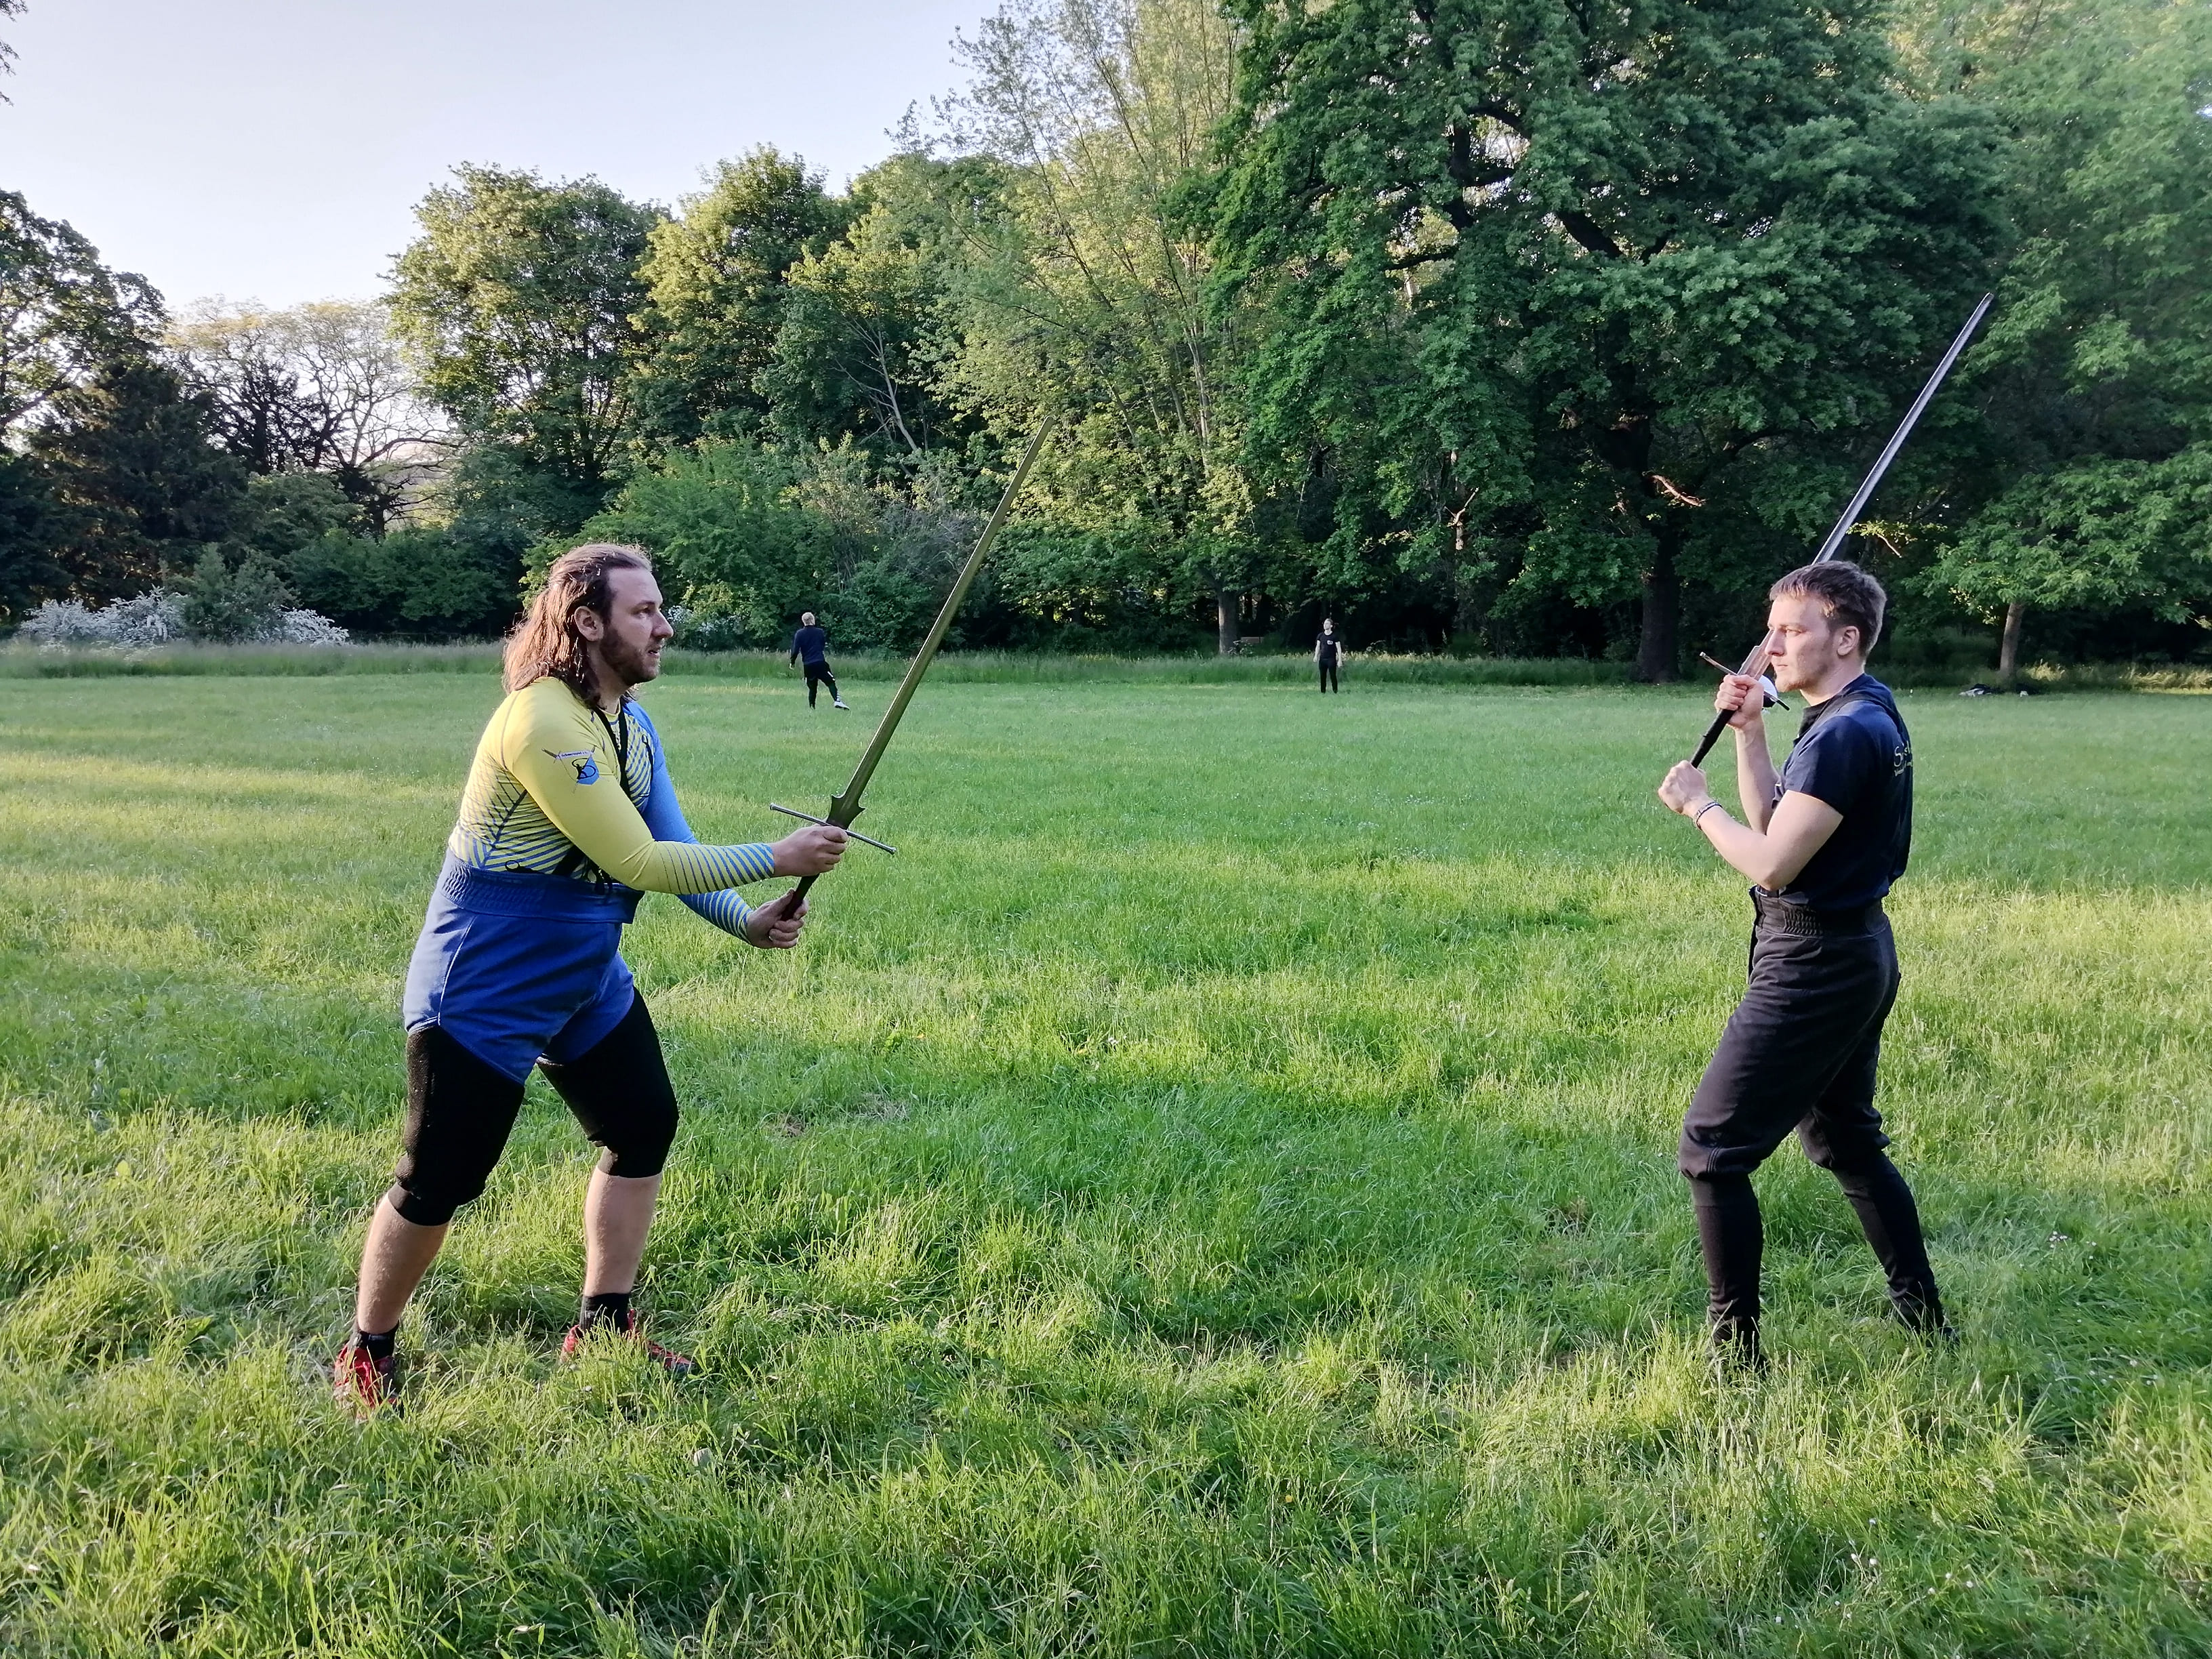
\includegraphics[width=\linewidth]{Unterhau2.jpg}
\endminipage\hfill
\minipage{0.24\textwidth}
    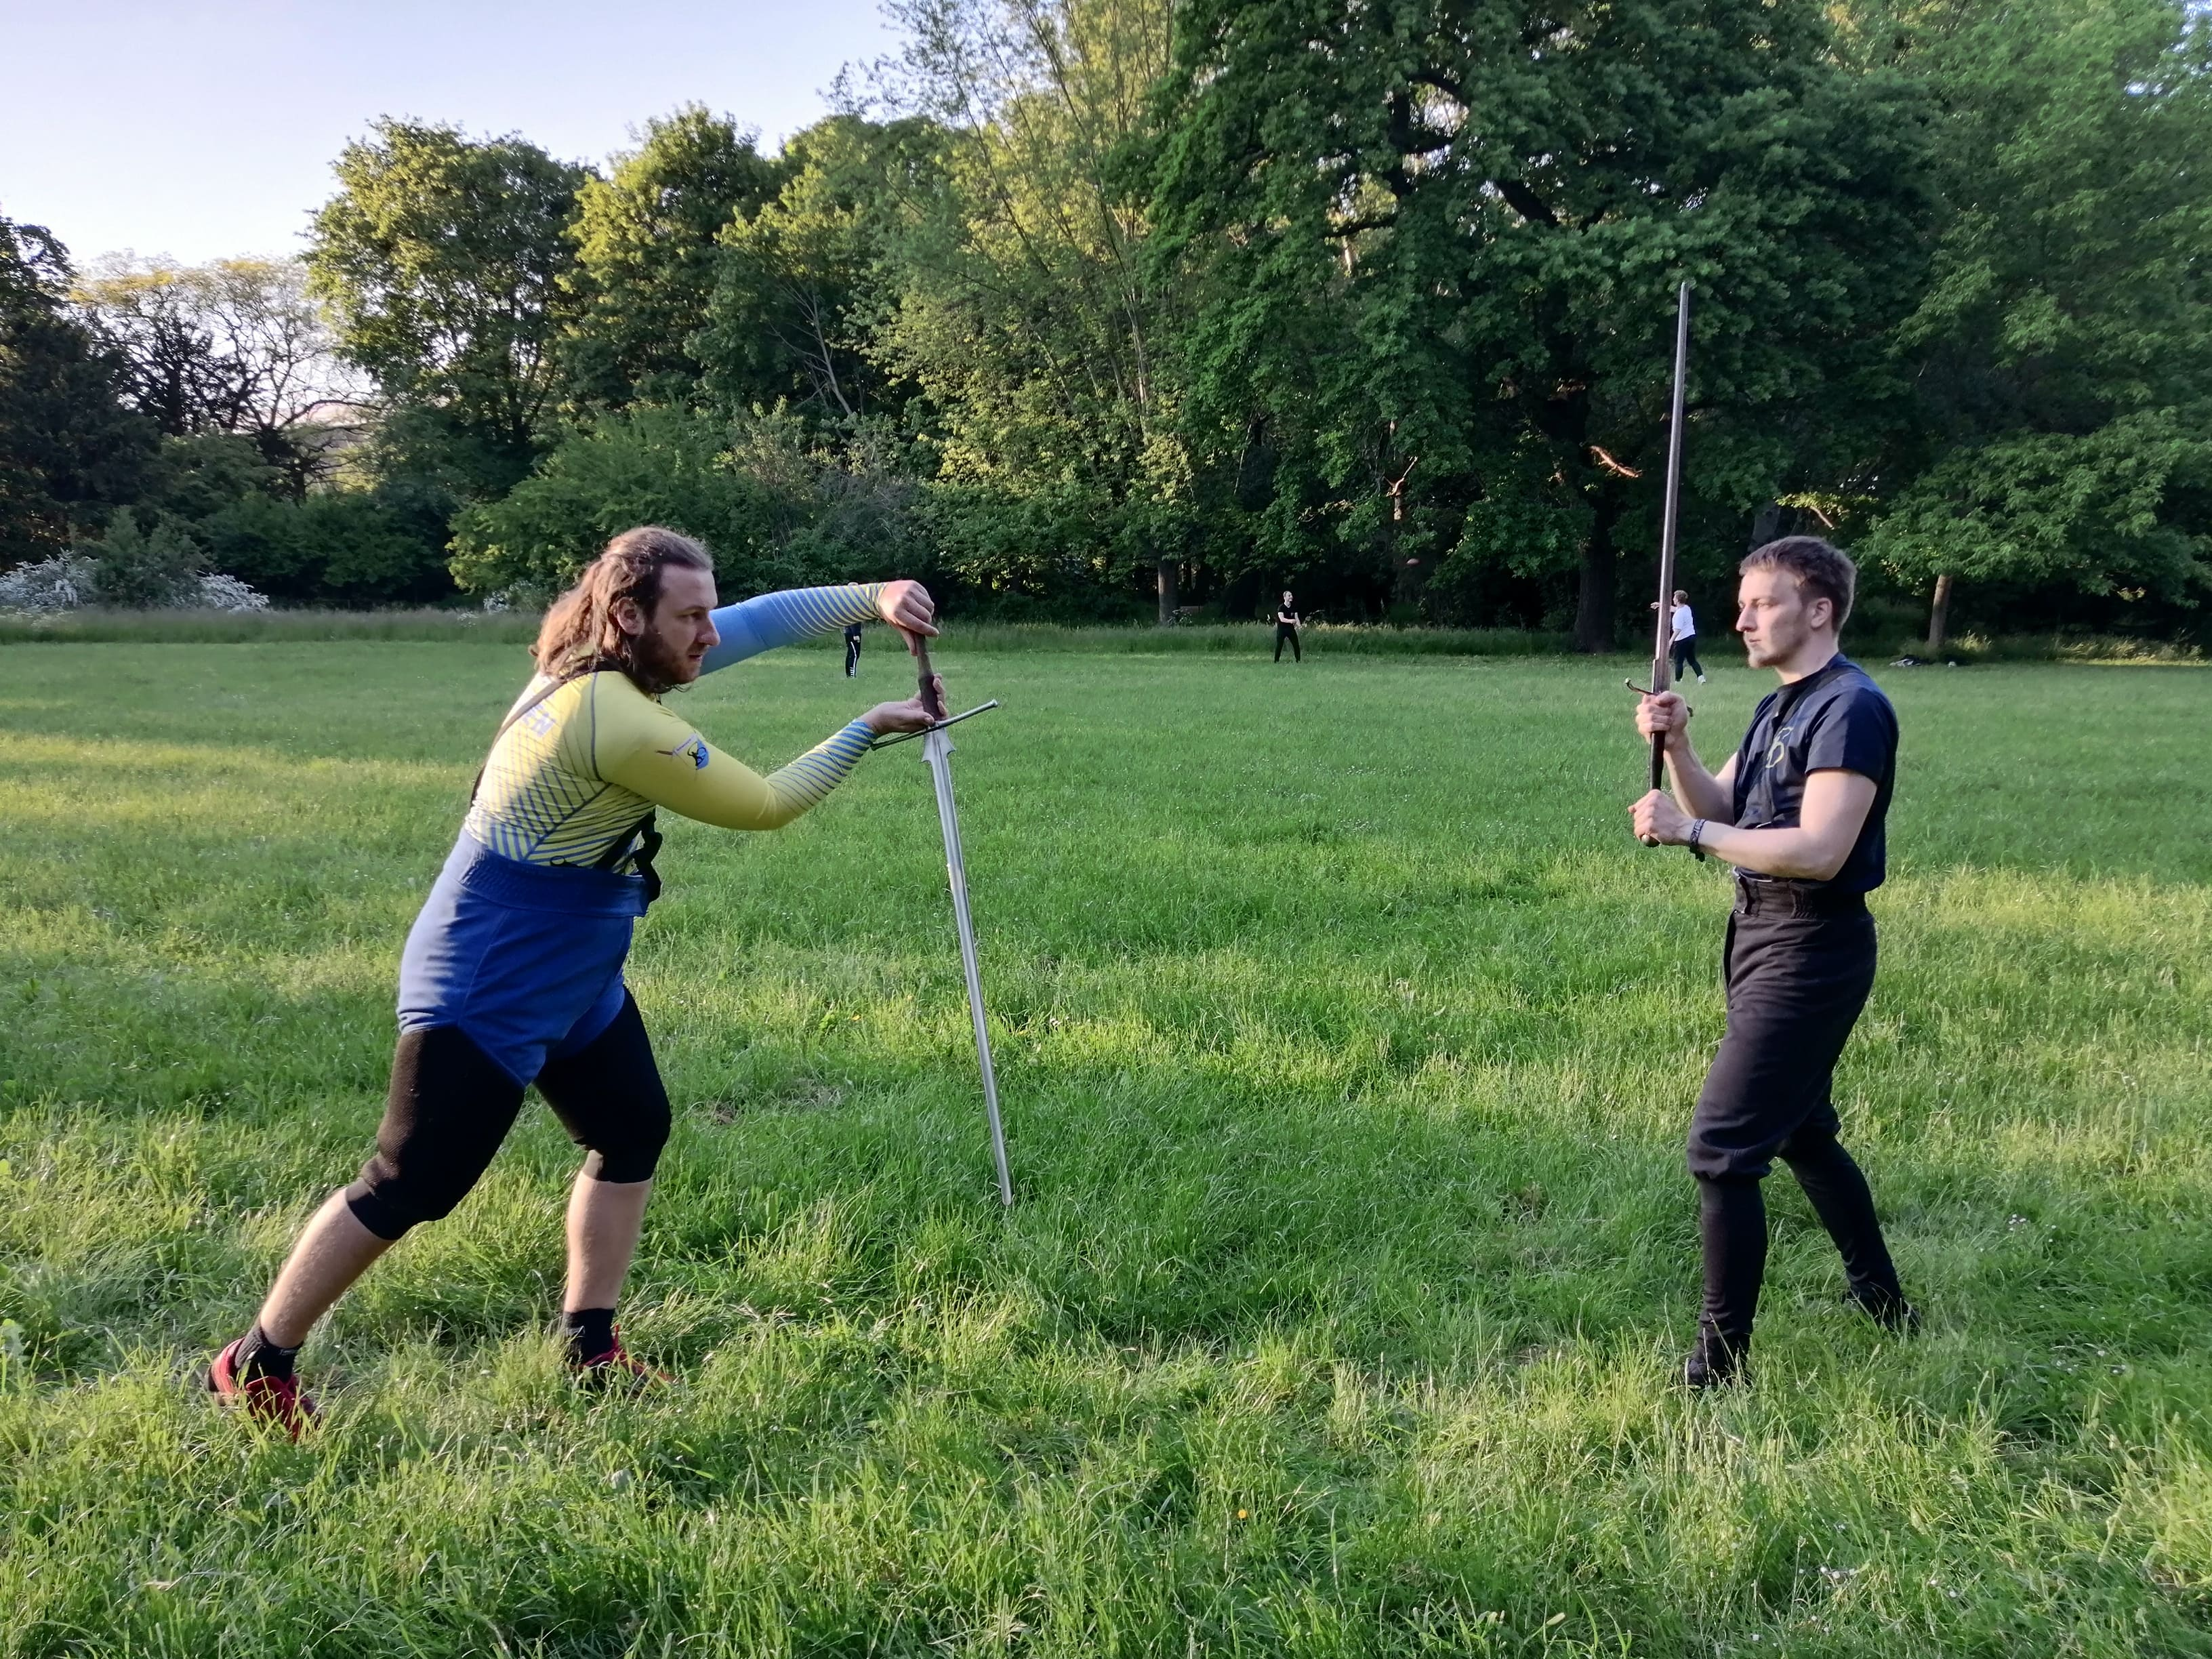
\includegraphics[width=\linewidth]{Unterhau3.jpg}
\endminipage\hfill
\minipage{0.24\textwidth}%
    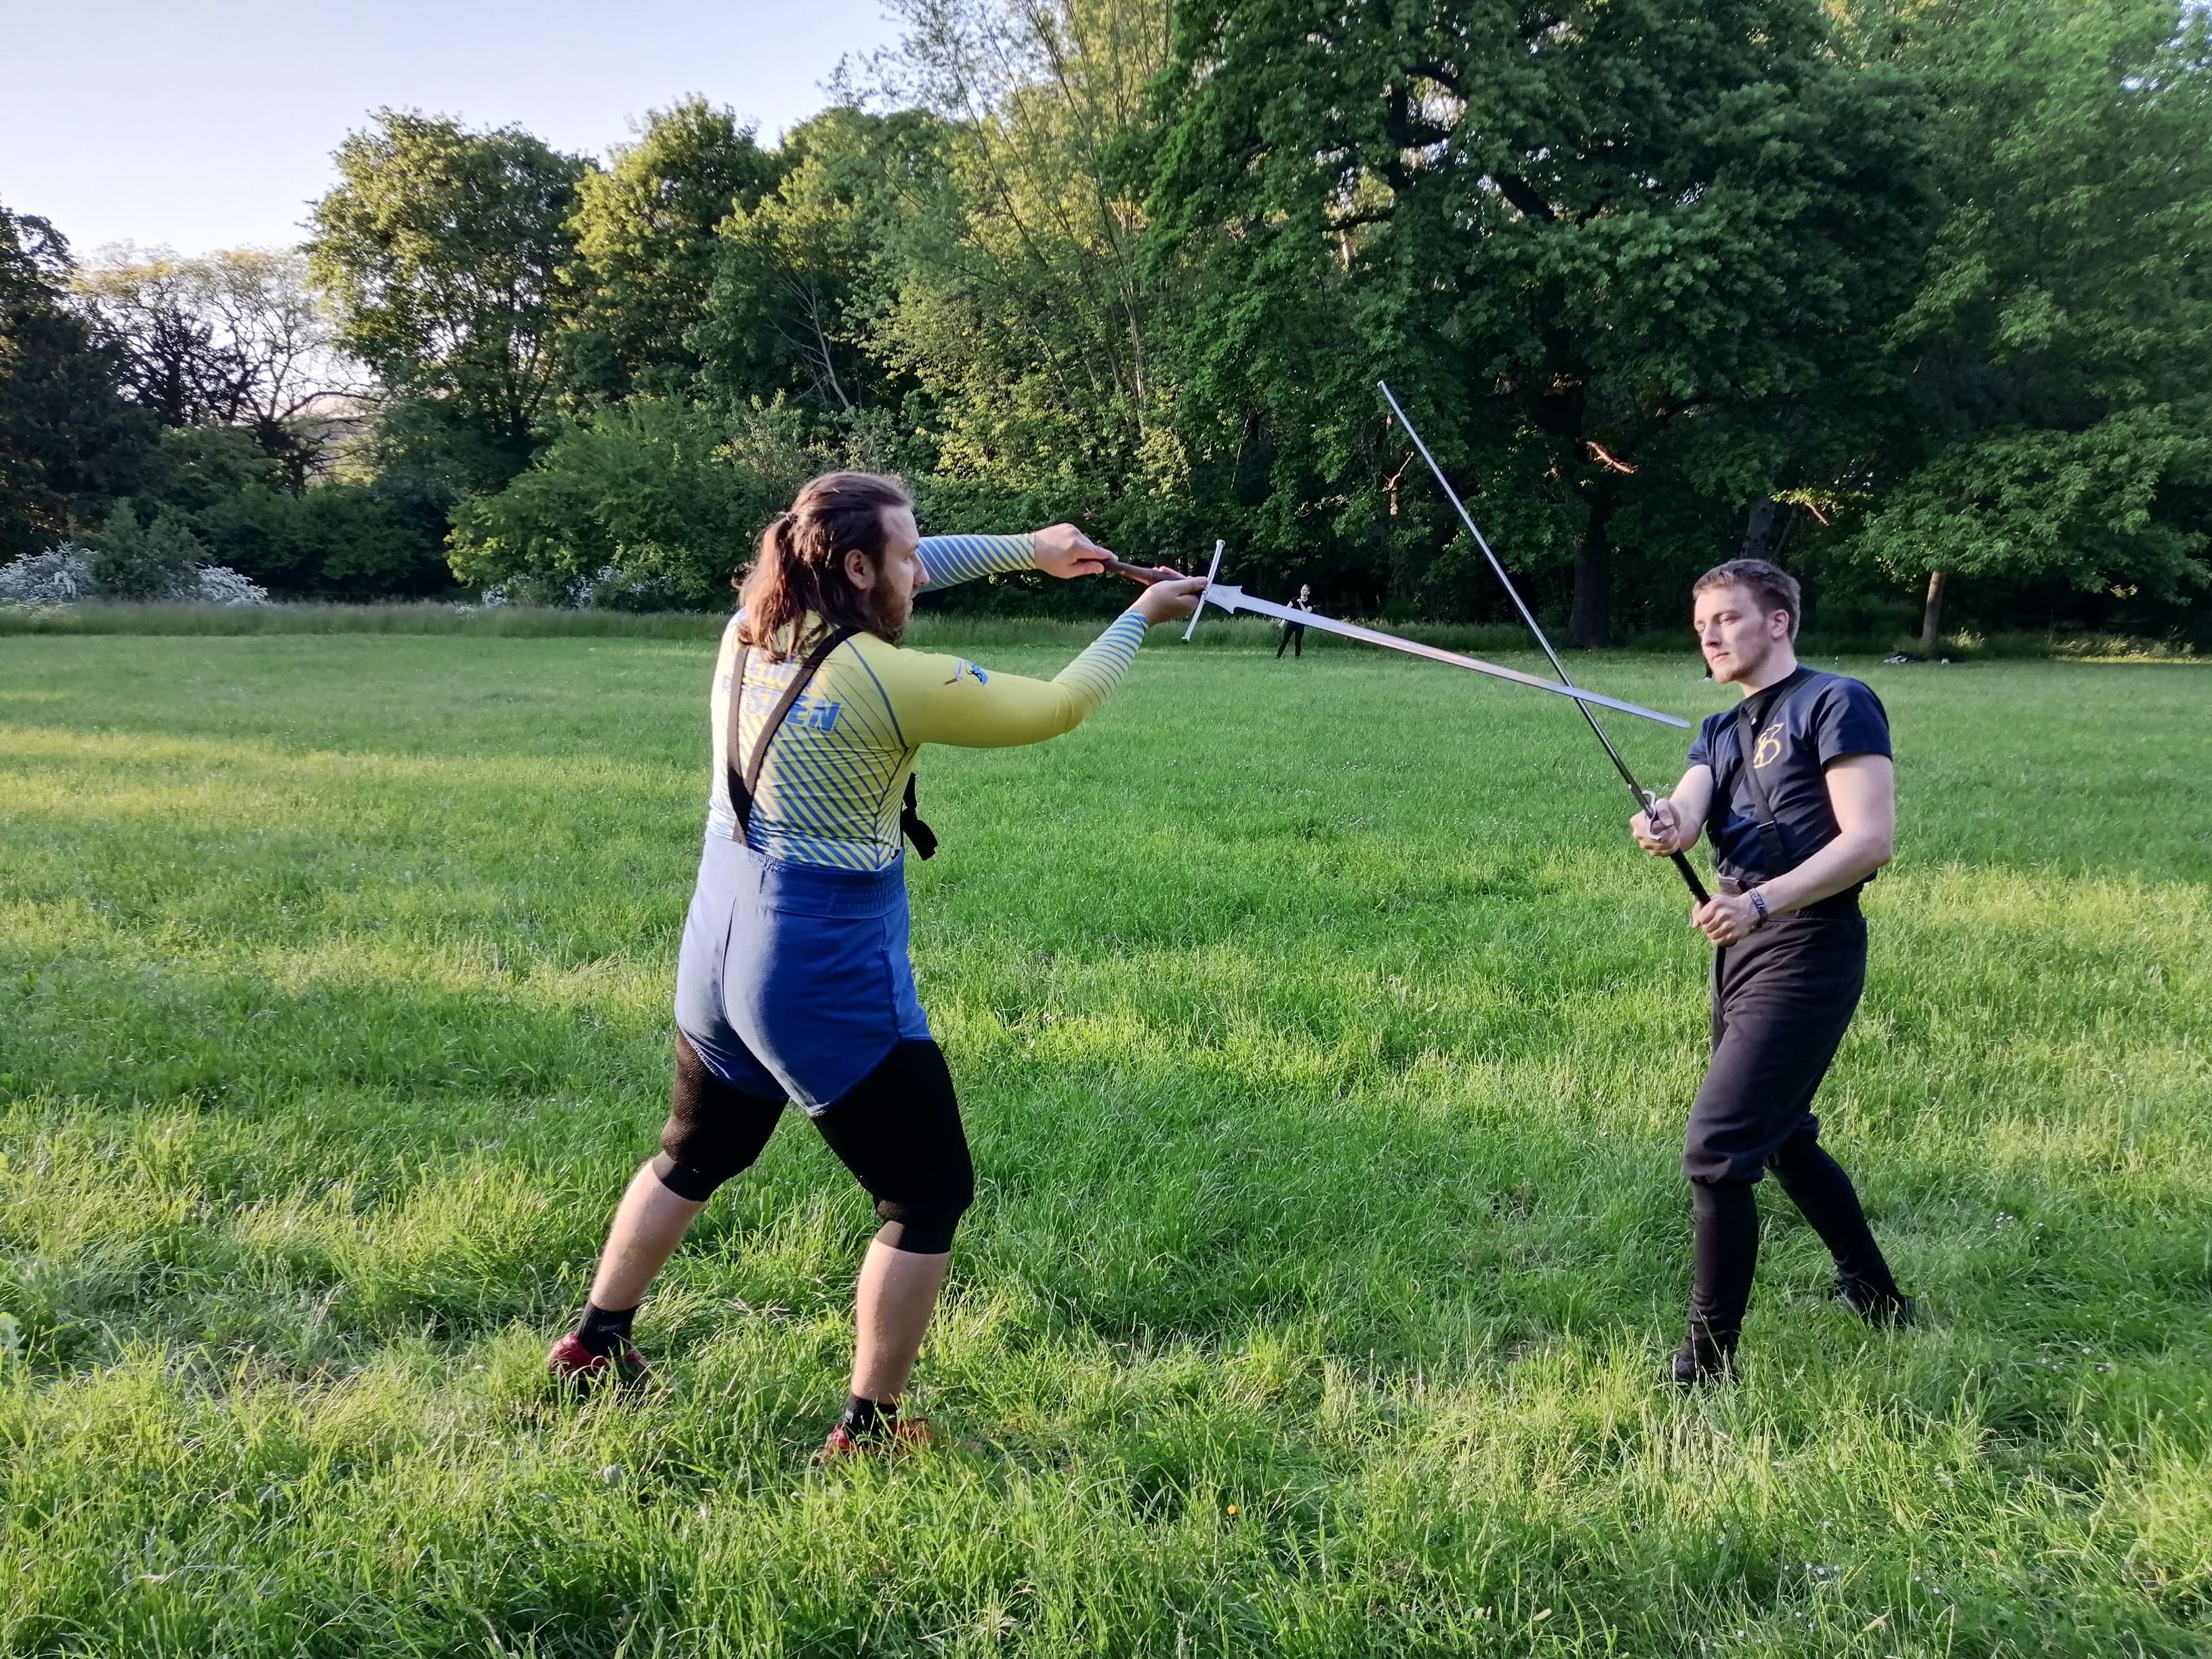
\includegraphics[width=\linewidth]{Unterhau4.jpg}
\endminipage
\end{figure}

\FloatBarrier

\paragraph{Stiche}

Stiche haben im Vergleich zu Häuen eine leicht erhöhte Reichweite und können nicht passiv gedeckt werden. Ein effektiver Stich erfordert im Vergleich zu einem Hau noch weniger Kraft. Der Nachteil an Stichen ist, dass es mit ihnen schwerer ist, Selbstschutz herzustellen.

\paragraph{Schnitte}

Schnitte besitzen bei weitem die geringste Rechweite, da die Klinge bereits auf ihrem Ziel aufliegen muss, damit ein Schnitt initiiert werden kann. Schnitte sind deshalb praktisch für enge Mensuren. Sie können Selbstschutz herstellen, indem entweder die Klinge des:der Gegner:in durch den eigenen Körper blockiert wird oder man den Schnitt gegen die Arme des:der Gegner:in ausführt und so dessen Klinge verdrückt.
\\
\\
Unterschnitt:

\FloatBarrier

\begin{figure}[!htb]
\minipage{0.24\textwidth}
    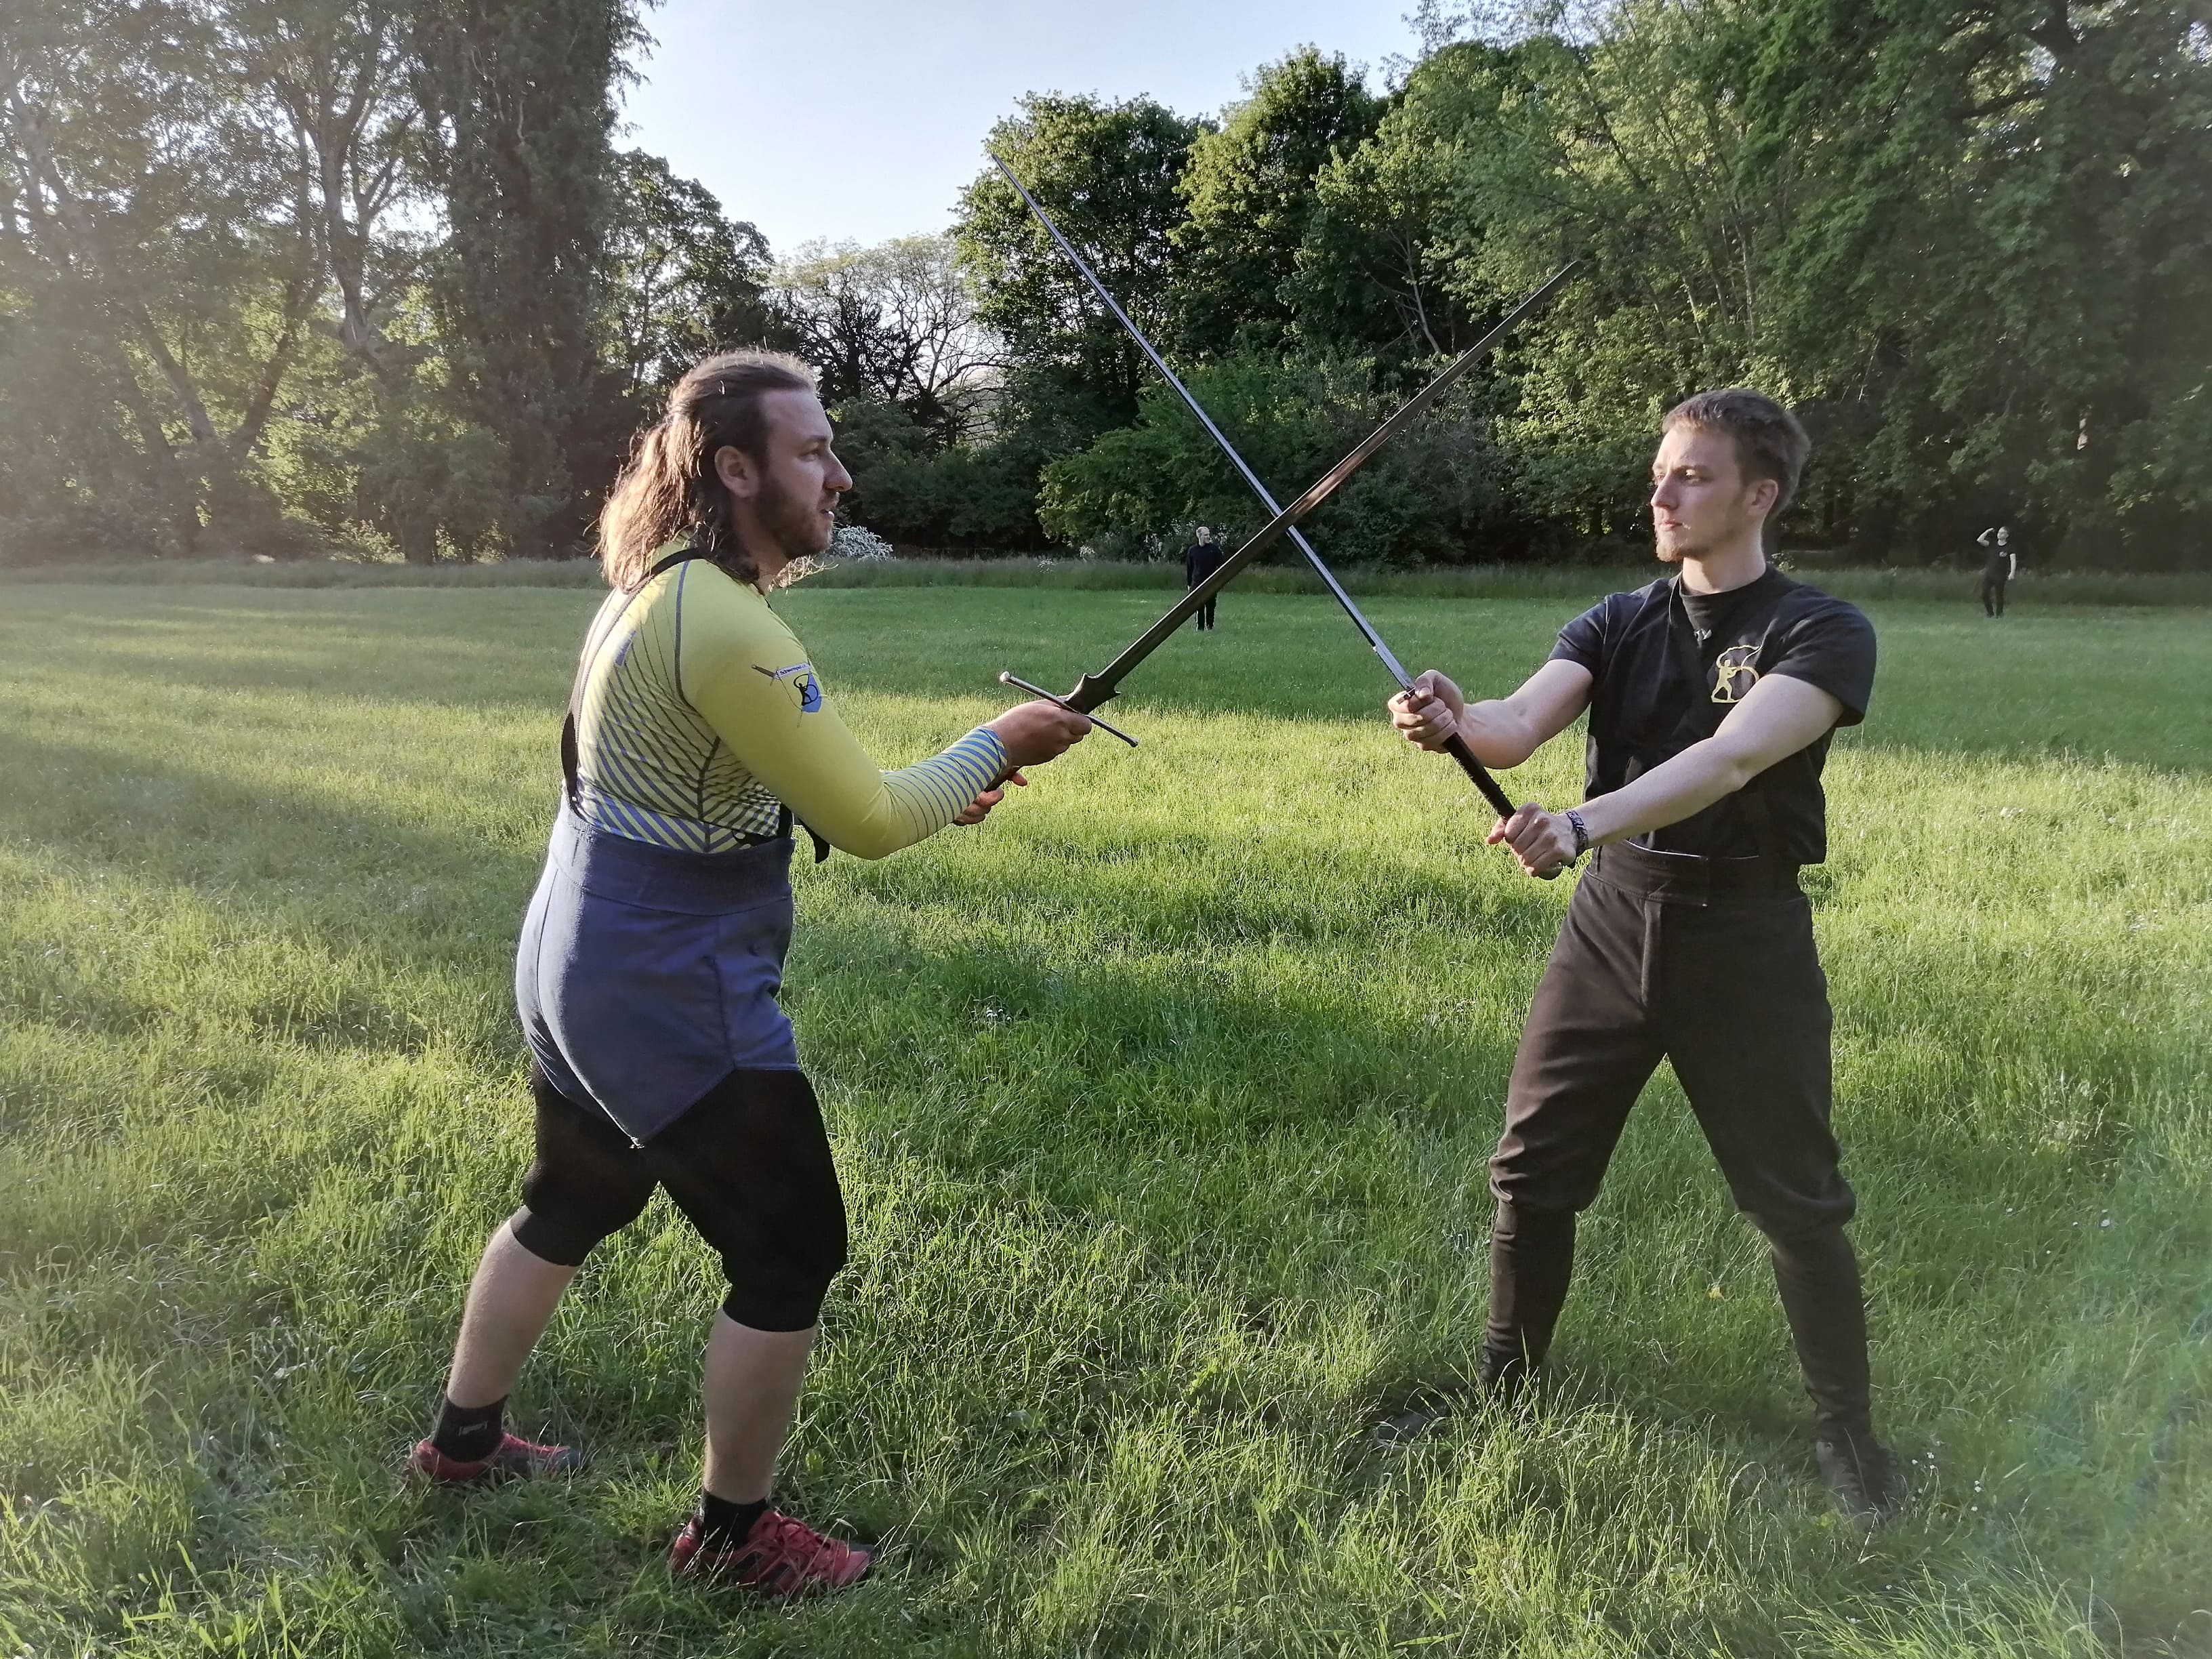
\includegraphics[width=\linewidth]{Schnitt1.jpg}
\endminipage\hfill
\minipage{0.24\textwidth}
    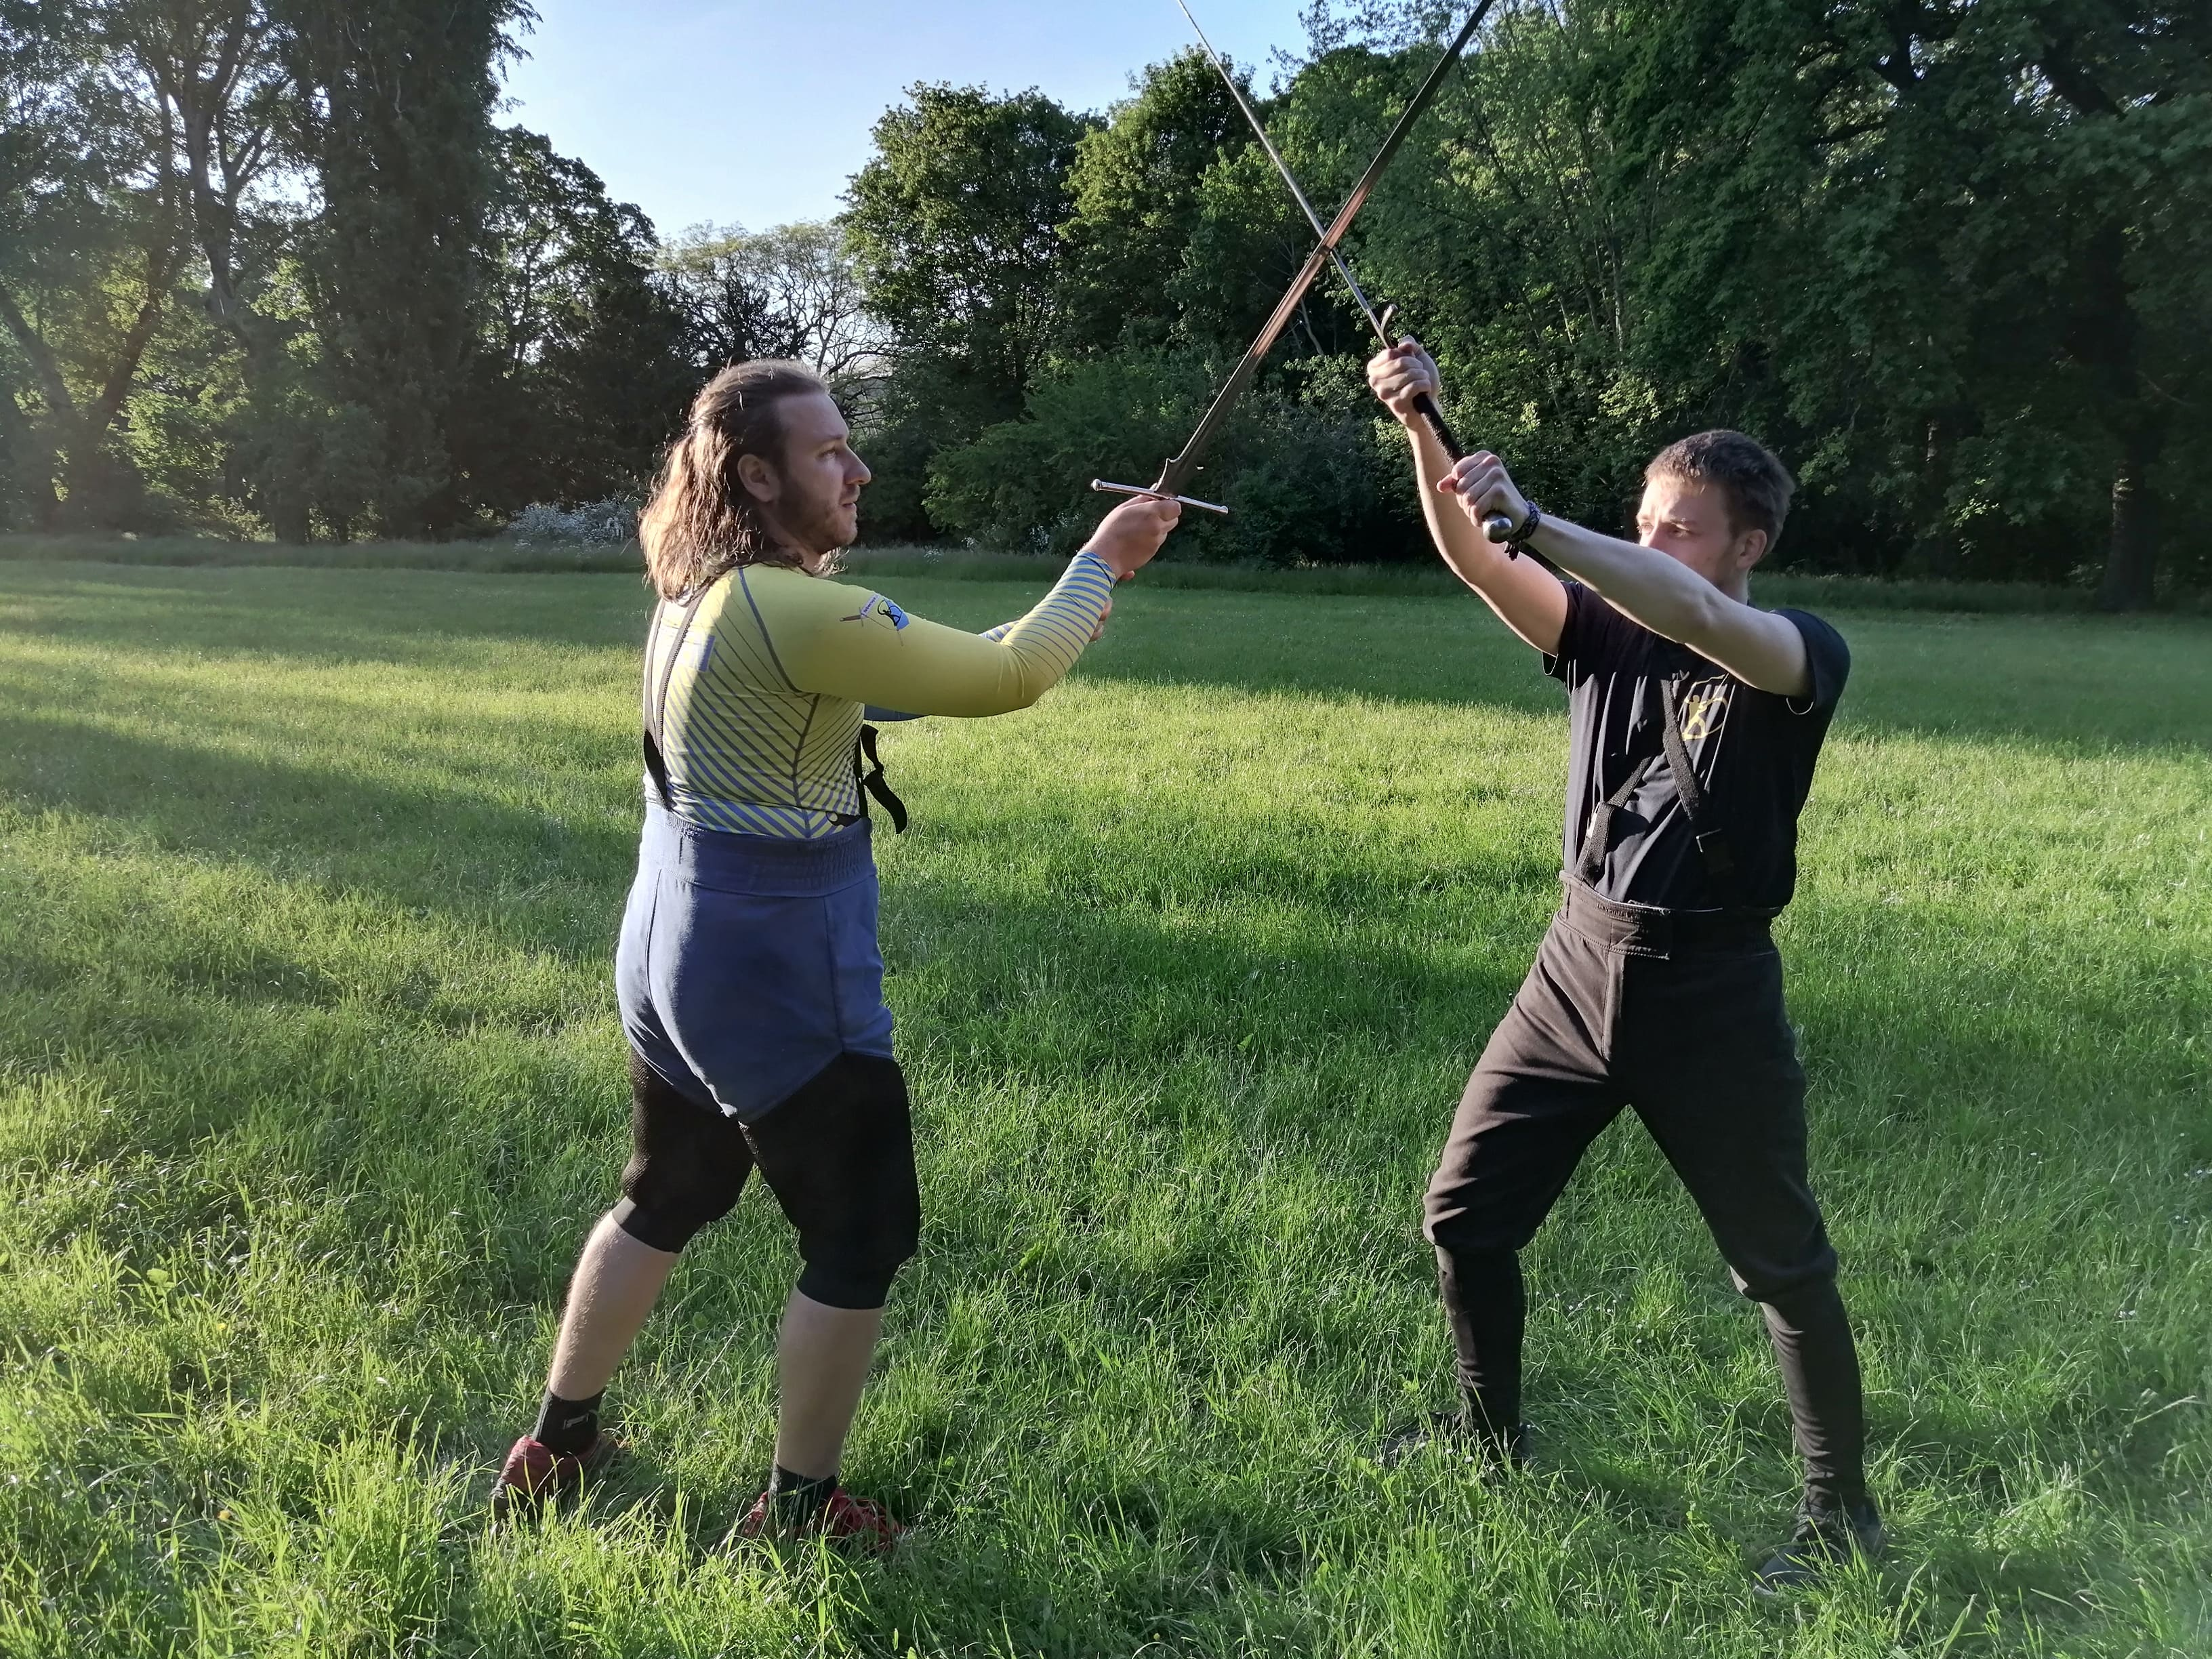
\includegraphics[width=\linewidth]{Schnitt2.jpg}
\endminipage\hfill
\minipage{0.24\textwidth}
    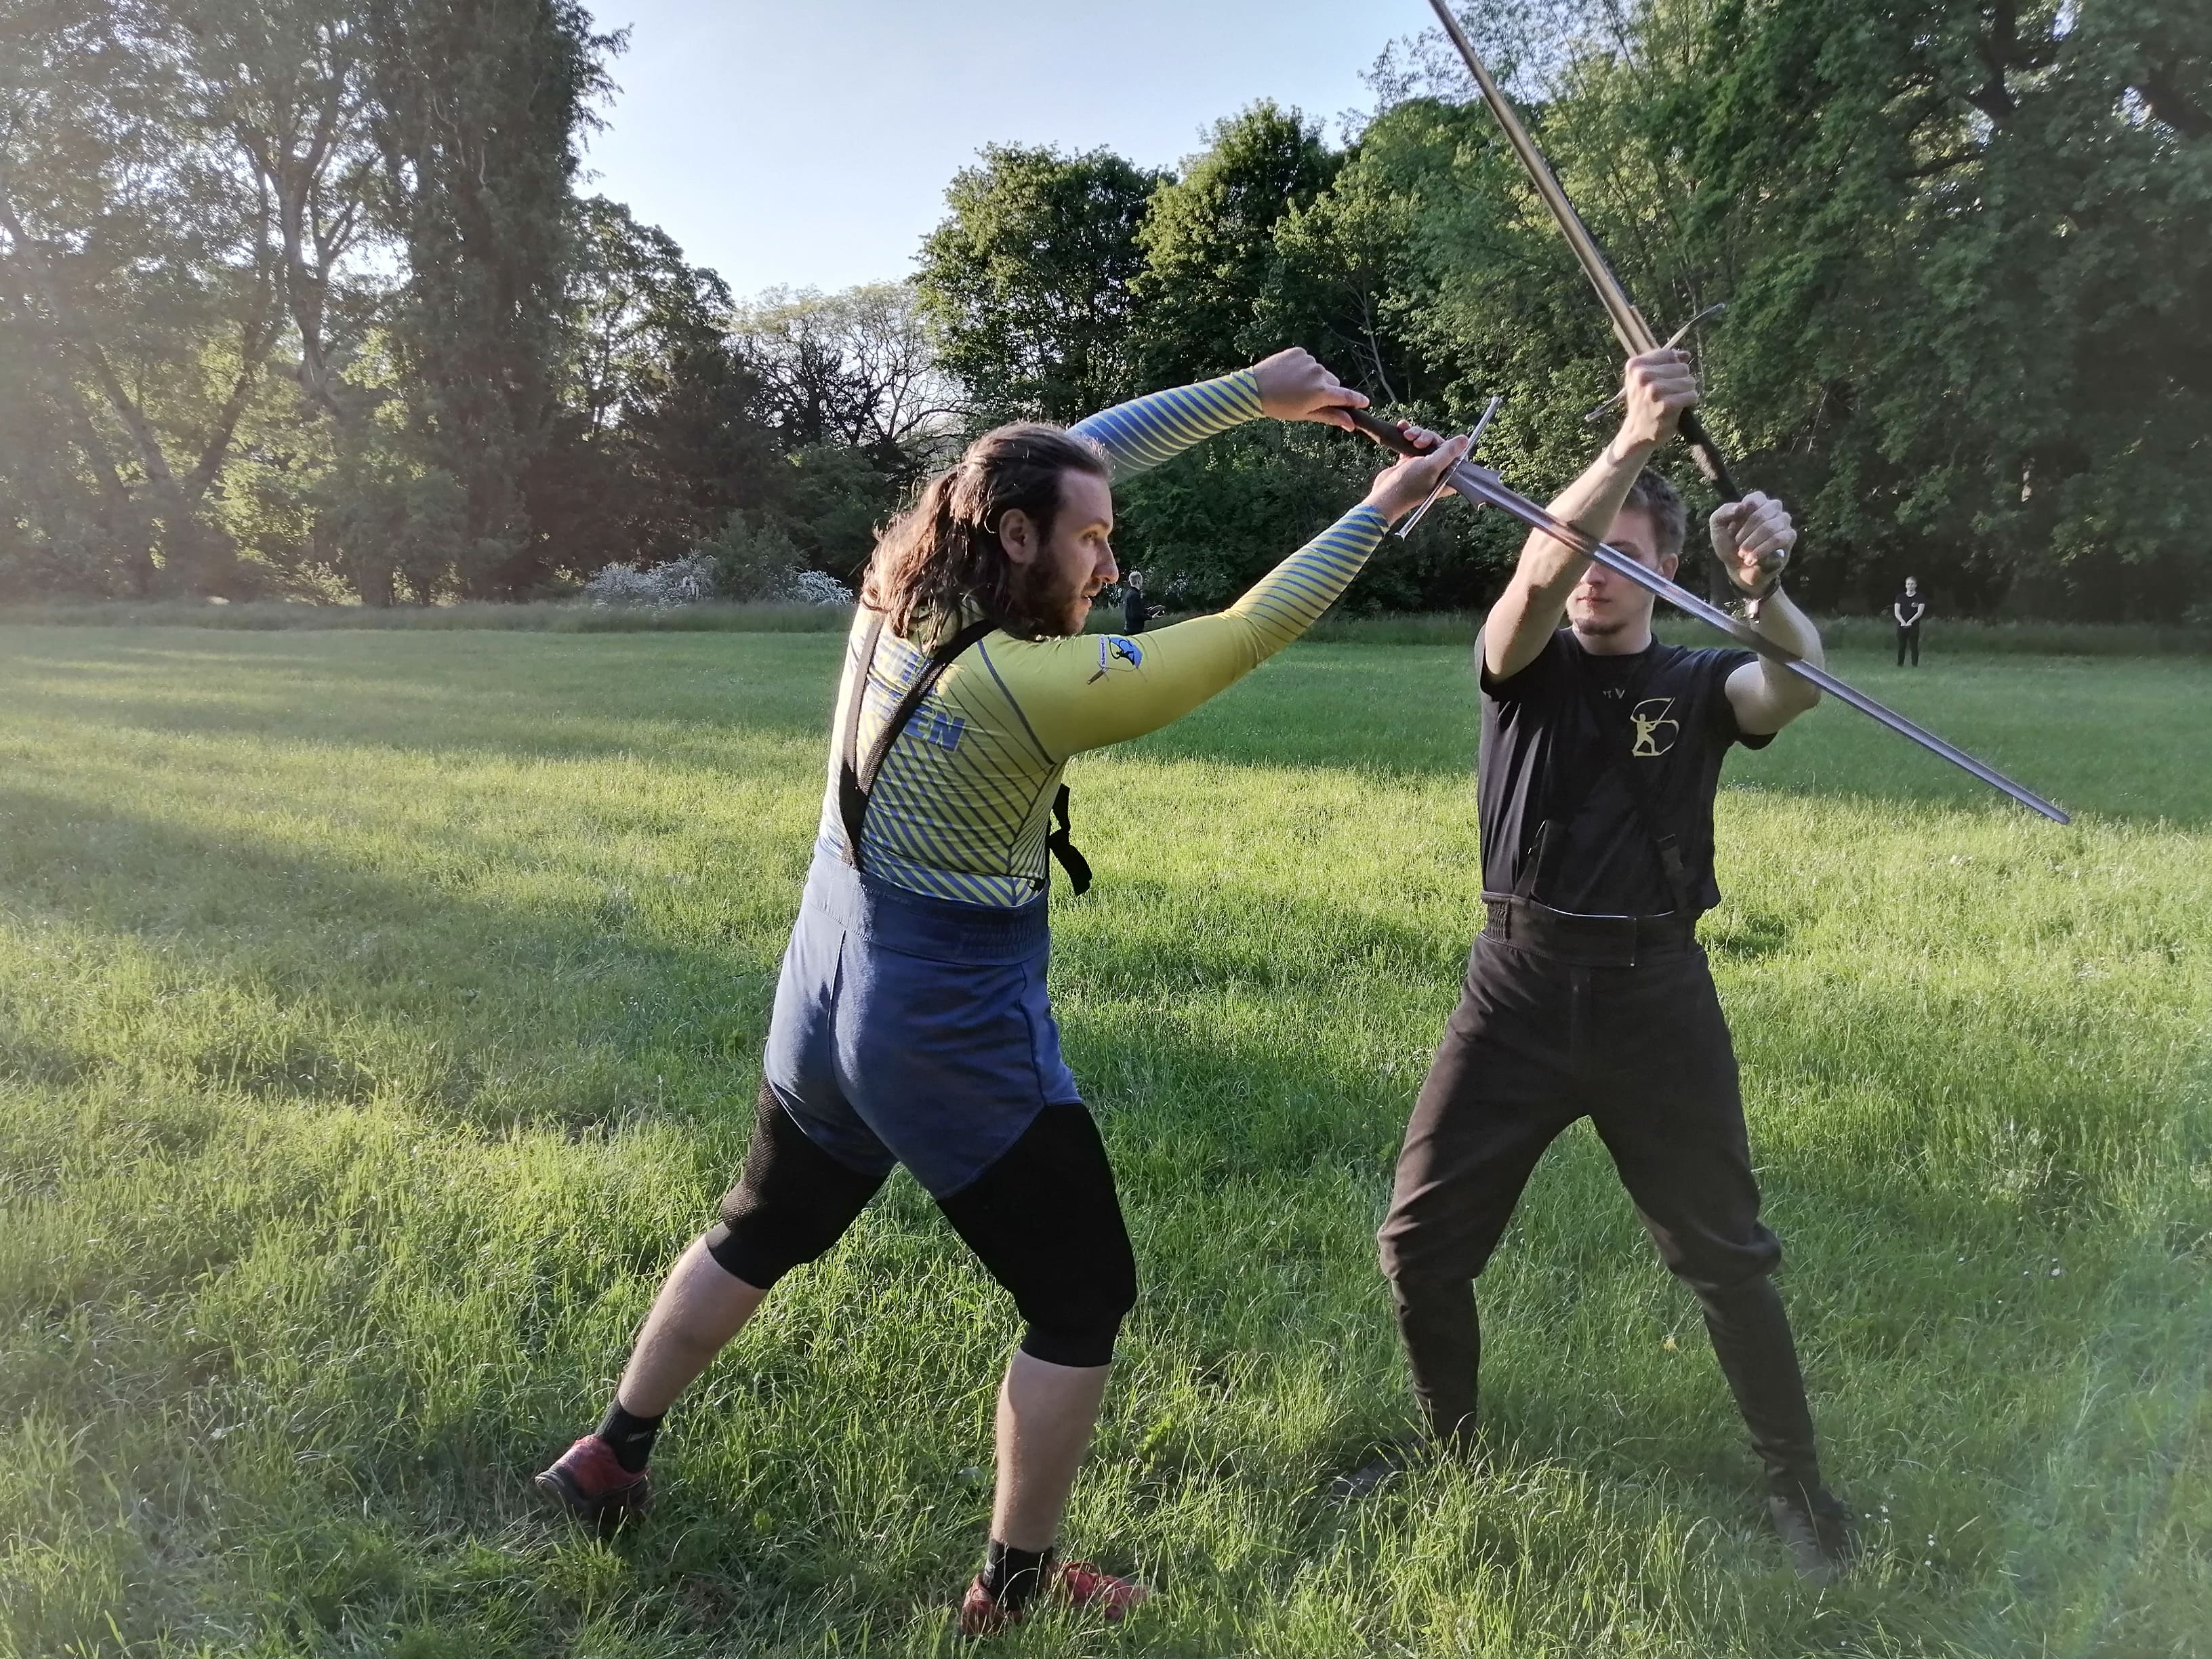
\includegraphics[width=\linewidth]{Schnitt3.jpg}
\endminipage\hfill
\minipage{0.24\textwidth}
    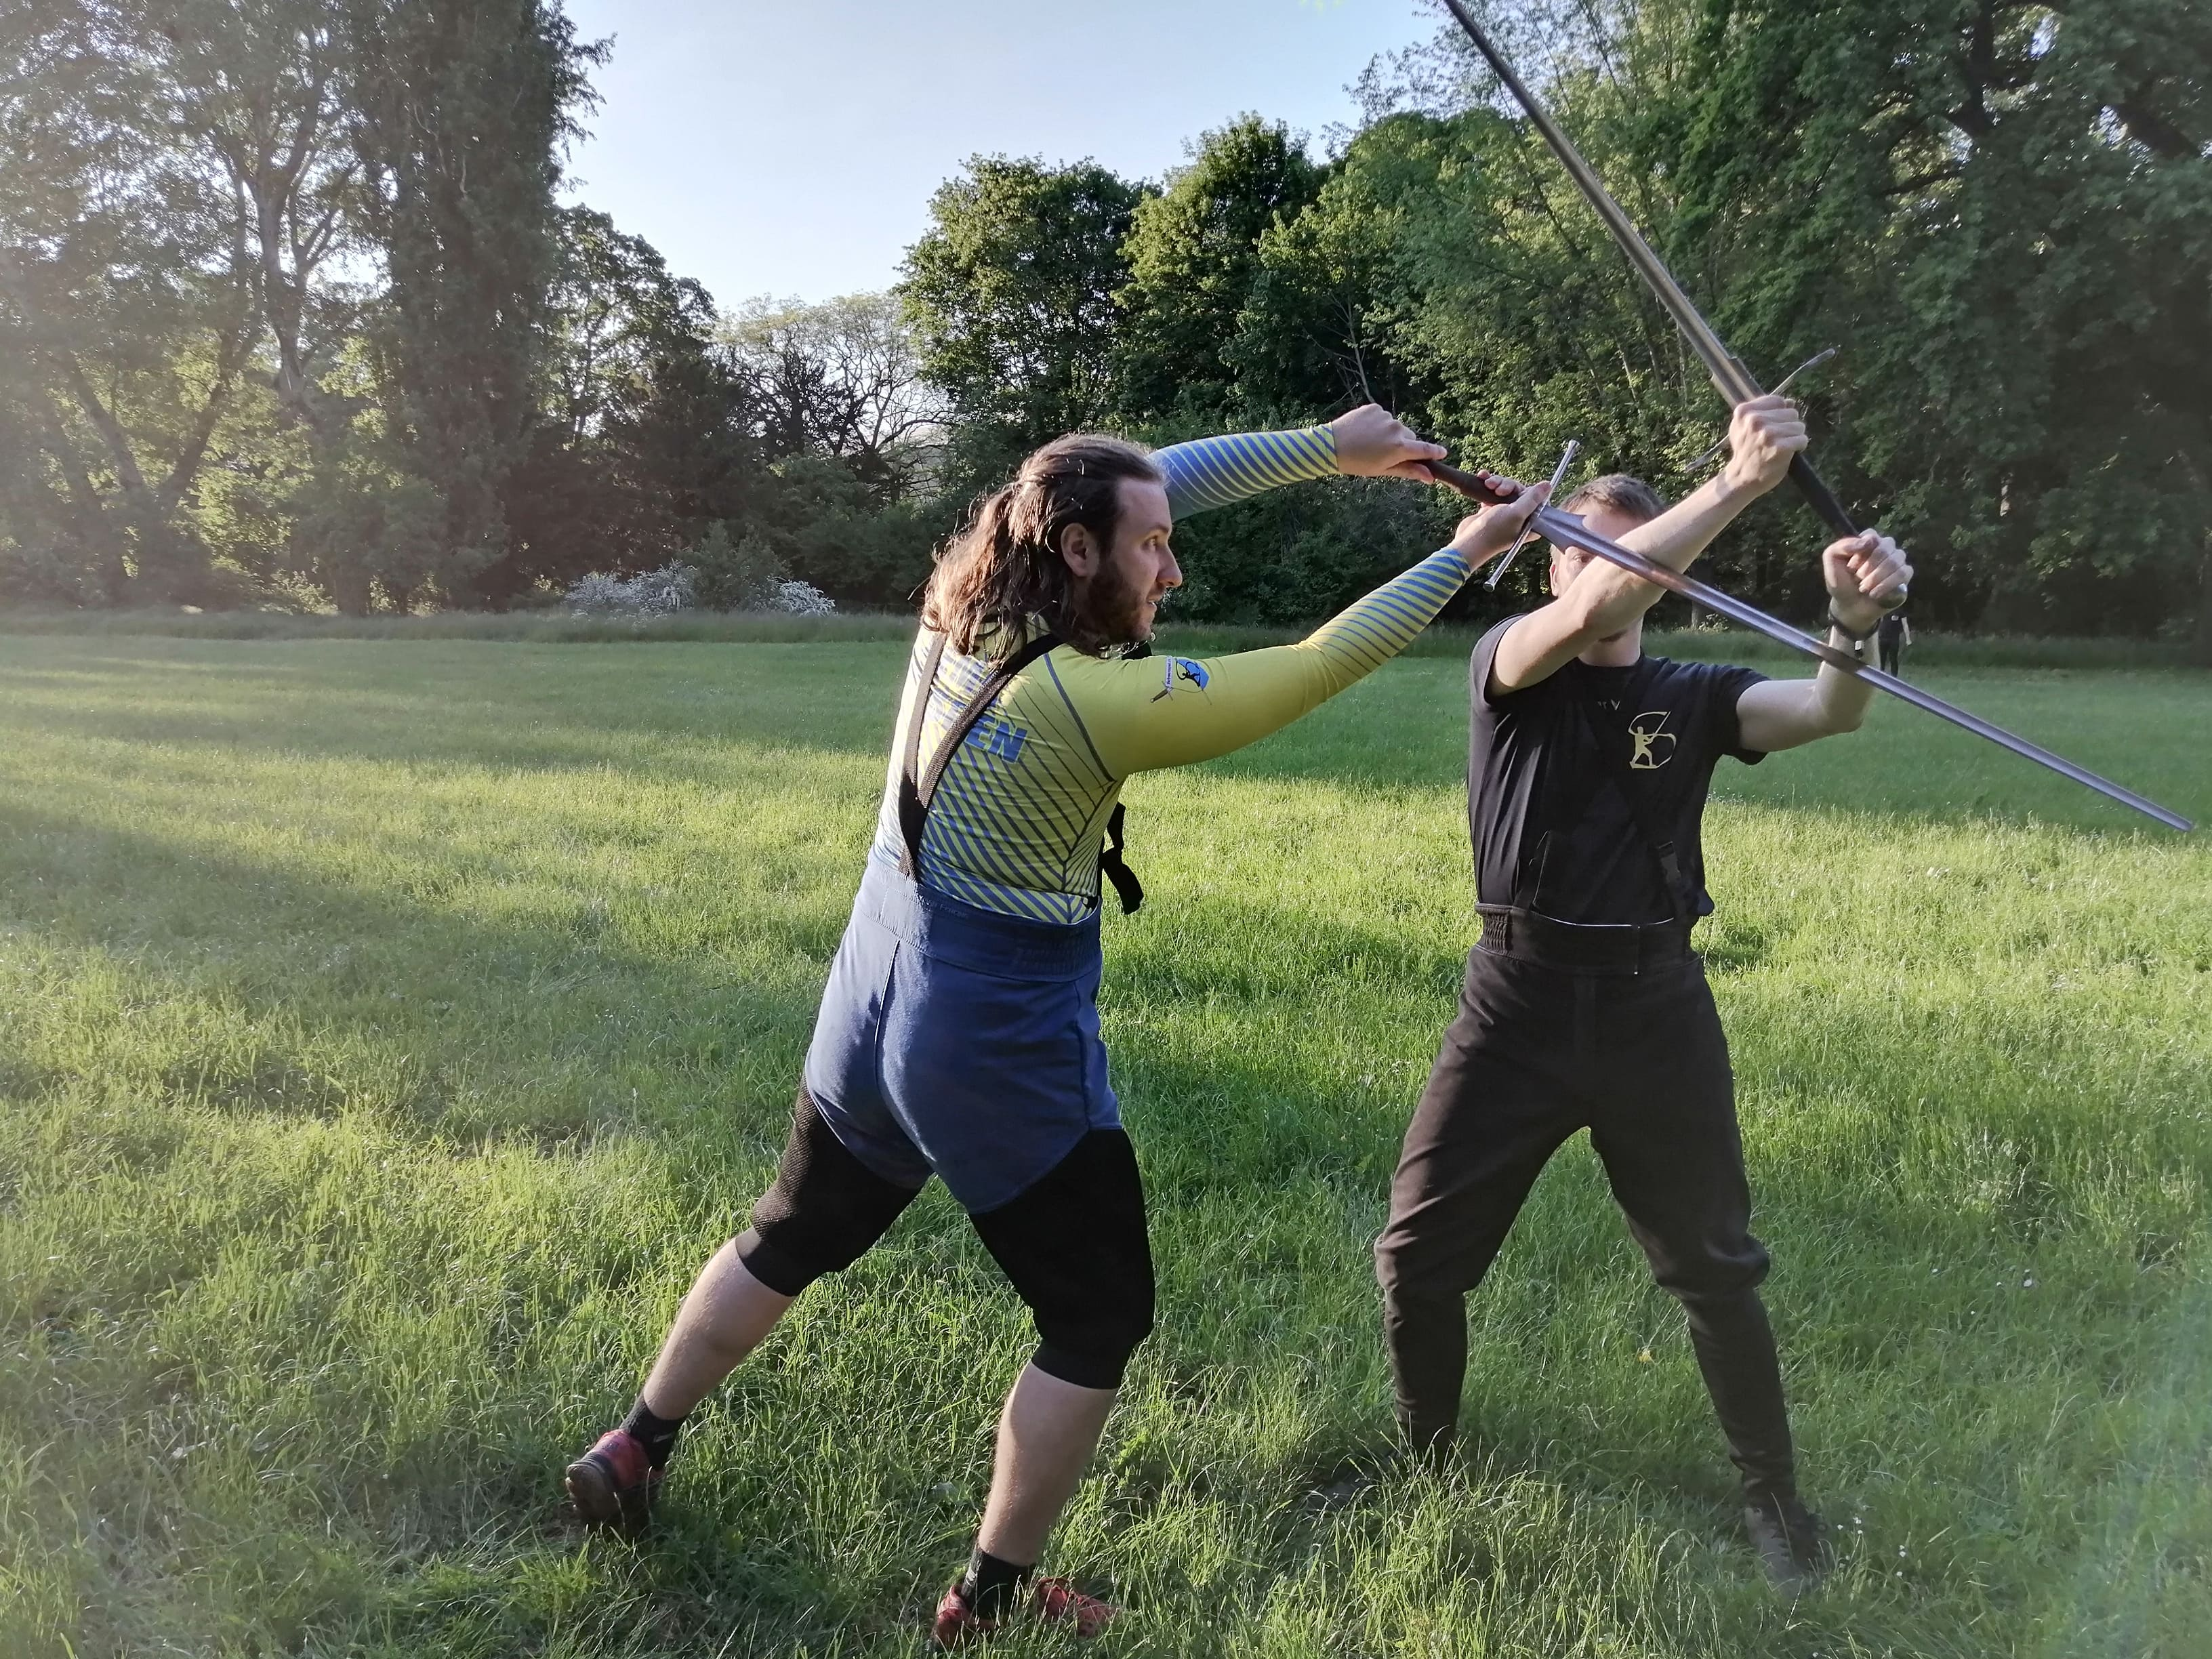
\includegraphics[width=\linewidth]{Schnitt4.jpg}
\endminipage
\end{figure}

\FloatBarrier

\newpage

\subsection{Erschließen eines Fechtstücks} 

Gemäß Maxime II ist ein jeder angehalten eine persönliche Interpretationen der Lehren Liechtenauers zu finden. Um diesen Findungsprozess ein wenig Struktur zu verleihen und einige Denkanstöße zu geben sei nachfolgend ein Vorschlag zur grundlegenden Strukturierung einer Interpretation vorgestellt, so wie sie auch im Training von Schwertspiel genutzt wird. Des Weiteren befindet sich im Anhang das Interpretationskonzept nach Thore Wilkens, an welches sich auch dieses Konzept anlehnt.

\subsubsection*{I.Ursache}

Beschreibt die Ausgangsituation: Welche Hut nehmen die Fechtenden ein und warum? Das Warum sollte in der Gruppe erläutert werden.

\subsubsection*{II.Auslöser}
Beschreibt den entscheidenden Moment, der die Ausführung des Stückes initiiert. Dieser sollte in der Gruppe besprochen werden, da dieser Auslöser später in Übungen genau erschlossen werden soll.

\subsubsection*{III.Ausführung}

Beschreibt die eigentliche Ausführung des Stücks: Diese soll in der Gruppe anhand der fechterischen Grundprinzipien ausführlich besprochen werden. Dies geschieht anhand von „Show and Tell“ durch die Fechter:innen im Dialog mit dem:der Trainer:in. Diese:r wirft das Augenmerk auf Mensur, Beinarbeit, Schwerthaltung und auf Beachtung der fechterischen Grundprinzipien.
 \\
 \\
 Schließlich wird die gefundene Interpretation noch einmal von den Trainer:innen vorgeführt. Anschließend haben die Fechter:innen in den folgenden Trainingseinheiten die Möglichkeit ihre persönliche Interpretation zu finden und zu festigen. Der Fokus der Übungen sollte Anfangs mehr auf dem Konditionieren des Auslösers liegen. Statische Übungen können dann genutzt werden bis alle Fechter:innen eine saubere Ausführung beherrschen. Anschließend wird der Auslöser in dynamischen Übungen wieder in den Fokus gesetzt. Schließlich kann das Fechtstück in offeneren dynamischen Übungen zusammen mit anderen Stücken in einen größeren Kontext gesetzt werden.

\newpage
\null
\thispagestyle{empty}
\newpage

\section{Fechtkanon}

Der nachfolgende Kanon ist eine Auswahl an Fechtstücken verschiedener Quellen. Diese wurden zu Themenschwerpunkten zusammengestellt, um an ihnen beispielhaft verschiedene fechterische Grundprinzipien zu erläutern. Die einzelnen Lektionen sind so angelegt, dass sie nicht auf einander aufbauen müssen. Man kann also die Kapitel in beliebiger Reihenfolge durchlaufen. Jedes Kapitel beginnt mit einem kurzen Einleitungstext, wechler die Schwerpunkte der Lektion kurz erläutert und Schlagworte nennt, die in der Lektion behandelt werden. Anschließend folgen die Fechtstücke der Lektion. Dabei befindet sich zunächst ein zweispaltiger Text, welcher links die Transkription (also die Übertragung der sprachlichen Ausdrücke der Originalquelle in moderne Schrift) und rechts eine Übersetzung (also eine syntaktische Übertragung in neuhochdeutsche Sprache) enthält. Auf der darauffolgenden Seite befinden sich Leerzeilen für eigene Notizen. Dies soll es ermöglichen, die eigene Interpretation möglichst nah an einer originalen Quelle zu orientieren.

\clearpage

\subsection{Mensur und Blößen}

\begin{center}
\resizebox{\textwidth}{!}{\textbf{Eintritt ins Gefecht  | Mensurgefühl | Mensurwechsel | Vor/Nach/Indes | Eigenschutz | Blößen}}
\end{center}
Der Fokus in diesem Teil liegt vor allem auf die dem Abschätzen von Distanzen, sowohl örtlich als auch zeitlich, im Großen wie im Kleinen. Die Fechtenden lernen über den Oberhau, beginnend in der weiten Mensur, wie sie phasenlos in ein Gefecht eintreten können und mögliche mentale Hindernisse überwinden. Dadurch können sie im Selbstversuch erfahren, bei welcher Mensur welche Mittel zum Treffen notwendig sind.
\\
\\
Anschließend wird mit dem \textbf{Nachreisen} ein Beispiel gegeben, wie ein fehlerhaftes Mensurverhalten des:der Gegner:in zum eigenen Vorteil genutzt werden kann. Dabei wird auch das Konzept der zeitlichen Abgrenzung durch Vor/Nach/Indes eingeführt und wiederholt. Es sollten mehrere Varianten des Nachreisens behandelt werden, um auch  explizit auf verschiedene Möglichkeiten des Eigenschutzes (Schwertbewegung/ Körperbewegung/ Beinarbeit) eingehen zu können.
\\
\\
Die Prinzipien des Eigenschutzes sollen weiterhin über das \textbf{Überlaufen} gefestigt werden. Speziell soll mit dem Überlaufen auf die Wichtigkeit des Kennens der eigenen sowie der gegnerischen Blößen eingegangen werden.
\\
\\
Um das bisher Gelernte in einen dynamischen Kontext zu setzten soll der \textbf{Scheitelhau} als Meisterhau genutzt werden. Alle in diesem Teil erlernten Prinzipien (richtiges Einschätzen der Mensur, Erkennen der Blößen des:der Gegner:in, Wissen um die eigenen Blößen, Durchlaufen verschiedener Prinzipien zum Eingeschutz) sind Grundlage für eine Gelungene Ausführung des Scheitelhaus.
\\
\\
Der Scheitelhau sollte mit einer darauffolgenden Versatzung gelehrt werden, da dies die Ausganssituation zum \textbf{Durchlaufen} bietet. Letzteres stellt den Eintritt in die Ringmensur dar. Gleichzeitig bleibt der Scheitelhau nicht als alleinstehendes Stück unkommentiert, denn den Fechtenden wird demonstriert, dass sich durch jede Aktion neue Stücke ergeben.
\\
\\
Damit können den Fechtenden in dieser Lektion anschaulich verschiedene wichtige Grundprinzipien gezeigt werden. Gleichzeitig wird den Fechtenden ein kleiner Katalog an Möglichkeiten im Spiel mit Mensur und Tempo in die Hand gegeben.
\\
\\
\textbf{Stücke und Schwerpunkte}

\begin{itemize}
    \item Nachreisen
    \item Überlaufen
    \item Scheitelhau
    \item Durchlaufen
\end{itemize}

\newpage

\subsubsection[Nachreisen]{Nachreisen\footnote{\hspace*{0.5ex}Rom, Biblioteca dell'Accademia Nazionale dei Lincei e Corsiniana, Cod. 1449 (Standortnummer 44 A 8), fol. 27v-28r, Transkription und Übersetzung: Dierk Hagedorn.}}

\begin{longtable}{p{6.25cm}p{6.25cm}}
\textbf{\textcolor{red}{ Das ist der text vnd die glos von dem nachraisen}}
&
\textbf{\textcolor{red}{Das Nachreisen}}
\\
\\
\textcolor{red}{Nachraisen lere zwifach oder schneid in die were Zwaÿ eüsserw mÿnne Der arbait dar nach begÿnne vnd prüf die gefert Ob sÿ sind waich oder hert}
&
\textcolor{red}{Lern das Nachreisen zweifach oder schneide in die Waffe. Trachte nach zwei Äußeren und beginn entsprechend deine Arbeit. Prüf, ob die Angriffe weich oder hart sind.}
\\
\\
| Glosa | Merck der nachraisen ist vil | vnd manigerlaÿ | vnd gehört zw treiben auß häwen | vnd aus stichen mit grosser fürsichtigkait gegen den vechterñ die da aus freÿem | vnd langen häwen fechten | vnd sünst von rechter kunst des swertz nicht wollen halden \textasciitilde 
&
Das Nachreisen ist vielseitig und von unterschiedlicher Art. Es wird sowohl aus Hieben als auch aus Stichen mit großer Umsicht gegen solche Fechter ausgeführt, die mit freien und ausgreifenden Hieben fechten und ohnehin von der richtigen Kunst des Schwertes nichts halten.
\\
\\
\textbf{\textcolor{red}{Das nachraisen treib also}}
&
\textbf{\textcolor{red}{Führ das Nachreisen folgendermaßen aus:}}
\\
\\
| Wenn dw mit dem zw° fechten zw° im ku\textasciitilde pst | So stee mit dem lincken fuess vor in der hu°t vom tag | vnd sich gar eben was er gegen dir vicht | Hawt er dir oben lanck ein so wart das er dich mit dem haw nicht erlang | Vnd merck die weil sein swert mit dem haw vndersich gee gegñ der erden | So spring zu° mit dem rechtñ füeß | vnd haw Im oben ein zw° dem kopff | ee wenn er mit dem swert wider auff kumpt | So ist er geschlagen \textasciitilde 
&
Wenn du im Zufechten zu ihm kommst, steh mit dem linken Fuß vor in der Hut vom Tag und beobachte genau, was er gegen dich unternehmen will. Schlägt er von oben lang zu dir, gib acht, daß er dich mit dem Hieb nicht erreicht. In dem Moment, da sein Schwert mit dem Hieb nach unten zu Boden weist, spring mit dem rechten Fuß vor, und schlag ihm oben zum Kopf, bevor er mit dem Schwert erneut hochkommt. So ist er geschlagen.
\end{longtable}





\newpage

\begin{center}
    \minisec{Notizen}
    \liniert[1cm]{18}
\end{center}

\newpage

\begin{longtable}{p{6.25cm}p{6.25cm}}
\textbf{\textcolor{red}{Das hernach geschriben stuck das haist die äussere mÿnn}}
&
\textbf{\textcolor{red}{Trachte nach den Äußeren.}}
\\
\\
| Merck | wenn er sich verhaut | vnd dw Im nach raistest mit dem haw zw° der plöss | vert er denn pald auff mit dem swert vñ kumpt dir vnden an dein swert | So pleib starck dar auff | Hebt er denn mit dem swert dein swert fast über sich | So spri\textasciitilde g mit dem lincken fuess hinder seinen rechten vnd slach | Im mit der twer oder f sünst zw° dem kopff seiner rechtñ seitten | vnd arbait pald wider vmb zw° seiner lincken seitten mit dem duplirñ | oder sünst mit anderñ stucken | Dar nach als dw emphindest | ob er waich oder hert am swert ist \textasciitilde \textasciitilde 
&
Wenn er seinen Hieb verreißt, reis ihm mit einem Hieb zu einer Blöße nach. Wenn er sogleich mit dem Schwert hochfährt und unten an dein Schwert kommt, bleib stark darauf. Hebt er dann mit seinem Schwert das deine stark nach oben, spring mit dem linken Fuß hinter seinen rechten und schlag ihm mit dem Twerhau oder einem anderen Hieb auf seiner rechten Seite zum Kopf. Arbeite sofort erneut zu seiner Linken mit dem Duplieren oder einem anderen Stück, je nachdem, wie du spürst, ob er weich oder hart am Schwert ist.
\end{longtable}

\newpage

\begin{center}
    \minisec{Notizen}
    \liniert[1cm]{18}
\end{center}

\newpage

\subsubsection[Überlaufen]{Überlaufen\footnote{\hspace*{0.5ex}Rom, Biblioteca dell'Accademia Nazionale dei Lincei e Corsiniana, Cod. 1449 (Standortnummer 44 A 8), fol. 29v-30r, Transkription und Übersetzung: Dierk Hagedorn.}}

\begin{longtable}{p{6.25cm}p{6.25cm}}
\textbf{\textcolor{red}{Hie merck den text vnd die glos von den vberlauffen}}
&
\textbf{\textcolor{red}{Das Überlaufen}}
\\
\\
\textcolor{red}{Wer vnden rempt Vber lauf den der wirt beschempt wenn es klitzt oben So sterck das ger ich loben Dein arbait mache oder herte druck zwifache}
&
\textcolor{red}{Überlauf den, der nach unten zielt; so wird er geschlagen. Wenn es oben klirrt, sei stark, das will ich loben. Mach deine Arbeit, oder drück kräftige Angriffe zweifach.}
\\
\\
| Glosa | merck das ist | wenn dw mit dem zu° vechten zw° Im kumpst haut er dir deñ vnden zw° den vnderñ plössen | das vor setz im nicht sunder haw Im oben starck ein zw° dem kopff | Oder haut er dir zw° mit vnder hawen | So merck ee wenn er mit dem vnderhaw auff kumpt | So scheüß Im den ort oben lanck ein zw° dem gesicht | oder der prust | vnd setz ÿm oben an so mag er dich vnden nicht erlangen | wenn alle oberñ an setzen prechñ | vnd ledigen die vnder | vert er denn auff | vnd pindt dir vnden an dein swert so pleib mit der langen schneid starck auff dem swert | vnd arbait behentlich zw der nagsten plöss oder lass in arbaitten | vnd kum dw | Inndes so trifestu In
&
Wenn du im Zufechten zu ihm kommst und er unten zu deinen unteren Blößen schlägt, dann versetz nicht, sondern schlag ihm oben kräftig zum Kopf. Oder, wenn er Unterhaue zu dir schlägt, gib acht, daß du, noch bevor er mit dem Unterhau hochkommt, ihm den Ort oben lang zum Gesicht oder zur Brust stichst, um ihm oben anzusetzen. So kann er dich unten nicht erreichen. Denn alle oberen Ansetzen brechen die unteren und befreien dich auch davon. Fährt er dann auf und bindet dir unten an dein Schwert, bleib mit der langen Schneide stark auf dem seinen und arbeite schnell zu seiner nächsten Blöße. Oder laß ihn angreifen, so daß du ihn »indes« triffst.
\end{longtable}

\newpage

\begin{center}
    \minisec{Notizen}
    \liniert[1cm]{18}
\end{center}

\newpage

\subsubsection[Scheitelhau]{Scheitelhau\footnote{\hspace*{0.5ex}Rom, Biblioteca dell'Accademia Nazionale dei Lincei e Corsiniana, Cod. 1449 (Standortnummer 44 A 8), fol. 24v-25r, Transkription und Übersetzung: Dierk Hagedorn.}}

\begin{longtable}{p{6.25cm}p{6.25cm}}
\textbf{\textcolor{red}{Hie hebt sich an der text vnd die glos von dem schaitelhaw}}
&
\textbf{\textcolor{red}{Der Scheitelhau}}
\\
\\
\textcolor{red}{De°m schaitlär dem antlutz ist gevär Mit seiner ker Der prust vast gever was von ÿm kumpt Die kron das ab nÿmpt Schneidt durch die kron So prichstu sy hart schon Die striche druck Mit schniten sy ab zuck}
&
\textcolor{red}{Der Scheitelhau ist dem Gesicht gefährlich. Mit seiner Umkehr stellt er eine große Gefahr für die Brust dar. Was von ihm kommt, fängt die Krone auf. Schneide durch die Krone, so hast du sie bereits kraftvoll gebrochen. Mach die Schläge mit Druck und zieh sie schnell mit Schnitten zurück}
\\
\\
| Glosa | Merck der schaitlär pricht die hu°t die da haist alber | vnd ist dar zu° dem antlütz | vnd der prust mit seiner ker gar gevardlich
&
Der Scheitelhau bricht die Hut Alber und ist weiterhin dem Gesicht und der Brust mit seiner Umkehr sehr gefährlich.
\\
\\
\textbf{\textcolor{red}{Den treib also}}
&
\textbf{\textcolor{red}{Er wird folgendermaßen ausgeführt:}}
\\
\\
| Wenn dw mit dem zu° vechten zw° ÿm kumpst legt er sich denn gegen dir in die hu°t alber | So setz den lincken fuess vor vnd halt dein swert an deiner rechten achsel Inn der hu°t | vnd spring zw° Im | vnd haw mit der langen schneid starck von oben nider Im zu° dem kopff | Vor setzt er denn haw das sein ort | vnd das ain gehultz paide übersich stenn das selb haist die kron | So beleib hoch mit den armen | vnd heb mit der lincken hant deinen swertz knopf vber sich | vnd senck im den ort vber sein gehültz zw der prust | Vert er denn auff mit dem swert | vnd stost dir den ort mit dem gehültz vber sich | So wind dein swert vnder seiner kron durch mit dem schnit in sein arm\textasciitilde  | vnd druck | Also ist die kron wider geprochen | vnd mit dem drucken | So schneid vast In die arm\textasciitilde  | vnd zeuch dich mit dem schnit ab
&
Wenn du im Zufechten zu ihm kommst und er sich vor dir in die Hut Alber begibt, so setz den linken Fuß vor und halt dein Schwert an der rechten Schulter in der Hut. Spring auf ihn zu und schlag ihm mit der langen Schneide kräftig von oben herab auf den Kopf. Wenn er den Hieb so versetzt, daß sowohl sein Ort als auch die eine Hälfte des Gehilzes nach oben zeigen, nennt man dies die Krone. Behalt die Arme oben und heb mit der linken Hand deinen Knauf nach oben und senk den Ort über seinem Gehilz zur Brust hin ab. Wenn er dann mit dem Schwert auffährt und dir den Ort mit dem Gehilz nach oben stößt, winde dein Schwert mit einem Schnitt in seine Arme unter seiner Krone durch und drück. So ist die Krone gebrochen. Schneide ihm im Wegdrücken kräftig in die Arme und zieh dich mit einem Schnitt ab.
\end{longtable}

\newpage

\begin{center}
    \minisec{Notizen}
    \liniert[1cm]{18}
\end{center}

\newpage

\subsubsection[Durchlaufen]{Durchlaufen\footnote{\hspace*{0.5ex}Rom, Biblioteca dell'Accademia Nazionale dei Lincei e Corsiniana, Cod. 1449 (Standortnummer 44 A 8), fol. 32r-32v, Transkription und Übersetzung: Dierk Hagedorn.}}

\begin{longtable}{p{6.25cm}p{6.25cm}}
\textbf{\textcolor{red}{Hie merck den text vnd die glos von den durchlauffen vnd von den ringen Im swert}}
&
\textbf{\textcolor{red}{Das Durchlaufen und das Ringen am Schwert}}
\\
\\
\textcolor{red}{Durchlauf lass hangen Mit dem knopf greif wiltu rangen wer gegen dir sterck durchlaüf do mit merck}
&
\textcolor{red}{Lauf durch. Laß hängen. Greif mit dem Knauf, wenn du ringen willst. Beachte, demjenigen durchzulaufen, der stark gegen dich ist.}
\\
\\
| Glosa | merck  die durchlauffen | vnd die ringñ sind zwaierlaÿ Im swert | wenn die durchlauffen das sind die leibt ringen | So sind denn dar nach die arm\textasciitilde  ringen | vnd die gehörent zw° treiben gegen den vechterñ | die do gerñ ein lauffent \textasciitilde 
&
Es gibt zweierlei Durchlaufen und Ringen am Schwert. Denn das Durchlaufen ist gleichbedeutend mit dem Leibringen. Außerdem gibt es das Armringen, welches gegen Fechter angewandt wird, die gerne einlaufen.
\\
\\
\textbf{\textcolor{red}{Die durchlauffen die treib des ersten also}}
&
\textbf{\textcolor{red}{Führ das Durchlaufen fürs erste folgendermaßen aus}}
\\
\\
| Merck | wenn er dir ein laufft | vnd vert hoch auff mit den armen | vnd wil dich oben mit sterck vber dringen | So var auch auff mit den armen | vnd halt dein swert mit der lincken hant peÿ dem knopff über deinem haubt | vnd lass die klingen vber deinen ruck hinden nider hangen | vnd lauff mit dem haubt durch die arm\textasciitilde  gegen sein° rechtñ seitten | vnd spring mit dem rechtñ fuess hinder sein rechtñ | vnd mit dem sprung so var Im mit dem rechtñ arm\textasciitilde  gegen seiner lincken seitten vorñ wol vmb den leip | vnd vass In also auff dein rechte hüff | vnd würff In für dich hinden auff sein kopff \textasciitilde 
&
Wenn er dir einläuft und die Arme hochreißt, um oben mit Kraft auf dich zu drängen, reiß ebenfalls die Arme hoch. Halt dein Schwert mit der linken Hand am Knauf über deinem Kopf und laß die Klinge hinten über deinen Rücken nach unten hängen. Lauf mit dem Kopf durch die Arme zu seiner Rechten. Spring mit dem rechten Fuß hinter seinen rechten und greif ihm im Sprung mit dem rechten Arm zu seiner linken Seite vorne weit um den Körper. Zieh ihn auf diese Weise auf deine rechte Hüfte und wirf ihn mit dem Hinterkopf vor dich.
\end{longtable}

\newpage

\begin{center}
    \minisec{Notizen}
    \liniert[1cm]{18}
\end{center}

\newpage

\subsection{Bindung I}\label{Bindung1}

\begin{center}
\resizebox{\textwidth}{!}{\textbf{Fühlen am Schwert | Anhand Bindungsstärke Technik adaptieren | Wechsel der Bindungsstärke}}
\end{center}
Diese Lektion befasst sich mit dem Aufbau einer Bindung und den sich daraus ergebenden Möglichkeiten. Dazu sollen zuerst anhand einer \textbf{einfachen Versatzung gegen Oberhäue} die Grundprinzipien zum Eigenschutz gezeigt bzw. wiederholt werden.
\\
\\
Anschließend sollen aus der einer neutralen Position durch verschiedene Übung zum Erfühlen verschiedene Prinzipien über die Arten von Bindungen gefunden werden (Hart am Band – Leichter in der Stärke, Weich leichter in der Schwäche usw.). Ausgehend davon wird über das \textbf{Einwinden / Auswinden} gezeigt, wie bewusst über die Art und den Ort der Bindung Druck zum gegenüber aufgebaut werden kann. Dabei ist besonders herauszustellen, wie die Stärke am Band das Verhalten in der Bindung beeinflusst.
\\
\\
Dies kann anschließend über das \textbf{Mutieren} erweitert werden. Weiterhin kann über das \textbf{Duplieren} gezeigt werden, wie man falsches oder ungenaues Anbinden des Gegenübers zum eigenen Vorteil nutzen kann.
\\
\\
Schließlich bietet der \textbf{Schielhau} aus der Bindung eine Anwendung eines Meisterhaues aus der Bindung, als auch einen Ausblick auf weitere Lektionen.
\\
\\
Diese Lektion gibt den Fechtenden die Fähigkeit aus dem Erfühlen einer Bindung eine Fechtsituation lesen zu können und gibt ihnen einen beispielhaften Katalog an Handlungsmöglichkeiten, für die Bindung. Es wird außerdem vermittelt, dass Kraft immer Maßvoll eingesetzt werden sollte, um dem Gegenüber keine ungewollten Möglichkeiten zu eröffnen.
\\
\\
Stücke und Schwerpunkte

\begin{itemize}
    \item Einwinden
    \item Auswinden
    \item Mutieren
    \item Duplieren
    \item Schielhau aus der Bindung
\end{itemize}

\hspace{0.5cm}

\begin{itemize}
    \item Gedeckte Bindung/Eigenschutz, Fühlen
    \item das schwache und das starke Band
    \item zu starkes Versetzen
\end{itemize}

\newpage
\null
\thispagestyle{empty}
\newpage

\subsubsection[Ein- und Auswinden von rechts]{Ein- und Auswinden von rechts\footnote{\hspace*{0.5ex}Rom, Biblioteca dell'Accademia Nazionale dei Lincei e Corsiniana, Cod. 1449 (Standortnummer 44 A 8), fol. 37v-38r, Transkription und Übersetzung: Dierk Hagedorn.}}

\begin{longtable}{p{6.25cm}p{6.25cm}}
\textbf{\textcolor{red}{Hie merck eben wie du aus den oberñ zwaien hengen das ist aus dem ochsen von der rechten seitten vnd von der linken seitten solt treiben vier winden}}
&
\textbf{\textcolor{red}{Wie du aus den oberen zwei Hängen, also aus dem Ochs, von rechts und links vier Winden ausführen sollst}}
\\
\\
| Dÿe ersten tzwaÿ winden aus dem ochsen allai\textasciitilde  von der rechten seitten die treib also | Weñ dw mit dem zw° vechten zu° Im kumpst | So stee mit dem lincken fuess vor | vnd halt dein swert zw deiner rechten seittñ fur dem haubt In dem ochsen | Hawt er dir denn oben ein von seiner rechten seitten | So wind auff dein lincke seittñ gegen seine\textasciitilde m haw die kurtz schneÿd an sein swert aber in den ochsen | vnd stich Im oben ein zw dem gesicht das ist ein winden 
&
Mach die ersten zwei Winden aus dem rechten Ochs folgendermaßen: Wenn du im Zufechten zu ihm gehst, steh mit dem linken Fuß vor und halt dein Schwert an deiner rechten Seite vor dem Kopf im Ochs. Schlägt er dann oben von seiner rechten Seite, winde auf deine linke Seite, seinem Hieb entgegen erneut in den Ochs, die kurze Schneide an sein Schwert. Stich ihm oben zum Gesicht. Dies ist ein Winden.
\\
\\
Merck | Vor setzt er den stich mit sterck | vnd dringt dir das swert auff die seitten so pleib am swert | vnd wind wider auf dein rechte seitten ober Inn den ochsen | vnd stich Im oben ein zw dem gesicht das sein die zwaÿ winden am swert aus dem ainen oberñ hengen von der rechten seitten \textasciitilde 
&
Versetzt er den Stich mit Stärke und drückt dir das Schwert zur Seite, so bleib am Schwert, winde wieder zu deiner Rechten oben in den Ochs und stich ihm oben zum Gesicht. Dies sind die zwei Winden am Schwert aus dem einem oberen Hängen auf der rechten Seite.
\end{longtable}

\newpage

\begin{center}
    \minisec{Notizen}
    \liniert[1cm]{18}
\end{center}

\newpage

\subsubsection[Ein- und Auswinden von links]{Ein- und Auswinden von links\footnote{\hspace*{0.5ex}Rom, Biblioteca dell'Accademia Nazionale dei Lincei e Corsiniana, Cod. 1449 (Standortnummer 44 A 8), fol. 38r, Transkription und Übersetzung: Dierk Hagedorn.}}

\begin{longtable}{p{6.25cm}p{6.25cm}}
\textbf{\textcolor{red}{Hye merck das sind die anderñ zwaÿ winden aus dem ochsen von der lincken seitten die treib Also}}
&
\textbf{\textcolor{red}{Dies sind die anderen zwei Winden aus dem linken Ochs. Führ sie folgendermaßen aus}}
\\
\\
| wenn dw mit dem zu° vechten zu° ÿm kumpst | So stee von dein° lincken seitten In dem ochsen haut er dir denn oben ein von seiner lincken seitten | So wind gegen seinem haw auff dein rechte seittñ die lang schneid an das swert | vñ stich Im oben ein zw dem gesicht das ist ein winden Merck | Vor setzt er den stich | vnd druckt dein swert auff die seittñ | So pleib am swert | vnd wind auff dein lincke seitten aber in den ochsen die lang schneid an sein swert | vnd stich ÿm oben ein zw dem gesicht | Das sind die vier winden aus den oberñ zwaÿen hengen von der lincken vnd von der rechtñ seittñ
&
Wenn du im Zufechten zu ihm gehst, steh im linken Ochs. Schlägt er dann oben von seiner  linken Seite, winde, seinem Hieb entgegen, auf deine rechte Seite die lange Schneide ans Schwert und stich ihm oben zum Gesicht. Dies ist ein Winden. Versetzt er den Stich und drückt dein Schwert zur Seite, so bleib am Schwert, winde zu deiner Linken erneut in den Ochs, die lange Schneide an sein Schwert, und stich ihm oben zum Gesicht. Dies sind die vier Winden am Schwert aus den oberen zwei Hängen auf der linken und rechten Seite.
\end{longtable}

\newpage

\begin{center}
    \minisec{Notizen}
    \liniert[1cm]{18}
\end{center}

\newpage

\subsubsection[Mutieren]{Mutieren\footnote{\hspace*{0.5ex}Rom, Biblioteca dell'Accademia Nazionale dei Lincei e Corsiniana, Cod. 1449 (Standortnummer 44 A 8), fol. 16v, Transkription und Übersetzung: Dierk Hagedorn.}}

\begin{longtable}{p{6.25cm}p{6.25cm}}
\textbf{\textcolor{red}{Hie merck wie man das mutirñ treibñ solt zw paiden seiten}}
&
\textbf{\textcolor{red}{Das Mutieren auf beiden Seiten}}
\\
\\
| Merck | wenn dw ym von deiner rechten achsel oben starck ein haust zw dem kopff | vor setzt er vnd ist waich am swert | So wind auff dein lincke seitten die kurtz schneid an sein swert | vnd var wol auff mit den armen | vnd var ÿm mit deiner swertz klingen oben vber sein swert | vnd stich ÿm zu der underñ plöss
&
Wenn du von deiner rechten Schulter kräftig oben zu seinem Kopf schlägst, was er versetzt und weich am Schwert ist, so winde die kurze Schneide an seinem Schwert auf deine linke Seite und fahr dabei angemessen mit den Armen auf. Fahr ihm mit deiner Klinge oben über sein Schwert und stich ihm zur unteren Blöße.
\\
\\
\textbf{\textcolor{red}{Ein anders}}
&
\textbf{\textcolor{red}{Ein weiteres Stück}}
\\
\\
| Merck | wenn du ÿm von deiner lincken seitten oben ein haust zu° dem kopff vor setzt er | vnd ist waich am swert  | So var auff mit den armen | vnd heng ÿm den ort oben über sein swert | vnd stich in zu° der vnderñ plöß | Also magstu die tzwai stuck treiben aus allen häwen | Dar nach als dw emphindest swech vnd sterck am swert
&
Wenn du ihm von deiner linken Seite oben zum Kopf schlägst, was er versetzt und weich am Schwert ist, so fahr mit den Armen auf, häng ihm den Ort oben über sein Schwert und stich zur unteren Blöße.
Diese zwei Stücke kannst du aus allen Hieben heraus anwenden, je nachdem, wie du Schwäche und Stärke am Schwert spürst.
\end{longtable}

\newpage

\begin{center}
    \minisec{Notizen}
    \liniert[1cm]{18}
\end{center}

\newpage

\subsubsection[Duplieren]{Duplieren\footnote{\hspace*{0.5ex}Rom, Biblioteca dell'Accademia Nazionale dei Lincei e Corsiniana, Cod. 1449 (Standortnummer 44 A 8), fol. 16r, Transkription und Übersetzung: Dierk Hagedorn.}}

\begin{longtable}{p{6.25cm}p{6.25cm}}
\textbf{\textcolor{red}{Hye merck wie du das duplierñ treiben solt zw paiden seitten}}
&
\textbf{\textcolor{red}{Das Duplieren auf beiden Seiten}}
\\
\\
| Merck wenn er dir oben zu° haut von seiner rechten achsal | So haw auch von deiner rechten mit ym geleich oben starck ein zu° dem kopff | ver setzt er | vnd beleibt starck am swert | So var Indes auff mit den armen | vnd stos mit der lincken hant dein swertz knopff vnder deinen rechten arm\textasciitilde  | vnd slach ÿn mit der langen schneid pis aus gekreutzten arm\textasciitilde  hinder seiner swertz klingen auff den kopf \textasciitilde 
&
Wenn er oben von seiner rechten Schulter zu dir schlägt, schlag ihm ebenfalls von deiner Rechten gleichzeitig oben kraftvoll zum Kopf. Wenn er versetzt und stark am Schwert bleibt, fahr »indes« mit den Armen auf und stoß mit der linken Hand den Knauf deines Schwertes unter deinen rechten Arm und schlag ihm mit der langen Schneide und mit gekreuzten Armen hinter seiner Schwertklinge auf den Kopf.
\\
\\
\textbf{\textcolor{red}{Ein anders}}
&
\textbf{\textcolor{red}{Ein weiteres Stück}}
\\
\\
| Merck haut er dir von seiner lincken achsal mit der langen schneid oben ein zw dem kopff vnd tue ym also | wider bleibt er denn starck am swert | So var pald auff mit den armen | vnd slach yn hinder seiner swertz klingen mit der kurtzen schneid auff den kopff
&
Schlägt er mit der langen Schneide von seiner linken Schulter oben zu deinem Kopf, so tu es ihm gleich. Bleibt er dann stark am Schwert, fahr sofort mit den Armen auf und schlag ihm hinter seiner Schwertklinge mit der kurzen Schneide auf den Kopf.
\end{longtable}

\newpage

\begin{center}
    \minisec{Notizen}
    \liniert[1cm]{18}
\end{center}

\newpage

\subsubsection[Schielhau]{Schielhau\footnote{\hspace*{0.5ex}Rom, Biblioteca dell'Accademia Nazionale dei Lincei e Corsiniana, Cod. 1449 (Standortnummer 44 A 8), fol. 23r-24v, Transkription und Übersetzung: Dierk Hagedorn.}}

\begin{longtable}{p{6.25cm}p{6.25cm}}
\textbf{\textcolor{red}{Hie hebt sich an der schilhaw mit seinen stucken}}
&
\textbf{\textcolor{red}{Der Schielhau mit seinen Stücken}}
\\
\\
\textcolor{red}{Schilär ein pricht was püffel schlecht oder sticht wer wechsel draut Schilär dar aus In beraupt}
&
\textcolor{red}{Der Schielhau bricht, was ein Büffel schlägt oder sticht. Wer droht durchzuwechseln, wird mit dem Schielhau daran gehindert.}
\\
\\
| Glosa | Merck der schilär pricht die hu°t die do haist der pflugk | vnd ist ein seltzam | gu°t eñhaft haw | wenn er pricht mit gewalt ein Inn haw | vnd in stichen | vnd get zu° mit verkärtem swert | Dar vmb sind viel maister des swertz die von dem haw nicht wissen ze sagen \textasciitilde 
&
Der Schielhau bricht die Hut Pflug. Er ist ein außergewöhnlich wirksamer Hieb, denn er bricht mit Macht in Hiebe und Stiche ein. Er wird mit verdrehtem Schwert ausgeführt. Deshalb gibt es viele Meister des Schwertes, die diesen Hieb nicht kennen.
\\
\\
\textbf{\textcolor{red}{Hie merck wie man den schilär hauen sol}}
&
\textbf{\textcolor{red}{Wie man den Schielhau schlagen soll}}
\\
\\
| Merck | wenn du mit dem zu° vechten zw° ym kumpst | So stee mit dem lincken fuess vor | vnd halt dein swert an deiner rechtñ achsel | hawt er dir denn oben ein zw° dem kopff | So ver wennt dein swert | vnd haw gegen seinem haw mit der kûrtzen schneid lanck aus gerackten armen ober vber sein swert Im zu° dem kopff | Ist er denn also gescheid | vnd verfelt mit dem haw deins swertz | vnd wil vnden durch wechselñ | So lass den ort mit dem haw fürsich lanck ein schiessen | So mag er vnden nicht durch wechseln
&
Wenn du im Zufechten zu ihm kommst, steh mit dem linken Fuß vor und halt dein Schwert an der rechten Schulter. Wenn er dann oben zu deinem Kopf schlägt, dreh dein Schwert und schlag mit der kurzen Schneide und lang ausgestreckten Armen gegen seinen Hieb und schlag ihm oben über sein Schwert zum Kopf.
Wenn er so geschickt ist, dem Hieb deines Schwertes auszuweichen, um unten durchzuwechseln, dann stoß den Ort aus dem Hieb heraus lang geradeaus. So kann er nicht unten durchwechseln.
\end{longtable}

\newpage 

\begin{center}
    \minisec{Notizen}
    \liniert[1cm]{18}
\end{center}

\newpage

\begin{longtable}{p{6.25cm}p{6.25cm}}
\textbf{\textcolor{red}{Das ist der text vnd die glos wie man mit dem schilär pricht den langen ort}}
&
\textbf{\textcolor{red}{Wie man mit dem Schielhau den Langort bricht}}
\\
\\
\textcolor{red}{Schül zw dem ort vnd nÿm den hals ane vorcht}
&
\textcolor{red}{Schiel auf den Ort und nimm furchtlos den Hals.}
\\
\\
| Glosa | Merck wenn du mit dem zü fechten zw° ÿm kumpst | Stet er denn gegen dir | vnd helt dir den langen ort gegen dem gesicht oder der prust | So halt dein swert an der rechten achsel | vnd schil mit dem gesicht zu° dem ort | vnd thu°e als dw ÿm dar zu° hauen wöllest | vnd haw starck mit dem schilär mit der kurtzen schneid an sein swert | vñ scheus ÿm den ort do mit lanck ein ze dem hals mit einem zw° tritt des rechten füess \textasciitilde 
&
Wenn du im Zufechten zu ihm kommst und er vor dir steht, indem er dir den Langort gegen Gesicht oder Brust hält, so halt dein Schwert an der rechten Schulter. Schiel mit den Augen zum Ort und tu so, als wollest du ihm dorthin schlagen. Schlag einen kräftigen Schielhau mit der kurzen Schneide an sein Schwert und stoß ihm dabei den Ort lang zum Hals, indem du einen Vorwärtsschritt mit dem rechten Fuß machst.
\\
\\
\textbf{\textcolor{red}{Das ist der text vnd die glos aber eins stucks aus dem schil haw}}
&
\textbf{\textcolor{red}{Ein weiteres Stück vom Schielhau}}
\\
\\
\textcolor{red}{Schil zw dem oberñ haupt hend wildw bedöberñ}
&
\textcolor{red}{Schiel nach oben zum Kopf, wenn du den Händen schaden willst.}
\\
\\
| Glosa | Merck das ist ein ander pruch | weñ er gegen dir stet in dem langen ort | So schil ÿm mit dem gesicht zw° dem haubt | vnd thu°e als du in dar auff wöllest sla schlachen | vnd schlach in auß dem schilhaw mit dem ort auff sein hend \textasciitilde 
&
Dies ist ein weiterer Bruch. Wenn er im Langort vor dir steht, schiel mit den Augen zum Kopf und tu so, als wollest du dorthin schlagen. Schlag ihm aber mit dem Schielhau den Ort auf die Hände.
\end{longtable}

\newpage 

\begin{center}
    \minisec{Notizen}
    \liniert[1cm]{18}
\end{center}

\newpage

\subsection{Unterhau und Untere Huten}\label{Unten}

\begin{center}
\resizebox{\textwidth}{!}{\textbf{Huten | Blößen | Untere Huten mit Anwendung | Mensurgefühl | Timing}}
\end{center}
Unterhäue und untere Huten finden im modernen HEMA mitunter wenig Beachtung. Daher sollen in dieser Lektion die Vorzüge und Besonderheiten der unteren Häue und Huten behandelt werden. Dazu wird zunächst der \textbf{Unterhau} aus den oberen Huten in verschiednene Kontexte gesetzt und dessen Vorzüge und Besonderheiten dargestellt.
\\
\\
Anschließend werden die verschiedenen \textbf{unteren Huten} und jeweils der daraus mögliche Gefechtseintritt und Stücke kurz dargestellt, um den Fechtenden Anwendungsmöglichkeiten für die unteren Huten aufzuzeigen.
\\
\\
Speziell soll hier das \textbf{Streichen} als defensiver Eintritt ins Gefecht herausgestellt werden, welches mit einem weiteren Unterhau fortgesetzt werden kann. Hierbei sei vor allem auf das Prinzip der Erhaltung des Bewegungsflusses verwiesen.
\\
\\
Weiterhin werden das \textbf{Abschneiden} und der \textbf{Unterschnitt} als Anwendungen aus den unteren Huten oder für Unterhäue dargestellt. Wobei speziel Vor/Indes und das rechzeitige Initiieren der Aktion behandelt werden soll.
\\
\\
Schließlich bildet der \textbf{Krumphau} aus der Schrankhut als Meisterhau aus den unteren Huten den Abschluss dieser Lektion.
\\
\\
Die Lektion gibt den Fechtenden die Möglichkeit das Gefecht aus einer unteren Hut zu führen, das heißt sie zeigt die Vor- und Nachteile der Huten und Häue auf, legt die Wichtigkeit von Huten, das Wissen um ihre Blößen und die daraus hervorgehenden Erwartung des Gegenübers, sowie die sich daraus ergebenden Möglichkeiten.
\\
\\
Stücke und Schwerpunkte:

\begin{itemize}
    \item Streichen
    \item Schnappen
    \item Krumphau aus der Schrankhut 
\end{itemize}

\hspace{0.5cm}

\begin{itemize}
    \item Unterhau
    \item Untere Huten
    \item Abschneiden
    \item Unterschnitt
\end{itemize}

\newpage
\null
\thispagestyle{empty}
\newpage

\subsubsection[Streichen]{Streichen\footnote{\hspace*{0.5ex}Paurenfeyndt, Andre: Ergrundung Ritterlicher Kunst der Fechterey, Wien 1516, S. 30, Transkription: Chidester, eigene Übersetzung}}

\begin{longtable}{p{6.25cm}p{6.25cm}}
\textbf{STUCK ym auftreichen[!]}
&
\textbf{Vom Aufstreichen}
\\
\\
Wan du leist yn der neben huet auf deiner lincken seiten, vud ainer haut auf dich ain oberhau von seiner rechten axel so streich von unden auf vast yn sein schwert mit der kurczen scneid, helt er starck wider und ist nit hoch mit den henden, so duplier czwischen dem man und seinem schwert ein, mit der kurczen schneid czu seinem lincken or
&
Wenn du in der Nebenhut auf deiner linken Seite stehst und Einer dir einen Oberhau von seiner rechten Seite schlägt, so streich von unten auf, gegen sein Schwert mit der kurzen Schneide. Hält er stark dagegen und hält er seine Händen nicht hoch, so duplier zwischen dem Mann und seinem Schwert mit der kurzen Schneide zu seinem linken Ohr.
\end{longtable}

\newpage

\begin{center}
    \minisec{Notizen}
    \liniert[1cm]{18}
\end{center}

\newpage

\subsubsection[Schnappen]{Schnappen\footnote{\hspace*{0.5ex}Rom, Biblioteca dell'Accademia Nazionale dei Lincei e Corsiniana, Cod. 1449 (Standortnummer 44 A 8), fol. 34v, Transkription und Übersetzung: Dierk Hagedorn.}}

\begin{longtable}{p{6.25cm}p{6.25cm}}
\textbf{\textcolor{red}{Aber ein anders}}
&
\textbf{\textcolor{red}{Ein weiteres Stück}}
\\
\\
| Wenn du zw° vichtest mit vnder häwen oder ligst in der hu°t alber | Velt er denn mit dem swert auff das dein nahent pey dem gehültz ee | wenn du do mit auff chumpst das sein ort zw° deiner rechten seitten auß (*) get | So var behendlich auff mit dem knopff vber sein swert vnd schlag in mit der langen schneid zw° dem kopf | Oder pint er dir auff das swert das sein ort zu° deiner lincken seitten | So var mit dem knopf vber sein swert | vnd slach In mit der kurtzen schneid zw° dem haupt das haist das schnappen \textasciitilde 
&
Wenn du im Zufechten mit einem Unterhau angreifst oder in der Hut Alber liegst und er dir mit dem Schwert auf das deine nahe dem Gehilz fällt, bevor du es noch erheben konntest, so daß sein Ort zu deiner Rechten zeigt, so fahr schnell mit dem Knauf über sein Schwert. Schlag ihm mit der langen Schneide zum Kopf. Bindet er dir aber auf das Schwert, so daß sein Ort zu deiner linken Seite zeigt, so fahr mit dem Knauf über sein Schwert und schlag ihm mit der kurzen Schneide zum Kopf.
Dies nennt sich Schnappen.
\end{longtable}

\newpage

\begin{center}
    \minisec{Notizen}
    \liniert[1cm]{18}
\end{center}
\newpage

\subsubsection[Krumphau / Krumphau aus der Schrankhut]{Krumphau / Krumphau aus der Schrankhut\footnote{\hspace*{0.5ex}Rom, Biblioteca dell'Accademia Nazionale dei Lincei e Corsiniana, Cod. 1449 (Standortnummer 44 A 8), fol. 16v-17v, Transkription und Übersetzung: Dierk Hagedorn.}}

\begin{longtable}{p{6.25cm}p{6.25cm}}
\textbf{\textcolor{red}{Das ist der text vnd die glos von dem krump haw mit seinen stucken}}
&
\textbf{\textcolor{red}{Der Krumphau}}
\\
\\
\textcolor{red}{krump auf behende wirff den ort auf die hende krump wer wol setzet Mit schritten vil häw letzet}
&
\textcolor{red}{Schlag den Krumphau geschickt, schleuder den Ort auf die Hände. Wer den Krumphau mit Schritten gut ausführen kann, kann viele Hiebe aufhalten und vergelten.}
\\
\\
| Merck der krump haw ist der vier vor setzen ains wider die vier hüten | wenn do mit pricht man die hüten | Die do haist der öchss | vnd auch der öber | vnd den vnder haw den treib also | wenn du mit dem zu° vechten zw° im kumpst stet er denn gegen dir | vnd helt sein swert für seinem haubt | In der hu°t des ochsens auff seiner lincken seitten | So setz den lincken fues vor | vnd halt dein swert an deiner rechten achsel in der hu°t | vnd spring mit dem rechten fuess wol auff dein rechte seitten gegen ÿm | vnd slach ÿn mit der langen schneid aus gekräutzten armen vber sein hend
&
Der Krumphau ist eines der vier Versetzen gegen die vier Huten. Mit ihm bricht man die Hut Ochs sowie Ober- und Unterhaue. Führ ihn folgendermaßen aus: Wenn du im Zufechten zu ihm kommst und er mit dem Schwert vor seinem Kopf in der Hut des linken Ochsen vor dir steht, so setz den linken Fuß vor und halt dein Schwert an der rechten Schulter in der Hut. Spring mit dem rechten Fuß entschieden zu deiner rechten Seite auf ihn zu. Schlag ihm mit der langen Schneide mit gekreuzten Armen über seine Hände.
\end{longtable}

\newpage

\begin{center}
    \minisec{Notizen}
    \liniert[1cm]{18}
\end{center}

\newpage

\begin{longtable}{p{6.25cm}p{6.25cm}}
\textbf{\textcolor{red}{Ein anders}}
&
\textbf{\textcolor{red}{Ein weiteres Stück}}
\\
\\
| Merck den krump haw magstu auch treiben aus der schranck hu°t von paiden seittñ | vnd in die hu°t schick dich also | wenn dw mit dem zu° vechten zw° ÿm kumpst | So ste mit dem lincken fuess vor | vnd halt dein swert mit dem ort neben deiner rechten seitten auff der erden das die lang schneid oben seÿ | vnd gib dich plöß mit der lincken seitten haut er dir denn zw° der plöss | So spring aus dem haw gegen ÿm mit dem rechten fuëss wol auff dein rechte seitten | vnd slach ÿn mit gekräutzten henden aus der langen schneid mit dem ort auff sein hend
&
Du kannst den Krumphau auch aus der Schrankhut von beiden Seiten ausführen. Stell dich folgendermaßen in diese Hut: Wenn du im Zufechten zu ihm kommst, steh mit dem linken Fuß vor und halt dein Schwert mit dem Ort neben deiner rechten Seite auf die Erde, so daß die lange Schneide nach oben zeigt. Gib dir so auf der linken Seite eine Blöße. Schlägt er dann zu dieser Blöße, spring mit dem rechten Fuß vom Hieb weg entschieden auf deine rechte Seite auf ihn zu, und schlag ihm mit gekreuzten Händen mit der langen Schneide den Ort auf seine Hände.
\\
\\
\textcolor{red}{Item}
&
\textcolor{red}{Ferner}
\\
\\
| Also schick dich mit der schranck hu°t zw° deiner lincken seitten | wenn du mit dem zu° uechten zu° ÿm kumpst | So stee mit dem rechten fuëß vor | vnd | halt dein swert neben deiner lincken seÿtten auff der erden mit gekräutzten henden das die kurtz schneid oben seÿ | vnd gib dich plos mit der rechten seÿtten | Haut er dir denn zu° der plöss | So spring aus dem haw gegen ÿm mit dem lincken fuess | wol auff sein rechte seitten | vnd slach yn mit ym sprung mit der kurtzen schneid uber die hend \textasciitilde 
&
Stell dich folgendermaßen in die Schrankhut auf der linken Seite: Wenn du im Zufechten zu ihm kommst, steh mit dem rechten Fuß vor und halt dein Schwert neben deiner linken Seite mit gekreuzten Händen auf die Erde, so daß die kurze Schneide nach oben zeigt. Gib dir so auf der rechten Seite eine Blöße. Schlägt er dann zu dieser Blöße, spring mit dem linken Fuß vom Hieb weg entschieden auf seine rechte Seite zu, und schlag ihm im Sprung mit der kurzen Schneide über die Hände.
\end{longtable}

\newpage

\begin{center}
    \minisec{Notizen}
    \liniert[1cm]{18}
\end{center}

\newpage

\subsection{Ringen I}

Das Ringen am Schwert und das Leibringen gehören ebenso zum historischen Fechten, wie Stiche, Häue und Schnitte. In vielen Fechtbüchern wird es behandelt und z.T. wird das Ringen explizit als Grundlage des Fechtens erachtet.
\\
\\
Die Trainierenden sollen in der Lage sein, auch in Arm- oder Leibringmensur (enge Mensur) Techniken auszuführen, die es ihnen ermöglichen, einen Kontrahenten zu dominieren oder sich zumindest dessen Dominanz zu entziehen. Dazu dienen Halte-, Wurf-, Entwaffnungstechniken. Vermittelt werden soll dabei auch ein sicherer Stand, ein Gefühl für Drücke und Druckrichtungen, sowie Prinzipen wie Gleichgewichtsbruch und Hebel. Außerdem sollen die Trainierenden in die Lage versetzt werden, bei Gleichgewichtsbruch durch das Gegenüber richtig und verletzungsfrei zu fallen.
\\
\\
Stücke und Schwerpunkte:

\begin{itemize}
    \item Was ich heb das leg ich [25v]
    \item Armringen I
    \item Schwertnehmen I
\end{itemize}

\hspace{0.5cm}

\begin{itemize}
    \item Fallschule
    \item Körpergefühl (sicherer Stand)
    \item Druck und Zug
    \item Kämpfen ohne Waffe
    \item Durchlaufen unter dem Arm
    \item Rad (Auerswald 14r) Trapp (15r) , gewinlich Tritt (17r),
\end{itemize}
    
\newpage
\null
\thispagestyle{empty}
\newpage

\subsubsection[Was Ich heb das Leg ich]{Was Ich heb das Leg ich\footnote{\hspace{0.5ex}Göttingen, Universitätsbibliothek, 2° Cod. Ms. philos. 62, fol. 25v-26r, Transkription: Thore Wilkins}}

\textbf{[25v] Was Ich heb das Leg ich}
\\
\\
Das stuck nehme ich also, es mus ein arm oben der ander vnten sein, vnd wen er mich wil zue sich drucken, so tret ich mit meinem rechten bein, naus hinter sein linckes vnd hebe mit meinem lincken arm von inwendig zue seiner rechtem schenckel in die hohe, vnd gebe mich ein weinig vber ruck so bin ich seiner ganz gewaltig.
\\
\\
\textbf{[26r] Zur .22. figura explicatio was Ich hebe das Lege ich.}
\\
\\
In dieser \textbf{figura} nimpt der \textbf{Autor} auch das gewichte mit dem rechten schenckel an des andern lincken bein oder knie, vnd bracht das wiedertheil oben mit dem kopffe an des andern halse, zur \textbf{declination} des obern leibs seines viederparts, vnd hebet mit seiner lincken hand des andern rechte bein in die höhe, wirfft ihn also seidlinges vntersich, vnd braucht doch das mahl gar keinen notgriff dar zue, kan auch zue beiden seiten, doch mit vmd wechselunge der arme vnd schenckeln gebrauchet werden.

\begin{figure}[h]
\centering
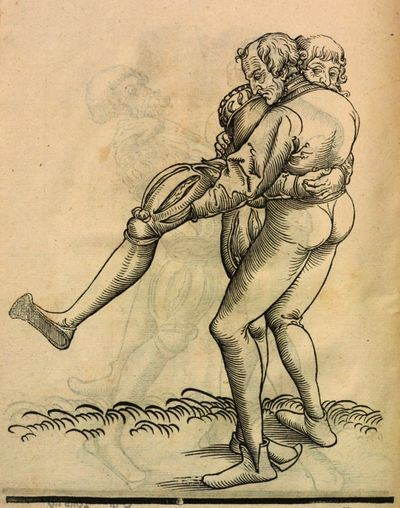
\includegraphics[scale=1.75]{Wasichheb.jpg}
\caption{Göttingen, Universitätsbibliothek, 2° Cod. Ms. philos. 62, fol 25r.}
\end{figure}

\newpage

\begin{center}
    \minisec{Notizen}
    \liniert[1cm]{18}
\end{center}
\newpage

\subsubsection[Armringen I]{Armringen I\footnote{\hspace*{0.5ex}Rom, Biblioteca dell'Accademia Nazionale dei Lincei e Corsiniana, Cod. 1449 (Standortnummer 44 A 8), fol. 33r-33v, Transkription und Übersetzung: Dierk Hagedorn.}}

\begin{longtable}{p{6.25cm}p{6.25cm}}
\textbf{\textcolor{red}{Hier merck nw die arm\textasciitilde  ringen Im swert}}
&
\textbf{\textcolor{red}{Das Armringen am Schwert}}
\\
\\
| Merck wenn er dir ein laufft Im swert | vnd helt sein hentt nider | So verker dein lincke hant | vnd begreiff do mit sein rechte Innwendig zwischen seine\textasciitilde  paiden | henden vnd ruck in do mit auff dein lincke seitten | vnd mit der rechten slach in mit dem swert vber den kopff | Oder | wiltu In nicht slachen | So spring mit dem rechten fuess hinder seinen dencken | vnd var Im mit dem rechtñ arm\textasciitilde  vorñ vor oder hinden vmb den hals | vnd wurff In also vber dein rechts knÿe \textasciitilde 
&
Wenn er dir mit dem Schwert einläuft und dabei die Hände unten hält, verdreh deine linke Hand und greif damit seine rechte auf der Innenseite zwischen seinen beiden Händen. Reiß ihn so auf deine linke Seite und schlag ihm mit der rechten mit dem Schwert auf den Kopf. Wenn du ihn hingegen nicht schlagen willst, dann spring mit dem rechten Fuß hinter seinen linken und fahr ihm mit dem rechten Arm vorne oder hinten um den Hals und wirf ihn somit über dein rechtes Knie.
\end{longtable}

\newpage

\begin{center}
    \minisec{Notizen}
    \liniert[1cm]{18}
\end{center}

\newpage

\subsubsection[Schwertnehmen I]{Schwertnehmen I\footnote{\hspace*{0.5ex}Rom, Biblioteca dell'Accademia Nazionale dei Lincei e Corsiniana, Cod. 1449 (Standortnummer 44 A 8), fol. 33v-34r, Transkription und Übersetzung: Dierk Hagedorn.}}

\begin{longtable}{p{6.25cm}p{6.25cm}}
\textbf{\textcolor{red}{Hie merck ein swert nemen}}
&
\textbf{\textcolor{red}{Ein Schwertnehmen}}
\\
\\
| Merck wenn man dir ein lauf Im swert | So verker dein lincke hant | vnd var do mit vber sein rechten arm\textasciitilde  | vnd begreiff do mit sein swert zwischen seinen paiden hendñ peÿ der hanthab | vnd ruck do mit auff dein lincke seitten | So nÿmpstu Im sein swert
&
Wenn man dir mit dem Schwert einläuft, verdreh deine linke Hand und fahr damit über seinen rechten Arm. Greif sein Schwert zwischen seinen beiden Händen am Griff und reiß es daran auf deine linke Seite. So nimmst du ihm sein Schwert.
\end{longtable}

\newpage

\begin{center}
    \minisec{Notizen}
    \liniert[1cm]{18}
\end{center}
\newpage

\subsection{Die 3 Wunder - Häue, Stiche, Schnitte aus den Huten}\label{Wunder}

\begin{center}
\resizebox{\textwidth}{!}{\textbf{3 Wunder | Blößen nutzen | Die Schwache Bindung | Kurze/Lange Schneide | Timing}}
\end{center}
Diese Lektion soll über das generelle Fechten mit Häuen hinaus gehen. Speziell soll dies anhand der von Liechtenauer beschrieben drei Wunder also Stich, Schnitt und Hau geschehen.
\\
\\
Dafür wird zunächst besonderes Augenmerk auf die Ausführung des Stiches aus verschiedenen Huten und zu verschiedenen Blößen gelegt. Im gleichen Zug soll dem eine möglichst effiziente Versatzung gegenübergesetzt werden.
\\
\\
Anschließend wird über das \textbf{Absetzten} der Stich in ein fechteriches Gesamtkonzept gesetzt, um so Möglichkeiten zur Ausführung aus dem Gefechtsverlauf zu geben.
\\
\\
Darauf folgend werden mit dem \textbf{Ansetzen} und weiterhin dem \textbf{Abschneiden} die Verwendung von Schnitten im Gefechtsverlauf dargestellt. Besonderes Augenmerk soll hier auf das Erkennen der dafür benötigten Blößen und dem Ausführungszeitpunkt gelegt werden.
\\
\\
Schließlich soll zum dritten Wunder, dem Hau, besonders auf Häue mit der kurzen Schneide und deren Vorteile eigegangen werden, um die Versatilität der Fechtenden zu fördern. Deren Durchführung wird zunächst allgemein durch Übung mit verschieden Huten und Häuen trainiert und nochmals exemplarisch durch das Schnappen und den \textbf{Twerhau} als Meisterhau demonstriert.
\\
\\
Diese Lektion vermittelt den Fechtenden das Wissen um die diversen Nutzungsmöglichkeiten des Schwerts neben dem Fechten mit Häuen. Es werden speziell die Konzepte der kurzen und langen Schneide und des Fechten zu den Blößen behandelt.
\\
\\
Stücke und Schwerpunkte:
 
\begin{itemize}
    \item Twerhau
    \item Absetzen Oben/Unten (als Ausgang zum Stich)
    \item Ansetzen/Abschneiden (als Ausgang zum Schnitt)
\end{itemize}

\hspace{0.5cm}

\begin{itemize}
    \item Stiche (Ausführung und Versatzung)
    \item Häue mit kurzer Schneide/Schnappen
    \item Meisterhau mit beiden Schneiden
\end{itemize}

\newpage
\null
\thispagestyle{empty}
\newpage

\subsubsection[Twerhau]{Twerhau\footnote{\hspace*{0.5ex}Rom, Biblioteca dell'Accademia Nazionale dei Lincei e Corsiniana, Cod. 1449 (Standortnummer 44 A 8), fol. 18v-19r, Transkription und Übersetzung: Dierk Hagedorn.}}

\begin{longtable}{p{6.25cm}p{6.25cm}}
\textbf{\textcolor{red}{Hie hebt sich an der text vnd die glos von dem twer haw mit seinen stucken}}
&
\textbf{\textcolor{red}{Der Twerhau mit seinen Stücken}}
\\
\\
\textcolor{red}{Twer benÿmpt was vom tag her chumpt}
&
\textcolor{red}{Der Twerhau wehrt ab, was vom Tag her kommt.}
\\
\\
| Glosa | Merck der twer haw pricht die hu°t vom tag | vnd alle haw die von oben nÿder gehauen werden | vnd die twer treib also | wenn du mit dem | zu° ÿm kumpst | So stee mit dem lincken fuess vor | vnd halt dein swert an deiner rechten achsel | Stet er denn gegen dir | vnd helt sein swert mit auff gerackten armen hoch vber dem haubt | vnd drot dir oben ein zw° hauen | So kum du vor im mit dem haw | vnd spring mit dem rechten fuess wol auff dein rechte seitten gegen ÿm | vnd ÿm sprung wind dein swert mit dem gehültz für dein haubt | das dein dawmen vnden küm | vnd slach ÿm mit der kurtzen schneid gegen seiner lincken seitten zw dem kopff
&
Der Twerhau bricht die Hut vom Tag sowie alle Hiebe, die von oben herab geschlagen werden.
Führ den Twerhau auf diese Weise aus: Wenn du im [Zufechten] zu ihm kommst, steh mit dem linken Fuß vor und halt dein Schwert an deiner rechten Schulter. Wenn er mit dem Schwert mit hoch über dem Kopf aufgereckten Armen vor dir steht und droht, einen Oberhau zu schlagen, dann komm ihm mit dem Hieb zuvor. Spring mit dem rechten Fuß entschieden auf deine rechte Seite, ihm entgegen. Winde im Sprung dein Schwert mit dem Gehilz vor deinen Kopf, so daß der Daumen unten liegt, und schlag ihm mit der kurzen Schneide zu seiner Linken zum Kopf.
\\
\\
\textcolor{red}{Oder}
&

\\
\\
| kumpt er vor mit dem haw von oben nÿder ee wenn dw | So spring mit dem rechten fuess aus dem haw wol auff dein rechte seitten mit der vor geschriben vor satzung | So vechstu seine\textasciitilde  haw in dein gehültz | vnd slach ÿn mit der twer zu° der lincken seitten seines kopffs \textasciitilde 
&
Wenn er hingegen seinen Hieb von oben herab früher als du schlägt, spring mit dem rechten Fuß entschieden auf deine rechte Seite, vom Hieb weg, und versetz dabei auf die eben beschriebene Weise. So fängst du seinen Hieb mit deinem Gehilz. Schlag ihm dann mit dem Twerhau zur linken Seite seines Kopfes.
\end{longtable}

\newpage

\begin{center}
    \minisec{Notizen}
    \liniert[1cm]{18}
\end{center}
\newpage

\subsubsection[Absetzen Oben/Unten]{Absetzen Oben/Unten\footnote{\hspace*{0.5ex}Rom, Biblioteca dell'Accademia Nazionale dei Lincei e Corsiniana, Cod. 1449 (Standortnummer 44 A 8), fol. 30r-30v, Transkription und Übersetzung: Dierk Hagedorn.}}

\begin{longtable}{p{6.25cm}p{6.25cm}}
\textbf{\textcolor{red}{Hier merck das ist der text vnd die glos wie man stich vnd haw absetzen sol}}
&
\textbf{\textcolor{red}{Wie man Stiche und Hiebe absetzen soll}}
\\
\\
\textcolor{red}{lere absetzen häw stich kunstlich letzen wer auf dich sticht dein ort trifft vnd seinen pricht Von paiden seitten Triff allemal wildu schreitten}
&
\textcolor{red}{Lern das Absetzen von Hieb und Stich und geschickt den zu verletzen, der auf dich sticht. Dein Ort trifft und bricht seinen. Triff auf beiden Seiten jederzeit, wenn du einen Schritt machen willst.}
\\
\\
| Glosa | Merck die absetzen die treib also | wenn dw mit dem zw fechten zw° Im kumpst | stelt er sich denn gegen dir als er dich wöll stechen | So setz den lincken fues vor | vnd stee gegen Im in der hu°t des phluegs von deiner rechten seitten | vnd gib dich plos mit der lincken seitten | Sticht er dir denn zw° der selbigen plöss | So wind mit dem swert auff dein lincke seittñ gegen seine\textasciitilde  stich die kurtz schneid an sein swert | vnd setz da mit ab | vnd schreit do mit zu° mit dem rechten füess | vnd stich Im | Inndes zw dem gesicht oder zw° der prust \textasciitilde 
&
Führ das Absetzen folgendermaßen aus: Wenn du im Zufechten zu ihm kommst und er dir gegenübersteht als wolle er stechen, setz den linken Fuß vor und steh vor ihm in der Hut Pflug auf der rechten Seite. Gib dir also eine Blöße auf der Linken. Sticht er dann zu dieser Blöße, winde mit dem Schwert gegen seinen Stich auf deine linke Seite, und zwar mit der kurzen Schneide an sein Schwert. Setz auf diese Weise ab und mach gleichzeitig einen Schritt mit dem rechten Fuß. Stich ihm »indes« zum Gesicht oder zur Brust.
\\
\\
\textbf{\textcolor{red}{Ein anders stuck}}
&
\textbf{\textcolor{red}{Ein weiteres Stück}}
\\
\\
| Merck | wenn dw stest von dein° rechten seitten in dem phlueg | hawt er dir denn ein zu° deiner lincken seitten oben zw° dem kopff | So var – (getilgter und überschriebener Buchstabe) auff mit dem swert | vnd wind da mit auff dein lincke seittñ gegen seinem haw das gehultz für dein haubt | vnd schreit do mit zw° mit dem rechten füess | vnd stich ÿm zw° dem gesicht oder der prust die stuck treib aus dem phlueg zw° paiden seitten \textasciitilde 
&
Wenn du im rechten Pflug stehst und er dann oben links zu deinem Kopf schlägt, fahr mit dem Schwert auf, und winde gleichzeitig das Gehilz auf deine linke Seite gegen seinen Hieb und vor deinen Kopf. Mach dabei einen Schritt mit dem rechten Fuß und stich ihm zum Gesicht oder zur Brust. Dieses Stück kannst du aus dem Pflug auf beiden Seiten anwenden.
\end{longtable}

\newpage

\begin{center}
    \minisec{Notizen}
    \liniert[1cm]{18}
\end{center}

\newpage

\subsubsection[Ansetzen/Abschneiden]{Ansetzen/Abschneiden\footnote{\hspace*{0.5ex}Rom, Biblioteca dell'Accademia Nazionale dei Lincei e Corsiniana, Cod. 1449 (Standortnummer 44 A 8), fol. 34r-34v, Transkription und Übersetzung: Dierk Hagedorn.}}

\begin{longtable}{p{6.25cm}p{6.25cm}}
\textbf{\textcolor{red}{Hie merck den text vnd die glos von abschneÿden}}
&
\textbf{\textcolor{red}{Das Abschneiden}}
\\
\\
\textcolor{red}{Schneid ab die herten von vnden In paiden gefertten}
&
\textcolor{red}{Schneid die kräftigen Hiebe von unten mit beiden Angriffen ab.}
\\
\\
| Glosa merck | das ist was dw solt treibñ | wenn man dir starck oben auff dein swert pintt oder dar auff velt | vnd das vernÿm also v Wenn du zu° vichtest aus den vnder häwen | oder aus den streichen oder ligst gegen Im In der hu°t alber | Velt er dir denn mit dem swert | auff das dein ee wenn du do mit auff ku\textasciitilde pst | So pleib vnden an dem swert | vnd heb mit der kurtzen schneid vast vber sich | Druckt er denn dein swert vast nyder | So streich vnden mit deinem swert mit an seiner swertz klingen hinder sich ab von seinem swert | vnd haw In zw° der anderñ seitten an seinem swert pald wider oben ein zw° dem maul \textasciitilde 
&
Dies ist zu tun, wenn man dir stark oben auf dein Schwert bindet oder darauf fällt. Man hat es sich so vorzustellen: Wenn du im Zufechten mit einem Unterhau oder dem Streichen angreifst oder ihm in der Hut Alber entgegenstehst und er dir mit dem Schwert auf das deine fällt, bevor du es erheben konntest, so bleib unten am Schwert und heb es mit der kurzen Schneide schnell nach oben. Drückt er dann dein Schwert kräftig nach unten, streich unten mit deinem Schwert an seiner Klinge nach hinten von seinem Schwert weg, und schlag ihm auf der anderen Seite an seinem Schwert sofort erneut oben zum Mund.
\end{longtable}

\newpage

\begin{center}
    \minisec{Notizen}
    \liniert[1cm]{18}
\end{center}

\newpage

\subsection{Bindung II}  \label{Bindung2}

\begin{center}
\resizebox{\textwidth}{!}{\textbf{Stärke | Ort des Anbindung | Prinzip der Kurzen Wege | Fechten zum:zur Gegner:in}}
\end{center}
Gegenüber Bindung I setzt diese Lektion mit Techniken an, welche ebenfalls ein Fühlen bzw. ein Verständnis der Bindung voraussetzen. Nachdem in der Wiederholung bereits die Bedeutung der Überbindung in der Schwäche des:der Gegner:in herausgestellt wurde, wechselt nun der Fokus auf den Fall, dass wir uns entweder in der Stärke befinden oder eine Überbindung nicht möglich ist. Die Erkenntnis besteht darin, die Seite der Anbindung zu wechseln (und dazu die Bindung kurzeitig lösen), um die Kraftrichtung der gegnerischen Klinge nach Außen laufen zu lassen und gleichzeitig selbst eine Bedrohung aufzubauen. Dies schult zugleich, den Druck zum:zur Gegner:in und nicht zur Waffe zu richten (auch hierzu gibt es Ausnahmen, z.B.: den Zornhau).
\\
\\
\textbf{Oben Abnehmen} stellt hierbei den klassischen Fall dar, dass der:die Gegner:in fehlerhafterweise einen Oberhau zum Schwert schlägt und ggf durch Krafteinsatz eine Überbindung erzwingen will. Das Oben Abnehmen stellt dann ein schnelles und einfach zu erlenendes Grundprinzip dar, wann eine kurze Lösung von der Bindung ausreichend ist, um rechtzeitig und gedeckt seine:n Gegner:in von der anderen Seite zu treffen, bzw. eine vorteilhaftere Bindung herzustellen.
\\
\\
Das \textbf{Durchwechseln} wird anschließend als passendes Gegenstück von unten dargestellt, wobei dieses um den Teil des bindungslosen Eintretens ergänzt wird. Im Speziellen bedeutet dies ein Zufechten im Langort/Pflug mit Durchwechseln vor der ersten Anbindung.
\\
\\
Stücke und Schwerpunkte:

\begin{itemize}
    \item Durchwechseln
    \item Zucken
    \item Zornhau-Ort
    \item Zornhau-Ort mit Oben Abnehmen
\end{itemize}

\newpage
\null
\thispagestyle{empty}
\newpage

\subsubsection[Durchwechseln]{Durchwechseln\footnote{\hspace*{0.5ex}Rom, Biblioteca dell'Accademia Nazionale dei Lincei e Corsiniana, Cod. 1449 (Standortnummer 44 A 8), fol. 30v-31r, Transkription und Übersetzung: Dierk Hagedorn.}}

\begin{longtable}{p{6.25cm}p{6.25cm}}
\textbf{\textcolor{red}{Das ist der text mit der glos wie man sol durchwechselñ}}
&
\textbf{\textcolor{red}{Wie man durchwechseln soll}}
\\
\\
\textcolor{red}{Durchwechsel lere von paiden seitten stich mit sere wer auf dich pindet Durchwechsel In schir vindet}
&
\textcolor{red}{Lern das Durchwechseln auf beiden Seiten. Stich und verletz den, der dich bindet. Durchwechseln findet ihn sofort.}
\\
\\
| Glosa | Merck der durchwechsel ist vil | vnd manigerlaÿ | Die soltu treiben gegen den vechterñ | die do gerñ vorsetzen | vnd die do hawen | zw dem swert | vnd nicht zw° den plössen des leibs | Die soltu gar wol lernen treiben mit fürsichtigkait | das mann dir icht an setz | oder sünst ein kum dieweil du durchwechselst
&
Es gibt vielerlei unterschiedliche Möglichkeiten durchzuwechseln. Das Durchwechseln soll gegen solche Fechter angewandt werden, die gerne versetzen und zum Schwert anstatt zu den Blößen des Körpers schlagen. Du sollst das Durchwechseln sicher und umsichtig auszuführen lernen, damit man dir nicht ansetzt oder dich anderweitig trifft, während du durchwechselst.
\\
\\
\textbf{\textcolor{red}{Die durchwechsel treib Also}}
&
\textbf{\textcolor{red}{Führ das Durchwechseln folgendermaßen aus}}
\\
\\
| Wenn dw mit dem zw° uechten zw Im kumpst | So haw im oben starck ein | hawt er denn wider gegen dir zw° dem swert vnd nicht zu° dem leib | So lass den ort mit dem haw vnden durch sein swert wischen | ee | wenn er dir an das swert pindt | vnd stich Im zw° anderñ seittñ zw der prust | wirt er denn des stichs gewar | vnd vert mit dem swert dem stich pald nach mit vor satzu\textasciitilde g | So wechsel aber durch | vnd das thue albeg wenn er dir mit vor setzen nach dem swert vert
&
Wenn du im Zufechten zu ihm kommst, schlag kräftig oben zu ihm. Schlägt er dann gegen dein Schwert und nicht zum Körper, laß den Ort in der Hiebbewegung unter seinem Schwert hindurchgleiten, bevor er an dein Schwert bindet. Stich ihm dann auf der anderen Seite zur Brust. Wenn er den Stich bemerkt und ihm mit einer Versatzung nacheilt, wechsel erneut durch. Mach dies jedesmal, wenn er dir zum Schwert hin versetzt.
\end{longtable}

\newpage

\begin{center}
    \minisec{Notizen}
    \liniert[1cm]{18}
\end{center}

\newpage

\begin{longtable}{p{6.25cm}p{6.25cm}}
Oder • 
&
Oder,
\\
| Wenn dw mit dem zü fechten zw Im kumpst | So setz den lincken fues vor | vnd halt Im den langen ort gegen dem gesicht | hawt er dir deñ von oben nider oder von unden auff zw dem swert | vnd wil dir das wegck slahen oder starck dar an pinden | So lass den ort vndersich sencken | vnd stich Im zw° der anderñ seitten das treib gegen | allen häwen | do mit man dir zu° dem swert hawt
&
wenn du im Zufechten zu ihm kommst, setz den linken Fuß vor und halt ihm den Langort zum Gesicht. Schlägt er dann von oben herab oder von unten hoch zu deinem Schwert, um es dir wegzuschlagen oder stark anzubinden, so laß den Ort nach unten sinken und stich ihn auf der anderen Seite. Wende dies gegen alle Hiebe an, mit denen man dir zum Schwert schlägt.
\end{longtable}

\newpage

\begin{center}
    \minisec{Notizen}
    \liniert[1cm]{18}
\end{center}

\newpage

\subsubsection[Zucken]{Zucken\footnote{\hspace*{0.5ex}Rom, Biblioteca dell'Accademia Nazionale dei Lincei e Corsiniana, Cod. 1449 (Standortnummer 44 A 8), fol. 31v-32r, Transkription und Übersetzung: Dierk Hagedorn.}}

\begin{longtable}{p{6.25cm}p{6.25cm}}
\textbf{\textcolor{red}{Hie merck den text vnd die glos von den zucken am swert}}
&
\textbf{\textcolor{red}{Das Zucken am Schwert}}
\\
\\
\textcolor{red}{Trit nahent in pünden das zucken gibt gu°te fünde Zuck trift er zuck mer Arbait erfinde Das thuet ÿm we Zuck allen treffen den maisterñ wiltu sy effen}
&
\textcolor{red}{Tritt beim Anbinden näher. Das Zucken gibt gute Treffermöglichkeiten. Zuck. Trifft er, zuck erneut. Finde Angriffsmöglichkeiten. Dies schmerzt ihn. Zuck bei jedem Aufeinandertreffen, wenn du die Meister narren möchtest.}
\\
\\
| Glosa | merck das zucken gehört zu° treibñ gegen den maisterñ die do starck an das swert pinden | vnd am pant des swertz beleiben still sten | vnd wöllen warten ob man sich für In ab wolt hawen oder vom swert ab tzÿehen | Das sÿ denn möchten nachgeraisen zu° der plöss | Wiltu die | selbigen maister ëffen oder tewschen | So treib die zucken gegen Im also | haw ÿm von der rechten seitten oben starck ein zw dem kopff | vert er denn mit dem swert starck für mit dem haw | vnd wil vor setzen oder haut dir zw° dem swert | So zuck dein swert an dich | ee | wenn er dir an pint | vnd stich Im zw° der anderñ seittñ | vnd das dw gegen allen treffen | vnd an pinden des swertz \textasciitilde 
&
Das Zucken soll gegen solche Meister angewandt werden, die stark an das Schwert binden und im Band des Schwertes stillstehen bleiben und darauf warten, daß man sich vor ihnen abschlägt oder vom Schwert abzieht. Denn so können sie zu einer Blöße nachreisen. Wenn du diese Meister narren oder täuschen willst, wende das Zucken folgendermaßen an: Schlag von der rechten Seite kräftig oben zum Kopf. Kommt er dann mit dem Schwert mit einem Hieb weit nach vorne, um dir zu versetzen, oder wenn er dir zum Schwert schlägt, so zuck dein Schwert zu dir, bevor er dir anbindet. Stich ihm auf die andere Seite. Tu dies gegen jegliches Aufeinandertreffen oder Anbinden der Schwerter.
\end{longtable}

\newpage

\begin{center}
    \minisec{Notizen}
    \liniert[1cm]{18}
\end{center}
\newpage

\subsubsection[Zornhau]{Zornhau\footnote{\hspace*{0.5ex}Rom, Biblioteca dell'Accademia Nazionale dei Lincei e Corsiniana, Cod. 1449 (Standortnummer 44 A 8), fol. 13r-13v, Transkription und Übersetzung: Dierk Hagedorn.}}

\begin{longtable}{p{6.25cm}p{6.25cm}}
\textbf{\textcolor{red}{Merck hÿe hebt sich an der text vnd die glos}}
&
\textbf{\textcolor{red}{Der Zornhau mit seinen Stücken}}
\\
\\
| Des ersten von dem zorñhäw mit seinen stucken
&

\\
\\
\textcolor{red}{Wer dir oberhawt zorñhaw ort dem drawt}
&
\textcolor{red}{Wer einen Oberhau zu dir schlägt, dem droht der Zornhau-Ort.}
\\
\\
| Glosa | Merck der zorñhaw pricht mit dem ort alle oberhaw | vnd ist doch anders nicht | wenn ein slächter paurñ slagk | vnd den treib also | Wenn dw mit dem zu° vechten zu ym kumst | haut er dir denn von seiner rechtñ seitten oben ein zu° dem kopff | So haw auch von dein° rechten seitten von oben an alle vor satzung | Mit im zornigklich ein auf sein swert | Ist er denn waich öm swert | so seüß im den ort gericht für sich lanck ein | vnd stich im zu° dem | gesicht oder der prüst | So setz im an
&
Der Zornhau bricht mit dem Ort alle Oberhaue und ist doch nichts anderes als ein schlichter Bauernschlag. Führ ihn aus wie folgt: Wenn du im Zufechten zu ihm kommst und er dir von seiner rechten Seite oben zum Kopf schlägt, schlag auch du von deiner rechten Seite von oben ohne jegliche Versatzung gleichzeitig heftig auf sein Schwert. Ist er dann weich am Schwert, stoß mit dem Ort geradeaus lang auf ihn ein und stich ihm zum Gesicht oder zur Brust. Setz ihm so an.
\end{longtable}

\newpage

\begin{center}
    \minisec{Notizen}
    \liniert[1cm]{18}
\end{center}

\newpage

\begin{longtable}{p{6.25cm}p{6.25cm}}
\textbf{\textcolor{red}{Das ist der text vnd die glos aber eins stuck des zorñ haus}}
&
\textbf{\textcolor{red}{Ein weiteres Stück vom Zornhau}}
\\
\\
\textcolor{red}{Wirt er es gewar So nÿm oben ab ane far}
&
\textcolor{red}{Bemerkt er es, nimm oben ohne Gefahr ab.}
\\
\\
| Glosa | Merck das ist | wenn du nn im mit dem zorñhaw ein haust | So seuß im den ort lanck ein zu dem gesicht oder prüst als vor geschriben stet | wirt er denn orts gewar | vnd vor setzt starck | vnd druckt dir dein swert auf die seittñ | So reiß mit deinem swert an seiner swertz clingen vber sich auf oben ab von seinem swert | vnd haw ÿm zw der anderñ seitten aber an seiner swertz klingen wider ein zu° dem kopff das haist oben ab genomen | Also prich das wenn er oben ab nÿmpt so pind an seinem swert starck oben ein ze seinem kopff mit der langen schneid \textasciitilde 
&
Wenn du mit dem Zornhau zu ihm schlägst, stoß ihm den Ort lang zum Gesicht oder zur Brust, wie oben beschrieben. Bemerkt er dann den Ort und versetzt kräftig, indem er dein Schwert zur Seite drückt, reiß dein Schwert an seiner Klinge hoch und oben weg von seinem Schwert. Schlag ihm auf der anderen Seite wiederum an seiner Schwertklinge zum Kopf. Dies nennt man oben abnehmen. Brich dies folgendermaßen: Wenn er oben abnimmt, binde mit der langen Schneide an seinem Schwert kräftig in Richtung auf seinen Kopf.
\end{longtable}

\newpage

\begin{center}
    \minisec{Notizen}
    \liniert[1cm]{18}
\end{center}

\newpage

\subsection{Ringen II}
\subsubsection[Die Huffe desz Elnbogens]{Die Huffe desz Elnbogens\footnote{\hspace*{0.5ex}Göttingen, Niedersächsische Staats- und Universitätsbibliothek Göttingen, 2° Cod. MS. Philos.62, fol. 29v-30r, Transkription von Thore Wilkins}}

\textbf{[29v] Die Huffe desz Elnbogens}
\\
\\
\textbf{Wen} mich einer vorn ins wams faßet so wische ich mit meinem elnbogen hart an seine faust, vnd gebe mich nieder in die wage, so reis ich mit meinem elnbogen seine faust heraus, vnd gebe mich auf, folge mit meiner rechten hand nach, trete mit meinem rechten schenckel naus, vnd nehme die rechte huffe, die gehet gewaltiglich.
\\
\\
\textbf{[30r] Zur .26. figura explicatio von der hufte oder achsell des Elnbogens solte billig die achsel heißen.}
\\
\\
In dieser \textbf{figura} gedenckt der \textbf{Autor} des wammes seines leibes, da er dan seinem kegenteil den erßten griff erlaubet, zeiget auch darnach weiter an das er sich dem gewichten nach nider sencke, vnd mit seinen ellebogen, das ist mit dem andern deil des arms seines kegentheils erste teil des arms, nemlich die hand oder das erste gelencke hinter der hand angreifft oder ansetzet vnd sich loßmachet, erwischet ihn darnach wiederumb bei dem dritten gelenck des armes vnd hebet den mit seinem ganzen leibe in die hohe, vnd mit der lincken hand ergreifft er seines wiedparts lincken arm, zeugt ihn mit gewalt zu sich vnd wirfft ihn also nach dem gewichte vber die halbe huffe zur erd’ also kan man leichtlich in dieser \textbf{figura} mercken, wie viel im ringen daran gelegen ist, das man die \textbf{juncturas extremitatu corporis burnani} recht greifft vnd anfaßet, vnd nach dem gewicht vnd nach der \textbf{declination} des leibes mit dem bewegen \textbf{procediren} mus, wie beÿ den vorigen \textbf{figuren} zum offtern mal gedacht ist worden.

\begin{figure}[h]
\centering
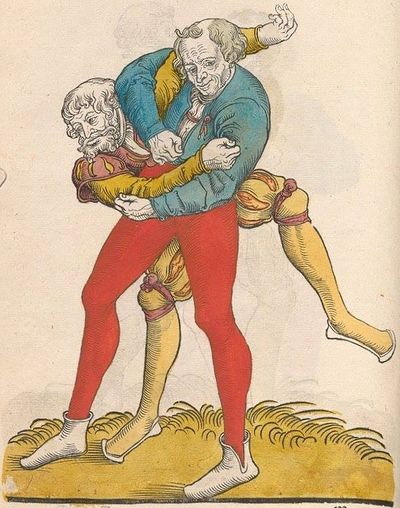
\includegraphics[scale=1.35]{Die_Huffe_desz_Elnbogens.jpg}
\caption{26.figura}\label{Die_Huffe_desz_Elnbogens}
\end{figure}

\newpage
\begin{center}
    \minisec{Notizen}
    \liniert[1cm]{18}
\end{center}
\newpage

\subsubsection[Ein weiteres Armringen (Armringen II)]{Ein weiteres Armringen (Armringen II)\footnote{\hspace*{0.5ex}Rom, Biblioteca dell'Accademia Nazionale dei Lincei e Corsiniana, Cod. 1449 (Standortnummer 44 A 8), fol. 33v, Transkription und Übersetzung: Dierk Hagedorn.}}

\begin{longtable}{p{6.25cm}p{6.25cm}}
\textbf{\textcolor{red}{Aber ein arm\textasciitilde  ringen}}
&
\textbf{\textcolor{red}{Ein weiteres Armringen}}
\\
\\
| Merck | wenn er dir ein laufft Im swert || vñ ist nÿder mit den henden | So lass dein lincke hant varñ vom swert | vnd mit der rechtñ var Im mit dem knopff aussen vber sein rechte hant | vnd druck do mit nÿder | vnd begreiff ÿm mit der lincken hant peÿ seine\textasciitilde  rechten elpogen | vnd spring mit dem denckñ fuess fur sein rechten | vnd stos in also dar vber \textasciitilde 
&
Wenn er dir mit dem Schwert einläuft und dabei die Hände unten hält, laß dein Schwert mit deiner linken Hand los und fahr ihm mit der rechten mit dem Knauf außen über seine rechte Hand. Drück dabei nach unten und greif mit der linken Hand seinen rechten Ellenbogen. Spring mit dem linken Fuß vor seinen rechten und stoß ihn darüber.
\\
\\
\textbf{\textcolor{red}{Aber ein arm\textasciitilde  ringen}}
&
\textbf{\textcolor{red}{Ein weiteres Armringen}}
\\
\\
| Merck | wenn er dir ein laufft im swert | So lass dein swert vallen | vnd ver ker dein rechte hant | vnd begreiff do mit sein rechte auswendige | vnd mit der lincken vaß In peÿ dem rechtñ elpogen | vnd spring mit dem lincken fuess fur sein rechten | vnd stos mit der rechten hant seinen rechtñ arm\textasciitilde  über deinen lincken | vnd heb In do mit vbersich | Also magstu Im den arm\textasciitilde  prechen | oder für dich vber das linck pain werffen ob dw wild
&
Wenn er dir mit dem Schwert einläuft, laß dein Schwert fallen und verdreh deine rechte Hand. Greif damit seine rechte von außen. Faß ihn mit der linken am rechten Ellenbogen und spring mit dem linken Fuß vor seinen rechten. Stoß mit der rechten Hand seinen rechten Arm über deinen linken und heb ihn dabei nach oben. Auf diese Weise kannst du ihm wahlweise den Arm brechen oder ihn vor dich über das linke Bein werfen.
\end{longtable}

\newpage

\begin{center}
    \minisec{Notizen}
    \liniert[1cm]{18}
\end{center}
\newpage

\subsubsection[Ein weiteres Schwertnehmen (Schwertnehmen II)]{Ein weiteres Schwertnehmen (Schwertnehmen II)\footnote{\hspace*{0.5ex}Rom, Biblioteca dell'Accademia Nazionale dei Lincei e Corsiniana, Cod. 1449 (Standortnummer 44 A 8), fol. 34r, Transkription und Übersetzung: Dierk Hagedorn.}}

\begin{longtable}{p{6.25cm}p{6.25cm}}
\textbf{\textcolor{red}{Aber ein swert nemen}}
&
\textbf{\textcolor{red}{Ein weiteres Schwertnehmen}}
\\
\\
| Merck | wenn er dir vorsetzt | oder sünst an dein swert pint | So begreiff mit der lincken hant paide swert mitten in den klingen | vnd halt sÿ paide vest zw° sãmen | vnd var mit der rechten hant vnden durch mit dem knopf vorñ vber sein pede hendt | vnd ruck do mit vbersich auff dein rechte seitten so peleiben dir paide swert \textasciitilde 
&
Wenn er dir versetzt oder sonstwie an dein Schwert bindet, greif mit der linken Hand beide Schwerter in der Mitte der Klingen und halt sie beide fest zusammen. Fahr mit der rechten Hand unten durch und mit dem Knauf vorne über seine beiden Hände. Reiß sie dabei nach oben auf deine rechte Seite, so bleiben dir beide Schwerter.
\end{longtable}

\newpage

\begin{center}
    \minisec{Notizen}
    \liniert[1cm]{18}
\end{center}

\newpage

\section{Anhang}

\subsection{Nützliche Links}\label{Nützliche Links}

\begin{itemize}
    \item \textbf{Wiktenauer}, Onlinesammlung von Fechtbüchern inklusive Transkriptionen und Übersetzungen
    \\
    \\
    Link: wiktenauer.com
    \item \textbf{DDHF}, Webseite des deutschen Dachverbandes für historisches Fechten, enthält Turnierregelwerke, Zugang zur DDHF-Bildungsplattform und dem DDHF-Forschungsforum
    \\
    \\
    Link: ddhf.de
    \item \textbf{DDHF Forschungsforum}
    \\
    \\
    Link: https://ddhf.de/ddhf-forschungsforum
    \item \textbf{Transkription und Übersetzung des 44A8} von Dierk Hagedorn.
    \\
    \\
    Link: https: www.hammaborg.de/de/transkriptionen/peter\_von\_danzig/
    \item \textbf{KdiH}, der Katalog der deutschsprachigen illustrierten Handschriften
    \\
    \\
    Link: https://kdih.badw.de/datenbank/stoffgruppe/38
    \item \textbf{Datenbank mit Kampfbuchsammlung bis 1600} von Eric Burkart
    \\
    \\
    Link: https://fightbooks.uni-trier.de
\end{itemize}

\newpage

\subsection{Quellen}

\subsubsection*{Glossen, Transkriptionen \& Übersetzungen}

\begin{itemize}
    \item \textbf{Glossen zum langen Schwert} nach dem "Cod. 44 A 8"\ in der "Biblioteca dell’Accademia Nazionale dei Lincei e Corsiniana", Rom
    \\ Anonymer Autor
    \item \textbf{Transkription und Übersetzung zum langen Schwert} nach Dierk Hagedorn, siehe \ref{Nützliche Links}
    \item \textbf{Stück zum Aufstreichen} nach ''E.1939.65.357'', ''Ergrundung Ritterlicher Kunst der Fechterey'' (1516)
    \\ von Andre Paurenfeyndt
    \item \textbf{Glossen zum Ringen} nach Göttingen, Staats- und Universitätsbibliothek, 2° Cod. Ms. philos. 62
    \\ von Fabian von Auerswald
    \item \textbf{Transkriptionen zum Ringen} nach Thore Wilkins
\end{itemize}

\newpage

\subsubsection*{Bildquellen}

Schwertspiel e.V., Verein für traditionelle Kampfkunst in Dresden:
\begin{longtable}{p{6.25cm}p{6.25cm}}
\begin{itemize}
    \item Abbildung 1: Die Nomenklatur des Schwertes
    \item Abbildung 2: Hammergriff
    \item Abbildung 3: Daumengriff
    \item Abbildung 4: links
    \item Abbildung 5: frontal
    \item Abbildung 6: rechts
    \item Abbildung 7: links
    \item Abbildung 8: frontal
    \item Abbildung 9: rechts
    \item Abbildung 10: Ochs rechts
    \item Abbildung 11: Ochs rechts
    \item Abbildung 12: Ochs rechts
    \item Abbildung 13: Ochs links
\end{itemize}

&

\begin{itemize}
    \item Abbildung 14: Ochs links
    \item Abbildung 15: Ochs links
    \item Abbildung 16: links
    \item Abbildung 17: frontal
    \item Abbildung 18: rechts
    \item Abbildung 22: Die Zufechtmensur
    \item Abbildung 23: Eintritt in die Kriegsmensur
    \item Abbildung 24: Austritt aus der Kriegsmensur
    \item Abbildung 25: Das Armringen
    \item Abbildung 26: Das Leibringen
    \item Oberhau
    \item Unterhau
    \item Unterschnitt
\end{itemize}
\end{longtable}
\hspace{3cm}

Wiktenauer, siehe \ref{Nützliche Links}:

\begin{longtable}{p{6.25cm}p{6.25cm}}
\begin{itemize}
    \item Abbildung 19: Vom Tag und Alber
    \item Abbildung 20: Ochs und Pflug
    \item Abbildung 21: Darstellung der Blößen
\end{itemize}

&

\begin{itemize}
    \item Abbildung 27: 22.figura
    \item Abbildung 28: 26.figura
\end{itemize}
\end{longtable}

\end{document}
